\documentclass[12pt,twoside]{article}

\usepackage{float}
\usepackage[english]{babel}
\usepackage[utf8]{inputenc}
\usepackage{amsmath}
\usepackage{graphicx}
\usepackage{epsfig}
\usepackage[table]{xcolor}
\usepackage{multirow}
\usepackage[colorinlistoftodos]{todonotes}
\usepackage[hidelinks]{hyperref}
\usepackage[a4paper,hmargin=2cm,vmargin=0.8cm,includeheadfoot]{geometry}
\usepackage[font=footnotesize]{caption}
\usepackage{natbib}
%\bibliographystyle{ieeetr}
\bibliographystyle{abbrvnat}
\setcitestyle{authoryear,open={(},close={)}} %Citation-related commands

\usepackage{authblk}

% line numbers
\usepackage[right]{lineno} % JG_ADD
\linenumbers
\modulolinenumbers[1]

\raggedbottom 
\linespread{1.25} 

\title{A comprehensive investigation of intracortical and corticothalamic models of alpha rhythms}

\author[1,2]{Sorenza P. Bastiaens}
\author[2,3]{Davide Momi}
\author[1,2]{John D. Griffiths}
\affil[1]{Institute of Medical Sciences, University of Toronto}
\affil[2]{Krembil Centre for Neuroinformatics, Centre for Addiction and Mental Health, Toronto}
\affil[3]{Department of Psychiatry and Behavioral Sciences, Stanford University Medical Center, Stanford, California}

\date{March 2024}

\begin{document}
\maketitle

%TC:ignore
\begin{abstract}
Alpha rhythms are a robust phenomenon prominently observed in posterior resting state electroencephalogram (EEG) that has been shown to play a key role in a number of cognitive processes. However, the underlying mechanisms behind their generation is poorly understood. Here, we showcase the most concrete, mathematically-expressed theoretical foundations for understanding the neural mechanisms underlying the alpha rhythmogenesis. The neural population models of interest are Jansen-Rit (JR), Moran-David-Friston (MDF), Robinson-Rennie-Wright (RRW), and Liley-Wright (LW). Common elements between all models are identified, such as the description of each neural population in the form of a second-order differential equation with a potential-to-rate operator represented as a sigmoid and a rate-to-potential operator usually expressed as an impulse response. Even though these models have major differences, they can be meaningfully compared by associating parameters of analogous biological significance, which we summarize with a unified parameter table. With these correspondences, rate constants and connectivity parameter space is explored to identify common patterns between similar behaviors, such as the role of excitatory-inhibitory interactions in the generation of oscillations. Through stability analysis, two different alpha generation mechanisms were identified: one noise-driven and one self-sustaining oscillation in the form of a limit cycle emerging due to a Andronov-Hopf bifurcation. This work contributes to improving our mechanistic and theoretical understanding on candidate theories of alpha rhythmogenesis.

\end{abstract}
%TC:endignore
\newpage
\tableofcontents


%- Technically oriented summary; 
%- Alpha rhythms are important
%- We review the most prominent mathematical models of alpha rhythm activity in terms of their wiring topology, dynamics, linearized forms, parameterization, and biological interpretation. 
%- The models are x,y,z 
%- They have common elements (sigmoid, impulse response). 
%- They differ in terms of blah 
%- We make that unified parameter table across models
%- Correspondences across models are found / studied in terms of E/I loops etc and their effects on linearized system stability and dynamical regimes
%- This is useful because x 


\newpage
%TC:ignore
\section{Background}
\subsection{Overview and aims}
%TC:endignore
The classical alpha rhythm is an 8-12Hz oscillatory activity pattern that is highly prominent in electroencephalogram (EEG), electrocorticogram (EcoG), and local field potential (LFP) recordings from humans and other species, particularly during states of quiet wakefulness (Fig. 1, A1 and A2). Almost 100 years after its discovery \citep{berger1929elektroenkephalogramm}, alpha frequency activity remains one of the most robustly observed and broadly significant phenomena in all of neuroscience, yet also one of the most enigmatic \citep{bollimunta2011neuronal}. Alpha plays a fundamental role in a wide range of cognitive processes, and abnormal alpha rhythms are frequently identified in psychiatric and neurological conditions as summarized in Fig. 1, A3 \citep{bucci2004executive, clancy2017restless,deiber2020linking,jensen2010shaping}. However, despite the profound importance of alpha rhythms - both in terms of their undeniable prominence in empirical EEG data, and their implication across a broad range of phenomena across clinical and cognitive neuroscience, their mechanistic physiological basis and functional significance remains unclear. Several theories of alpha rhythmogenesis have been proposed over the years, often emphasizing different physiological substrates such as recurrent activity and excitatory-inhibitory interactions in cortical column microcircuits, or delayed inhibitory feedback within cortico-thalamocortical loops (Fig. 1, B2). There have however been relatively few attempts to evaluate and compare in detail these alternative theories in conjunction, and thereby arrive at a useful synthesis of the most compelling accounts. Developing such a synthesis is a principal aim of the present study. 

A central criterion around which we base this investigation is the requirement that the models of interest should be expressed in concrete mathematical language, as well as being implemented in numerical simulations and/or quantitative analytic computations. Specifically, we consider a particular type of neurophysiological model - neural population models (NPMs) (Fig. 1, C1) -  that have been used extensively over the past half century as a tool to better understand alpha activity  \citep{da1977cortical,grimbert2006bifurcation,jansen1995electroencephalogram,liley2001spatially,bhattacharya2011thalamo,david2003neural,hartoyo2019parameter,robinson2003neurophysical}. 
%By analyzing and comparing the implicated circuits in terms of their dynamics, topologies, and parameters, we are able to extract further mechanistic insights into these principal models and theories of alpha rhythmogenesis. 
We focus on four extensively studied NPMs that are commonly used to describe EEG alpha activity in the neuroimaging, neurophysiology, and computational neuroscience literature. We refer to these as the Jansen-Rit (JR; \citealt{jansen1995electroencephalogram}), Moran-David-Friston (MDF; \citealt{david2003neural, moran2007neural}), Liley-Wright (LW;  \citealt{liley1999continuum, liley2001spatially}), and Robinson-Rennie-Wright (RRW; \citealt{robinson2002dynamics, robinson2003neurophysical}) models. These shorthand terms reference certain key individuals who contributed to the conception and/or development of several prominent strands in the research literature. We do note however that they are imperfect ones - both because all of the models studied here build directly on the earlier work of other important theoreticians (e.g. Freeman, Zetterberg, Lopes Da Silva, Cowan, Nunez), and also in some cases each other (e.g. MDF is an indirect extension of JR). 
We begin over the next few sections with a description of general elements present in the JR, MDF, LW, and RRW models, and a summary of their individual  characteristics. Direct comparisons between each of them are then made, first in the context of the alpha regime, and then extending into other oscillatory regimes at non-alpha frequencies.
A central objective in this work is to identify common patterns between the models, using numerical simulations and linear analysis across a broad parameter space to identify the effects of rate constants, inter-population connectivity structure, and other factors on oscillatory dynamics. These similarities and differences across models constitute the points of agreement and divergence across current theories of alpha rhythmogenesis, and it is the mapping of this theoretical landscape that is our main aim in the present paper. The origin, biological significance, and validity of their parameters, as well as the functional forms of their equations, are also considered when discussing the respective limitations and advantages of each candidate model. 
 \
%(maybe finish on alpha theories as well? Or like how can use models to further explore alpha origin? Outline has changed a bit since need to make sure it corresponds) \\

\newpage 
%TC:ignore
\begin{figure}[H]
    \centering
    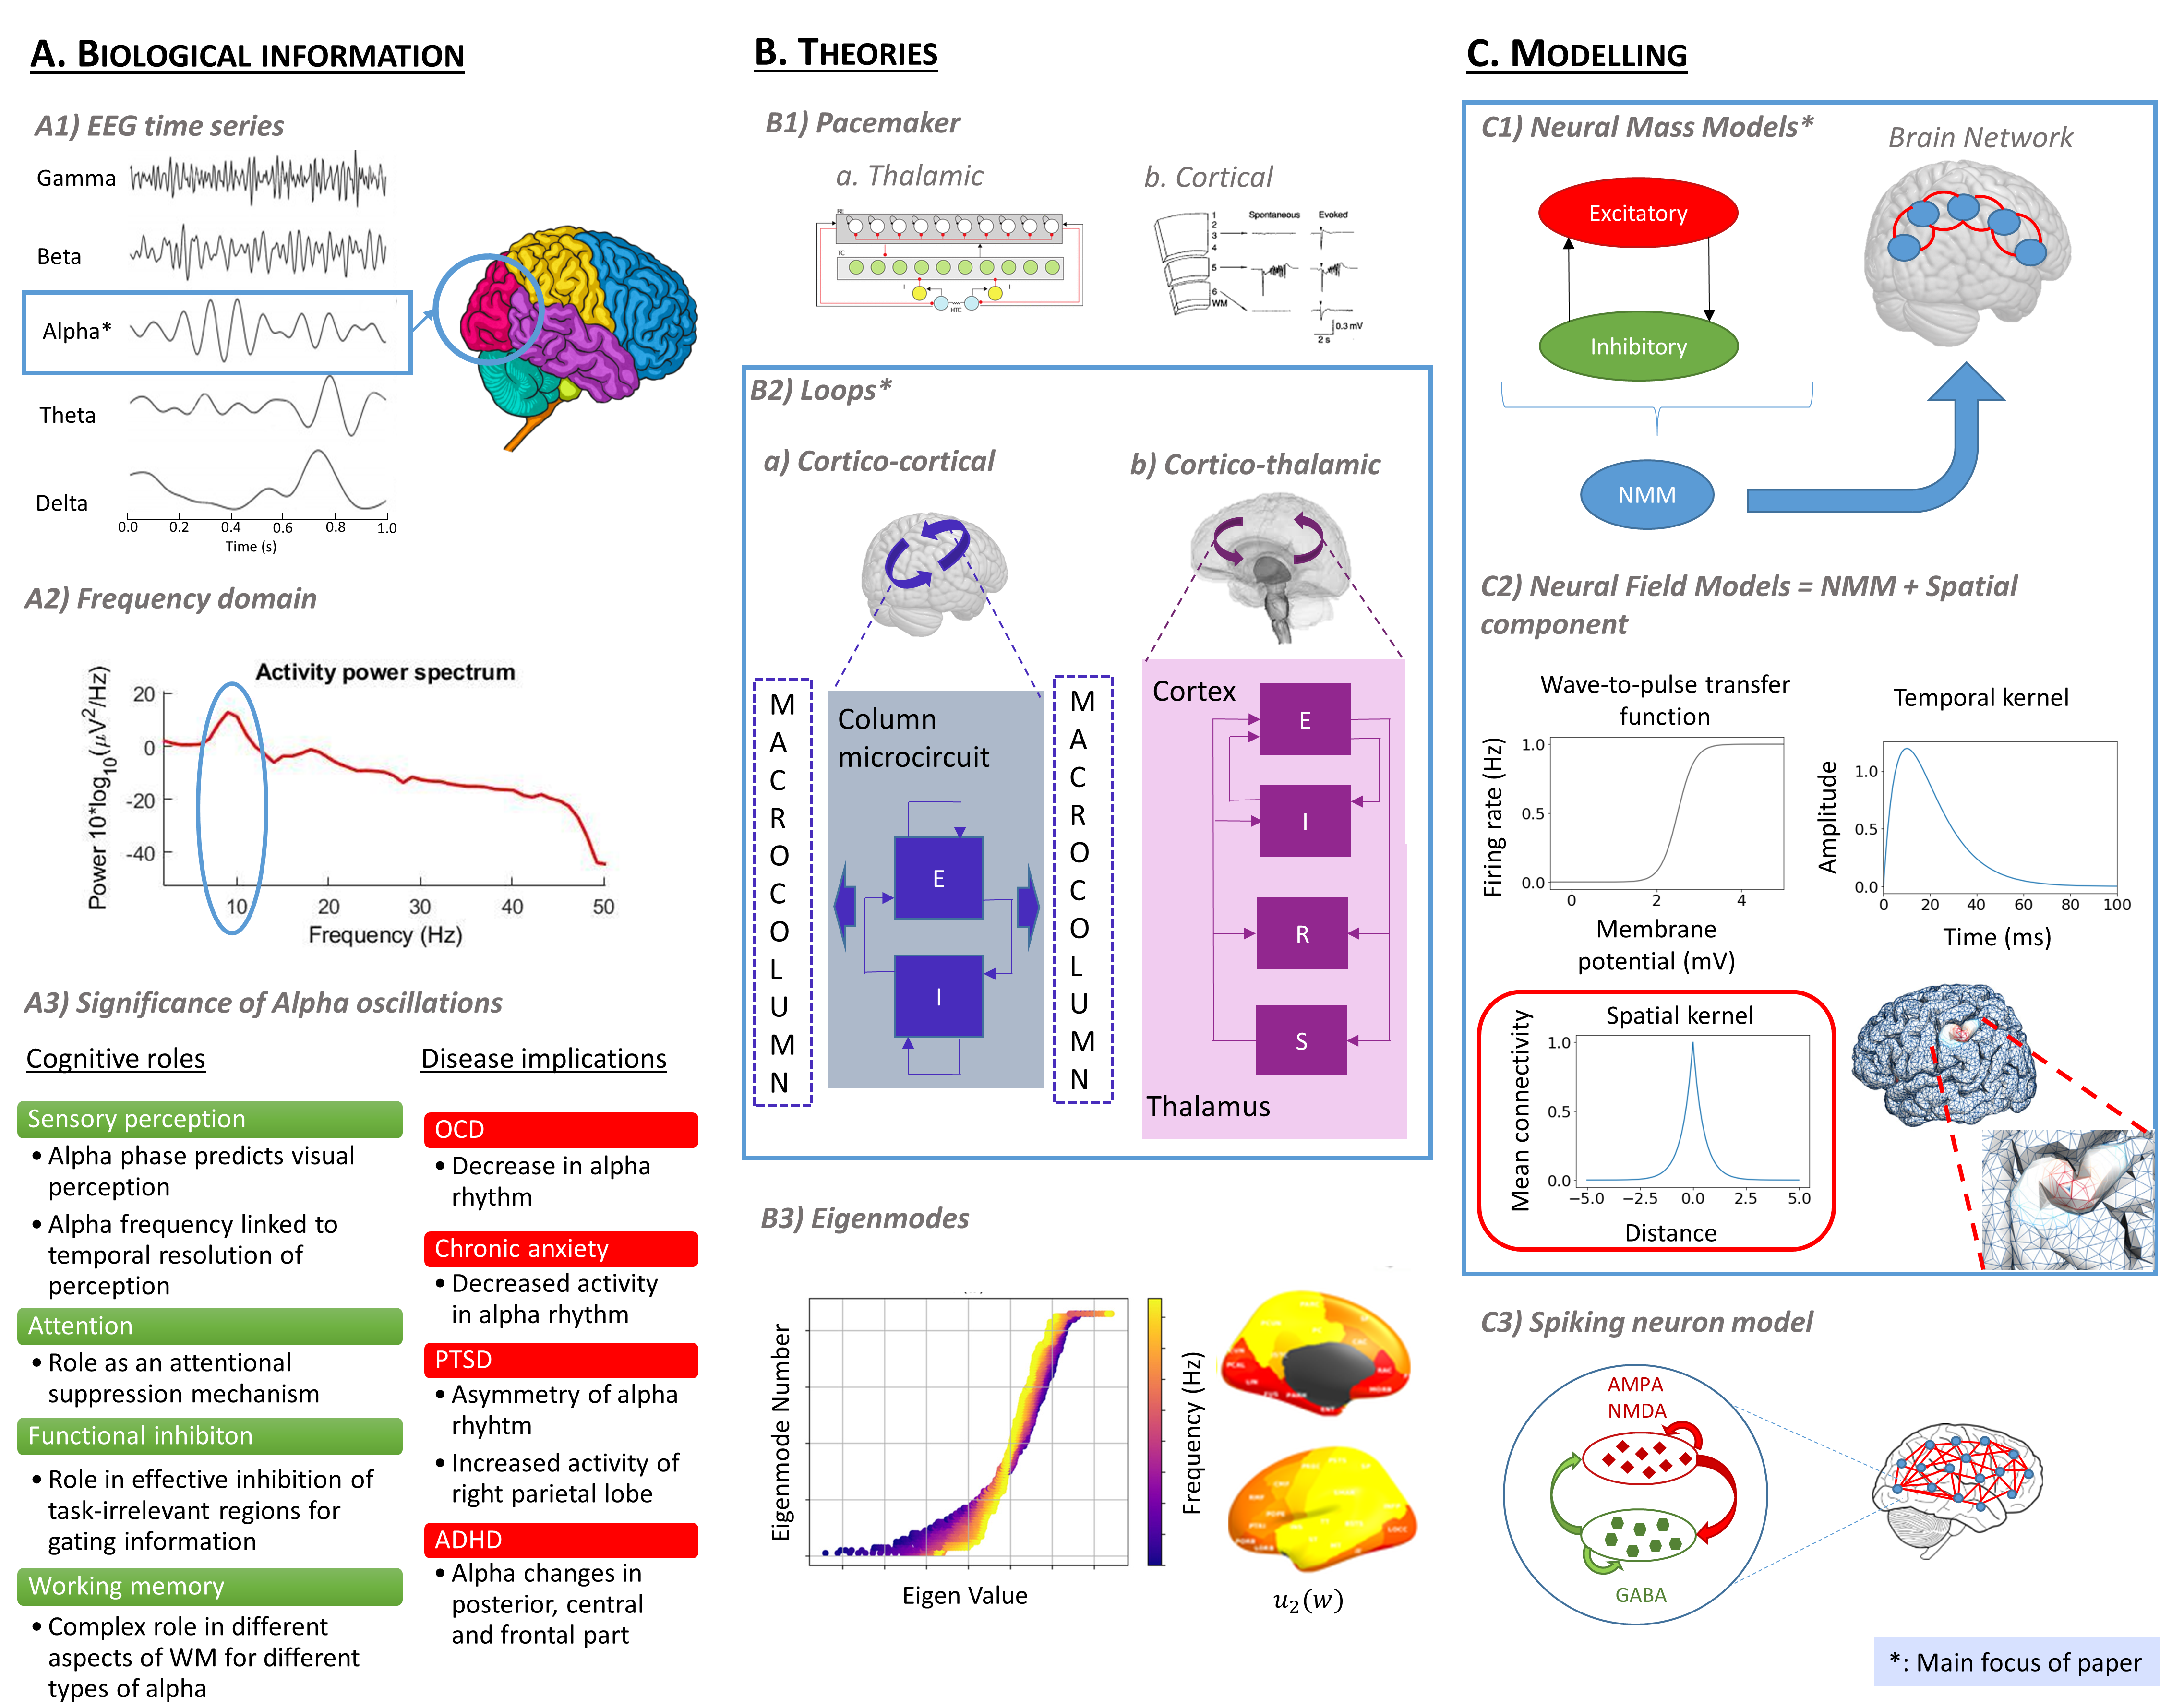
\includegraphics[scale=0.45]{Images/Fig1__Overview_3.png}
    \caption*{\textbf{Figure 1.  \textit{Overview of steps leading to neural population models of alpha oscillations.}} \textbf{A)} Alpha oscillations are most strongly observable in the occipital lobe of the cerebral cortex (A1), where they are characterized by a peak in the power spectrum between 8-12Hz (A2). Panel A3 summarizes the role alpha plays in cognitive processes, as well as abnormal alpha rhythm features observed in various diseases. \textbf{B)} Summary of the different theories that have been proposed to explain the alpha rhythm. We focus on theories emphasizing the importance of interactions between neural populations (B2). \textbf{C)} Alpha rhythm theories are clarified and concretized by mathematical formulations, allowing numerical and analytical investigation of their predictive and explanatory scope. The principal class of models used to date are neural population (neural mass and neural field) models (C1 and C2), which are the focus of the present work.}
    \label{fig:Overview}
\end{figure}
%TC:endignore
%\section{Background} if possible replace intro with background
\subsection{The alpha rhythm: origins and theories}

Neural oscillations are repetitive, quasiperiodic patterns of brain activity that are believed to play a key role in various sensory-cognitive processes \citep{pmid24174901}. In humans, oscillations are most commonly studied with EEG, a non-invasive neuroimaging modality that uses scalp-recording electrodes to capture large-scale neuroelectric activity with high temporal resolution. EEGs measure differences in electrical potential between recording and reference electrodes on the scalp that results from summed postsynaptic dipoles in the brain. In order to quantify oscillatory activity, the measured signal is typically decomposed into its power spectrum frequency components via Fourier transform, and often aggregated into canonical frequency bands (delta: 1-4Hz, theta: 4-8Hz, alpha: 8-12Hz, beta: 12-35Hz, gamma: above 35Hz) for further analysis \citep{ABHANG201619}.

Alpha waves, usually defined as the EEG frequency band between 8 and 12 Hz \citep{MOINI2020177}, are associated with quiet wakefulness, meditation, relaxation and reflection \citep{halgren2019generation}. In the EEG recording, they are most prominent in the occipital lobe of the cortex when the subject is awake with eyes closed  during resting state \citep{klimesch1999eeg}. Their role is believed to be fundamental for a number of top-down cognitive processes \citep{halgren2019generation} such as sensory perception \citep{samaha2015speed}, attention (as an attentional suppression mechanism \citealt{foxe2011role}), functional inhibition \citep{jensen2010shaping} working memory \citep{wianda2019roles} and long-term memory  \citep{klimesch2012alpha}.
Abnormal EEG rhythmic patterns, including aberrant alpha oscillations, are indicative of atypical bioelectrical activity that may suggest the presence of cognitive and/or mental disorders. Thus, robust resting state alpha activity is considered an indicator of healthy cognitive functioning. Reduced alpha power or lowered alpha peak frequencies resulting from aging, head trauma, or exposure to toxins may be correlated with a neurological disorder or brain impairment, such as traumatic brain injury (TBI), or dementia \citep{scally2018resting, buchanan2021elevated}. Both the power and topography of the alpha rhythm is altered in epilepsy patients \citep{abela2019slower}. Several psychiatric conditions are also associated with a decrease in activity in the alpha rhythm, namely chronic anxiety \citep{fingelkurts2006composition, roohi2017changes}, and obsessive compulsive disorder (OCD), sometimes accompanied by concomitant changes at theta and beta frequencies \citep{karadag2003quantitative}. Asymmetry of the alpha rhythm and increased activity of the right parietal lobe is observed in patients experiencing post-traumatic stress disorder (PTSD) \citep{metzger2004ptsd,roohi2017changes}. 
A comprehensive survey of the vast research literature on alpha in cognitive and clinical neuroscience is beyond the scope of the present work; for this we refer the reader to excellent recent treatments by \citet{ippolito2022role, bacsar2012short}

%Even though it was the first rhythmic wave documented and named by Hans Berger in 1929 \citep{berger1929elektroenkephalogramm, tudor2005hans}, and is considered the predominant oscillation in the human brain \citep{klimesch2012alpha} of great importance in terms of their prominence in empirical EEG data, and their implication across a number of clinical and cognitive neuroscience as illustrated previously - the physiological mechanism behind their generation as well as their functional significance remains elusive. 
Although the alpha rhythm was the first rhythmic wave identified and named by Hans Berger in 1929  \citep{berger1929elektroenkephalogramm, tudor2005hans}, and it is considered the predominant oscillation in the human brain \citep{klimesch2012alpha} with significant implications in empirical EEG data and various clinical and cognitive neuroscience studies, the physiological mechanism underlying its generation and functional significance remain poorly understood.
%The complexity is in part due to the likely existence of multiple independent alpha-generating circuits supported by both thalamo-cortical and cortical-cortical loops, since self-sustaining sources have been identified in both regions (layer V of the cortex and thalamus) \citep{nakagawa2014delays}.
%The complexity arises from the probable presence of multiple independent circuits generating alpha waves, which are supported by thalamo-cortical and cortical-cortical loops. Self-sustaining sources have been identified in both regions, namely the thalamus and layer V of the cortex \citep{nakagawa2014delays}. 
Unlike other characterized brain oscillations, such as beta and gamma waves, whose neural circuitry relies on local connectivity \citep{lozano2018physiological}, the generation of alpha rhythm is thought to involve contributions from both cortical and thalamic regions, which can influence and interfere with each other, suggesting an elaborate neural circuitry \citep{lozano2018physiological,da1991neural}. Several hypotheses have been proposed regarding the composition and mechanistic organization of these alpha circuits, which can be grouped under three categories: \textit{pacemaker}, \textit{local network}, and \textit{global network} theories. The pacemaker theory suggests that intrinsic alpha oscillations are generated either in the thalamus, driven by pulvinar or and/or the lateral geniculate nucleus \citep{saalmann2012pulvinar, lHorincz2009temporal, hughes2011thalamic} or in the cortex, originating from the pyramidal cells located in layer V \citep{da1991neural, connors1997making, bollimunta2008neuronal}. However, pacemaker theories in general suffer from several severe limitations (see \citealt{nunez2006electric} for an extensive discussion of this). For instance, pacemaker cells such as putative thalamic nuclei, if they exist, would have to function in a relatively autonomous fashion, having a highly restricted input from other oscillatory brain regions - a notion that has been critically questioned on anatomical grounds \citep{lopes1998dynamics, steriade2005cellular}. Additionally, there are certain global EEG phenomena that remain unexplained, including the relative frequencies of major rhythms and sleep-wave variations. The second category, `local network' theories,  propose that alpha rhythms are produced by interactions between excitatory and inhibitory neural populations with dendritic response functions and saturating nonlinearities \citep{valdes2010white}. Finally, `global network' theories posit that alpha rhythms are generated by large-scale networks rather than local circuits within a localized brain region. %large-scale networks 
By disregarding complex dendritic response functions and finite intracortical propagation, models with a primary emphasis on global dynamics rely heavily on the propagation delays between distant anatomical structures to shape their dynamics \citep{nunez1995neocortical, nunez2006theoretical, valdes2010white}. Of these three categories, local network theories are the most established and extensively studied, and will serve as the major emphasis in the present work. Specifically, we examine in detail two prevailing local network theories of alpha rhythmogenesis: 

\begin{enumerate}

\item   Alpha oscillations are generated by recurrent activity and excitatory-inhibitory interactions within cortical column microcircuits.%[source]

\item	Alpha oscillations are generated by delayed inhibitory feedback within corticothalamocortical loops.   %[source]

%\item   The harmonic eigenmode structure of large-scale cortico-cortical networks is a core determinant of the 8-13Hz characteristic frequency range.% [source]

%\item   Thalamic and cortical pacemaker neurons are responsible for the generation of the alpha waves. %[source]

\end{enumerate}

These two accounts describe the origin of alpha waves as a phenomenon relying on dynamics of local networks of interconnected neural populations, and thus occurring at the \textit{mesoscopic} spatial scale. Computations underlying brain functions such as action, perception, learning, language and higher cognition are hypothesized by some to operate from neural ensembles at this scale \citep{deco2008dynamic}. Current technologies allow us to measure the macroscale (EEG, MEG, fMRI, ECoG) or the microscale (single cell recording, fluorescence calcium imaging, multielectrode arrays), but the mesoscopic scale is more challenging to directly observe, particularly in humans \textit{in vivo}. To bridge the gap between scales and explore the underlying mechanisms of alpha rhythmogenesis, mathematical models of neural networks replicating EEG phenomena observed empirically are particularly useful. The class of computational neural models that simulate neural activity directly at the mesoscopic level are known as neural population models (NPMs). %stronger transition
%TC:ignore
\begin{figure}[H]
    \centering
    %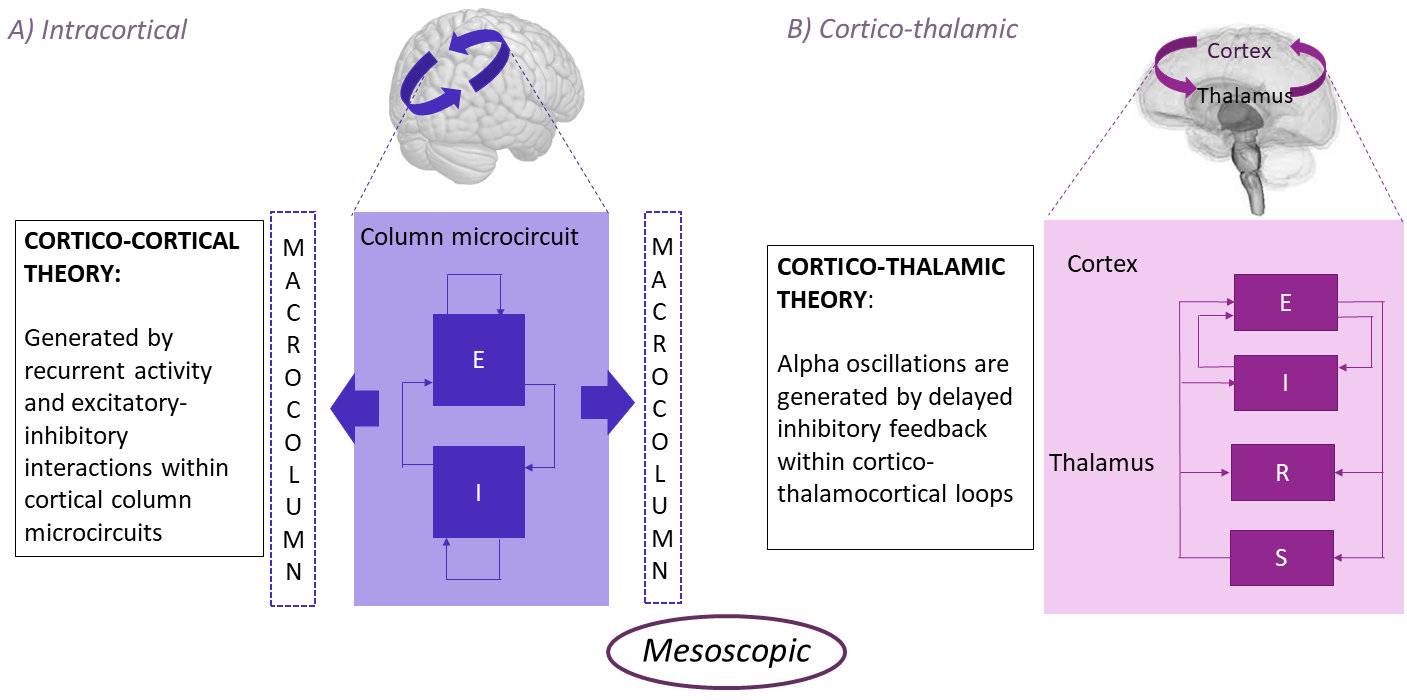
\includegraphics[scale=0.45]{Images/Figure2_theories.png}
    %\caption*{\textbf{Figure 2.  \textit{ Schematic depiction of the two main theories focused on local neural population connectivity to explain alpha rhythmogenesis from which mathematical models are built.}} \textbf{A)} Cortico-cortical model which consists of interconnected macrocolumns each composed of excitatory and inhibitory neural populations. \textbf{B)} Cortico-thalamic model which includes neural populations of the thalamus in the process of alpha genesis.}
    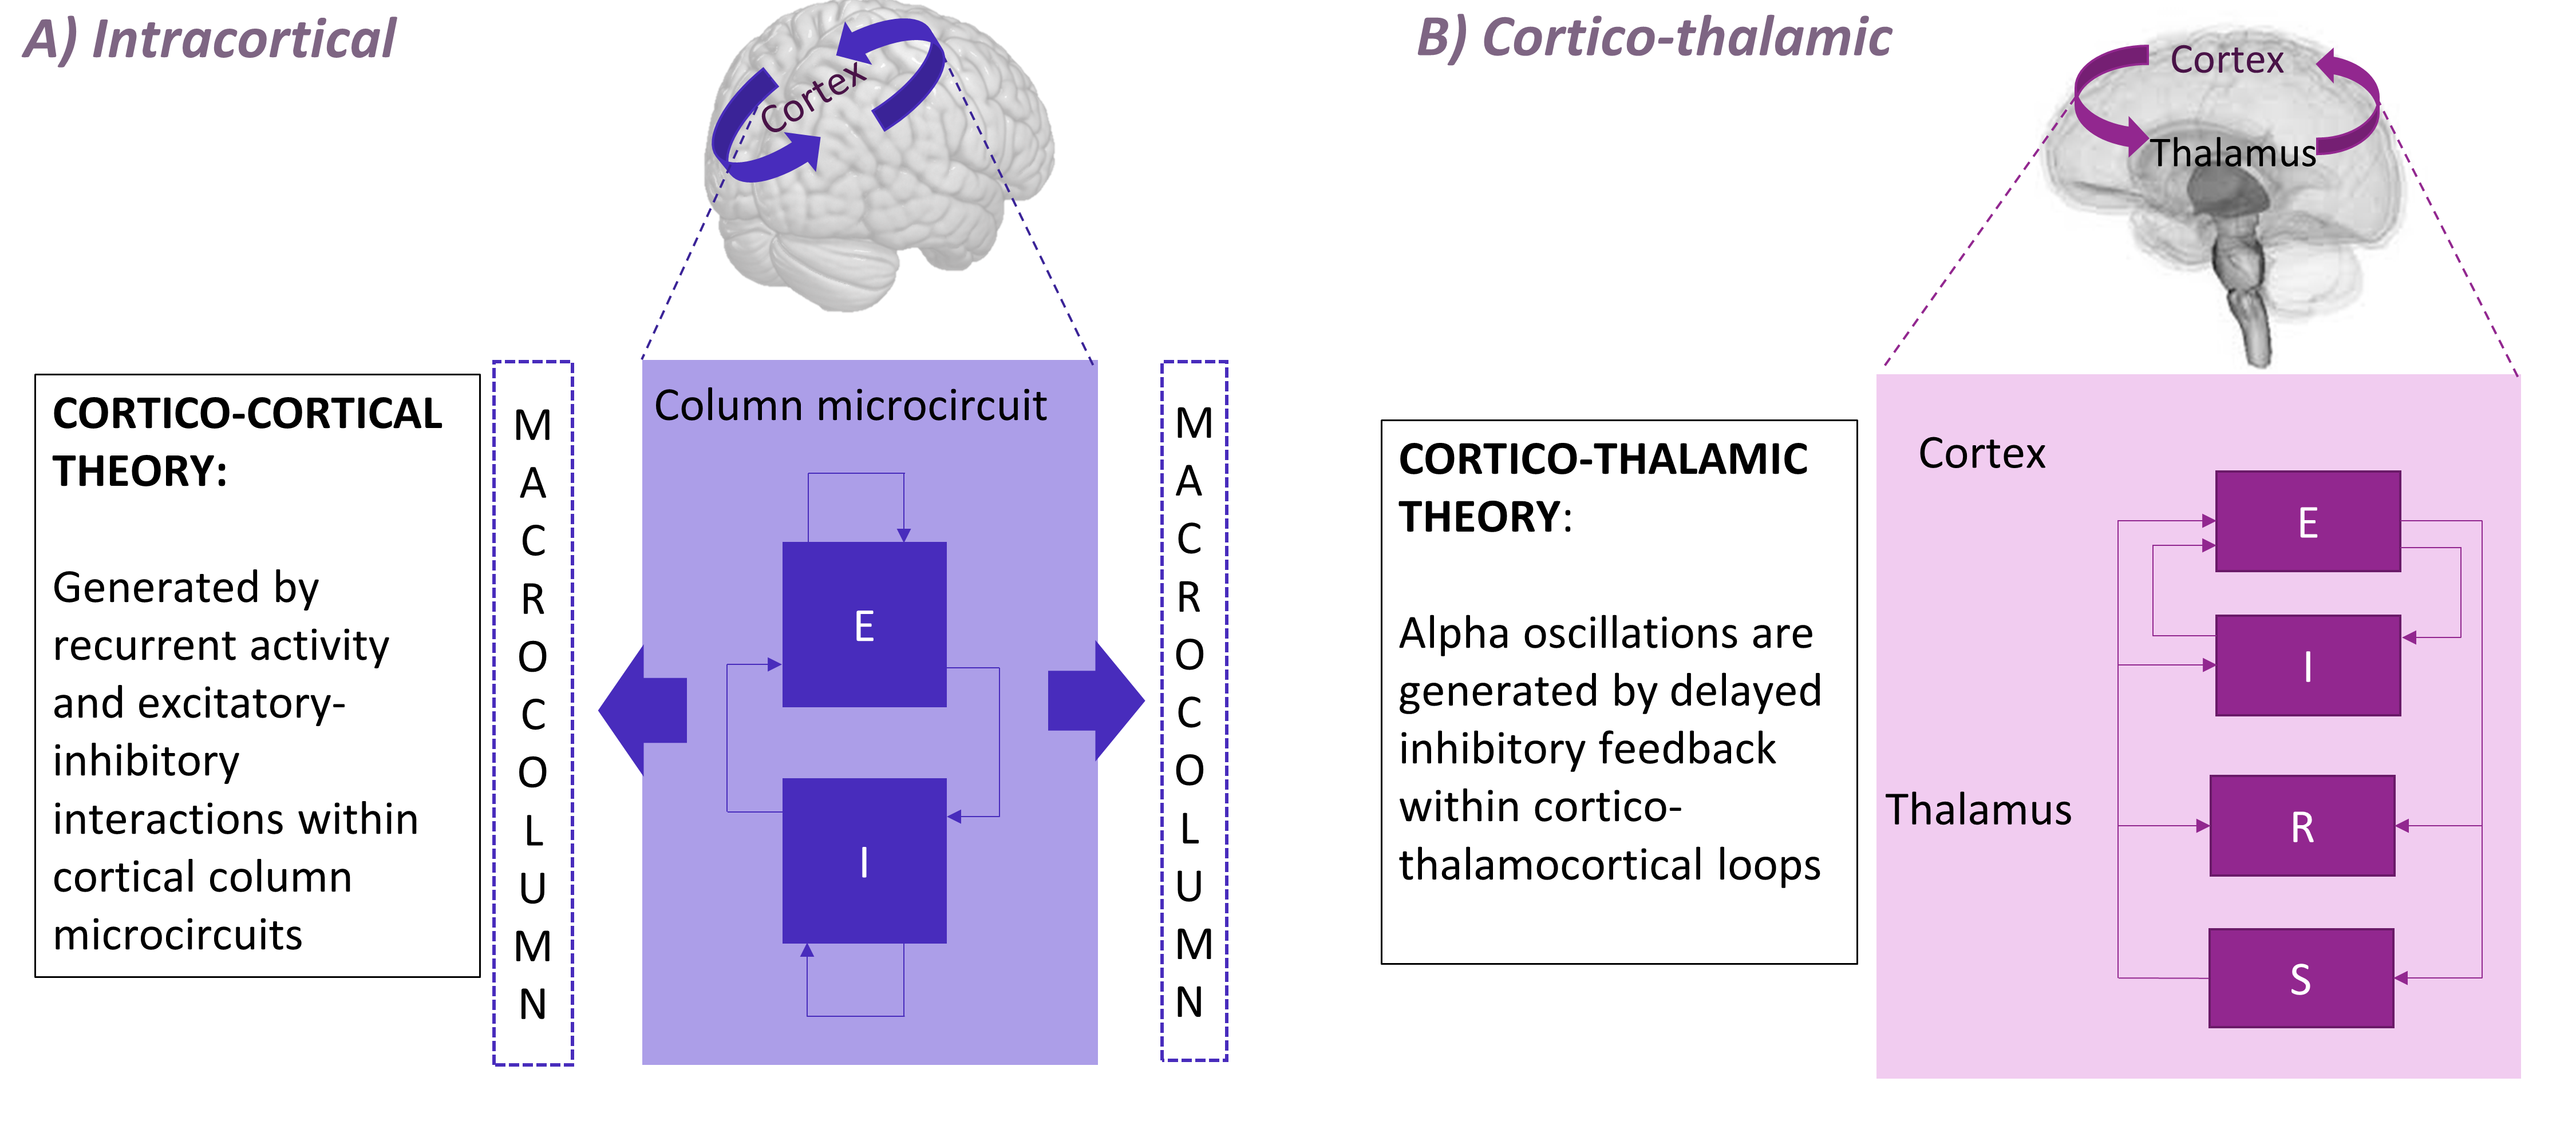
\includegraphics[scale=0.45]{Images/Fig2__Theories.png}
    \caption*{\textbf{Figure 2. \textit{Schematic depiction of two candidate theories of alpha rhythmogenesis.}} \textbf{A)} Cortico-cortical columnar microcircuit model, representing the generation of alpha rhythm through interconnected macrocolumns. \textbf{B)} Cortico-thalamic model, involving thalamic neural populations in the process of alpha genesis.}
    \label{fig:Theories}
\end{figure}

%\subsection{Mathematical models of neural population dynamics}
\subsection{Bridging scales: mathematical modelling of mesoscopic neural population dynamics}
%TC:endignore
Mathematical expressions of human brain activity have provided significant insights into the hidden mechanisms of the underlying neural processes at multiple scales \citep{deco2008dynamic}. To construct models at the intended level of granularity, there are two main approaches: 1) a `bottom-up' approach, beginning at the sub-cellular level with flows of ions and action potential generation at small patches of neuronal membrane (typically using Hodgkin-Huxley or Rall model equations), or at the whole-cell level (e.g. using Izhikevich or Leaky Integrate-and-Fire model equations); or 2) a `top-down' approach, which represents the collective activity of neurons sharing some common characteristics, such as the type of synapses they connect to (excitatory or inhibitory) instead of focusing on individual cells \citep{cook2021neural, cooray2023global}. While the former approach is a closer representation of biological neurons with finer details, it is often inadequate for modelling empirical phenomena emerging from large-scale brain activity, as the complexity rapidly increases with the number of neurons involved, resulting in interpretability and computational issues \citep{cook2021neural}. Since our investigation focuses on the alpha rhythm, we prioritize models that take a `top-down' approach in our study, and provide a systems-level perspective which can give a more holistic understanding of alpha rhythm and its functional significance.

%This top-down perspective is based on the neural ensemble approach \citep{breakspear2017dynamic}, which assumes that at large spatial scales the activity of each individual neuron is negligible compared to the global activity of a segregated neural population with a common type of synaptic connectivity (i.e `excitatory' or `inhibitory'), and the states of neurons across the ensemble are uncorrelated. 
The top-down perspective, based on the concept of neural ensemble dynamics \citep{breakspear2017dynamic}, assumes that the activity of each individual neuron is negligible at large spatial scales. Instead, the aggregate activity of a population of neurons with a common type of synaptic connectivity (i.e. excitatory or inhibitory) is considered, and the states of neurons across the ensemble are assumed to be uncorrelated. This approach, which is followed by all NPMs, is particularly useful for modelling oscillatory activity such as the alpha rhythm, since the spatial scales of the variables are equivalent to the physical coverage of an individual EEG channel (mm$^2$ - cm$^2$) and so can be understood as approximating local field potentials \citep{coombes2014neural, evertz2022alpha}. 

NPMs therefore represent a mesoscale formulation that aims to capture the emergent properties of collective activity within a patch of neural tissue. In the literature, the term NPM is used with varying interpretations. In our context, NPMs encompass a range of large-scale computational models namely neural mass models, mean-field models, and neural field models \citep{deco2008dynamic, bojak2014neural}. 
Models following the ensemble approach can be further reduced by assuming a diffusion approximation \citep{coombes2019next,deco2008dynamic}. In this formulation, the neural population activity is then defined as a standard normal probability distribution, and is completely characterized by the mean and variance of the firing rate \citep{breakspear2017dynamic}. Dynamics expressed as a linear, normally distributed ensemble can be described using the Fokker-Planck equations. For a more detailed description of these equations and models of large-scale brain dynamics, we refer the reader to \citet{breakspear2017dynamic}. 
% From spiegler if want more details on Fokker-plank in main text: NMMs are a special case of the ensemble density approach which are in line with both state reduction and approximation. Here, the ensemble dynamics with all their diversities are reduced to an averaged neural state of a neural ensemble such as mean firing rate or mean mem brane potential (i. e., expectation values of densities). Thus, NMMs are parsimonious in terms of parameters and suitable for parameter study and for system inversions of given data like that of M/EEG [50]. The main impact of this reduction is that it enables the states to be coupled simply by the expectation (i. e., first moment) of a state, while the Fokker-Planck formalism permits coupling of each statistical moment of a probability density within and between neural ensembles. Finally, the Fokker-Planck formalism explicitly shows the variability of a state, whereas the reduced NMMs only features variability implicitly (i. e., slope of the sigmoidal transfer function [140–142]). The interested reader will find more on this general subject in the excellent papers about density models [4,130] and the citations therein. What is dealt with in the present work is NMMs, and the following subsection introduces the concept and the related mathematics.
%By using the Fokker-Planck equations, the collective neural activity can be described by the mean and variance of the firing rate. 
If strong coherence is assumed between neurons, the activity of the ensemble is sufficiently close to the mean that the variance becomes fixed, reducing the number of dimensions. NMMs can be understood as a special case of the Fokker-Planck equations where the variance is fixed, and the mean remains variable. They are then able to represent the coarse-grained activity of large populations of neurons and synapses with a small number of equations \citep{jansen1995electroencephalogram, lopes1974model, breakspear2017dynamic}. NMMs are the simplest type of NPM capable of describing the change in firing rate of neural populations without spatial information and spatiotemporal time delays, providing a succinct yet biophysically meaningful description of brain activity at the mesoscopic scale \citep{spiegler2012dynamics, cook2021neural}. The main advantage of NMMs is that the simplification of the dynamics reduces the number of dimensions or differential equations that need to be integrated, enabling us to hone in on the behavior of a large number of ensembles and more clearly understand their dynamics \citep{deco2008dynamic}. Furthermore, complex systems may exhibit emergent behavior that cannot be explained solely by the behavior of individual components, but rather arises from the collective interactions and relationships among them \citep{breakspear2017dynamic}. Thus, rules governing the behavior of a complex system may differ from those at lower levels of organization, as the system as a whole can be more than the sum of its individual parts \citep{moran2011vivo}. The aim is to propose a model that is balanced between mathematical tractability and biological plausibility \citep{spiegler2012dynamics}.

Since NMMs assume a point mass, they evolve in time but not in space, unlike neural field models (NFMs) which include a spatial component by considering the cortex as smooth sheet, supporting waves of propagating activity \citep{pinotsis2014neural, breakspear2017dynamic} usually expressed in the form of a damped wave equation allowing the description of the activity over the entire cortex. When spatial uniformity is assumed in a NFM, the model can be likened to a NMM. Simulation of whole-brain activity with NMMs can also be achieved by coupling neural masses according to a weighted connectivity matrix representing the strength of the anatomical connections, known as the connectome, often estimated with diffusion-weighted MRI data \citep{breakspear2017dynamic, schirner2018inferring, glomb2021computational}. Each node corresponds to a NMM depicting a brain region to collectively form an integrated brain network model. 

Alpha oscillations have been successfully simulated with both NPM (NMM and NFM) and have been studied to shed light on the complex dynamics of neural systems. In the following paragraph, we discuss early pioneers of NMMs and NFMs who have greatly influenced current models in terms of structure, parameter values, and implementation. 
%\subsubsection{Pre-history of neural population models}

%TC:ignore
\subsection{Tracing the roots of NPMs: early history}
%TC:endignore
The notion of neural \textit{masses} was introduced in various forms 
during the 1950s and 1960s \citep{beurle1956properties, griffith1963field}, and consolidated in the 1970s primarily through the highly influential work of Freeman, Wilson \& Cowan, Amari, and Nunez. It was Freeman who originally used the term `neural mass action model' \citep{freeman1972linear, freeman1972waves, freeman1975mass}, articulating many of the neurobiological and mathematical fundamentals as they are understood today in a wide-reaching monograph on the subject \citep{freeman1975mass}. Here, Freeman also %expands/explains/
develops the theory of `K-sets' which are based on a hierarchy of interacting sets of neural populations or masses, and used to model neural population dynamics with ordinary differential equations (ODEs) to simulate mesoscopic local field potentials \citep{deschle2021validity}. The levels are designated as K0, KI, KII, and KIII, with the K0 set corresponding to a model characterized by non-interactive collections of neurons with globally common inputs and outputs, KI to pairs of interacting K0 sets, and so on. Freeman's research on the olfactory bulb and prepyriform cortex of cats and rabbits \citep{freeman1979nonlinear, freeman1975mass} provides valuable experimental data that has been used to define mathematical formulations and parameter settings in many NMMs, which is further discussed in section 3.2.4. Furthermore, Freeman's contributions on the use of the sigmoidal operator for mapping membrane potential to firing rate remains a critical component of many NMMs, the validity of which will be elaborated on in section 4.2. Even though Freeman coined the term neural masses and laid much of the groundwork, many of the core mathematical principles of NMMs were first proposed in the work of Wilson \& Cowan (WC; \citealp{wilson1972excitatory}), which itself builds upon earlier work by \citet{beurle1956properties}. WC's implementation introduced and solidified an approach to modelling neural dynamics and brain function. This approach consists of analyzing the collective properties of a large number of neurons using methods from statistical mechanics rooted in the mean-field framework \citep{destexhe2009wilson,chow2020before}. By omitting potential spatial arrangement of synaptic connections, their model offers a minimalistic NMM representation that has been leveraged to develop several simple yet biophysically plausible models (eg \citealp{Kilpatrick2013, sanz2015mathematical}). As shown in Fig. 3, the canonical WC model consists of two neural masses with one excitatory and one inhibitory population \citep{wilson1972excitatory,sanz2015mathematical}. Two nonlinear ODEs describe the dynamics of those two synaptically coupled populations in the neocortex \citep{nakagawa2014delays,cowan2016wilson}. The WC system is thus a coarse-grained description of the overall activity and mesoscale neuronal network structure of a patch of (usually cortical) tissue, as is typical of NPMs. By varying the connectivity strength and the input strength to each population, it is possible to generate a diversity of dynamical behaviors that are characteristic of observed activity in the brain, such as multistability, oscillations, traveling waves, and spatial patterns \citep{Kilpatrick2013}. 
%TC:ignore
\begin{figure}[h]
    \centering
    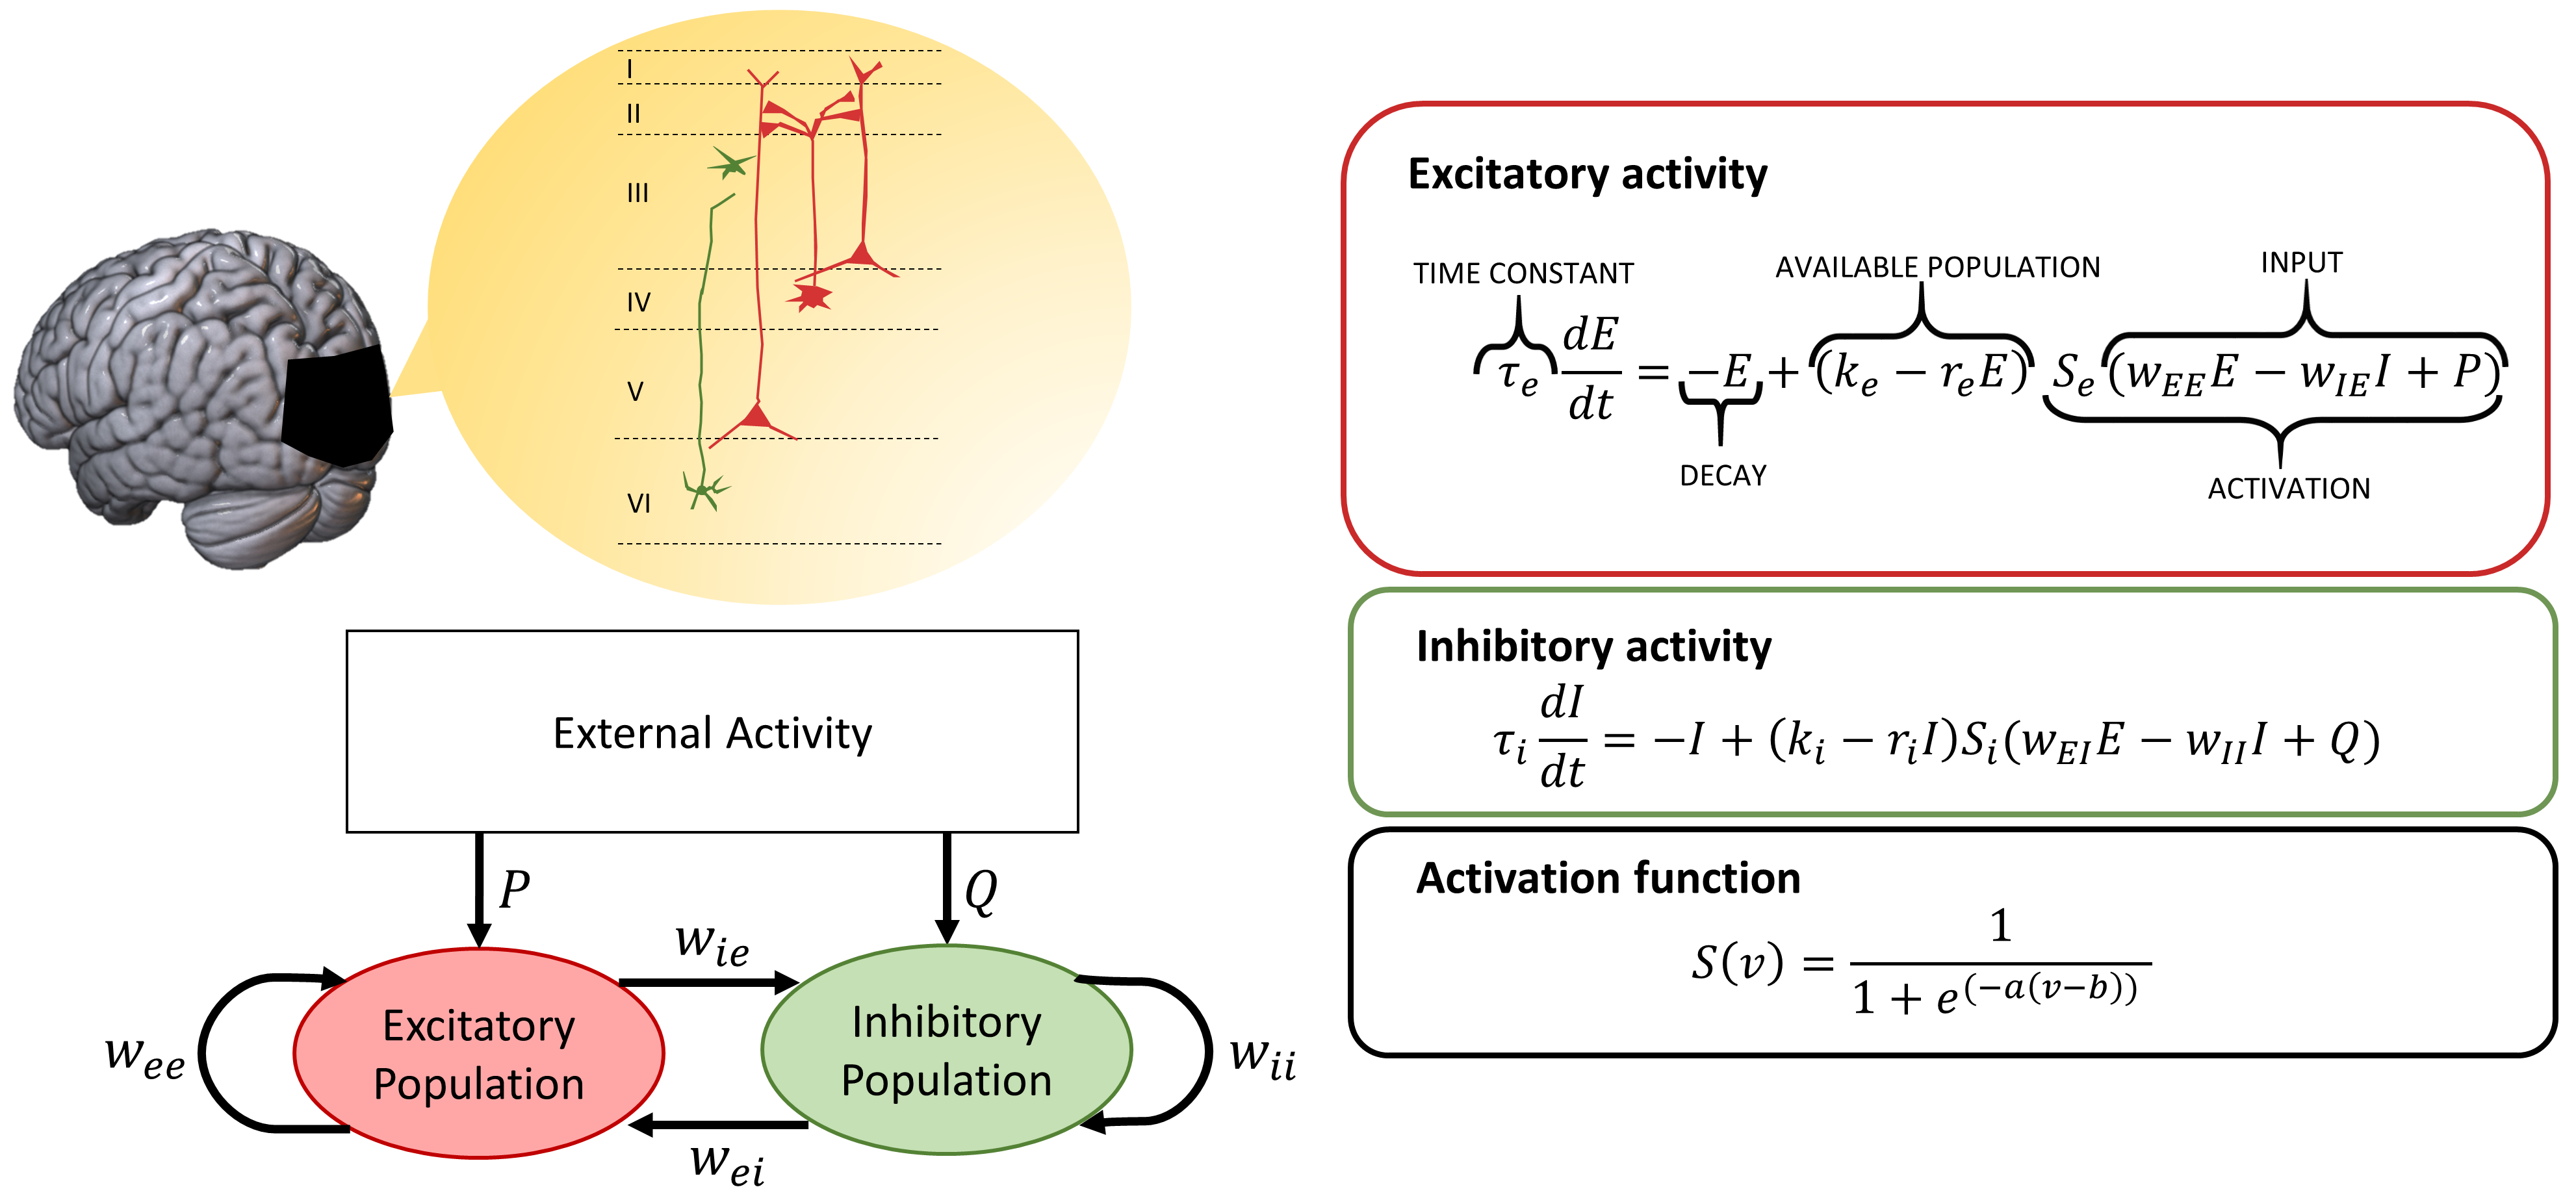
\includegraphics[scale=0.48]{Images/Fig3__WC.png}
    \caption*{\textbf{Figure 3.  \textit{Wilson-Cowan model topography and mathematical expression}}. The model aims to represent a cortical column within the brain, consisting of an excitatory and an inhibitory population. These two connected populations each have a self-connection and external activity as input. Dynamics are expressed with nonlinear ordinary differential equations which are shown on the right for each neural population. Nonlinearity is introduced with the sigmoidal operator corresponding to the activation function.}
    \label{fig:WC_topography}
\end{figure}
%TC:endignore
%\begin{figure}[H]
 %   \centering
  %  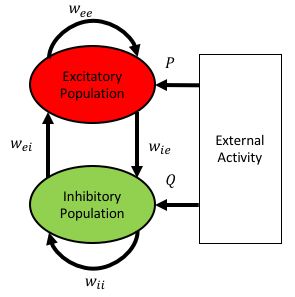
\includegraphics[scale=0.5]{Images/WC_Topography.png}
   % 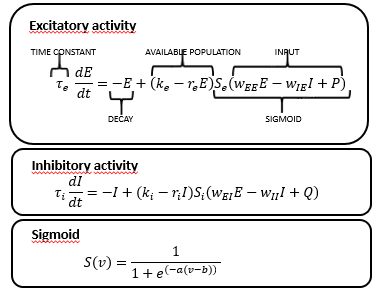
\includegraphics[scale=0.75]{Images/WC_equations.png}
    %\caption*{\textbf{Figure 2.  \textit{Wilson-Cowan model topography and mathematical expression}}. Add description.}
    %\label{fig:WC_topography}
%\end{figure}

%Mathematical equations
%Sigmoid:
%\begin{equation}
 %   S(v)=\frac{1}{1+e^{-a(v-b)}}  )
%\end{equation}
%Excitatory activity:
%\begin{equation}
 %   \tau_e \frac{dE}{dt} = -E+(k_e-r_e E) S_e (w_{EE} E-w_{IE} I+P)
%\end{equation}
%Inhibitory activity:
%\begin{equation}
 %   \tau_i \frac{dI}{dt} = -I+(k_i-r_i I) S_i (w_{EI} E-w_{II} I+Q)
%\end{equation}

%(see presentation slides for details on each elements)

A simplified version of the WC equations shown in Fig. 3 has been previously implemented by \citet{abeysuriya2018biophysical} in a network of neural masses to generate alpha oscillations. These two populations are described as follows:

\begin{eqnarray}
    \tau_{e}\frac{dE(t)}{dt} &=& -E(t) + S(w_{ee}E(t) + w_{ie}I(t) + P + \epsilon(t)) \\
    \tau_{i}\frac{dI(t)}{dt} &=& -I(t) + S(w_{ei}E(t) + \epsilon(t))
\end{eqnarray}

where $E$ and $I$ represent the activity of the excitatory and inhibitory neural populations in the form of mean firing rates, $\tau_{e/i}$ are the excitatory/inhibitory time constants, $w_{ab}$ are the local connection strengths from population $a$ to population $b$, $P$ is a constant external input to the excitatory neural population, and $\epsilon$ is a noise signal added to the system. The studied NMMs share similar parameters, with some variations such as the use of membrane potential instead of firing rates as the state variable, and the concatenation of the external input and noise term into a single variable.

Concurrently to WC and Freeman, Lopes da Silva and colleagues developed a point-process model of EEG alpha rhythm generated with a corticothalamic loop \citep{lopes1974model}. Specifically, these authors proposed a negative feedback loop between excitatory thalamocortical relay cells and inhibitory thalamic reticular neurons as the basis for generating certain brain rhythms, in a manner similar to the interacting E and I populations in the WC model. By applying linear systems analysis to investigate the influence of physiological parameters on neural periodic patterns, they established a novel approach to studying oscillatory dynamics in theoretical neuroscience that relied on analytical power spectra.
%Linear system analysis was used to understand the effects of the physiological parameters analytically \citep{lopes1974model}, and as such was one of the first times in theoretical neuroscience of an analytic power spectrum being used to study oscillatory neural dynamics. 
The Lopes da Silva model had a substantial impact on subsequent corticothalamic models and linear analysis tools \citep{cona2014thalamo,bhattacharya2011thalamo}.

A few years later, \citet{zetterberg1978performance} %(NOTE: MIGHT BE 1973, can't seem to find this paper),
built an extension of the model by adding a second cortical excitatory population in order to separately account for pyramidal cells and excitatory interneurons. Their work was then reprised and further popularized by \citet{jansen1995electroencephalogram}. In the JR model, each neural population is described in two steps: a transformation of the incoming average pulse density of action potentials into an average postsynaptic membrane potential, followed by a sigmoidal function to perform the inverse conversion. Over the years, several extended versions of JR have been proposed \citep{wendling2000relevance, david2003neural, zavaglia2006neural, sotero2007realistically}, - including Moran et al., where they focused on steady-state spectral responses with a linearized approximation of the model \citep{moran2007neural}. Contemporaneous with these early conceptualizations and formulations of NMMs in the 1970s was the introduction of NFMs by Amari, Wilson \& Cowan, Nunez, and others. The `brain wave equation' model of \citep{nunez1974brain} is particularly important here as it was the first to attempt to describe neural activity across the entire cerebral cortex with an evolution in both time and space. This work was a major influence for several macroscale NFM formulations in the 1990s \citep{jirsa1996field, wright1996dynamics, robinson1997propagation}. The latter of these which was then extended in 2001 to include the thalamus, and subsequently used to investigate a wide range of brain states including sleep \citep{robinson2005multiscale, abeysuriya2014prediction}, epileptic seizures \citep{zhao2015generalized, breakspear2006unifying}, evoked responses \citep{kerr2008physiology}, functional connectivity \citep{robinson2014determination}, and alpha rhythms \citep{robinson2002dynamics, robinson2005multiscale}.

For a more detailed timeline and review on the development of NPMs and whole brain modelling in general, we refer the reader to \citet{griffiths2022whole} and \citet{chow2020before}. The early mathematical models reviewed there and above laid the groundwork for most NPM formulations used in theoretical neuroscience today. In particular, they form the basis for the four most widely studied models of the EEG alpha rhythm - Jansen-Rit (JR), Moran-David-Friston (MDF), Liley-Wright (LW) and Robinson-Rennie-Wright (RRW). Before presenting each of these models individually in detail, we conclude our background review in the next section by examining the two common mathematical operators of NPMs.

%TC:ignore
\subsection{Classification of NPMs and mathematical characteristics of \\ convolution-based models}
%TC:endignore
NPMs can be further divided based on different modelling approaches, including convolution vs. conductance-based models and voltage vs. activity-based models. For conductance-based models, very high coherence between neurons is assumed, to the extent that the dynamics of neuron population resembles the dynamics of each single neuron. The mathematical equations then follow the same structure as single neuron conductance-based models \citep{marreiros2010dynamic,breakspear2017dynamic}. Since distinct types of ionic currents are explicitly modelled, a direct relationship between modelled synaptic processes and physiological mechanisms can be determined \citep{moran2011vivo}. In contrast, convolution-based NPMs rely on empirical observations of the collective response of a neural population to their inputs, to build a phenomenological model that captures the system's response. 
%This is to take into account the fact that complex systems might present rules that differ from other levels of organizations, as they may be more than the sum of its parts \citep{moran2011vivo}. 
%This is to take into account the fact that complex systems may exhibit emergent behavior that cannot be explained solely by the behavior of individual components, but rather arises from the collective interactions and relationships among them. Thus, rules governing the behavior of a complex system may differ from those at lower levels of organization, as the system as a whole can be more than the sum of its individual parts \citep{moran2011vivo}. 
Although convolution-based models lack the biological detail of conductance-based models, they provide a more straightforward and interpretable framework for understanding the system-level dynamics of neural populations.

Since the four models reviewed in this paper are considered convolution-based models, each with slightly different expressions or additional elements, we will present the common mathematical foundations between all of them (which is composed of two operators) allowing for relevant comparisons. Even though a conductance-based model is not explicitly investigated here, we note that the LW model incorporates conductance-based components which enables us to determine how these factors affect the dynamics of the model. %better transiton maybe here

%\vspace{-2.5cm}
The mathematical expression of convolution-based NPMs is composed of two key operators: a rate-to-potential operator describing the dynamics between synapses and dendritic trees, and a potential-to-rate operator representing the output firing rate produced at the soma, which were briefly introduced in the description of the WC equations (Figure 3). The rate-to-potential operator describes a conversion from firing rate to membrane potential by excitatory and inhibitory neurotransmitters, usually in the form of an impulse response. It has been shown that the convolution of the incoming spike rate with an impulse response adequately reproduces the postsynaptic potential in response to presynaptic firing \citep{bhattacharya2013implementing}. This is expressed as a second-order differential equation, which makes the representation of chemical synapses linear \citep{rall1962electrophysiology, rall1964theoretical, freeman1975mass,spiegler2012dynamics}. The nonlinearity is introduced with the potential-to-rate 
operator (also known as a wave-to-pulse conversion \citep{freeman1992tutorial, cook2021neural}), generally in the form of a sigmoid, which transforms the average membrane potential of the population into the average rate of action potentials fired by the neurons. The sigmoid form is not derived from a biophysical model, but rather seen as a physiologically consistent choice \citep{coombes2019next}. Furthermore, the introduction of nonlinearity allows for the representation of more complex behavior (such as chaos) within the brain. It is worth noting that the sigmoidal shape of the function limits the effective dynamic range \citep{spiegler2012dynamics} - the validity of which we discuss further in section 4.2.
Thus the central part of all neural populations in convolution-based NPMs is described by a second-order nonlinear ordinary differential equation, which can either be deterministic or stochastic depending on the external input (usually noise) introduced to the model. NMMs can be further categorized based on the nature of their state variable. In some models, such as WC, the state variable represents the proportion of cells that are active in the population at a given time, referred to as activity-based. On the other hand, in voltage-based models, the state variable corresponds to the membrane potential of the neurons in the population. This means that changes in the state parameters represent changes in the electrical potentials \citep{griffiths2022whole}. Therefore, NMMs are classified based on the mathematical operators used and the biological representation of the output state variable.

% from liley 2001: Most typically these equations describe the spatiotemporal evolution of a time-averaged mean firing rate for each of the neuronal sub-populations.This type of model is referred to as an activity-based model [30] and implicitly assumes that the characteristic timescales of neurotransmitter kinetics are significantly longer than the timescales associated with the passive properties (i.e. the membrane time constant) of the neuron. In the obverse case, when the membrane time constant is much larger than the timescales associated with neurotransmitter kinetics, these mean field models can be reformulated as voltage-based models. In this case the equations describe the spatio-temporal evolution of a time-averaged mean soma membrane potential.

%The nature of the state variable can be different between the models. When the state variable corresponds to membrane potential the model is said to be `voltage-based', whereas if the time-dependent activity variable(s) represent a proportion of cells in the population that are active (i.e. firing) per unit time such as seen in the WC, the model is considered as `activity-based' \citep{griffiths2022whole}.

Almost all convolution-based NPMs in the literature are built upon the presented mathematical operators, which form the fundamental basis of these models. This allows for meaningful comparisons between models, and the impact of varying model elements on the output can be assessed. It is worth noting that these models can be linearized around their stable points, yielding analytic versions of the model equations. Although many assumptions are made, stability analysis has been useful in understanding the dynamics of the systems in question and their implications for brain organization. 
%The two mathematical operators presented, form the backbone of almost all NPM models in the literature, implying that meaningful comparisons can be made between them in order to assess how the varying elements affect the output. 
Even though they share the same backbone, there are three key factors that distinguish the models: 1) the number of neural population modelled, 2) the degree of physiological complexity associated with each neural population, and 3) the connectivity between them. % do i need a source here? 
%TC:ignore
\begin{figure}[H] 
    \hspace{-0.3cm}
    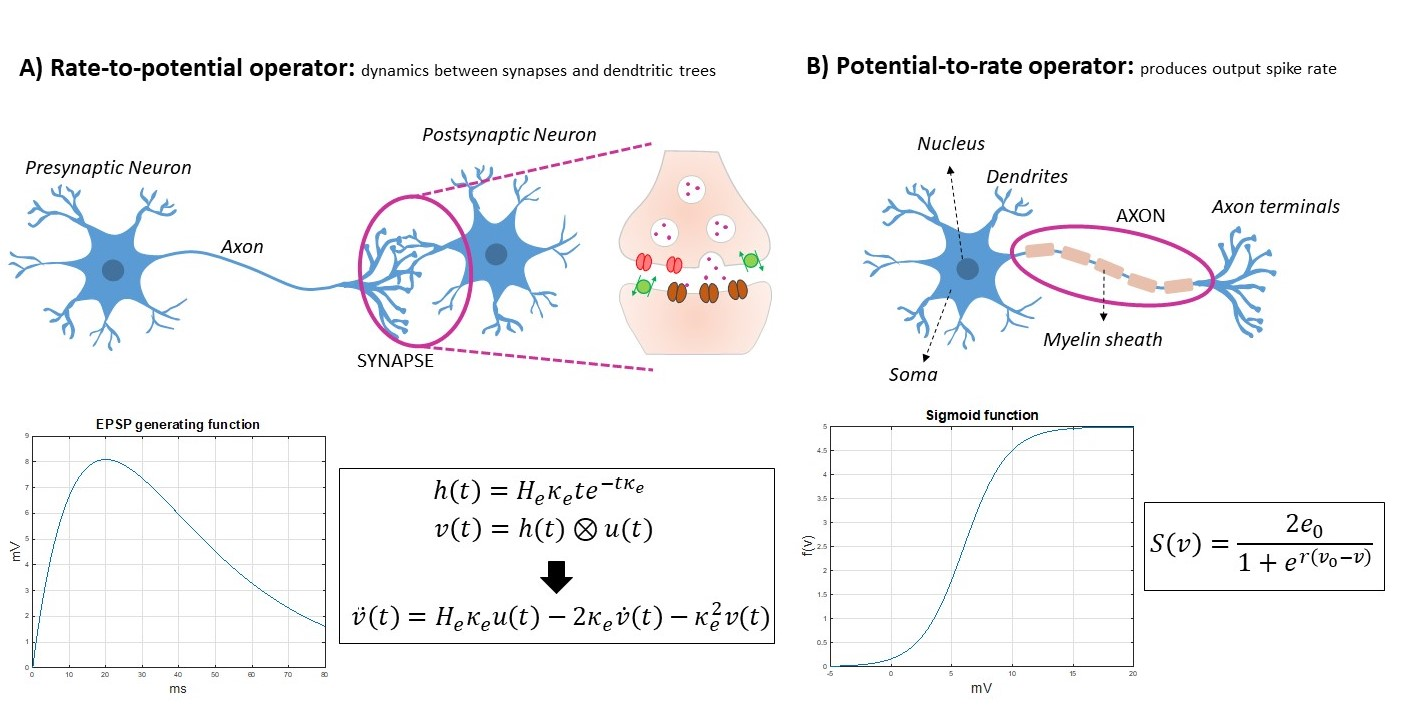
\includegraphics[width=\linewidth]{Images/Common_elem_1.jpg}
    \caption*{\textbf{Figure 4. \textit{Foundational components of NMM to simulate local brain activity.}} Neural populations are composed of \textbf{A)} A rate-to-potential operator describing the postsynaptic potential generated by the firing rates of the presynaptic neurons; and \textbf{B)} a potential-to-rate operator, typically expressed as a nonlinear function, to relate the membrane potential of the neurons to their spiking activity. These two operators are the basic components of NMM and shape the dynamics and behavior of the system.}
    \label{fig:Common_NMM}
\end{figure}
%TC:endignore


%\begin{figure}[H] 
 %   \centering
  %  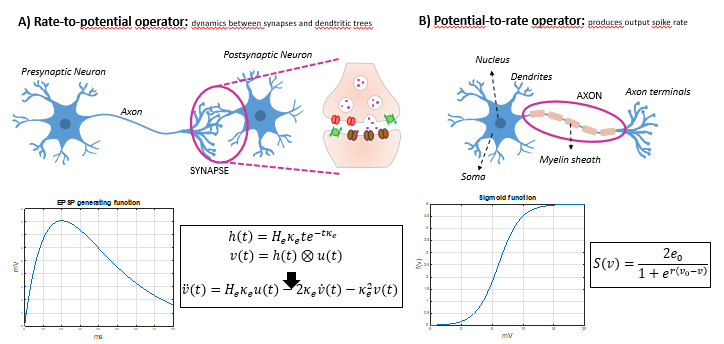
\includegraphics[scale=0.9]{Images/Operators.png}
  %  \caption*{\textbf{Figure 3.  \textit{Common elements in neural mass models.}} Each neural population is defined by a rate-to-potential operator (A) and a potential-to-rate operator (B) }.
   % \label{fig:Common_NMM}
%\end{figure}

%TC:ignore
\section{Methods}


%\subsection{Detailed presentation of alpha rhythm NPMs} 
\subsection{Alpha rhythm models} 
%TC:endignore
With the basic conceptual and mathematical background established, the four selected NPMs representing alternative theories for the genesis of alpha activity - JR, MDF, LW, and RRW - will now be introduced in full detail. In the next few sections we present for each model i) topological and circuit diagrams with the corresponding equations, ii) alpha rhythm simulations using both numerical (differential equation) and analytical (linearized algebraic) expressions\footnote{With regards to nomenclature: originally we aimed to find a generalized mathematical form that covered all four models of interest, and allowed for a single nomenclature with clear correspondences across models indicated by variable and parameter names. After further exploration we determined however that this is not possible without an unhelpfully large amount of abstraction. We have therefore elected to write out the equations following exactly the original and/or primary literature sources.}, and iii) a didactic commentary. By comparing and contrasting these models in the subsequent sections, we aim to provide insights into their activity regimes and dynamical properties. All model parameters are listed in Supplementary S.6 along with their definitions. Selected equations are included in figures, while the complete equations for all models can be also be found in Supplementary S.6 for reference, and the Python code implementations in the GitHub repository accompanying this paper (https://github.com/GriffithsLab/Bastiaens2024\_AlphaModels). 

%TC:ignore
\subsubsection{Jansen-Rit model}
%TC:endignore
Based on Lopes da Silva’s lumped parameter formulation \citep{lopes1974model}, the JR model was one of the first of its kind to reproduce a broad range of EEG oscillation frequencies (including alpha), as well as evoked response waveform, by describing the macroscopic electrophysiological activity within a cortical column \citep{jansen1993neurophysiologically, jansen1995electroencephalogram}. Analogously to \citet{zetterberg1978performance}, JR developed the model with three interconnected neural populations: pyramidal projection neurons ($y_0$), excitatory ($y_1$) and inhibitory ($y_2$) interneurons forming two feedback loops - a (fast) excitatory feedback loop and a slow inhibitory feedback loop (Fig. 5A) \citep{Knösche2015}. The output  $y_1-y_2$ represents the net PSP on the pyramidal cell dendrites, which is defined as the difference between the EPSP from the excitatory population and the IPSP from the inhibitory population. This quantity corresponds to the membrane potential of pyramidal neurons which can also be understood as the output of the columnar microcircuit that is transmitted to other adjacent and distal brain areas. Since pyramidal neurons have their apical dendrites in the superficial layers of the cortex where the postsynaptic potentials are summated, their activity is the primary contribution to the measured EEG signal \citep{jansen1995electroencephalogram, grimbert2006analysis}.  

The mathematical expression of the sigmoid for JR is defined as
\begin{equation}
     S(v)=\frac{2e_0}{1+e^{r(V_0-v)}}
 \end{equation}
 with $e_{0}$ representing the firing rate at threshold (and $2e_{0}$ the maximum firing rate), $r$ denoting the variance of firing thresholds, and $V_{0}$ corresponding to the mean firing threshold. The impulse response is expressed as follows
 \begin{equation}
   h(t)=\alpha \beta te^{-\beta t}    \qquad \text{for t} > 0, 
 \end{equation}
 
 and corresponds to an alpha function. The parameter $\alpha$ is defined as the maximum amplitude of the postsynaptic potential, and $\beta$ represents a sum of the reciprocal of the time constant of the passive membrane and all other spatially distributed delays present in the dendritic network, condensed into a single lumped term. For the excitatory  populations $\alpha$, $\beta$ in Eq. 4 correspond to the terms $A$, $a$ in Fig. 5 respectively, and for the inhibitory population $\alpha$, $\beta$ are $B$, $b$.
 
After transforming the above impulse response in the Laplace domain, we are able to fully define the system with second-order differential equations (derivation provided in Supplementary S.1). The final set of differential equations are detailed in Fig. 5B with the numerically integrated time series output, the associated power spectrum, as well as the power spectrum obtained with the transfer function in Fig. 5C.
It is important to note that the connectivity parameters $C_{1}$ and $C_{3}$ are slightly different than $C_{2}$ and $C_{4}$ based on the mathematical expression. As noted by \citet{cook2021neural}, JR assumes that pyramidal cell population equally synapses onto the other two populations. However, the synaptic coefficients at the dendrites of the excitatory and inhibitory populations differ. The inverse is also observed with the pyramidal cells, as the synaptic coefficient at the dendrites of the pyramidal cells is fixed (1 and -1 for excitatory and inhibitory interneurons respectively), but the synaptic connectivity changes. Therefore, $C_{1}$ and $C_{3}$ represent these former synaptic coefficients and $C_{2}$ and $C_{4}$ are the latter connectivity constants, as seen in the detailed schematic. However, in practice, they all represent connectivity strength and can be likened and associated with each other. Further details are provided in Supplementary S.6 in the details of the JR model equations. 

%TC:ignore
\begin{figure}[H]
    \centering
    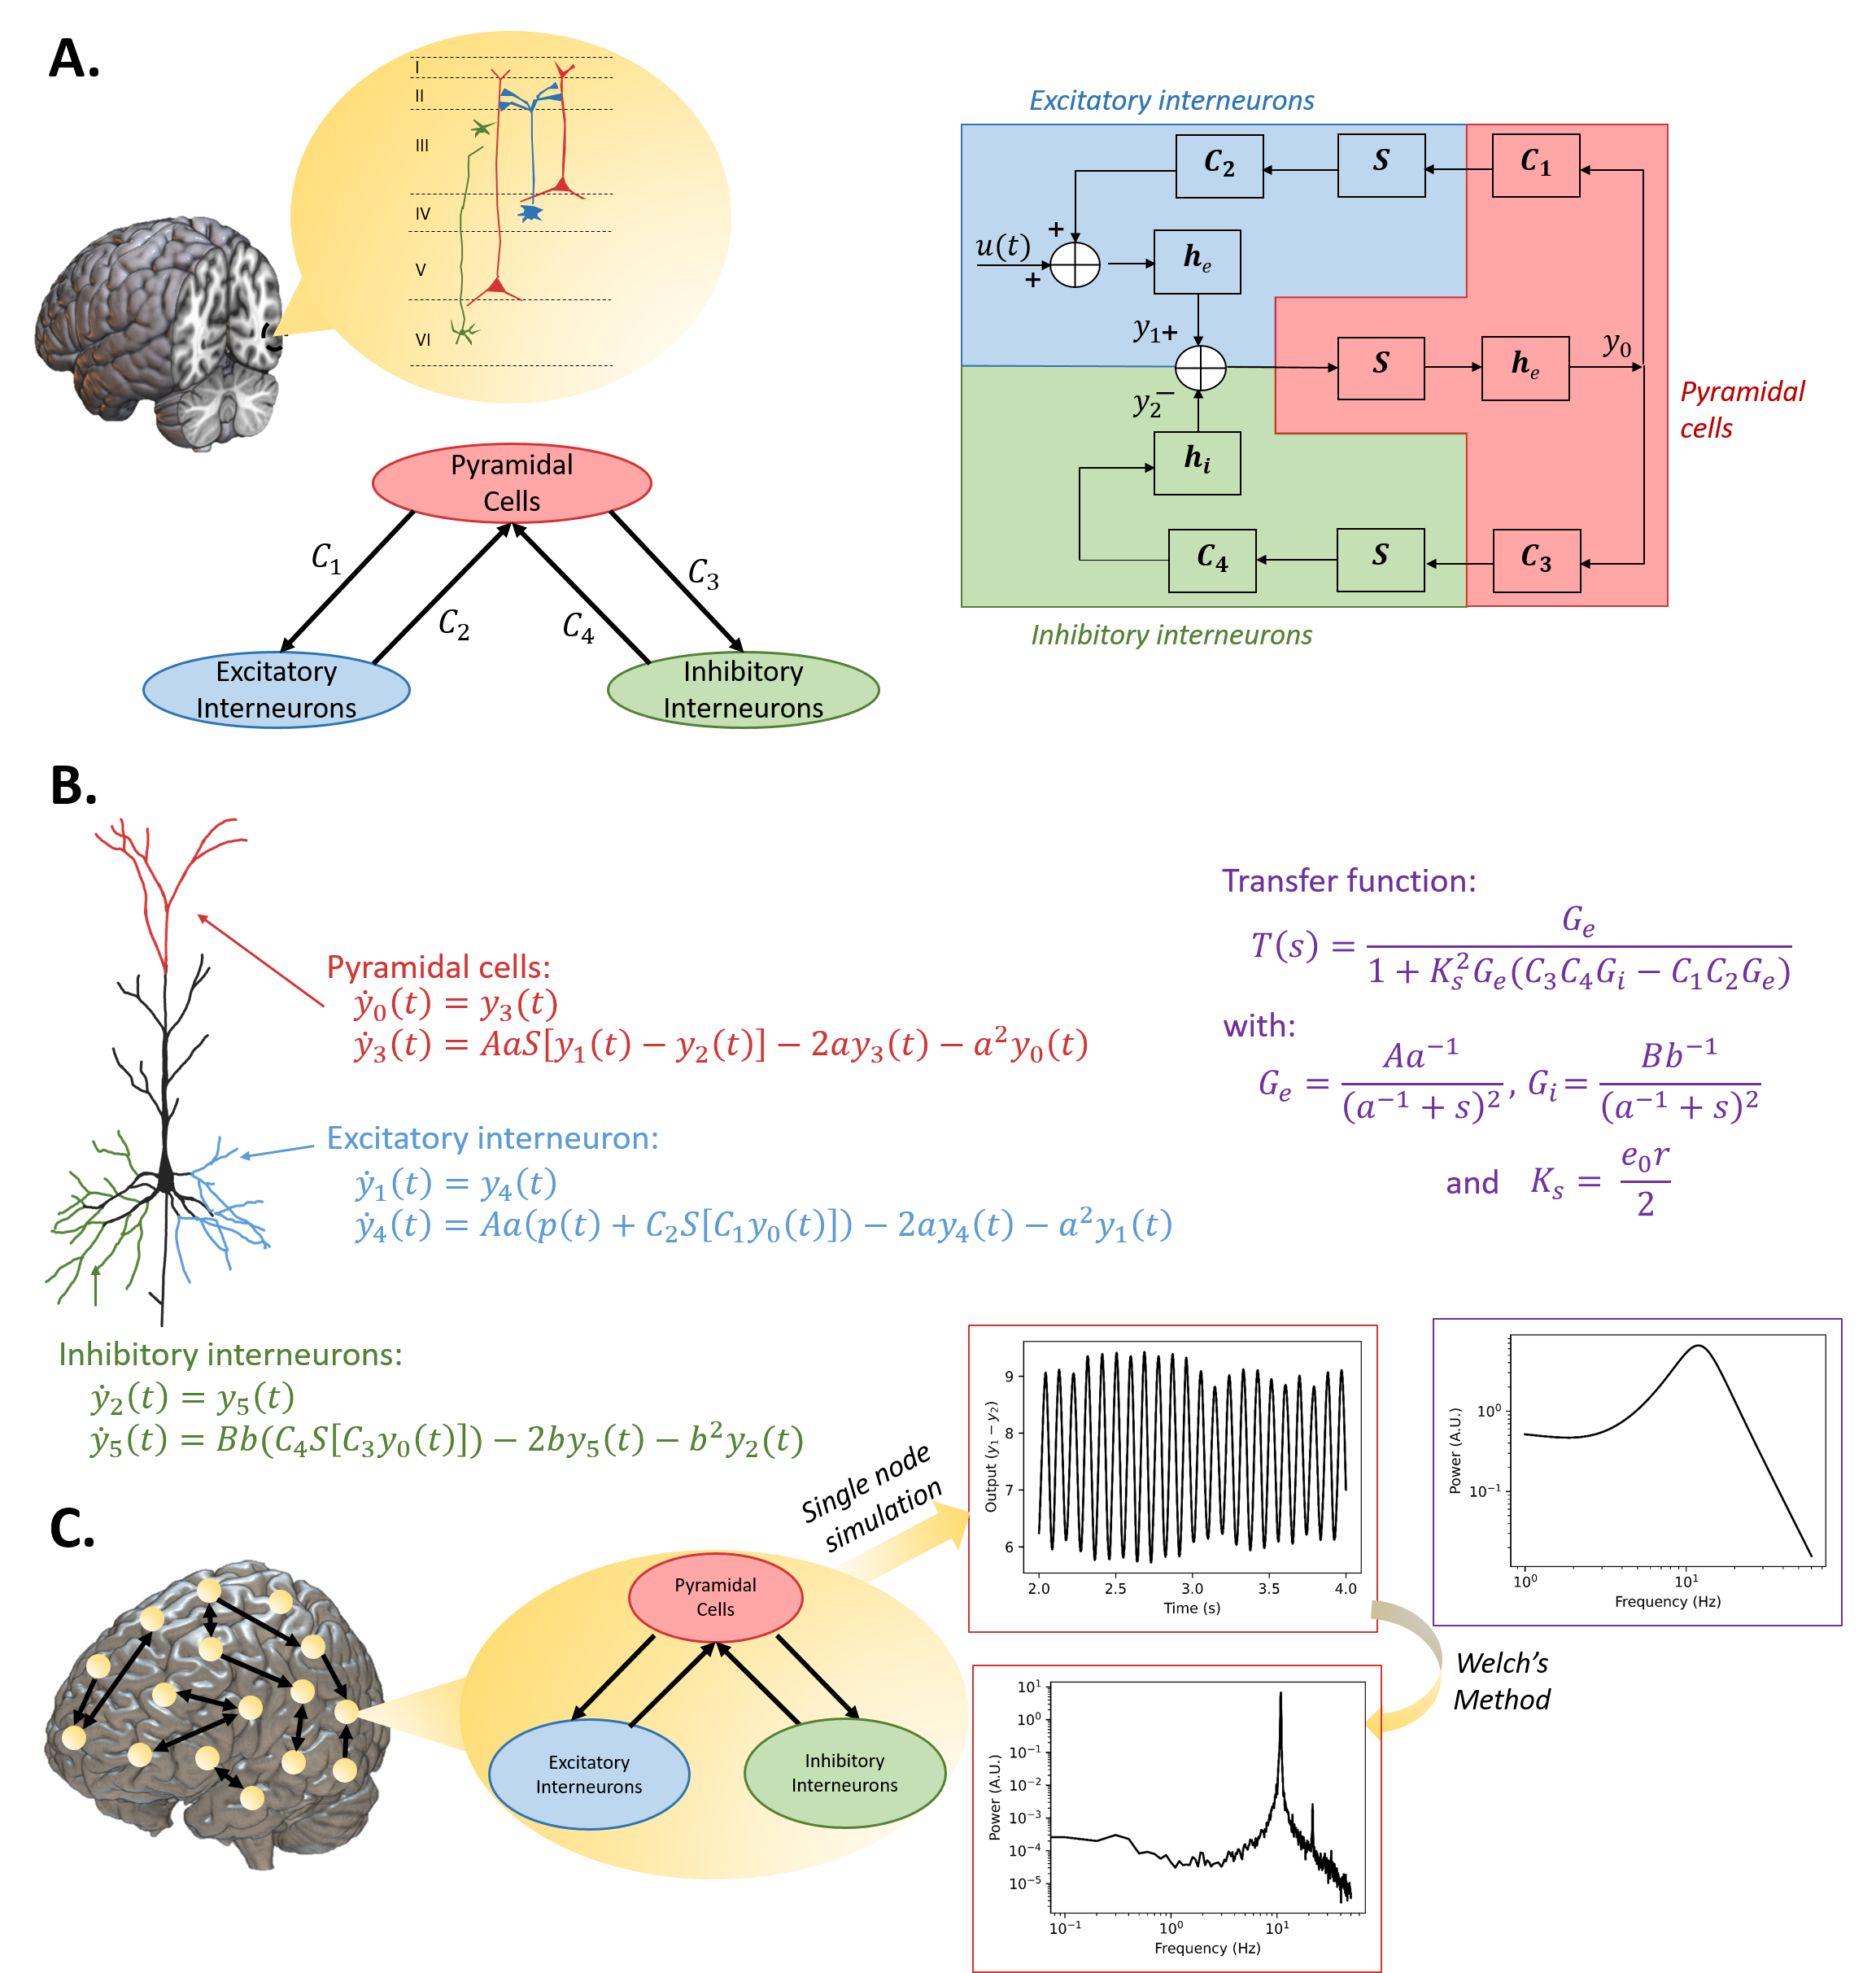
\includegraphics[scale=0.45]{Images/Jansen_rit_schematic_4.png}
    %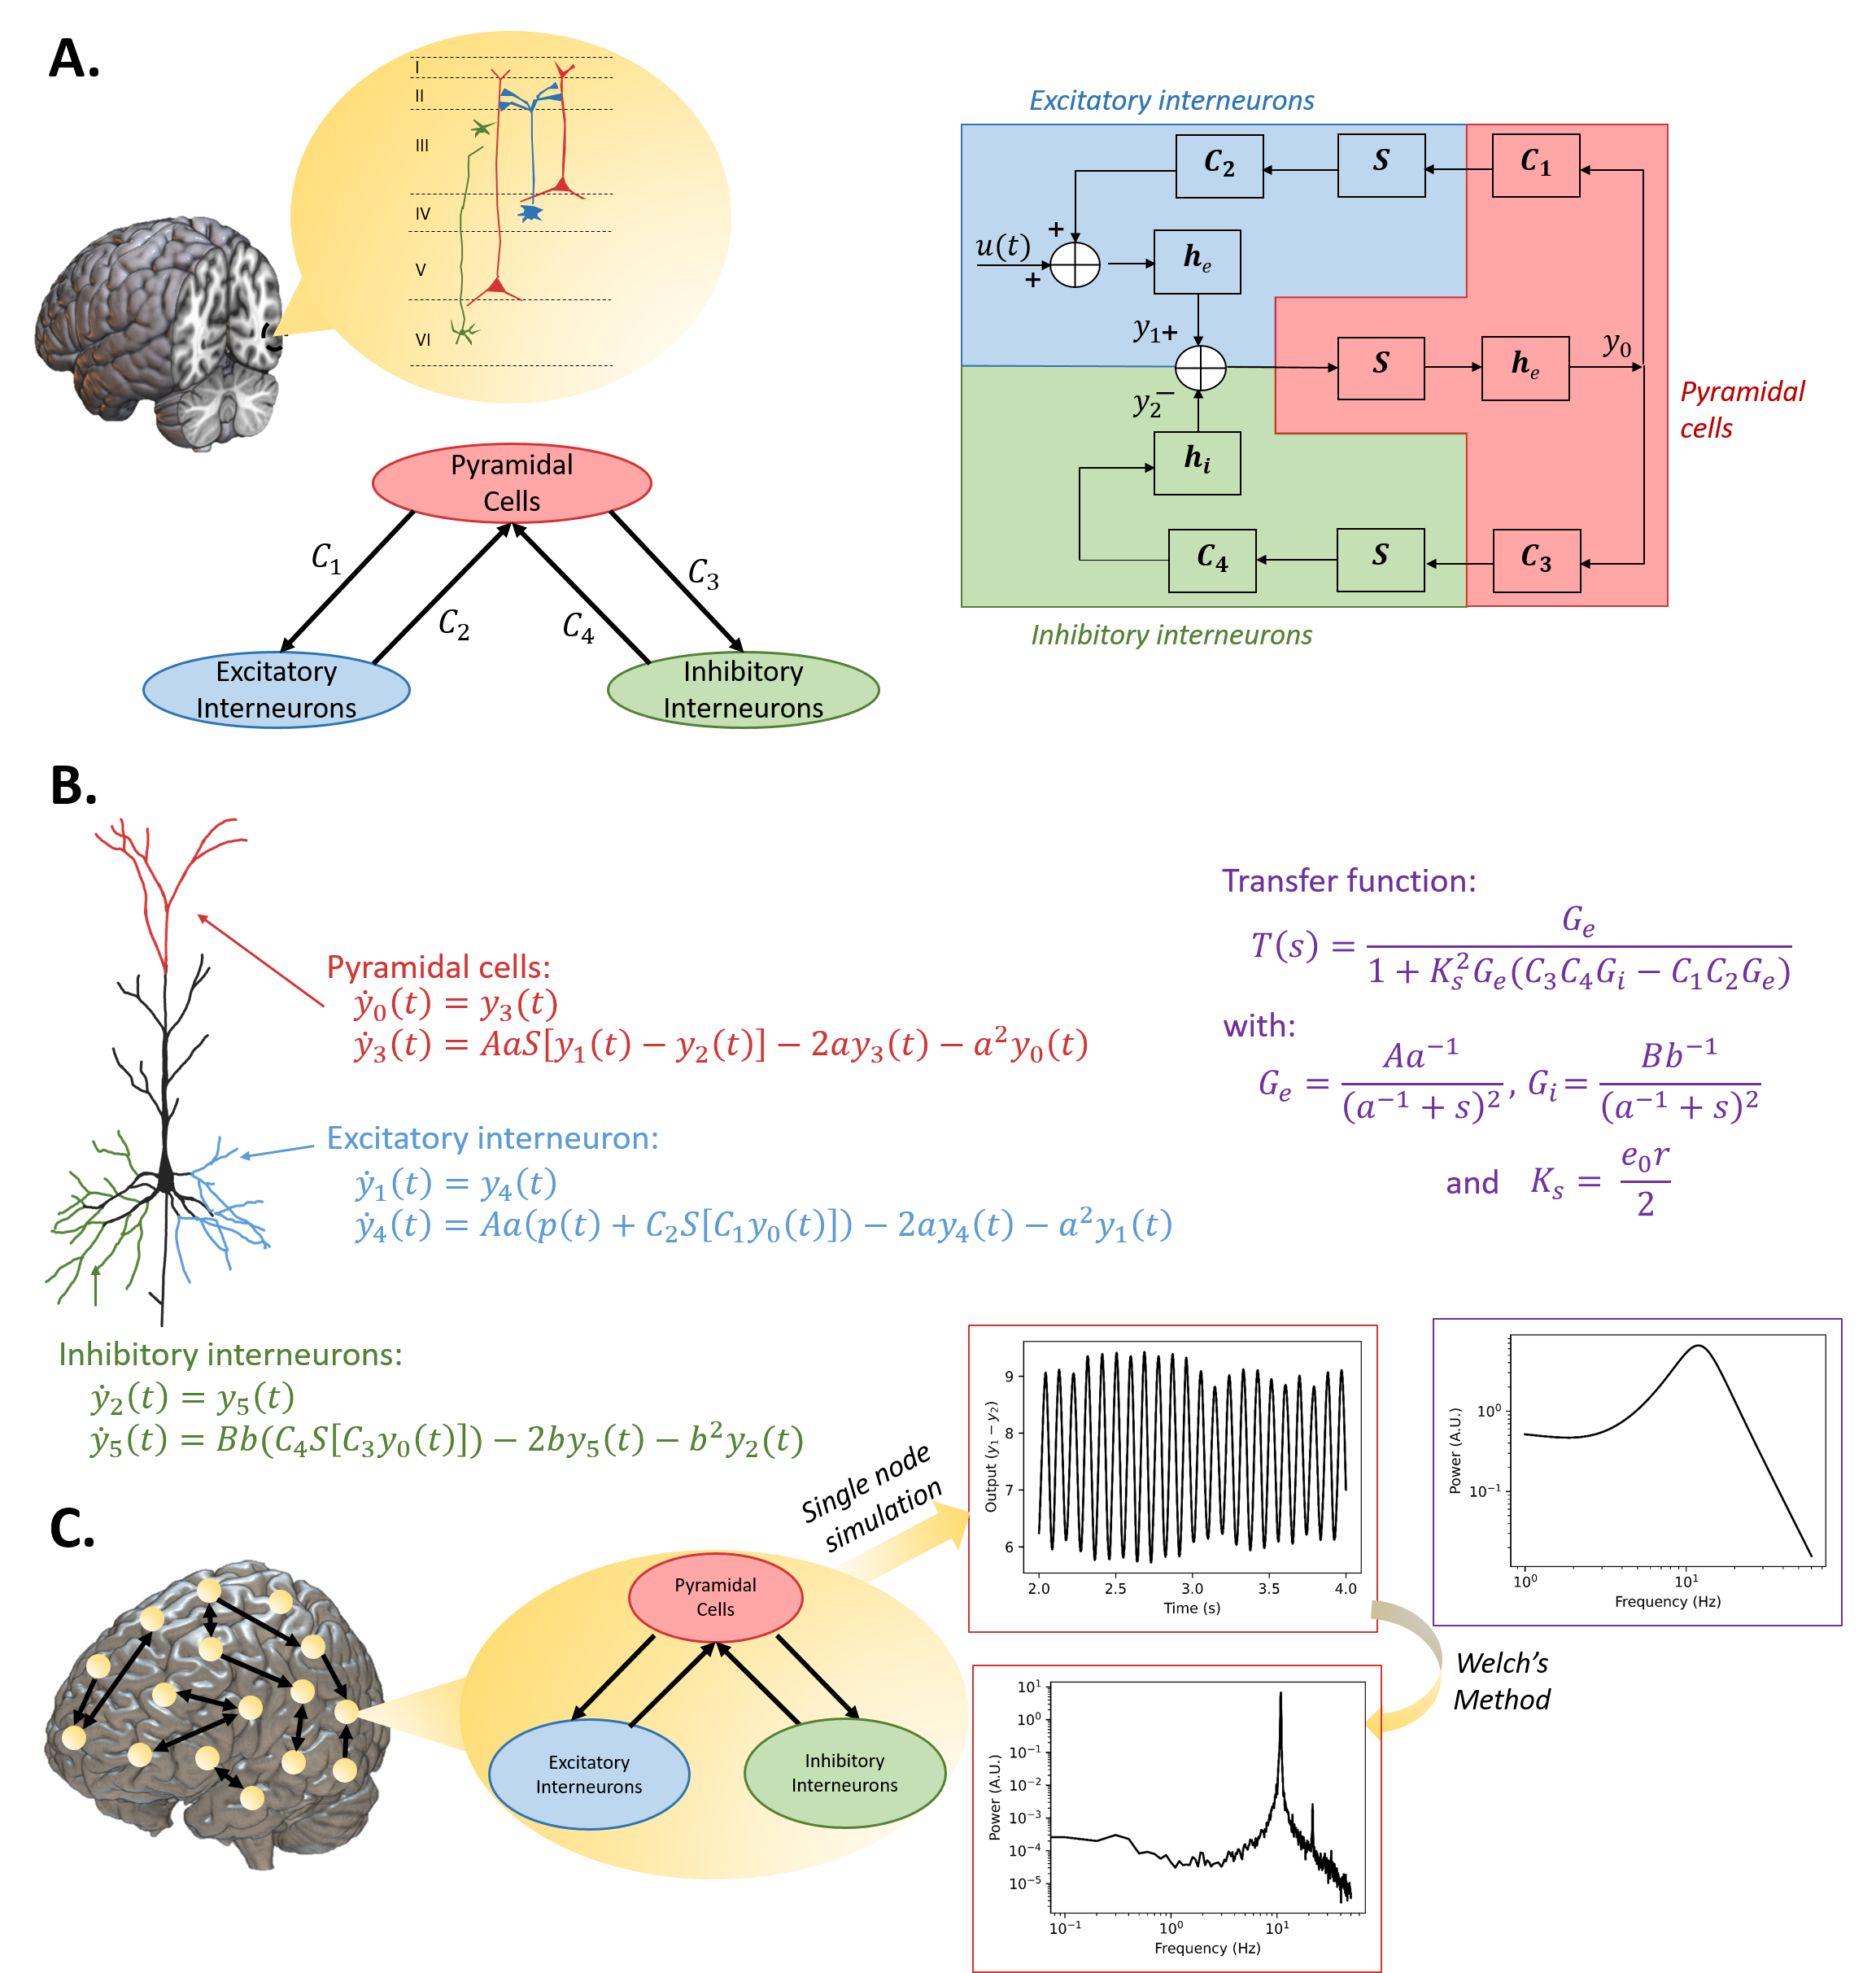
\includegraphics[scale=0.5]{Images/Jansen_rit_schematic_4.png}
    \caption*{\textbf{Figure 5.  \textit{JR model topography, schematic, numerical and analytical mathematical expression, and alpha simulation results}}. \textbf{A)} General structure of the model, along with a detailed schematic that includes the operators and representations of the connectivities; \textbf{B)} Left: Numerical mathematical expression for each neural population; Right: Transfer function of the model derived using control graph analysis; \textbf{C)} Simulation outputs of the model with standard parameters (time series, power spectrum estimated from the time series and analytical power spectrum)}
    \label{fig:JR_full}
\end{figure}
%TC:endignore
 % \begin{minipage}{\textwidth}
  %\begin{minipage}[b]{0.49\textwidth}
  %\fontsize{8}{11}\selectfont 
   % \hspace{-0.9cm}  
    %\begin{tabular}{|c|p{7cm}|p{1.5cm}| }
    %\hline
    %Symbol & \multicolumn{1}{|c|}{Description} & \multicolumn{1}{|c|}{Value}  \\ 
    % \hline
    %{$e_{0}$} & Maximum firing rate of a neural population & 2.5 s$^{-1}$ \\ 
    % \hline
   %  $V_{0}$ & Firing threshold	& 6 mV \\ 
   %  \hline
   %  r	& Slope reflecting the variance of firing thresholds within the population &	0.56 mV$^{-1}$ \\
   %  \hline
    % A &	Maximum amplitude of excitatory PSP (EPSP)&	3.25 mV \\
    % \hline
    % B & Maximum amplitude of inhibitory PSP (IPSP) &	22 mV \\
   %  \hline
    % a and b &	Lumped representation of the sum of the reciprocal of the time constant of passive membrane and all other spatially distributed delays in the dendritic network	& a = 100 s$^{-1}$ \newline b = 50 $s^{-1}$\\
   % \hline
   % $C_{1}$ & Connectivity constant: Represents the number of synapses made by the feed forward neurons to the dendrites of the excitatory feedback loop &	$C_{1}=C=135$\\
   % \hline
   % $C_{2}$ & Connectivity constant: Proportional to the number of synapses made by the excitatory feedback loop to the dendrites of the feedforward neurons & $C_{2}=0.8C$\\
   % \hline
   % $C_{3}$ & Connectivity constant: number of synapses made by the feedforward neurons to the dendrites of the inhibitory feedback loop & $C_{3}=0.25C$\\
   % \hline
   % $C_{4}$	& Connectivity constant: Proportional to the number of synapses made by the inhibitory feedback loop to the dendrites of the feedforward neurons & $C_{4}=0.25C$\\
  %  \hline
   % P(t) & External pulse density consisting of activity originating from adjacent and more distant cortical columns and from subcortical structures (e.g. thalamus) & Uniform noise (120-320)\\
   % \hline
   % \end{tabular}
    %  \captionof{table}{A table beside a figure}
   % \end{minipage}
   %   \begin{minipage}[b]{0.6\textwidth}
   % \centering
   % 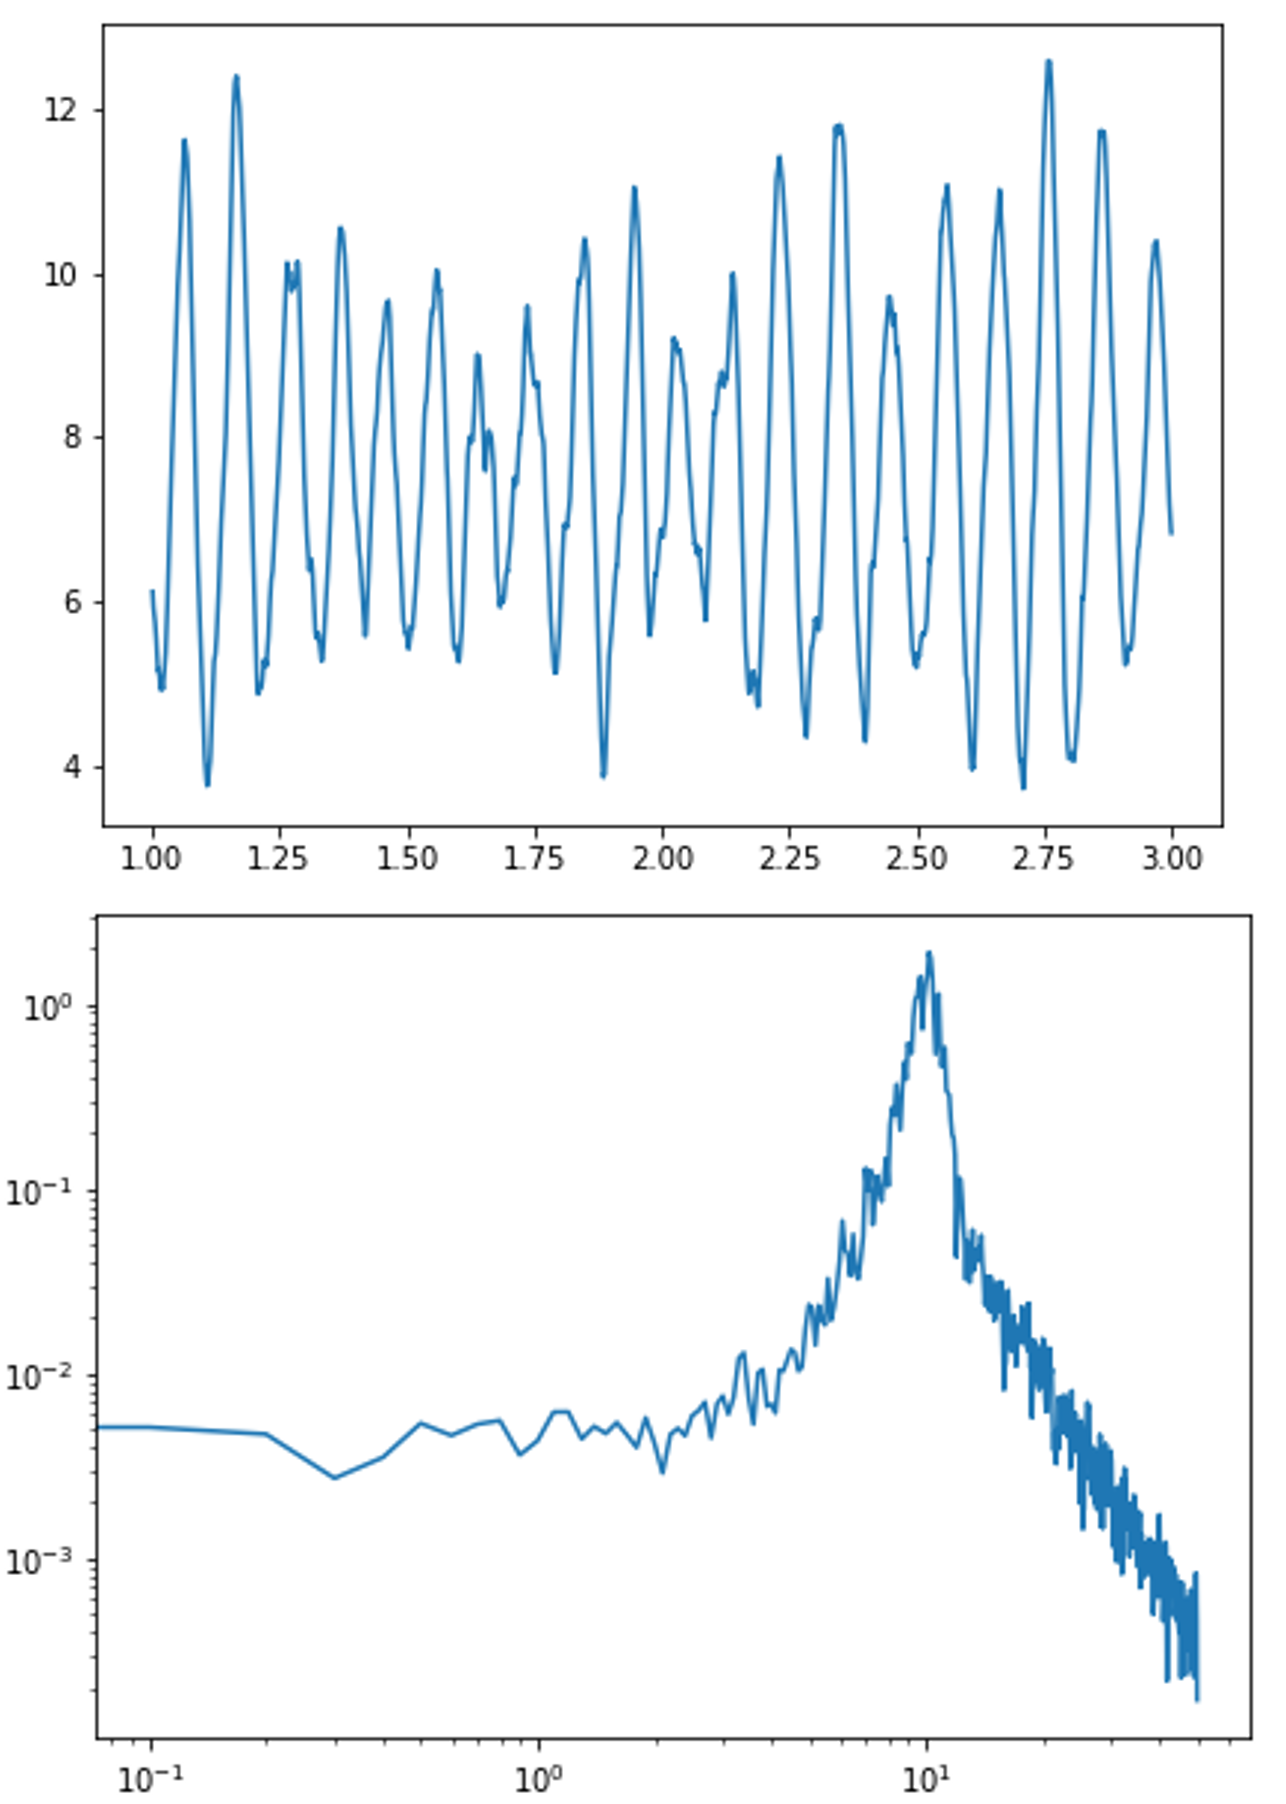
\includegraphics[scale=0.3]{Images/JR_oscillations.png}
  %  \captionof{figure}{A table beside a figure}
 % \end{minipage}
 % \hfill
 % \end{minipage}
%
% Pyramidal cells
% \begin{align}
%     \dot{y_0}(t) &= y_3(t) \\ \notag
%     \dot{y_3}(t) &= AaSigm[y_1 (t)-y_2 (t)]-2ay_3 (t)-a^2 y_0 (t)
% \end{align}
%
% Excitatory interneurons
% \begin{align}
%     \dot{y_1} (t) &= y_4 (t) \\ \notag
%     \dot{y_4} (t) &= Aa(p(t)+C_2 Sigm[C_1 y_0 (t)])-2ay_4 (t)-a^2 y_1 (t)
% \end{align}
%
% Inhibitory interneurons
% \begin{align}
%     \dot{y_2} (t) &= y_5 (t) \\ \notag
%     \dot{y_5} (t) &= Bb(C_4 Sigm[C_3 y_0 (t)])-2by_5 (t)-b^2 y_2 (t)
% \end{align}
%
% Analytical:\\
%
% \begin{equation}
%         Y(s) = \frac{PG_e}{1+K_s^2 G_e (C_3 C_4 G_i-C_1 C_2 G_e)}
% \end{equation}
% Where 
% P is the input to the transfer function (constant for example)
% \begin{align}
%     G_e &= \frac{Aa}{(a+s)^2} \\
%     G_i &= \frac{Bb}{(b+s)^2} 
% \end{align}
% (Transfer function of impulse response)
% \begin{equation}
%     K_s=\frac{e_0 r}{2}
% \end{equation}
% (Linear approx. of sigmoid function around equilibrium point)

%TC:ignore
\subsubsection{Moran-David-Friston model}
%TC:endignore
% Chose this extension because JR is not capable of reproducing higher fr phenomena problematic to replicate neuropathology 
Many models inspired by JR emerged in the years following their introduction. One of the most influential of these was proposed by \citet{david2003neural}, later extended by \citep{moran2007neural}. The MDF model and the JR model (of which it is an indirect extension) thus share many similar features, and are interesting to compare in terms of the new elements included in \citet{david2003neural} and \citep{moran2007neural}. One such element is the addition of recurrent inhibitory connections, which were introduced by \citep{moran2007neural} in order to enable the generation of a wider range of oscillatory frequencies. Another is that the contribution from excitatory and inhibitory populations are separated in the equations, giving rise to independent EPSP and IPSP terms. The quantity used in observation models such as EEG as a measured response corresponds to the difference between these two postsynaptic potentials, resulting in supplementary sets of differential equations. A third main modifications from JR in MDF is the expression of the sigmoid, given by  
\begin{equation}
    S(v)= \frac{1}{1+e^{-\rho_1 (v-\rho_2)}}- \frac{1}{1+e^{\rho_1 \rho_2 }} .
\end{equation}
This differs from the other models surveyed in this paper (cf. Eqs 3, 8, 11) in providing a greater flexibility in its gain behavior, parameterized by  shape and position $\rho_1$ and $\rho_2$. 

The impulse response in MDF is identical to the JR model, and the parameters have the same definition (Supplementary S.6) with some small variable name changes ($\alpha$,$\beta$ = $H_e$,$\kappa_e$ for the excitatory populations, and $\alpha$,$\beta$ = $H_i$,$\kappa_i$ for the inhibitory population).

The paper by \citet{moran2007neural} includes a linearized version of the MDF model that is used to investigate the steady-state responses. For consistency with our analyses of the JR model, here, we have determined an alternative expression for the transfer function (Fig. 6B) using graphical stability analysis.
%TC:ignore
\begin{figure}[H]
    \centering
    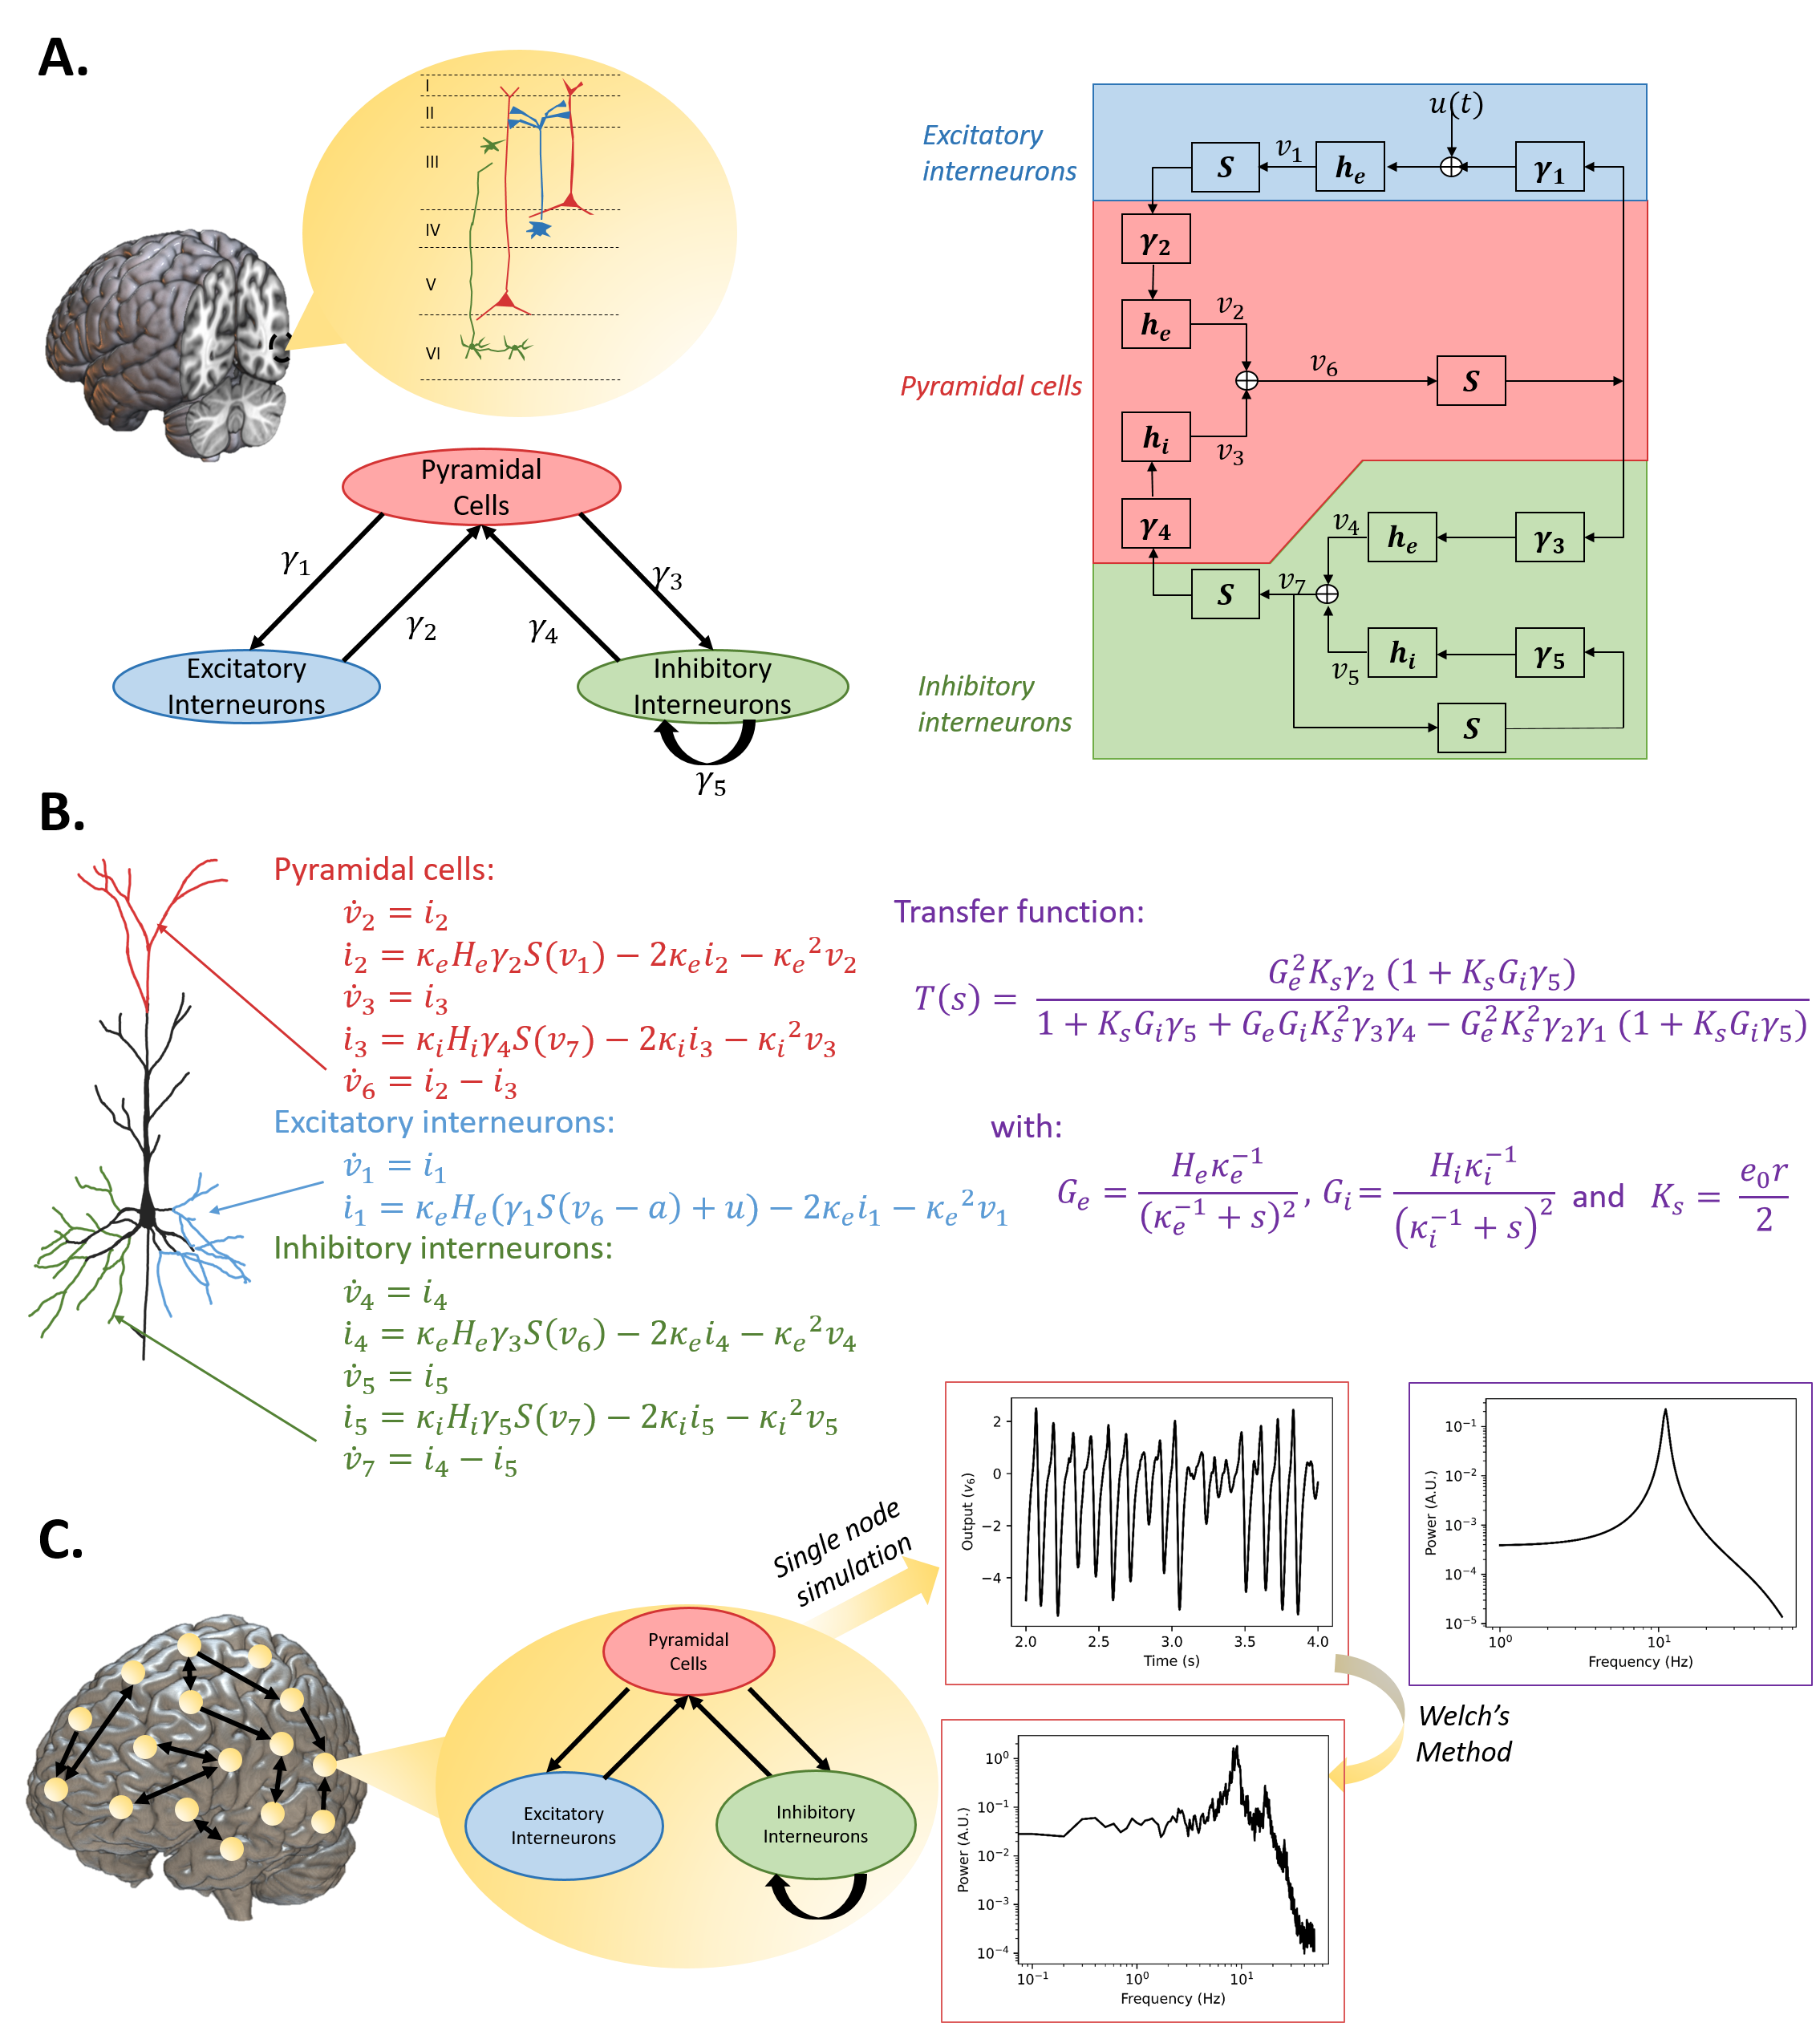
\includegraphics[scale=0.45]{Images/Moran_schematic_4.png}
    %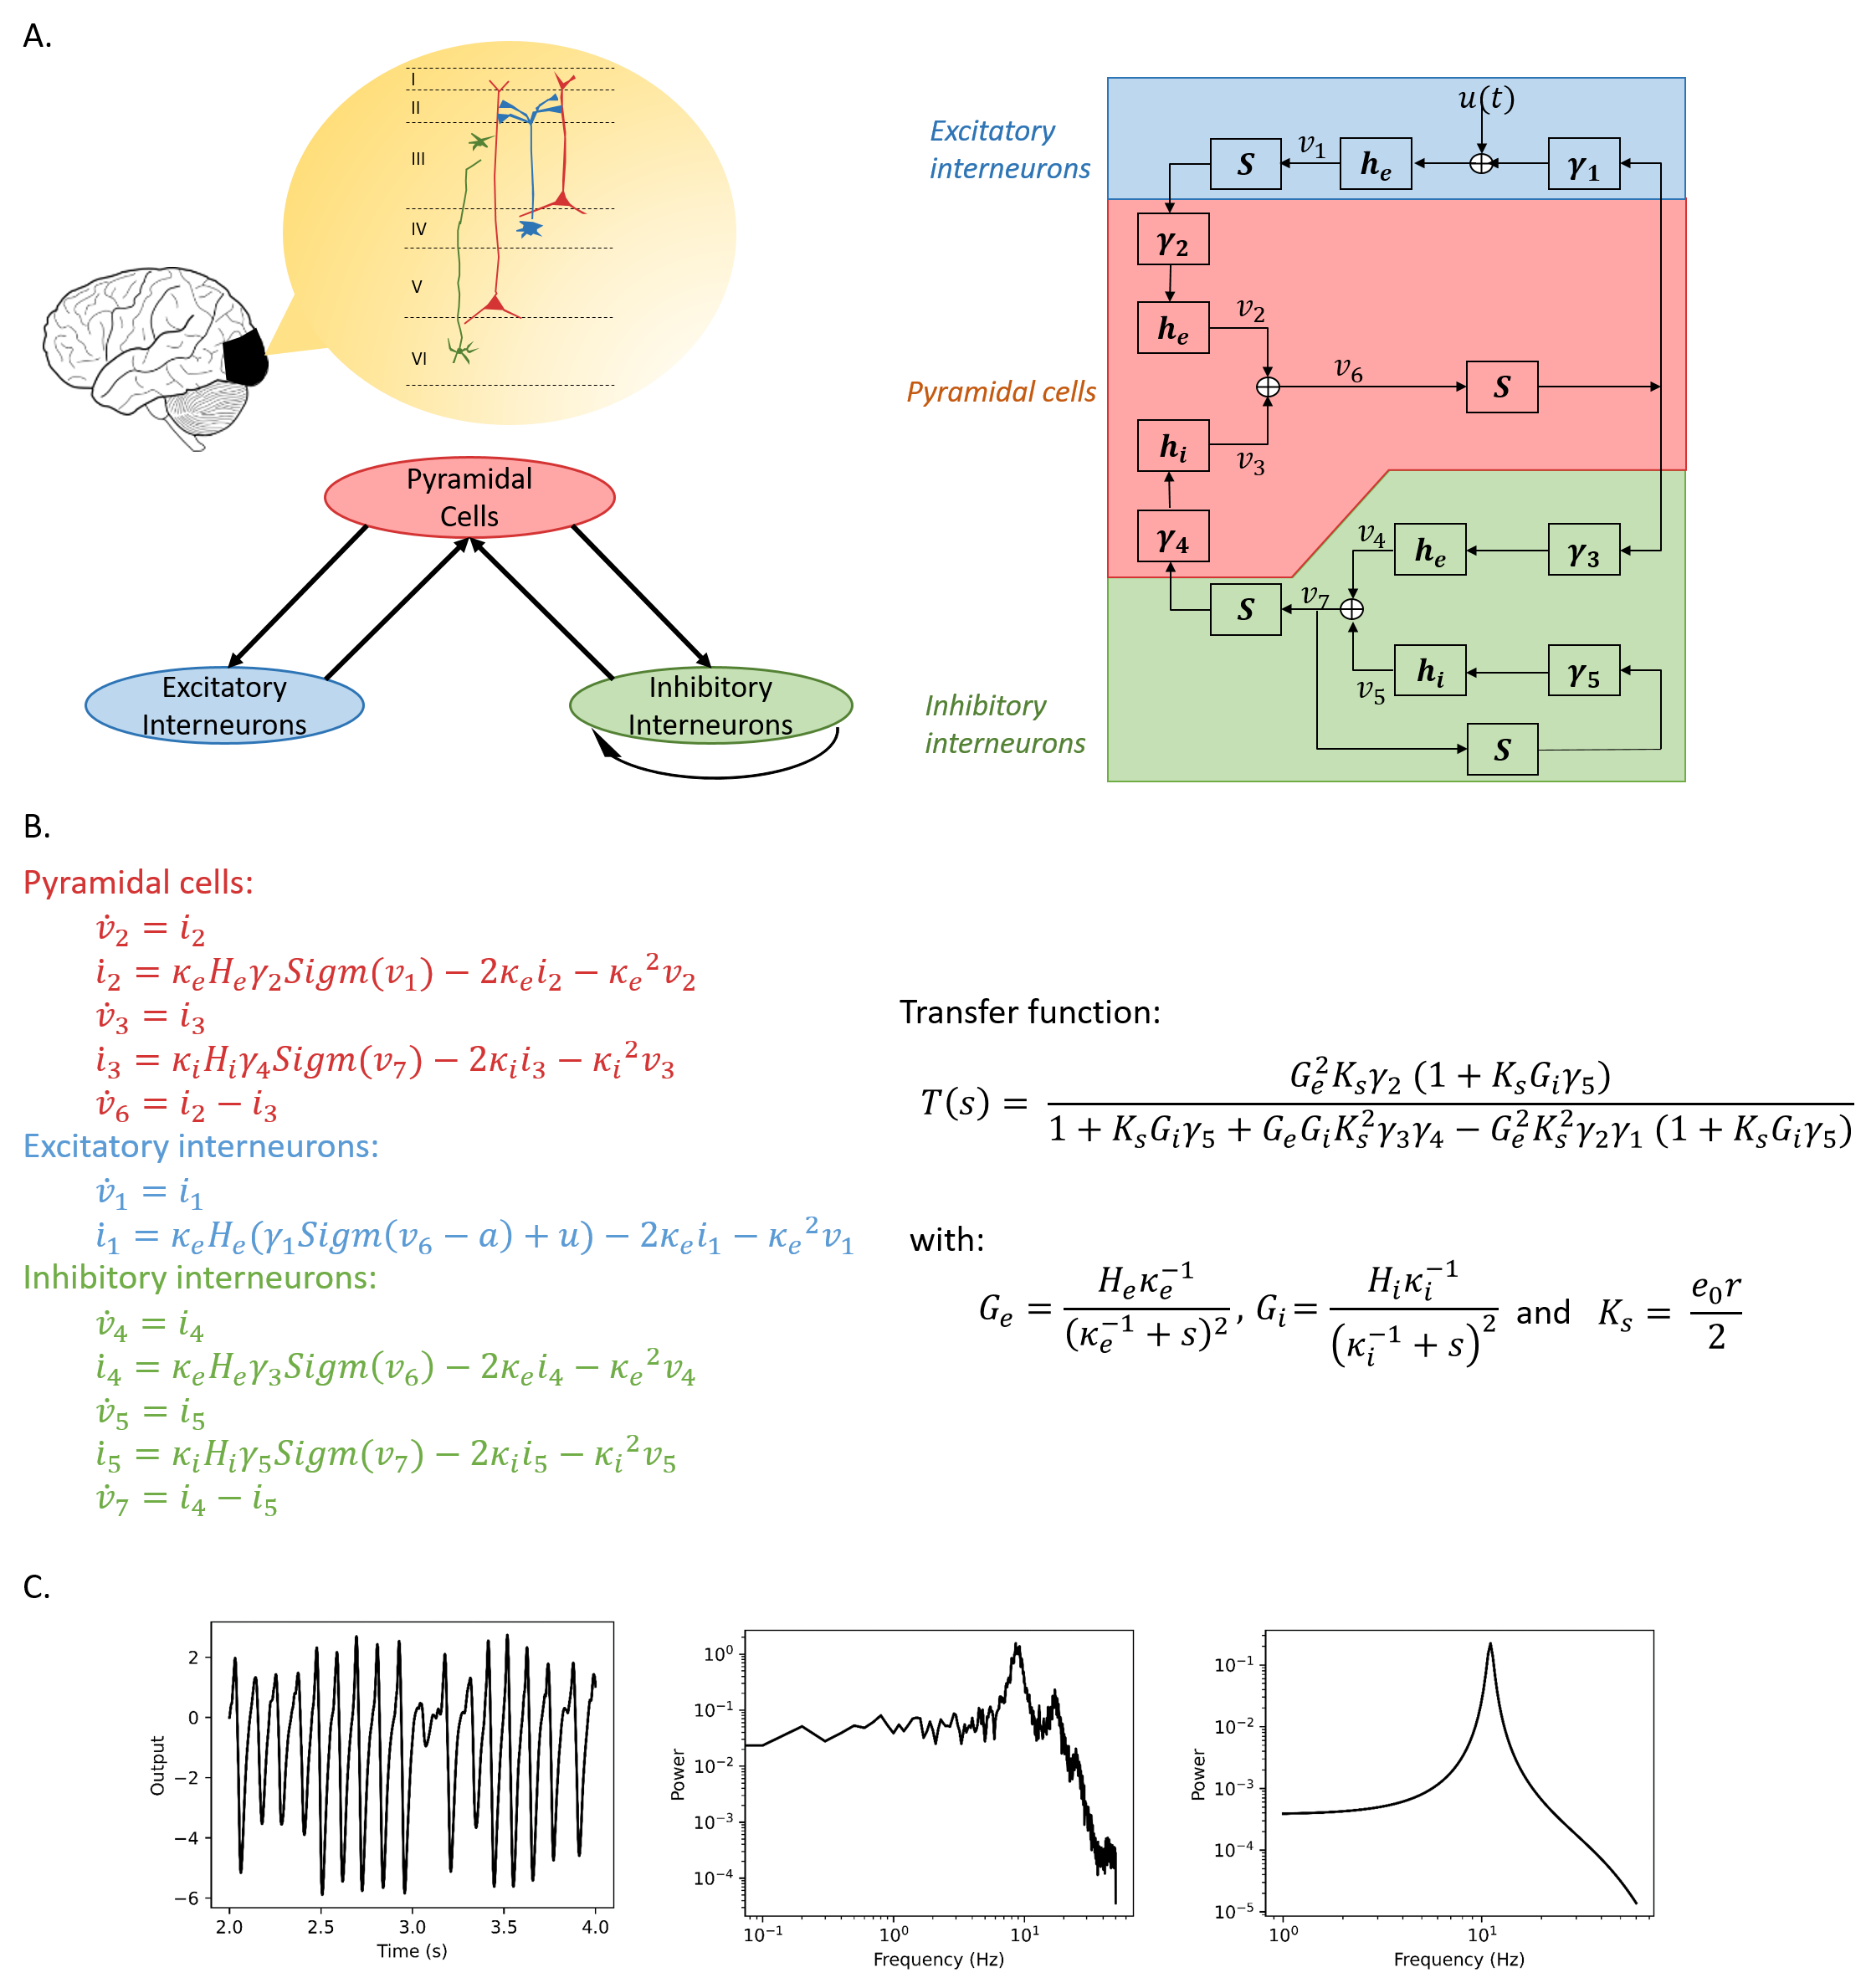
\includegraphics[scale=0.5]{Images/Moran_schematic_2.png}
    \caption*{\textbf{Figure 6.  \textit{MDF model topography, schematic, numerical and analytical mathematical expression and alpha simulation results}} \textbf{A)} Composed of three neural populations with similar wiring structure to JR with the addition of an inhibitory self-connection; \textbf{B)} Left: Numerical mathematical expression for each neural population; Right: Transfer function of the model derived using control graph analysis; \textbf{C)} Simulation outputs of the model with modified parameters to generate alpha oscillations (time series, power spectrum estimated from the time series and analytical power spectrum)}    
    \label{fig:Mor_topography}
\end{figure}
%TC:endignore
%\begin{figure}[H]
%    \hspace{-0.75cm}
 %   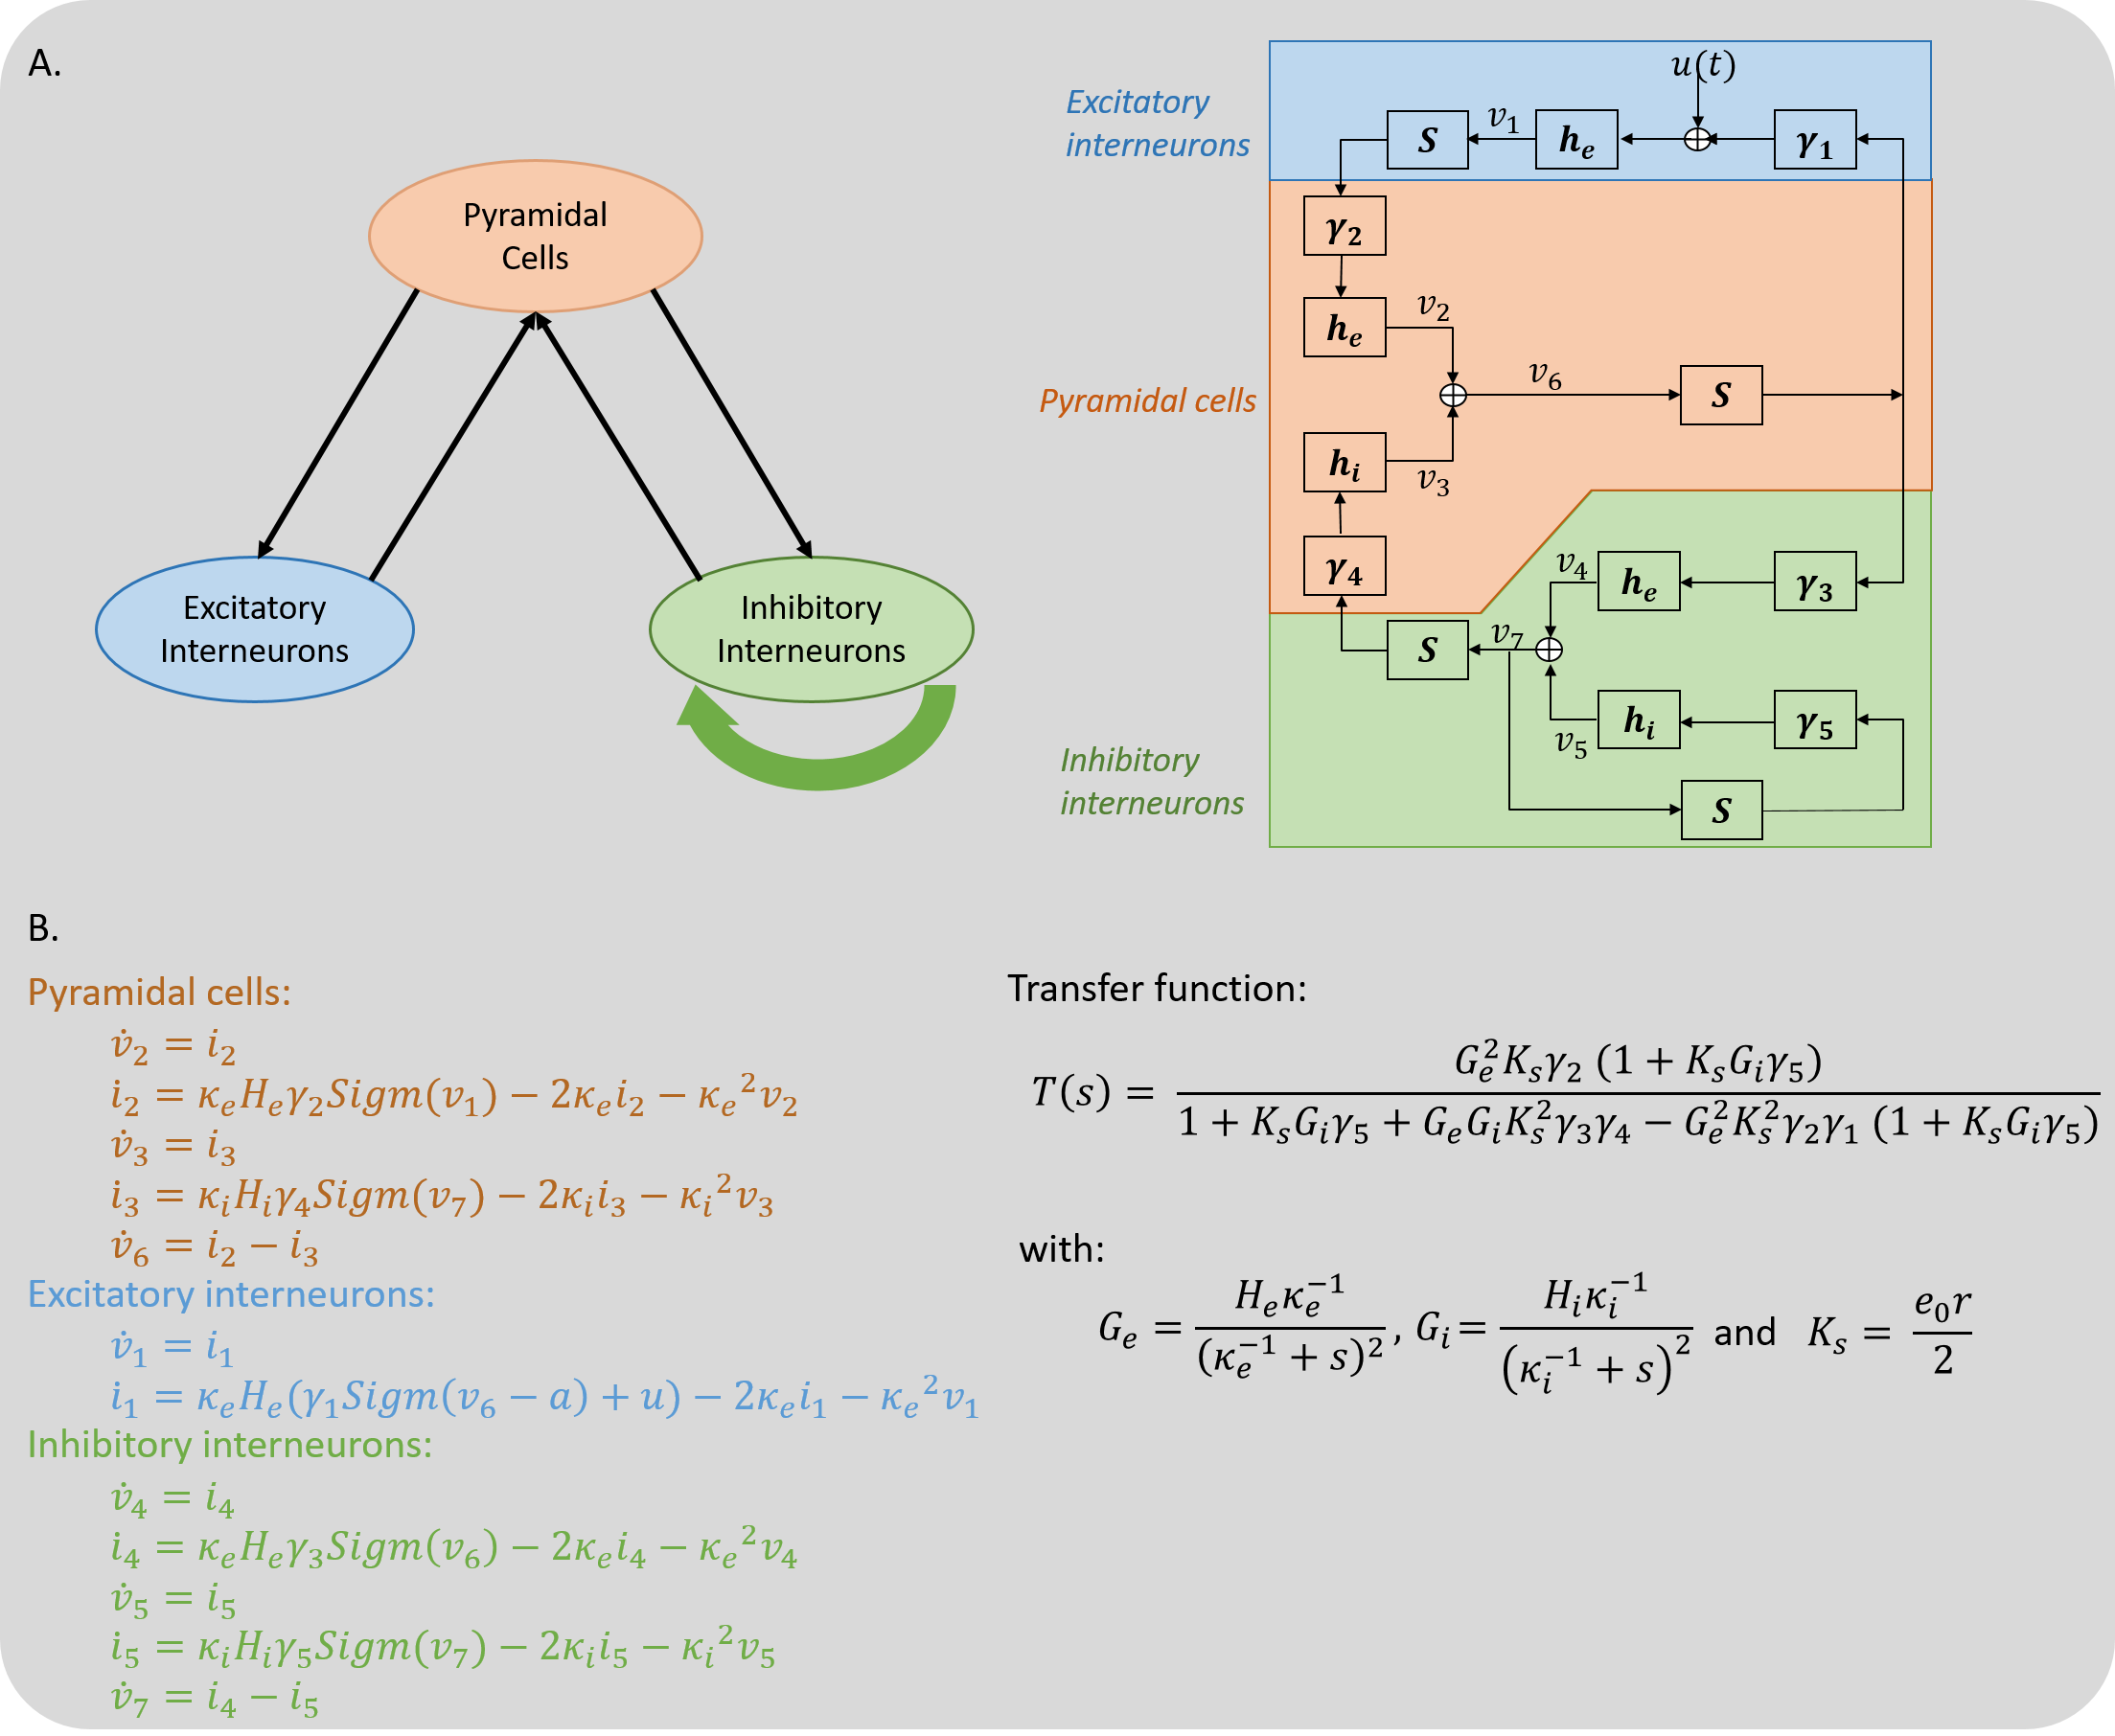
\includegraphics[scale=0.5]{Images/MR_neural_pop_summary.png}
  %  \caption*{\textbf{Figure 6.  \textit{MDF model topography and detailed schematic of interactions between three neural population.}} Composed of three neural population with similar wiring to JR with the addition of the inhibitory self-connection}    
   % \label{fig:Mor_topography}
%\end{figure}


%TC:ignore
\subsubsection{Liley-Wright model}
%TC:endignore
% From Cook: From Eq.(4.38), we can see that because conductance-based synapses are linear in both ua and Va,b, they are bilinear, which introduces another nonlinearity into the equations.

Liley, Wright, and colleagues \citep{liley2001spatially} developed a physiologically parametrizable, two population firing-rate based model of EEG/ECoG dynamics, which differs from JR and MDF in several respects. Most notably, this includes i) inclusion of high-order excitatory and inhibitory neurotransmitter kinetics, ii) presence of synaptic reversal potentials, and iii) the separation of each neural population into both a dendritic and a somatic compartment, yielding two membrane potential state variables per population instead of one. The LW model can be thought of as a convolution-based model with conductance-based synaptic dynamics (where a neuron is regarded as an electrical circuit and the membrane response follows the inflow and outflow of current through ionic channels). These additional features make it more physiologically realistic than e.g. JR, MDF, and WC, albeit at the expense of greater levels of complexity and nonlinearity \citep{cook2021neural}. As with the RRW model discussed below, the LW model was initially formulated as a macroscopic neural field model, with both spatial and temporal variation in the excitatory and inhibitory neural population equations. The version presented here is simplified, however, by neglecting spatial components (setting partial derivatives in the spatial terms of the original equations), and only considering the temporal dynamics - which nevertheless preserves the essential qualitative behavior (alpha-frequency fluctuations) that is our focus in the present paper. These expressions are based on the presentations by \citet{song2019novel} and \citet{hartoyo2019parameter}, in which the LW model was used to explore periodic discharges in acute hepatic encephalopathy and eyes-open/closed alpha-blocking, respectively. 

The sigmoidal firing rate function in the LW model is defined as

\begin{equation}
   S(t)=\frac{S_{(e,i)}^{max}}{1+e^{-(\sqrt{2} V(t)-\mu_{e,i} )/\sigma_{e,i}}}
\end{equation}

where $S_{(e,i)}^{max}$ corresponds to the maximal attainable firing rate, $\mu_{e,i}$ is the spike threshold, and $\sigma_{e,i}$ is the standard deviation for spike threshold. The soma membrane potential is given by 

\begin{equation}
    \tau \dot{V}(t)=V^r-V(t)+\sum \psi(V(t))I(t)
\end{equation}

where $\psi(V(t))=\frac{[V^{eq}-V(t)]}{|V^{eq}-V^r|} $, with $V_{r}$ as the mean resting membrane potential, and $V_{eq}$ the mean equilibrium potential. Similarly to MDF and JR, the impulse response in LW is expressed with an alpha function,

\begin{equation}
    h(t)=\Gamma \gamma te^{1-\gamma t}  \qquad  \text{for t} >  0
\end{equation}

with a postsynaptic potential peak amplitude $\Gamma_{e,i}$ and rate constant $\gamma_{e,i}$.

%TC:ignore
\begin{figure}[H]
    \centering
    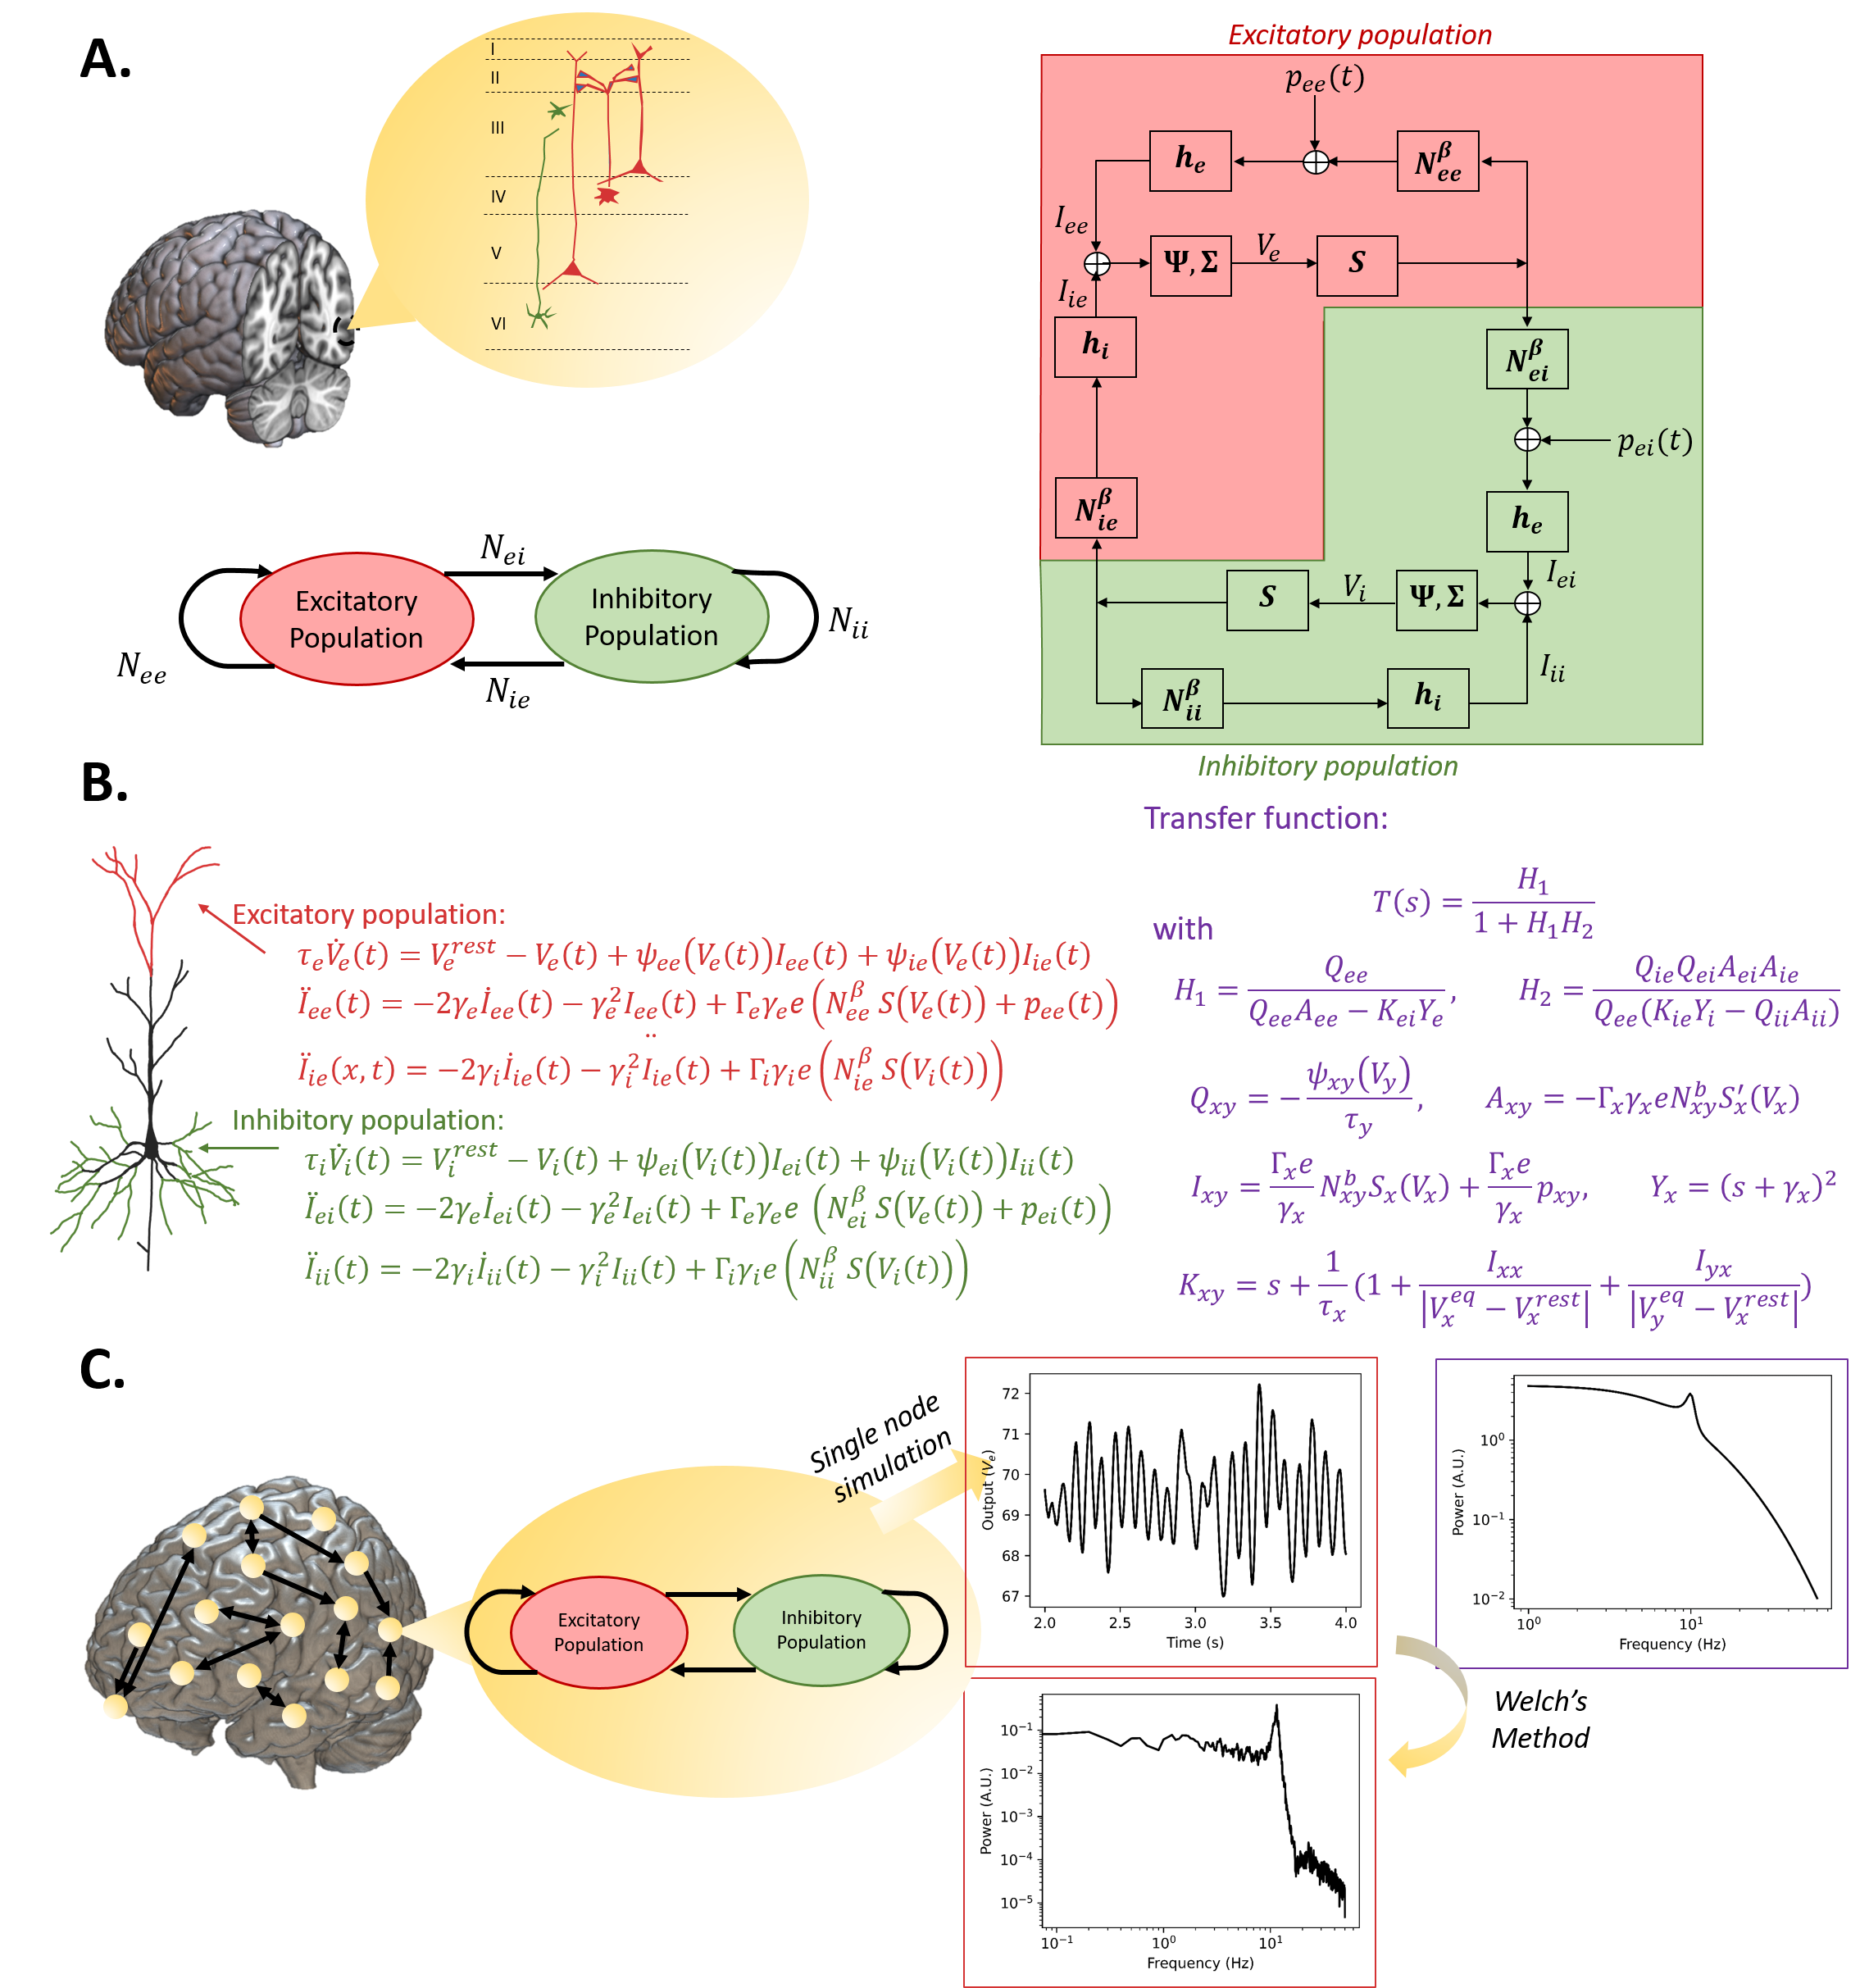
\includegraphics[scale=0.45]{Images/Liley_schematic_3.png}
    %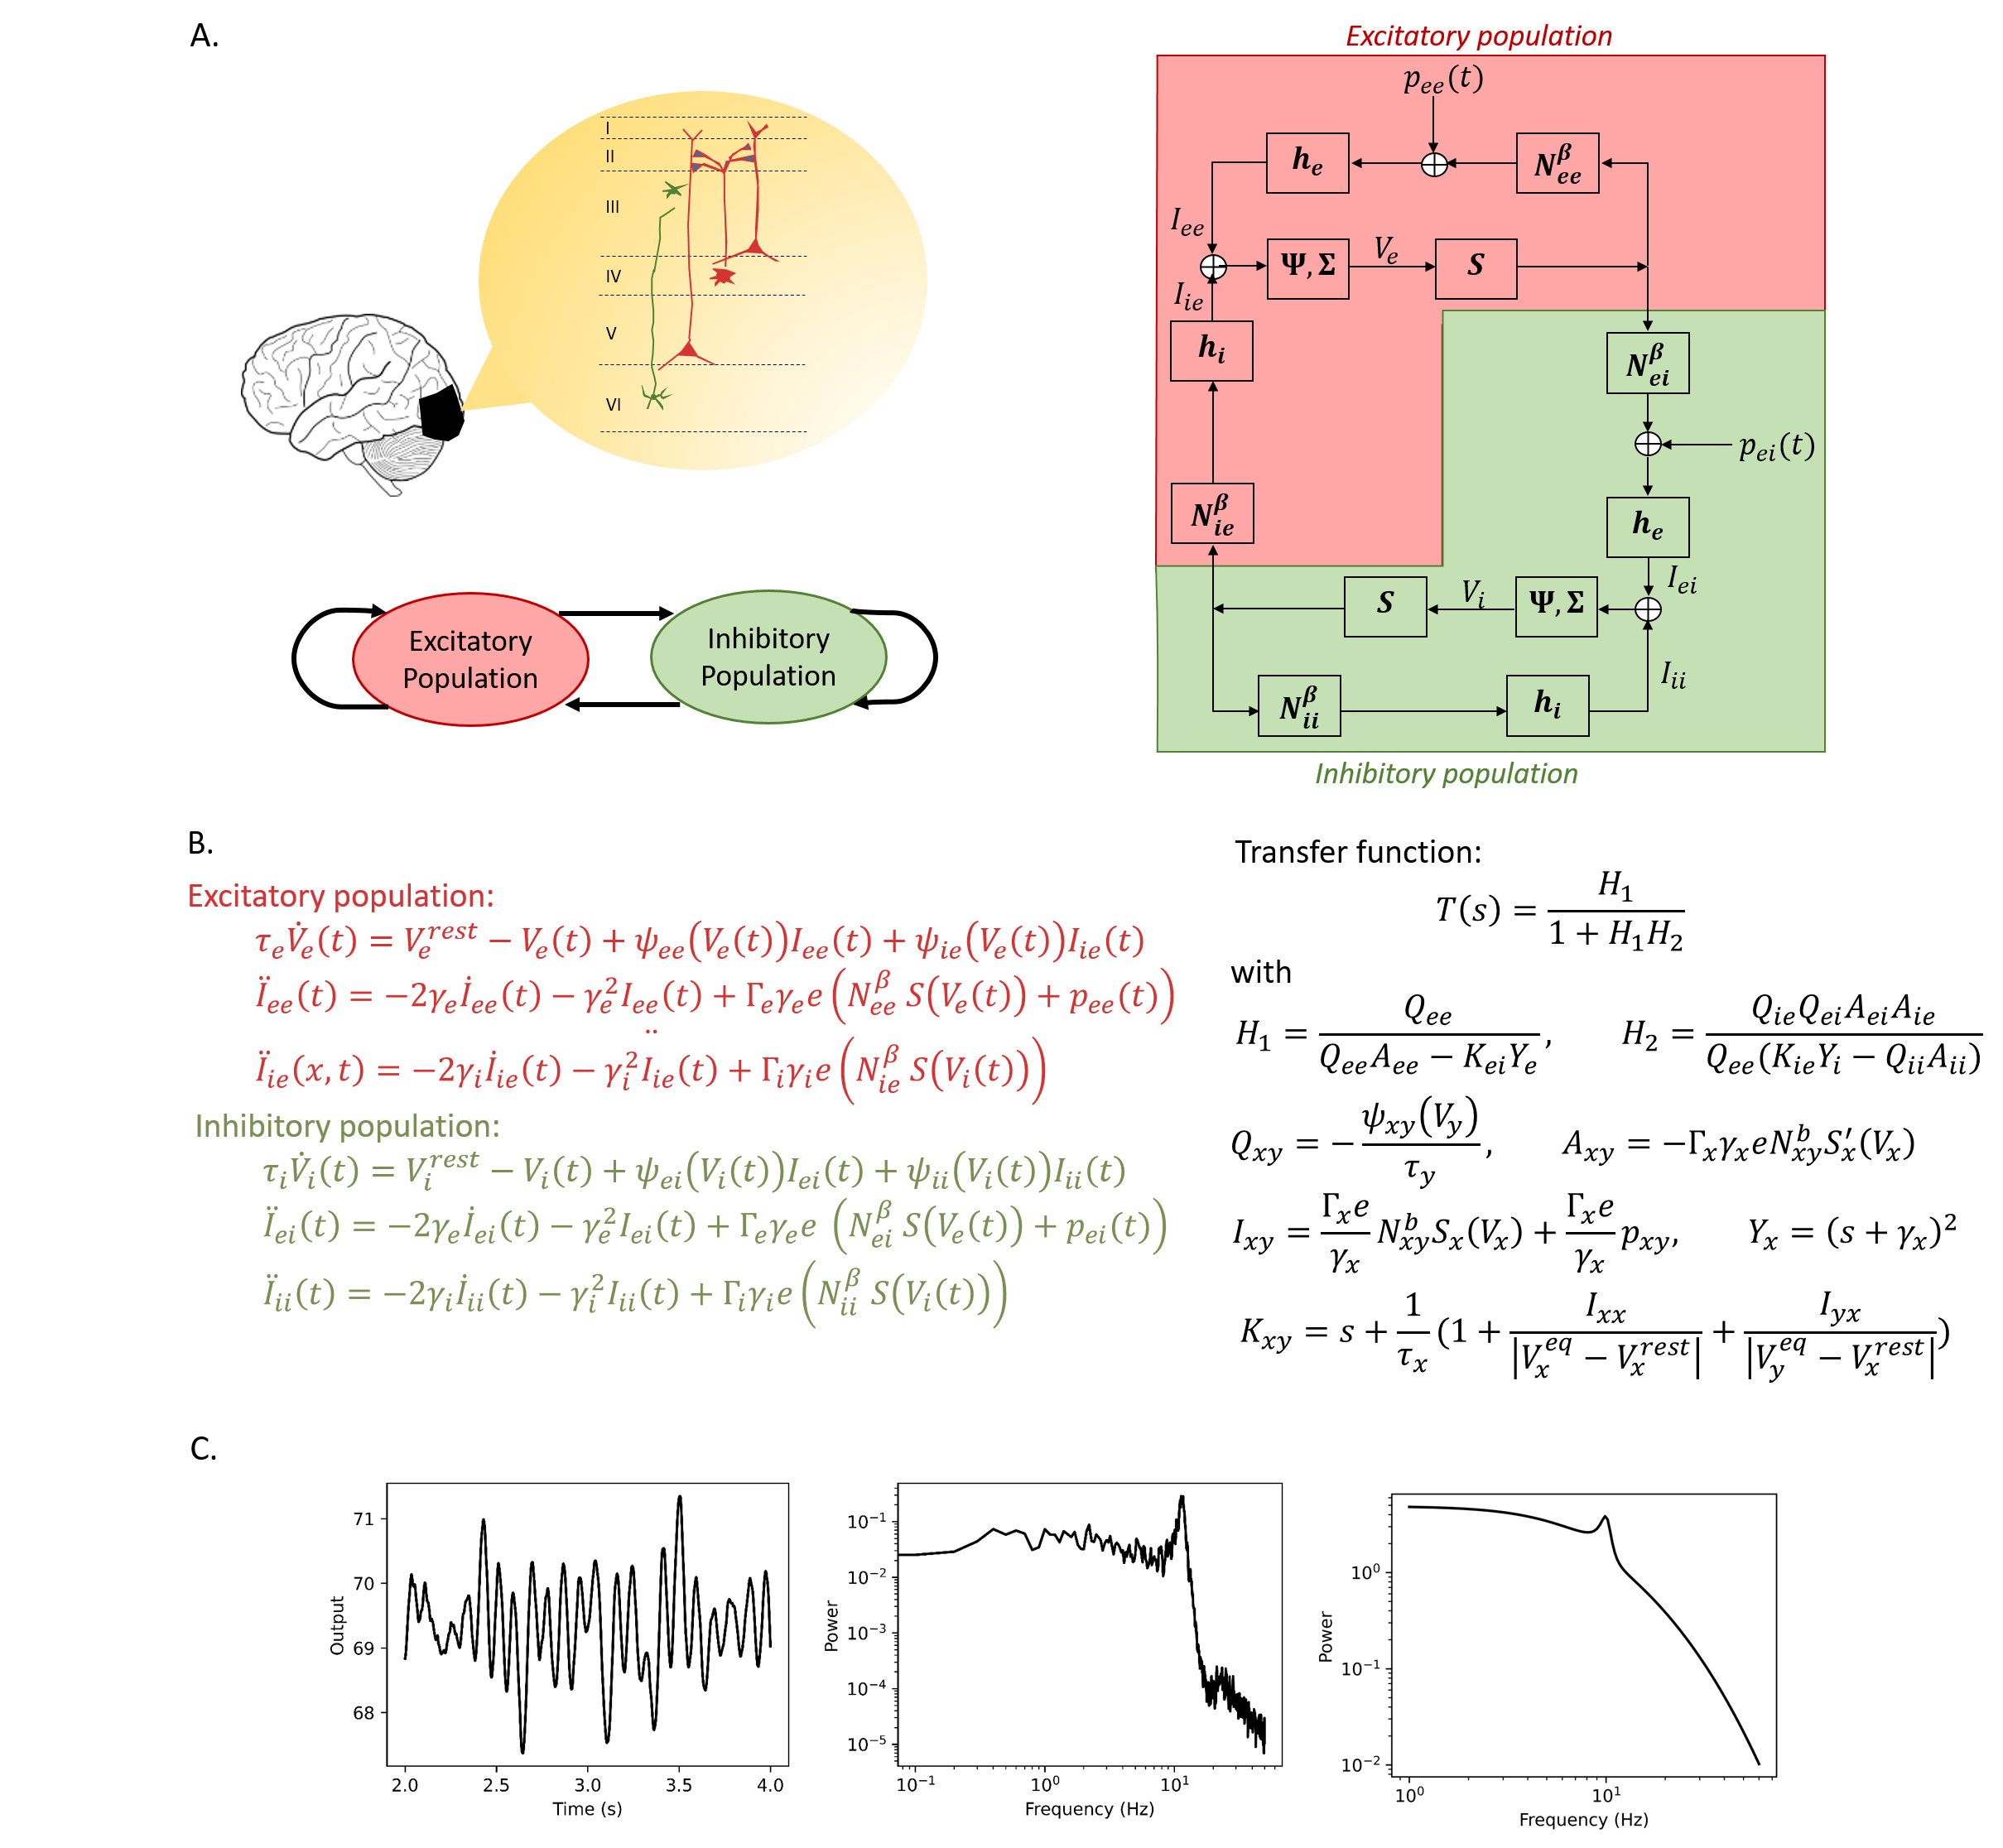
\includegraphics[scale=0.48]{Images/Liley_schematic_2.png}
    \caption*{\textbf{Figure 7. \textit{LW model  topography, schematic, numerical and analytical mathematical expression, and alpha simulation results.}} \textbf{A)} The general structure of the model is two neural populations each with a self-connection. In the detailed schematic, compared to the other models, a third block is introduced to transform PSP into soma membrane potential. \textbf{B)} Left: Numerical mathematical expression for each neural population; Right: Transfer function of the model derived using control graph analysis; \textbf{C)} Simulation outputs of the model with standard parameters (time series, power spectrum estimated from the time series and analytical power spectrum)
    }        
    \label{fig:Lil_topography}
\end{figure}
%TC:endignore


%\begin{figure}[H]
 %   \hspace{-0.5cm}
  %  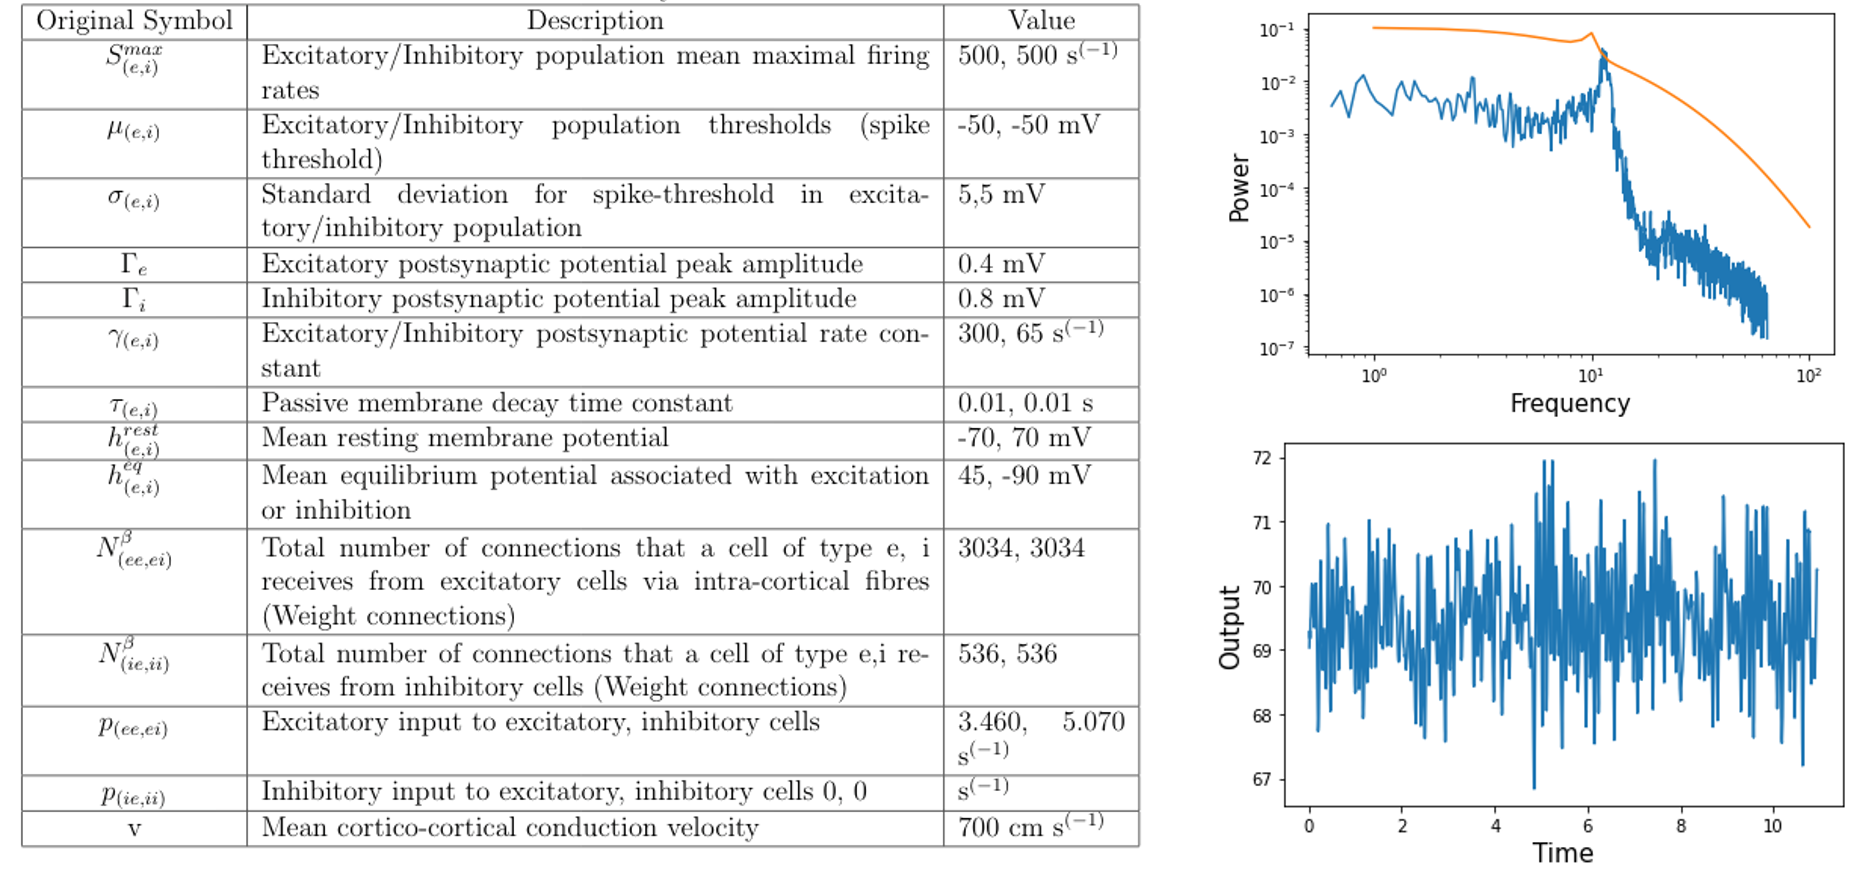
\includegraphics[scale=0.55]{Images/Lil_oscillations.png}
   % \caption*{\textbf{Figure 4.  \textit{LW time series and corresponding power spectrum for standard parameter values of alpha oscillations}}. Table with standard parameter values; Time series for 3 seconds and power spectrum with distinctive alpha peak}
   % \label{fig:LW_oscillation}
%\end{figure}
% \begin{figure}[H]
%     \centering
%     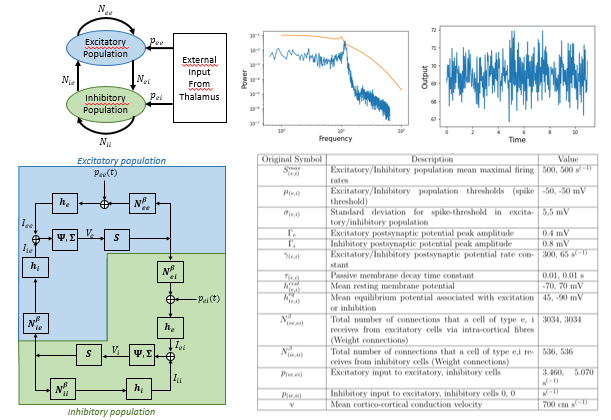
\includegraphics[scale=0.9]{Images/test_lil.png}
%     \caption*{\textbf{Figure 8.  \textit{LW model topography and detailed schematic of two neural population.}} Two neural population represented each with a self-connection. In the detailed, schematic we notice a third block to transform PSP into soma membrane potential.%Add more description... 
%     }        
%     \label{fig:Lil_topography}
% \end{figure}

%TC:ignore
\subsubsection{Robinson-Rennie-Wright model}
%TC:endignore
% From cook: To investigate the spatially uniform activity, the spatially inhomogeneous term in the wave equation Eq. (4.20) is set to zero.  To make this a neural mass model, we would set the axonal range to zero rb = 0.  However, setting ∇ 2φ b(x,t) = 0 allows us to solve for the spatially uniform solutions of the neural field model.  This removes the spatial variation while still preserving the axonal range, conduction velocity and intra-cortical connectivities.

Unlike the three models discussed thus far, the RRW model does not attempt to offer a minimal circuit representation of a single cortical macrocolumn. Instead, this model includes thalamic neural populations in addition to cortical ones, and thus is primarily concerned with describing cortico-thalamic interactions. RRW permits the exploration of the second class of alpha theory outlined in Fig. 2B, which hypothesize that the corticothalamic loop is central for resting state alpha. The model consists of four neural populations, two cortical (excitatory and inhibitory, similar to previous schematics) and two thalamic (thalamic reticular nucleus and thalamic relay nuclei) \citep{robinson2002dynamics}. In this case, the two cortical populations are lumped together by assuming that intracortical connections are random, making their number proportional to the number of available synapses, and implying that cortical excitatory and inhibitory voltages are equal \citep{roberts2012corticothalamic}. As noted above, like LW the original formulation of RRW is as a neural field model, making use of a damped wave equation operator for including a spatial representation. However, here we again assume spatial uniformity, removing any spatial variations, as indeed is commonly done in analyses of this model. Propagation delay and long axonal ranges are still preserved solely for the cortical excitatory population, this being the only population large enough with distant connections for wave propagation to have a significant effect \citep{zhao2015slow}. 
Furthermore, a corticothalamic loop delay parameter ($t_0$) is introduced in the model to take into account the conduction delay of the signal when it passes through thalamic nuclei and the projections.
The differential equations comprising the RRW model version we use here are explicitly detailed by \citet{zhao2015generalized}, who also modified them to study epileptic seizures and bursting dynamics. The firing rate is defined as 

\begin{equation}
    Q_a=\frac{Q_a^{max}}{1+e^{-\frac{V_a-\theta_a}{\sigma_a'}}}
\end{equation}

with $Q_{max}$ representing the maximum firing rate, $\theta_{a}$ the mean firing threshold, and $\sigma_a'\pi \sqrt{3}$ the standard deviation of the threshold distribution. The damped wave equation governing long-range axonal activity propagation is expressed as

\begin{equation}
    D_a \phi_a=Q_a
\end{equation}

with $\phi_a$ corresponding to the mean density of outgoing spikes produced by population $a$ and $D_a=\frac{1}{\gamma_a^2} \frac{\partial^2}{\partial t^2}+ \frac{2}{\gamma_a} \frac{\partial}{\partial t} + 1- r_a^2 \nabla^2$ \\

In the spatially uniform case where $\nabla^2=0$, owing to the short range of cortical inhibitory axons and the relative smallness of the thalamus, $\gamma_a$ is so large that the approximation $\phi_a=Q_a$ can be made for $a=i,r,s$. This is called the \textit{local interaction approximation} and is not assumed for $\phi_e$ as the propagation effects are significant only when considering the axons of the excitatory cortical neurons, as they are the only ones with sufficient length as mentioned previously \citep{robinson2001prediction, robinson2002dynamics, sanz2017multistability}.

The impulse response in RRW includes both synaptic rise time $\beta^{-1}$ and synaptic decay time $\alpha^{-1}$ parameters, and is defined as

\begin{equation}
    \begin{aligned}
    w(u) &=\frac{\alpha \beta}{\beta - \alpha}(e^{-\alpha u} - e^{-\beta u}) \quad \text{for } \beta \neq \alpha \\
    w(u) &= \alpha ^{2}ue^{-\alpha u} \quad \text{for } \alpha = \beta
    \end{aligned}
\end{equation}

which implies that the dendritic response is

\begin{equation}
    D_{\alpha \beta} =  \frac{1}{\alpha \beta}  \frac{d^2}{dt^2}+\left(\frac{1}{\alpha}+\frac{1}{\beta}\right) \frac{d}{dt}+1
\end{equation}

which is identical to the JR impulse response function when $\alpha = \beta$. In the spatially uniform case, the impulse response appears as 

\begin{eqnarray}
    D_{\alpha \beta} V_e (t) &=& v_{ee} \phi_e (t)+v_{ei} \phi_i (t)+v_{es} \phi_s (t-t_0/2) \\
    D_{\alpha \beta} V_r (t) &=& v_{re} \phi_e (t-t_0 /2)+v_{rs} \phi_s (t) \\
    D_{\alpha \beta} V_s (t) &=& v_{se} \phi_e (t-t_0 /2)+v_{sr} \phi_r (t)+v_{sn} \phi_n (t)
\end{eqnarray}

%TC:ignore
\begin{figure}[H]
    \centering
    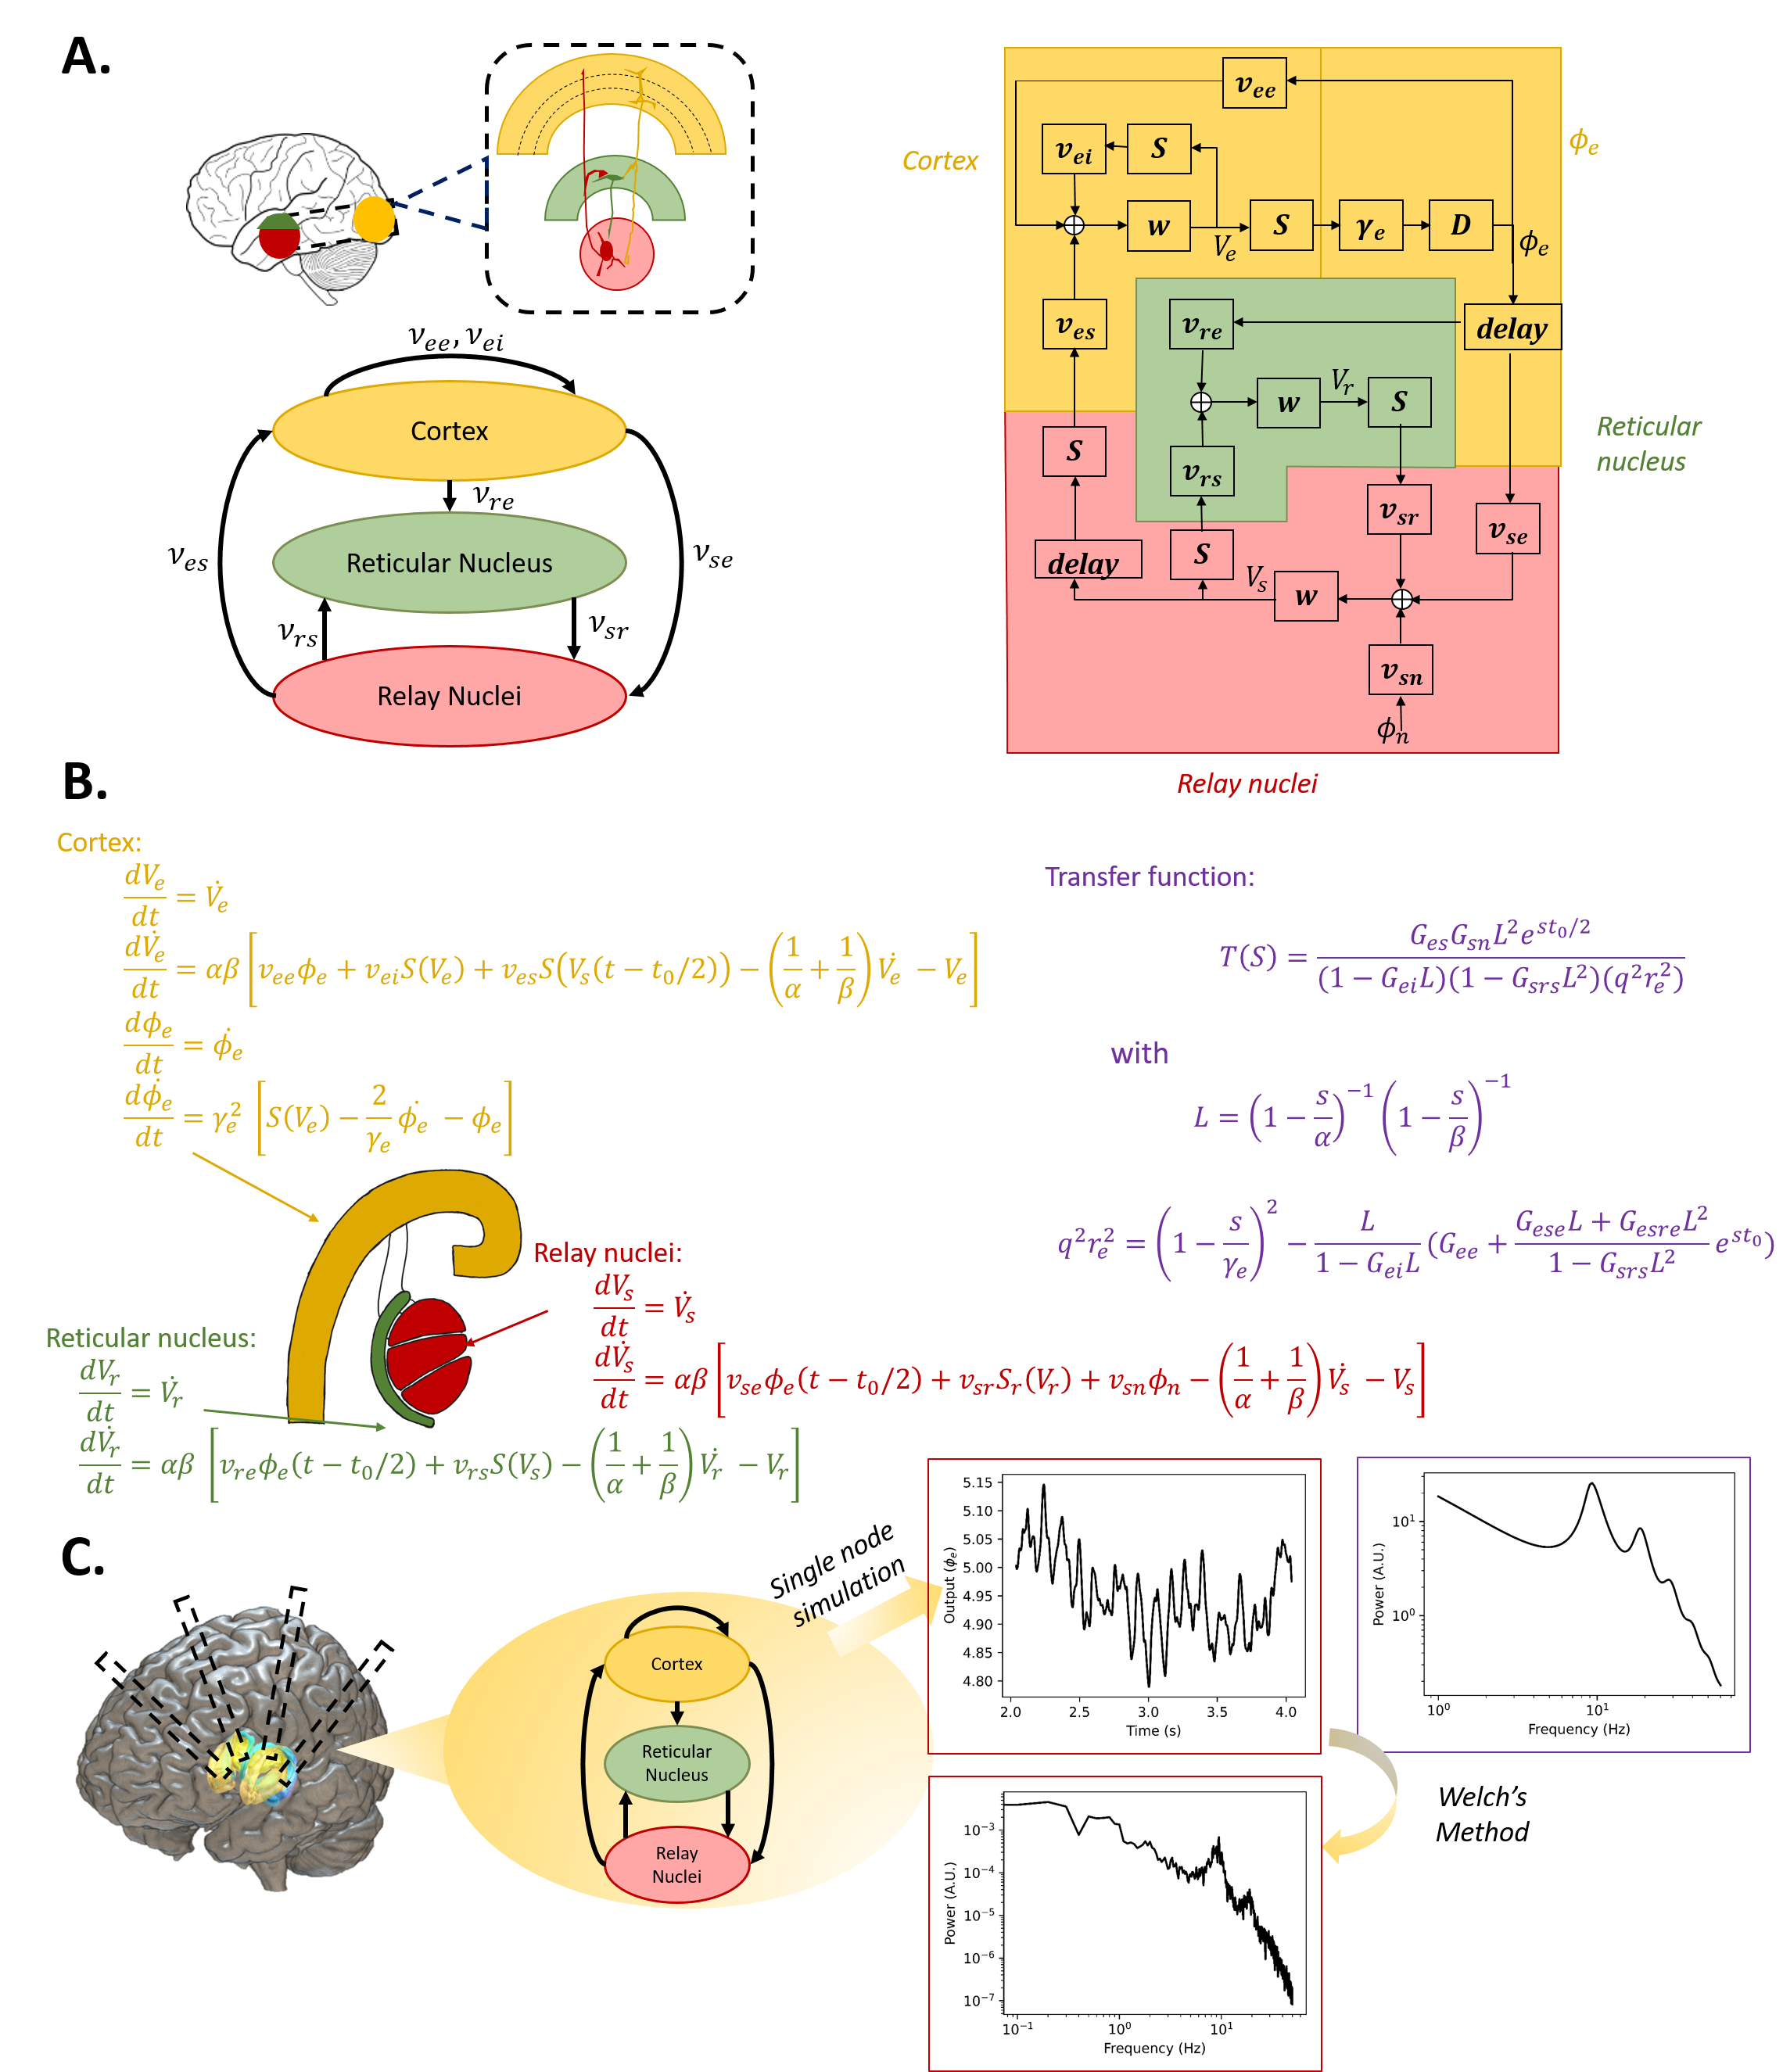
\includegraphics[scale=0.45]{Images/Robinson_schematic_4.png}
    %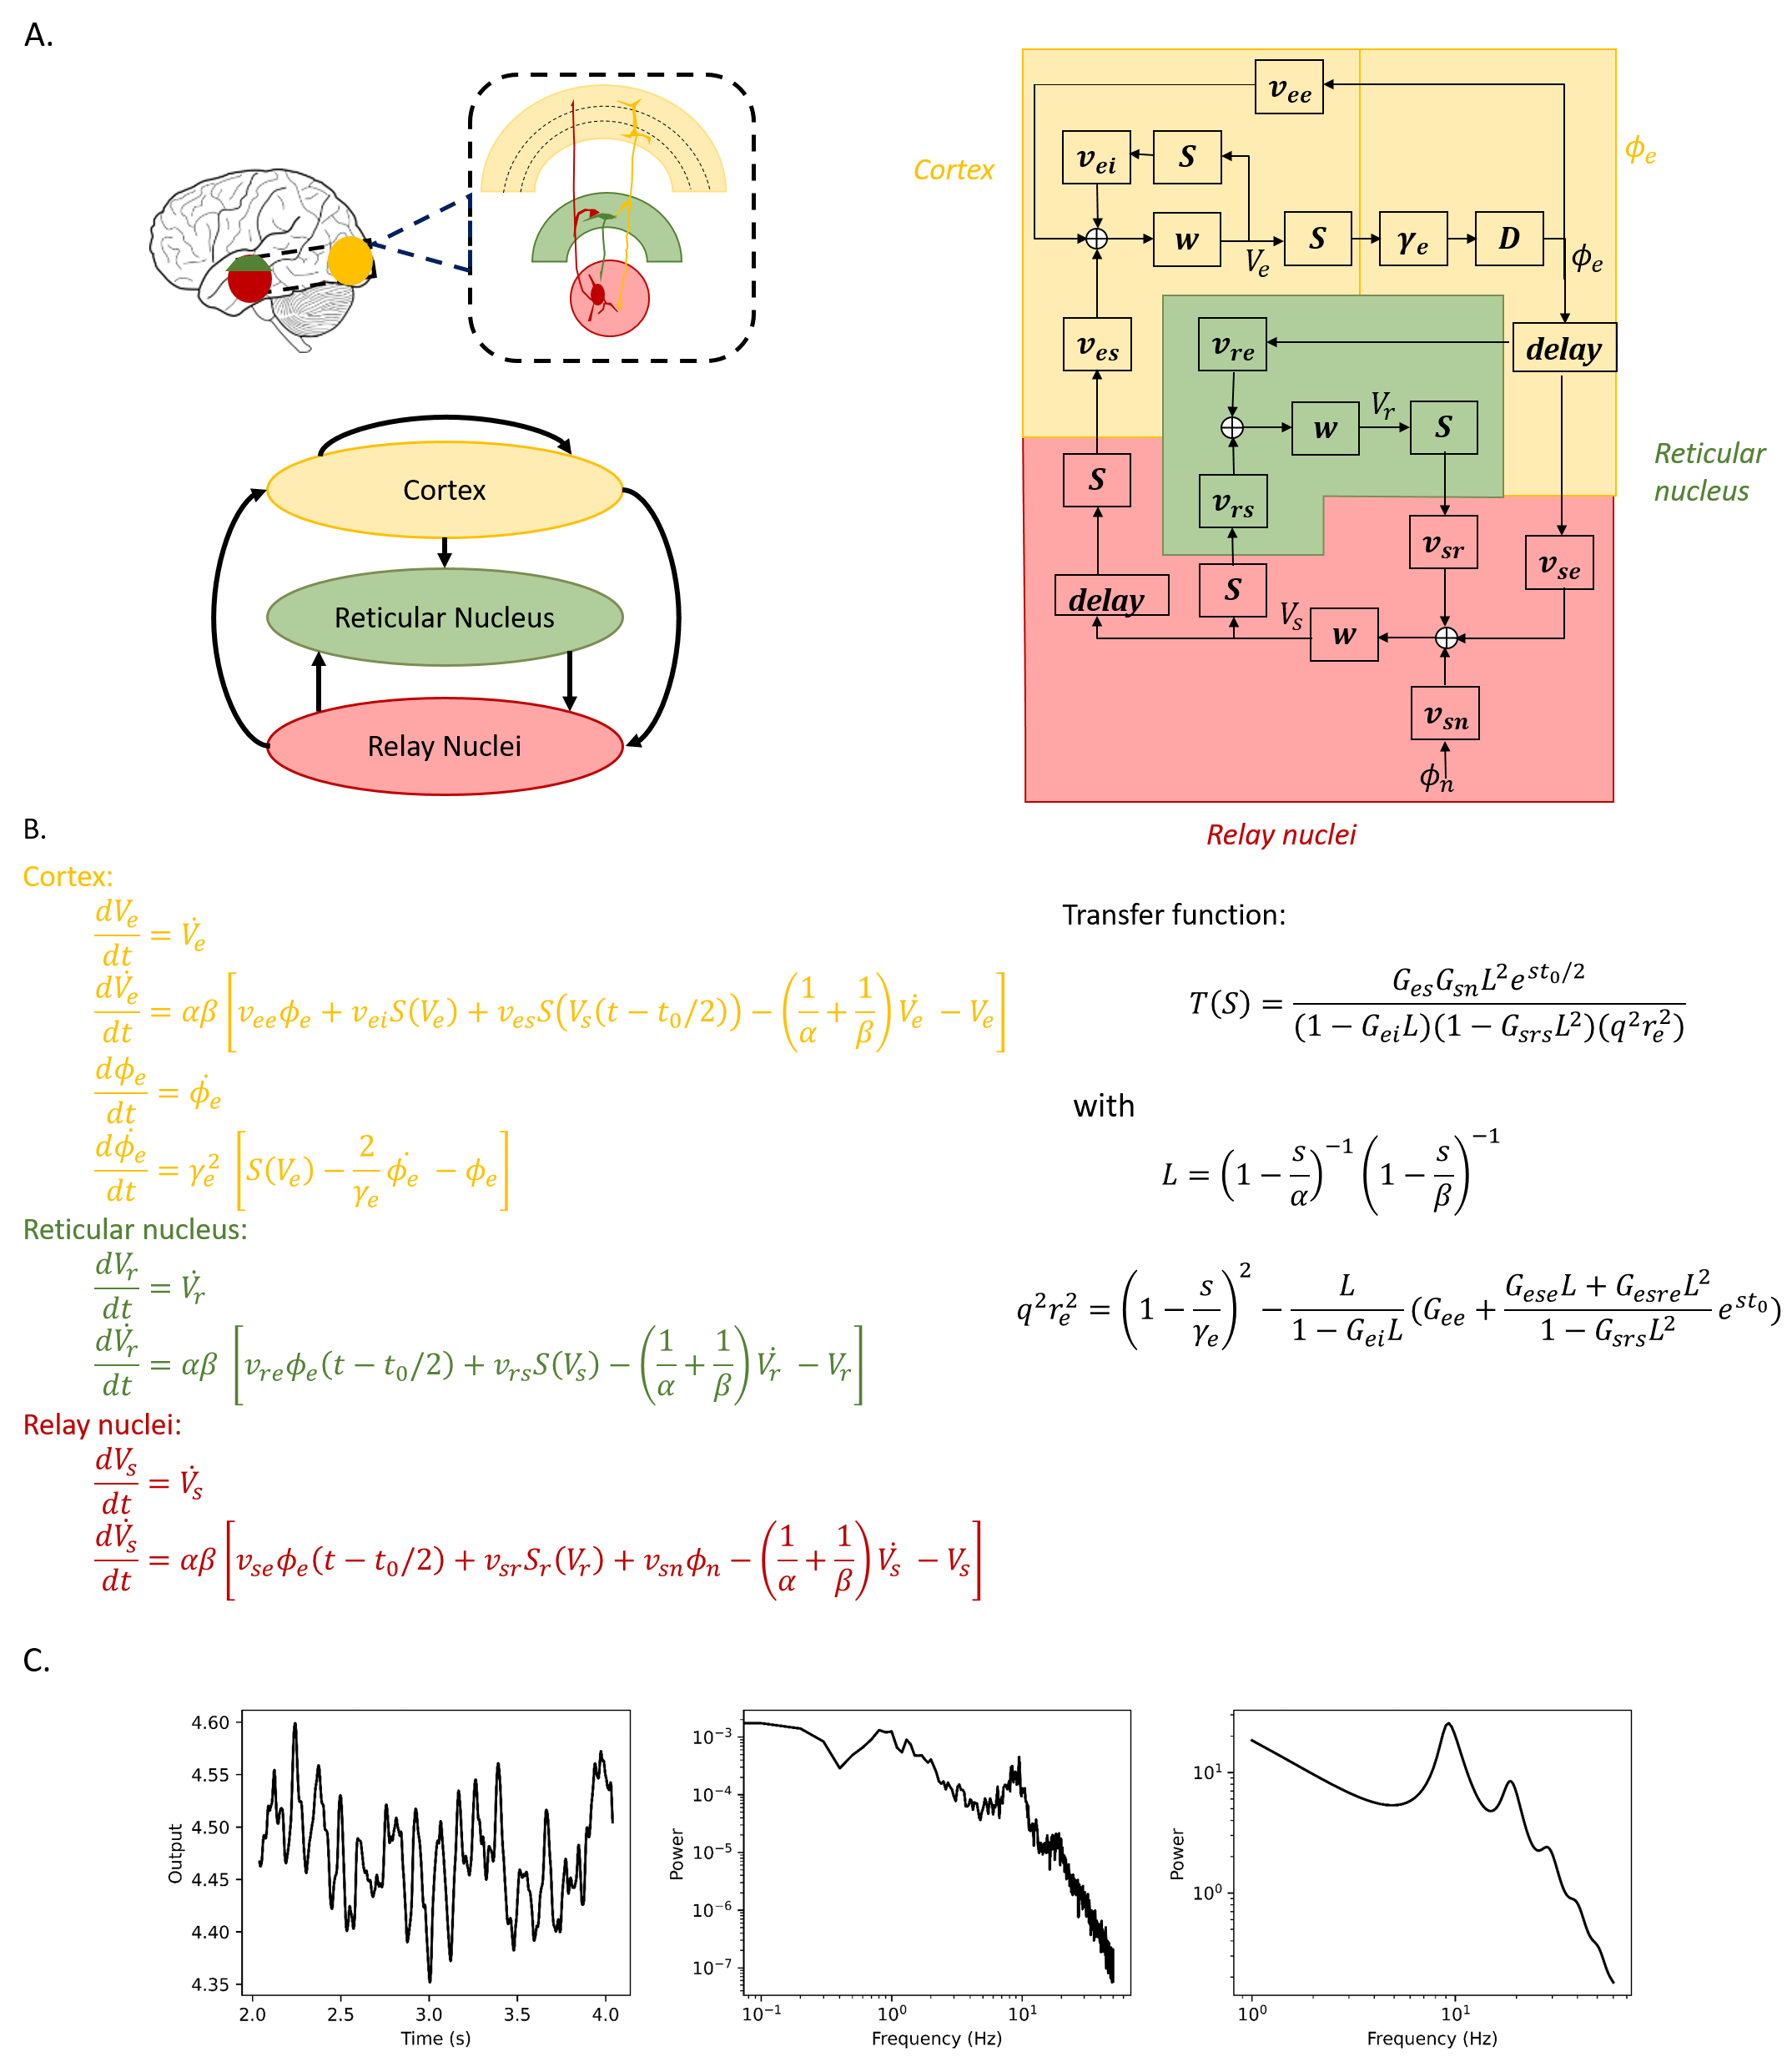
\includegraphics[scale=0.48]{Images/Robinson_schematic_3.png}
    \caption*{\textbf{Figure 8.  \textit{RRW model topography, schematic, numerical and analytical mathematical expression, and alpha simulation results.}} \textbf{A)} Three main populations are broadly described: the cortex (composed of excitatory and inhibitory neurons) and two thalamic populations (reticular nucleus and relay nuclei). Delays are included to take into account long range connections from the cortex to the thalamus; \textbf{B)} Left: Numerical mathematical expression for each neural population; Right: Transfer function of the model derived using control graph analysis; \textbf{C)} Simulation outputs of the model with standard parameters (time series, power spectrum estimated from the time series and analytical power spectrum)}            
    \label{fig:Rob_topography}
\end{figure}
%TC:endignore


%\begin{figure}[H]
 %   \hspace{-0.48cm}
  %  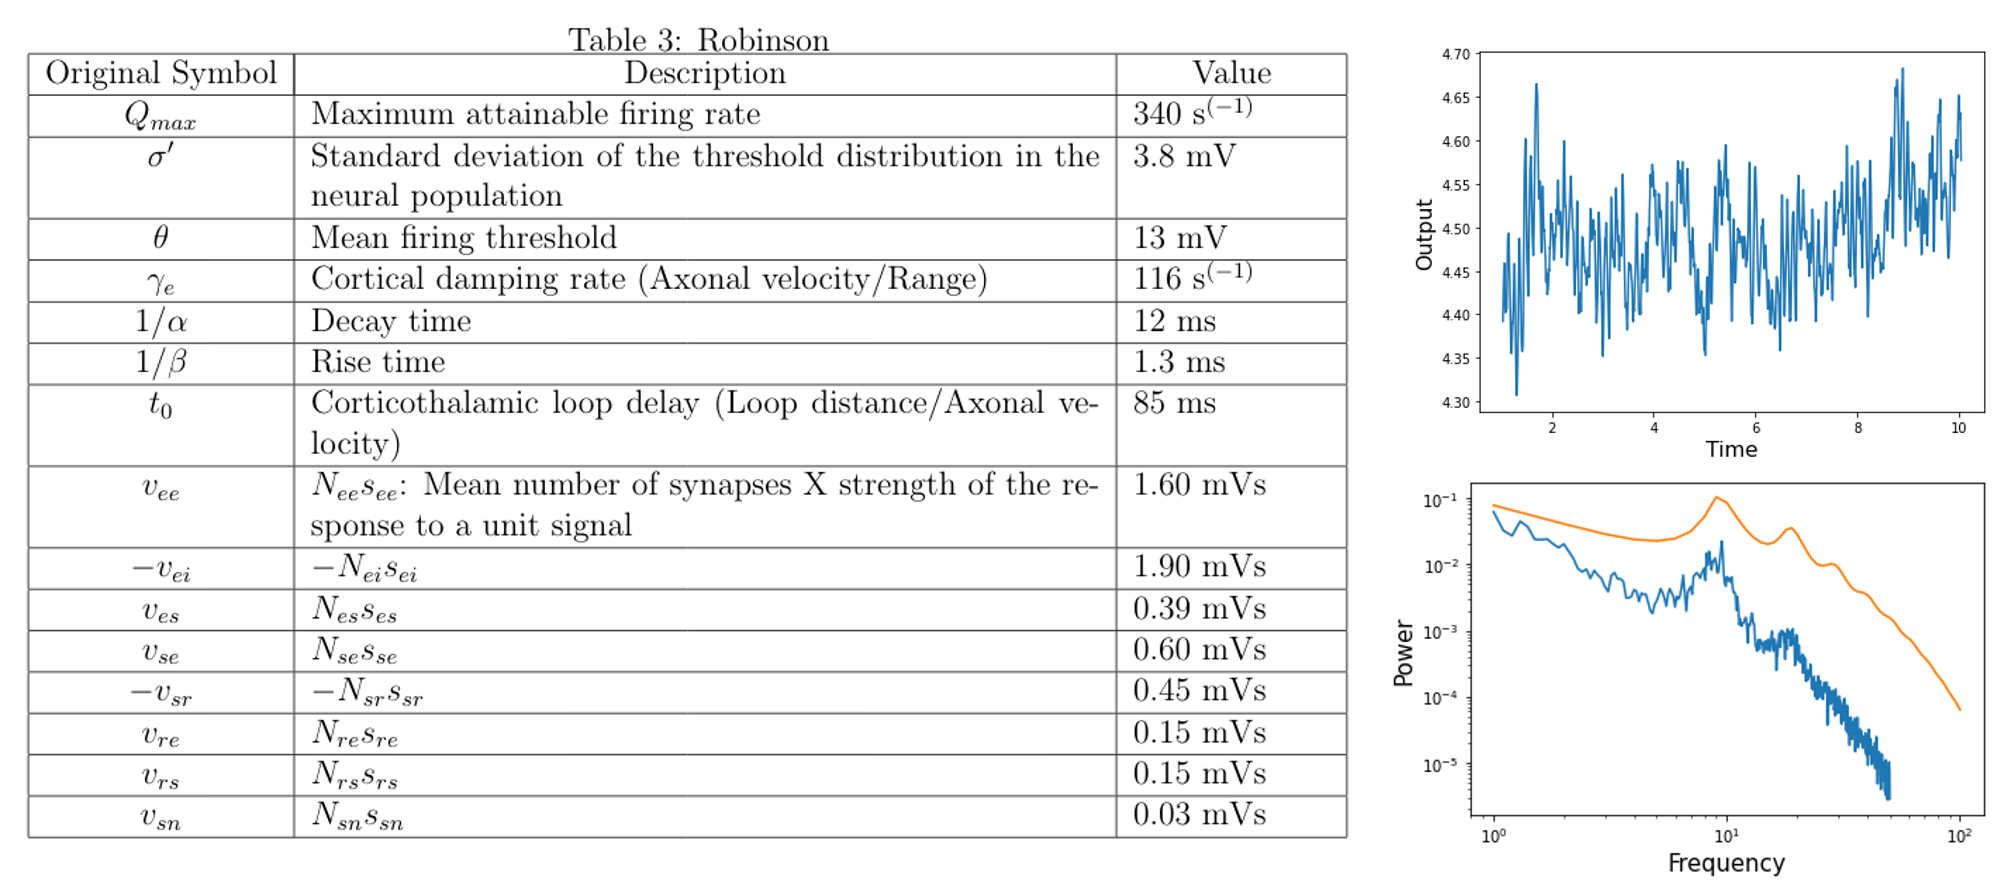
\includegraphics[scale=0.52]{Images/Rob_oscillations.png}
   % \caption*{\textbf{Figure 4.  \textit{RWW time series and corresponding power spectrum for standard parameter values of alpha oscillations}}. Table with standard parameter values; Time series for 3 seconds and power spectrum with distinctive alpha peak}
    %\label{%fig:RWW_oscillation}
%\end{figure}




% Zhao (put) explicitely layed out the formulation of the differential equation expression with modifications to simulate seizured. Here after is the expression without seizure an thus the RRW equivalent.
% \begin{align*}
%     \frac{dV_e}{dt} &= \dot{V_e} \\
%     \frac{d\dot{V_e}}{dt} &= \alpha \beta[v_{ee} \phi_e+v_{ei} S(V_e)+v_{es} S(V_s (t-t_0/2))-(\frac{1}{\alpha} + \frac{1}{\beta}) \dot{V_e} - V_e ] \\
%     \frac{dV_r}{dt} &= \dot{V_r} \\
%     \frac{d\dot{V_r}}{dt} &= \alpha \beta [v_{re} \phi_e (t-t_0/2)+v_{rs} S(V_s )-(\frac{1}{\alpha}+\frac{1}{\beta}) \dot{V_r}-V_r ] \\
%     \frac{dV_s}{dt} &= \dot{V_s} \\
%     \frac{d\dot{V_s}}{dt} &= \alpha \beta [v_{se} \phi_e (t-t_0/2)+v_{sr} S_r(V_r )+v_{sn} \phi_n-(\frac{1}{\alpha}+\frac{1}{\beta}) \dot{V_s}-V_s ] \\
%     \frac{d\phi_e}{dt} &= \dot{\phi_e} \\
%     \frac{d\dot{\phi_e}}{dt} &= \gamma_e^2  [S(V_e)-\frac{2}{\gamma_e}  \dot{\phi_e}-\phi_e ]
% \end{align*}

% Robinson et al. performed many analysis using a linearized expression which is the following:\\

% \begin{align*}
%     L &=\left(1-\frac{s}{\alpha}\right)^{-1}\left(1-\frac{s}{\beta}\right)^{-1} \\
%     q^2 r^2&=\left(1-\frac{s}{\gamma_e}\right)^2-\frac{1}{1-G_{ei} L}\left(G_{ee} L+\frac{(G_{ese} L^2+G_{esre} L^3)e^{st_0}}{1-G_{srs} L^2 }\right)\\
%     term_1 &=\frac{\phi_n^2}{4\pi r_e^4}\\
%     term_2 &=\left|\frac{(G_{esn} L^2)}{(1-G_{srs} L^2 )(1-G_{ei} L)}\right|^2\\
%     term_3 &=\left|\frac{Arg \; q^2}{Im \; q^2} \right|\\
%     P(w) &=term_1 \times term_2 \times term_3 
% \end{align*}


% Can mention Cook again for explicit derivation of the equations 

%TC:ignore
\subsection{Simulation, power spectrum, and stability analysis methods}
%TC:endignore
For all four of the selected models, we simulate alpha activity numerically (by integrating the models' differential equations given in Figs. 5-8 and Supplementary S.6) and analytically, by algebraically calculating the power spectrum from the models' transfer function. Python is utilized as the programming language for implementing all numerical and analytical equations, as well as statistical analyses and visualization. To ensure consistency, simulations are executed for a duration of 100 seconds, generating a time series that represents neural activity within the principal excitatory cortical population. The power spectrum of this simulated activity is then computed using Welch's method, as implemented in the scipy library \citep{2020SciPy-NMeth}. 

The ability and accuracy of the models to replicate an empirical alpha rhythm is explored by running numerical simulations with parameter values that are commonly used in previous studies to elicit alpha activity, which we refer to as `standard alpha parameters'. The resulting power spectra are compared against characteristic empirical resting state EEG features. These nominal parameter values are taken from \citet{jansen1995electroencephalogram} for JR, \citet{moran2007neural} for MDF (using \citet{david2003neural} to tune to a dominant frequency of alpha [8-12Hz] instead of beta [12-20Hz]), \citet{liley2001spatially} for LW, and \citet{zhao2015generalized} for RRW, which stem from \citet{robinson2002dynamics, rowe2004estimation}. Defining precise reference features of empirical alpha rhythms presents a challenge, due to the observed heterogeneity in resting state alpha oscillations both within individuals and between individuals across different moments \citep{niedermeyer2005normal}. However, certain prominent elements of the resting state power spectral density are well-established. On average, a healthy adult human exhibits a main oscillation frequency near 10Hz, accompanied by the presence of harmonics \citep{van2010neurophysiological}. These features are considered somewhat volatile, as they significantly vary between individuals and across different sessions. More stable or broader resting state EEG features include: the frequency scaling of $1/f^{\beta}$ ($\beta \approx 1 - 2$) \citep{muthukumaraswamy20181}, and the phenomenon of \textit{alpha blocking} - attenuation of the alpha frequency peak during the transition from eyes-closed (EC) to eyes-open (EO) state. Each model's estimation of these features is compared against reference values derived from empirical data for evaluation, more specifically from \citet{muthukumaraswamy20181} where they used Irregularly Resampled Auto Spectral Analysis to quantify the 1/f components of MEG/EEG/ECoG data. The high and low frequency $\beta$ values were obtained from 5min 64 channel EEG eyes-closed recordings of seventeen healthy male participants (mean age = 23), and results were confirmed with other datasets \citep{muthukumaraswamy20181}. 

The $\beta$ frequency scaling can be quantified in several ways. One approach involves considering the entire spectrum, which empirically tends to fall within the range of 1 to 2. Another approach involves evaluating two distinct values of $\beta$, one for lower frequencies (pre-peak) and another for higher frequency values (post-peak). In our simulated results, we estimated $\beta$ with two different methods: 1) Evaluating pre- and post-peak $\beta$ separately by fitting a line with linear regression in the logarithmic scale, and 2) Using the power spectrum fit of the FOOOF library (https://fooof-tools.github.io/fooof/; \citealp{donoghue2020parameterizing}), which parametrizes neural power spectra into a mixture of the $1/f^\beta$ background and a Gaussian for each frequency peak. These FOOOF fits are also used to calculate the dominant oscillation frequencies of the power spectra, which are discussed in detail in parameter space figures of Section 3.1.2. We compare the $\beta$ values approximated for each of our models against those estimated from EO and EC resting state EEG data reported in \citet{muthukumaraswamy20181}. All signal processing analysis and modelling results are fully available at https://github.com/GriffithsLab/Bastiaens2024\_AlphaModels and implemented in Python 3.8. 

To gain further insights into the dynamics generated by JR and LW, we determined the stability of the fixed points of the system as a function of E-I connection strengths. \\
For JR, similar to \citet{grimbert2006bifurcation}, the fixed points are determined by setting the derivatives to 0. With some manipulations, the equilibrium points in the ($C, y_1 - y_2$) plane with $y = y_1 - y_2$ are equal to:

\begin{equation}
    y = \frac{A}{a}p + \frac{A}{a}C_2S(\frac{A}{a}C_1S(y) - \frac{B}{b}C_4S(\frac{A}{a}C_3S(y))
\end{equation}

The stability of the fixed points is then defined using the Jacobian matrix

\[
\hspace{-1cm}
\mathbf{Y}_{i,j} =
\begin{bmatrix}
  \frac{\partial y_0}{\partial y_0} & 
    \frac{\partial y_0}{\partial y_1} & 
    \frac{\partial y_0}{\partial y_2} &
    \frac{\partial y_0}{\partial y_3} &
    \frac{\partial y_0}{\partial y_4} &
    \frac{\partial y_0}{\partial y_5 } \\[1ex] % <-- 1ex more space between rows of matrix
  \frac{\partial y_1}{\partial y_0} & 
    \frac{\partial y_1}{\partial y_1} & 
    \frac{\partial y_1}{\partial y_2} &
    \frac{\partial y_1}{\partial y_3} &
    \frac{\partial y_1}{\partial y_4} &
    \frac{\partial y_1}{\partial y_5 } \\[1ex]
  \frac{\partial y_2}{\partial y_0} & 
    \frac{\partial y_2}{\partial y_1} & 
    \frac{\partial y_2}{\partial y_2} &
    \frac{\partial y_2}{\partial y_3} &
    \frac{\partial y_2}{\partial y_4} &
    \frac{\partial y_2}{\partial y_5 } \\[1ex]
  \frac{\partial y_3}{\partial y_0} & 
    \frac{\partial y_3}{\partial y_1} & 
    \frac{\partial y_3}{\partial y_2} &
    \frac{\partial y_3}{\partial y_3} &
    \frac{\partial y_3}{\partial y_4} &
    \frac{\partial y_3}{\partial y_5 } \\[1ex] 
  \frac{\partial y_4}{\partial y_0} & 
    \frac{\partial y_4}{\partial y_1} & 
    \frac{\partial y_4}{\partial y_2} &
    \frac{\partial y_4}{\partial y_3} &
    \frac{\partial y_4}{\partial y_4} &
    \frac{\partial y_4}{\partial y_5 } \\[1ex]
  \frac{\partial y_5}{\partial y_0} & 
    \frac{\partial y_5}{\partial y_1} & 
    \frac{\partial y_5}{\partial y_2} &
    \frac{\partial y_5}{\partial y_3} &
    \frac{\partial y_5}{\partial y_4} &
    \frac{\partial y_5}{\partial y_5 } 
\end{bmatrix}
= 
\begin{bmatrix}
  0 & 
    0 & 
    0 &
    1 &
    0 &
    0 \\[1ex] % <-- 1ex more space between rows of matrix
  0 & 
    0 & 
    0 &
    0 &
    1 &
    0 \\[1ex]
  0 & 
    0 & 
    0 &
    0 &
    0 &
    1 \\[1ex]
  -a^2 & 
    AaS'(y) & 
    -AaS'(y) &
    -2a &
    0 &
    0 \\[1ex]
  AaC_{2}C_{1}S'(C_{1}y_0(y)) & 
    -a^2 & 
    0 &
    0 &
    -2a &
    0 \\[1ex]
  BbC_{4}C_{3}S'(C_{3}y_0(y)) & 
    0 & 
    -b^2 &
    0 &
    0 &
    -2b
\end{bmatrix}
\]
with $y$ corresponding to the fixed point of interest and $y_0(y) = \frac{A}{a}S(y)$. Stability is then defined by calculating the eigenvalues of the matrix $\mathbf{Y}$ for each fixed point, and looking at the sign of the real part of the eigenvalues. The system is stable if all the eigenvalues have a negative real part. If at least one of the eigenvalues has a positive real part, it is considered as an unstable fixed point. 

Using a similar method (estimation of the fixed point, following an assessment of the stability of the fixed points by looking at the real part of the eigenvalues of the Jacobian matrix), the LW equilibrium points' stability was also determined. The full calculation and equations are detailed in the appendix of \citet{hartoyo2019parameter} and also in Supplementary S.6. Briefly: 

The equilibrium point equations can be reduced to:
\begin{eqnarray}
    0 &=& -V_e + V_{er} + \psi_{ee}(V_e)I_{ee} + \psi_ie(V_e)I_{ie} \\
    0 &=& -V_i + V_{ir} + \psi_{ei}(V_i)I_{ei} + \psi_{ii}(V_i)I_{ii}
\end{eqnarray}
with
\begin{eqnarray}
    I_{ee} &=& \frac{\Gamma_ee}{\gamma_e}N_{ee}^{\beta}S(V_e) + \frac{\Gamma_ee}{\gamma_e}p_{ee} \\
    I_{ei} &=& \frac{\Gamma_ee}{\gamma_e}N_{ei}^{\beta}S(V_e) + \frac{\Gamma_ee}{\gamma_e}p_{ei} \\
    I_{ie} &=& \frac{\Gamma_ie}{\gamma_i}N_{ie}^{\beta}S(V_i) + \frac{\Gamma_ie}{\gamma_i} \\
    I_{ii} &=& \frac{\Gamma_ie}{\gamma_i}N_{ii}^{\beta}S(V_i) + \frac{\Gamma_ie}{\gamma_i}
\end{eqnarray}

The fixed points for $V_e$ and $V_i$ are then estimated by finding the values for which values these two equations intersect.

The Jacobian matrix is: 

\[
\mathbf{F}_{i,j} =
\begin{bmatrix}
  \frac{\partial V_e}{\partial V_e} & 
    \frac{\partial V_e}{\partial V_i} & 
    \frac{\partial V_e}{\partial I_{ee}} &
    \frac{\partial V_e}{\partial I_{ei}} &
    \frac{\partial V_e}{\partial I_{ie}} &
    \frac{\partial V_e}{\partial I_{ii}} &
    \frac{\partial V_e}{\partial U_{ee}} &
    \frac{\partial V_e}{\partial U_{ei}} &
    \frac{\partial V_e}{\partial U_{ie}} &
    \frac{\partial V_e}{\partial U_{ii}} \\[1ex] % <-- 1ex more space between rows of matrix
  \frac{\partial V_i}{\partial V_e} & 
    \frac{\partial V_i}{\partial V_i} & 
    \frac{\partial V_i}{\partial I_{ee}} &
    \frac{\partial V_i}{\partial I_{ei}} &
    \frac{\partial V_i}{\partial I_{ie}} &
    \frac{\partial V_i}{\partial I_{ii}} &
    \frac{\partial V_i}{\partial U_{ee}} &
    \frac{\partial V_i}{\partial U_{ei}} &
    \frac{\partial V_i}{\partial U_{ie}} &
    \frac{\partial V_i}{\partial U_{ii}} \\[1ex]
  \frac{\partial I_{ee}}{\partial V_e} & 
    \frac{\partial I_{ee}}{\partial V_i} & 
    \frac{\partial I_{ee}}{\partial I_{ee}} &
    \frac{\partial I_{ee}}{\partial I_{ei}} &
    \frac{\partial I_{ee}}{\partial I_{ie}} &
    \frac{\partial I_{ee}}{\partial I_{ii}} &
    \frac{\partial I_{ee}}{\partial U_{ee}} &
    \frac{\partial I_{ee}}{\partial U_{ei}} &
    \frac{\partial I_{ee}}{\partial U_{ie}} &
    \frac{\partial I_{ee}}{\partial U_{ii}} \\[1ex]
  \frac{\partial I_{ei}}{\partial V_e} & 
    \frac{\partial I_{ei}}{\partial V_i} & 
    \frac{\partial I_{ei}}{\partial I_{ee}} &
    \frac{\partial I_{ei}}{\partial I_{ei}} &
    \frac{\partial I_{ei}}{\partial I_{ie}} &
    \frac{\partial I_{ei}}{\partial I_{ii}} &
    \frac{\partial I_{ei}}{\partial U_{ee}} &
    \frac{\partial I_{ei}}{\partial U_{ei}} &
    \frac{\partial I_{ei}}{\partial U_{ie}} &
    \frac{\partial I_{ei}}{\partial U_{ii}} \\[1ex]
  \frac{\partial I_{ie}}{\partial V_e} & 
    \frac{\partial I_{ie}}{\partial V_i} & 
    \frac{\partial I_{ie}}{\partial I_{ee}} &
    \frac{\partial I_{ie}}{\partial I_{ei}} &
    \frac{\partial I_{ie}}{\partial I_{ie}} &
    \frac{\partial I_{ie}}{\partial I_{ii}} &
    \frac{\partial I_{ie}}{\partial U_{ee}} &
    \frac{\partial I_{ie}}{\partial U_{ei}} &
    \frac{\partial I_{ie}}{\partial U_{ie}} &
    \frac{\partial I_{ie}}{\partial U_{ii}} \\[1ex]
  \frac{\partial I_{ii}}{\partial V_e} & 
    \frac{\partial I_{ii}}{\partial V_i} & 
    \frac{\partial I_{ii}}{\partial I_{ee}} &
    \frac{\partial I_{ii}}{\partial I_{ei}} &
    \frac{\partial I_{ii}}{\partial I_{ie}} &
    \frac{\partial I_{ii}}{\partial I_{ii}} &
    \frac{\partial I_{ii}}{\partial U_{ee}} &
    \frac{\partial I_{ii}}{\partial U_{ei}} &
    \frac{\partial I_{ii}}{\partial U_{ie}} &
    \frac{\partial I_{ii}}{\partial U_{ii}} \\[1ex]
  \frac{\partial U_{ee}}{\partial V_e} & 
    \frac{\partial U_{ee}}{\partial V_i} & 
    \frac{\partial U_{ee}}{\partial I_{ee}} &
    \frac{\partial U_{ee}}{\partial I_{ei}} &
    \frac{\partial U_{ee}}{\partial I_{ie}} &
    \frac{\partial U_{ee}}{\partial I_{ii}} &
    \frac{\partial U_{ee}}{\partial U_{ee}} &
    \frac{\partial U_{ee}}{\partial U_{ei}} &
    \frac{\partial U_{ee}}{\partial U_{ie}} &
    \frac{\partial U_{ee}}{\partial U_{ii}} \\[1ex]
  \frac{\partial U_{ei}}{\partial V_e} & 
    \frac{\partial U_{ei}}{\partial V_i} & 
    \frac{\partial U_{ei}}{\partial I_{ee}} &
    \frac{\partial U_{ei}}{\partial I_{ei}} &
    \frac{\partial U_{ei}}{\partial I_{ie}} &
    \frac{\partial U_{ei}}{\partial I_{ii}} &
    \frac{\partial U_{ei}}{\partial U_{ee}} &
    \frac{\partial U_{ei}}{\partial U_{ei}} &
    \frac{\partial U_{ei}}{\partial U_{ie}} &
    \frac{\partial U_{ei}}{\partial U_{ii}} \\[1ex]
  \frac{\partial U_{ie}}{\partial V_e} & 
    \frac{\partial U_{ie}}{\partial V_i} & 
    \frac{\partial U_{ie}}{\partial I_{ee}} &
    \frac{\partial U_{ie}}{\partial I_{ei}} &
    \frac{\partial U_{ie}}{\partial I_{ie}} &
    \frac{\partial U_{ie}}{\partial I_{ii}} &
    \frac{\partial U_{ie}}{\partial U_{ee}} &
    \frac{\partial U_{ie}}{\partial U_{ei}} &
    \frac{\partial U_{ie}}{\partial U_{ie}} &
    \frac{\partial U_{ie}}{\partial U_{ii}} \\[1ex]
  \frac{\partial U_{ii}}{\partial V_e} & 
    \frac{\partial U_{ii}}{\partial V_i} & 
    \frac{\partial U_{ii}}{\partial I_{ee}} &
    \frac{\partial U_{ii}}{\partial I_{ei}} &
    \frac{\partial U_{ii}}{\partial I_{ie}} &
    \frac{\partial U_{ii}}{\partial I_{ii}} &
    \frac{\partial U_{ii}}{\partial U_{ee}} &
    \frac{\partial U_{ii}}{\partial U_{ei}} &
    \frac{\partial U_{ii}}{\partial U_{ie}} &
    \frac{\partial U_{ii}}{\partial U_{ii}}
\end{bmatrix}
\]


which evaluates to 
\[
\mathbf{F}_{i,j} =
\begin{bmatrix}
 G(V_e)  & 
    0 & 
    \frac{\psi_{ee}(V_e)}{\tau_e} &
    0 &
    \frac{\psi_{ie}(V_e)}{\tau_e} &
    0 &
    0 &
    0 &
    0 &
    0 \\[1ex] % <-- 1ex more space between rows of matrix
  G_(V_i) & 
    0 & 
    \frac{\psi_{ei}(V_i)}{\tau_i} &
    0 &
    \frac{\psi_{ii}(V_i)}{\tau_i} &
    0 &
    0 &
    0 &
    0 &
    0 \\[1ex]
  0 & 
    0 & 
    0 &
    0 &
    0 &
    0 &
    1 &
    0 &
    0 &
    0\\[1ex]
  0 & 
    0 & 
    0 &
    0 &
    0 &
    0 &
    0 &
    1 &
    0 &
    0\\[1ex]
  0 & 
    0 & 
    0 &
    0 &
    0 &
    0 &
    0 &
    0 &
    1 &
    0\\[1ex]
  0 & 
    0 & 
    0 &
    0 &
    0 &
    0 &
    0 &
    0 &
    0 &
    1\\[1ex]
  \Gamma_e\gamma_{e}eN_{ee}^{\beta}S'(V_e)& 
    0 & 
    -\gamma_{e}^2 &
    0 &
    0 &
    0 &
    -2\gamma_e &
    0 &
    0 &
    0\\[1ex]
  \Gamma_e\gamma_{e}eN_{ei}^{\beta}S'(V_e)& 
    0 & 
    0 &
    -\gamma_{e}^2 &
    0 &
    0 &
    0 &
    -2\gamma_e &
    0 &
    0\\[1ex]
  0 & 
    \Gamma_i\gamma_{i}eN_{ie}^{\beta}S'(V_i) & 
    0 &
    0 &
    -\gamma_{i}^2 &
    0 &
    0 &
    0 &
    -2\gamma_i &
    0\\[1ex]
  0 & 
    \Gamma_i\gamma_{i}eN_{ii}^{\beta}S'(V_i) & 
    0 &
    0 &
    0 &
    -\gamma_{i}^2 &
    0 &
    0 &
    0 &
    -2\gamma_i
\end{bmatrix}
\]

with 

\begin{eqnarray}
    G(V_e) &=&  \frac{1}{\tau_e}(-1 - \frac{I_{ee}}{|V_e^eq - V_{er}|} - \frac{I_{ie}}{|V_i^eq - V_{ir}|}) \\
    G(V_i) &=& \frac{1}{\tau_i}(-1 - \frac{I_{ei}}{|V_e^eq - V_{ir}|} - \frac{I_{ii}}{|V_i^eq - V_{ir}|})
\end{eqnarray}

We then replace $V_e$ and $V_i$ with the equilibrium points computed previously, and the real parts of the eigenvalues of this Jacobian matrix are then examined to assess their stability. 

In summary: we have given a description of each of the selected neural population models of alpha activity (JR, MDF, LW, RRW), highlighting those aspects of the biological and mathematical formulation that are of particular note, and/or that vary in readily describable ways between two or more of the four. Figs. 5-8 show in a colour-coded fashion key parts of the numerical and analytical mathematical expression for each model (full details given Supplementary S.6), with the corresponding simulated time series and power spectra output shown for standard alpha oscillation parameter conditions. The aim of our numerical explorations of these models in the following was to determine 1) to what extent do these models accurately capture empirical EEG alpha rhythms, 2) how do rate constant and connectivity parameters influence the alpha regime and the dynamics of the model, and 3) what do the differences between the models imply for EEG alpha rhythmogenesis, and what are their limitations. 


%TC:ignore
\section{Results}
%TC:endignore
Having presented and contrasted the four candidate alpha models (JR, MDF, LW, RRW) in terms of their motivation and formulation, we now turn to an assessment of their simulated activity dynamics. First, we present numerical and analytic spectra, discussing general characteristics and comparing them quantitatively against empirical EEG features from \citep{muthukumaraswamy20181}. Second, an exploration of the boundaries of the alpha regime is conducted through parameter searches, with a specific focus on discerning the impact of rate constant and connectivity on the dominant oscillation frequency. Last, a comprehensive comparison of the models is provided, encompassing various facets including their topology, mathematical equations, and the biological significance attributed to the parameters.
%TC:ignore
\subsection{Analysis of neural model dynamics}

\subsubsection{Characteristics of model-generated alpha activity}
%TC:endignore
%SOURCES FOR 1/f empirical EEG from Moran paper: m (Barlow, 1993; Jirsa and Haken, 1996; Robinson, 2005)
%The ability and accuracy of the model to replicate an empirical alpha rhythm is explored by running the numerical simulation using standard parameter values identified from literature and comparing the resulting power spectra against characteristic empirical resting-state EEG features. For consistency, all simulations are run in Python for 100 seconds outputting a time series representing the voltage neural activity of the principal excitatory cortical population. The power spectrum is then estimated using scipy Welch's method. For the JR model, nominal parameter values are from Jansen et al. 1995; for MDF model, Moran et al. 2007 and David and Friston 2003 to generate a dominant frequency of alpha instead of beta; for LW, Liley et al. 2002; for RRW, Robinson et al. 2002, 2004 and Zhao et al. 2015. 


%For the numerical expression, differential equations are solved with the Euler method for Jansen-Rit and Moran (which are using uniformly white noise) and the Euler-Maruyama method for Liley and Robinson (which are stochastic models with normal white noise).%check 
%and the power spectrum is estimated from the time series using Welch's method. For the analytical expression, the transfer function is representative of the power spectral density. The input and parameter used are summarized in table (put ref) and further discussed in the next section. Figure 12 shows the resulting power spectrum in each case. In each case, a peak in the alpha frequency range is observed, but variations in shape, amplitude and 1/f noise are observed. With those simulations, it is possible to compare against experiment occipital EEG recordings. However,  On average, . the amplitude is less than 50$\mu$ volt and shape of 1/f.



%A main frequency of oscillation is observed in the alpha range for each of the models with values of 10.8, 11.6 and 9.5 for JR, LW and RRW respectively (Figure 9A). The closest to 10Hz is JR, with LW a slightly higher value and RRW lower value. However, all these values fall well within the alpha oscillatory range (8-12Hz), and thus can be considered to adequately simulate the alpha frequency peak since significant heterogeneity exist across subjects not only in terms of the central frequency but also in terms of magnitude \citep{haegens2014inter}. Furthermore, slight modification in the parameters can shift the peak frequency towards 10Hz. Harmonics are present in each model but they are the least accentuated in the LW model. In the linearized version, no harmonics are seen expect for RRW. 
\paragraph{Frequency peak and harmonics}~\\
Each of the models displays a dominant oscillatory frequency within the alpha range for the originally-reported default parameters, with values of 10.8Hz, 8.8Hz, 11.6Hz, and 9.5Hz observed for JR, MDF, LW, and RRW, respectively (Fig. 9A). With these parameter settings, JR closely approximates the 10Hz frequency, while LW demonstrates a slightly higher value, and RRW a lower value. Importantly, all of these frequencies fall well within the alpha oscillatory range of 8-12Hz, indicating that the models adequately simulate the alpha frequency peak. It should also be noted that there is considerable heterogeneity across subjects in terms of both the central frequency and magnitude of the alpha rhythm \citep{haegens2014inter}, and slight modifications in the model parameters have the potential to shift the peak frequency up or down, providing flexibility in matching specific experimental recordings. Differences between individuals in model parameters can be potentially also related to their cognitive profile as, alpha peak is considered as a biomarker for healthy cognitive functioning.

In addition to the main frequency, harmonics in the beta range are also present in each model, albeit with varying degrees of accentuation. Of these, LW exhibits the least pronounced harmonics, suggesting a closer approximation to a pure sinusoidal waveform. In contrast, RRW shows more prominent harmonics, which is evidenced in particular by the fact that (unlike the other three models) these still appear in its linearized approximation. This variable presence of harmonics across the four models, and their subtle dependence on parameter values and nonlinearities, underscores the complex nature of alpha oscillations in the brain and their spectral characteristics.

\paragraph{1/f scaling} ~\\
Empirical studies have shown that aperiodic activity (also known as 1/f noise) observed in EEG power spectra following a power-law function could play a functional role in healthy brains and explain disease symptoms. For example, cognitive decline in ageing has been associated with increased 1/f noise (slope) in the power spectrum \citep{voytek2015age}, as well as aperiodic varitions in stroke patients \citep{johnston2023spectral}.
The 1/f noise is therefore an important feature of resting state EEG. Visually, the shape of the 1/f curve from the RRW model closely resembles the empirical 1/f curve (see e.g. \citet{freeman2003spatial, dehghani2010comparative}). In contrast, this feature is poorly represented by JR, which may be due to the fact that the system generate almost a perfect sinusoid, whereas RRW for instance seems to have more aperiodic fluctuations in the EEG time series.\\
Table 1 presents the computed data feature values across all four models. Comparison with the mean empirical EEG result (1.36) shows that 1/f pre-peak values are considerably lower for JR and LW (0.36 and 0.48 respectively), but higher for RRW (1.64). Empirically, lower frequencies (pre-peak) exhibit steeper slopes in frontal areas, but these quantities for the JR and LW models are notably low.
At higher frequencies (1/f post-peak), JR has the steepest slope (4.03), followed by RRW (3.78) then LW (2.46). All three models yield post-peak values above the empirical mean (1.48). Inversely to lower frequencies, empirically these higher frequencies in the 1/f post-peak range tend to have steeper slopes in posterior areas. However, the simulated post-peak values observed are significantly higher than the empirical values provided in \citet{muthukumaraswamy20181}.

To summarize, the models demonstrate an underrepresentation of lower frequencies in JR and LW, and an overrepresentation in RRW. They all exhibit considerably steeper slopes for higher frequencies than the empirical average, due to their representing only the posterior area of the brain, instead of an average value across the cortex. Visually, RRW appears to be the most similar to empirical resting state EEG, especially for the representation of 1/f in lower frequencies, which is not accounted for in the other models. Finally, consistent with empirical findings, all models have lower pre-peak 1/f values than post-peak 1/f values during EC, with higher frequencies displaying steeper slopes in posterior areas within the cortex.  % what is found empirically.  
% Although still higher than the range observed empirically even in occipital I think. From the paper: βhf and βlf values obtained from resting eyes-closed data showed considerable variation across the cortex. For the high frequencies (βhf) mean slope was 1.21 (range 0.78–1.45) while for the lower frequencies the mean slope was 0.76 (range = 0.56–0.98). A clear spatial pattern was evident (Fig. 2a and b), such that in the higher frequencies steeper slopes are present in posterior areas whereas for the lower frequencies (βlf) steeper slopes are present in the frontal cortex. 

% If do MDF as well add the results in text


\paragraph{Eyes open vs. Eyes closed} ~\\
A defining characteristic of the resting state alpha rhythm in visual areas is that its amplitude is attenuated in EC compared to EO conditions, a phenomenon known as \textit{alpha blocking} \citep{barry2017eeg, adrian1934berger, chapman1962quantitative}. We examined the ability of our surveyed models to reproduce this effect by modifying relevant parameters based on previous research findings. In the LW model, increasing the external input to the inhibitory cortical population resulted in a reduction of alpha activity, consistent with the intuitive idea that an increase in the amount of incoming visual information is what characterizes the transition from EC to EO \citep{hartoyo2020inferring}. Similar effects were also observed in the JR and MDF models, where an increase in external input led to the alpha blocking. In these cases however, input is (and can only be) delivered to the excitatory rather than the inhibitory neural population. 
%Check not representing input from thalamus
For RRW, we selected a specific parameter set that simulates the EO state based on detailed studies conducted by
\citep{rowe2004estimation}. According to these authors, the transition from the EC to EO state is associated with a decrease in cortico-thalamocortical and intrathalamic gains, accompanied by increased cortical gains and dendritic rate parameters, which together lead to an alpha blocking behavior in the RRW model. Interestingly, these observations regarding RRW are broadly consistent with the behavior of the three intracortical models: In JR, MDF, and LW, the attenuation of the alpha rhythm is caused by an increase in input representing incoming visual stimuli. In the case of RRW, it is mediated not by a direct input per se, but by a decrease in corticothalamic interactions and an increase in cortical gains. This increase in cortical activity causing alpha blocking in RRW could be considered analogous to the increase in cortical activity caused by greater driving input in JR, MDF, and LW.

In summary, all four models capture key features of empirically observed alpha rhythms, in terms of frequency peaks, harmonics, alpha blocking, and 1/f scaling. %On the last of these, it should be noted that the 1/f exponent values listed in Table 1 for canonical model parameters do not fall within the empirical range as given by \citep{muthukumaraswamy20181}. 
Of the four, RRW is in general notably closer to empirical EEG data in both its 1/f behavior and its harmonics. It is important to acknowledge however that this analysis is based on a specific set of parameters, which can be restrictive given the wide range of parameter combinations that can give rise to the alpha regime. Therefore, further exploration of the parameter space boundaries is crucial to gain a more comprehensive understanding of the emerging behavior and dynamics of the alpha rhythm.  

% Paper for difference between EC and EO empirical https://www.sciencedirect.com/science/article/pii/S1388245707004002?via%3Dihub

%\begin{figure}[H]
 %   \centering
  %  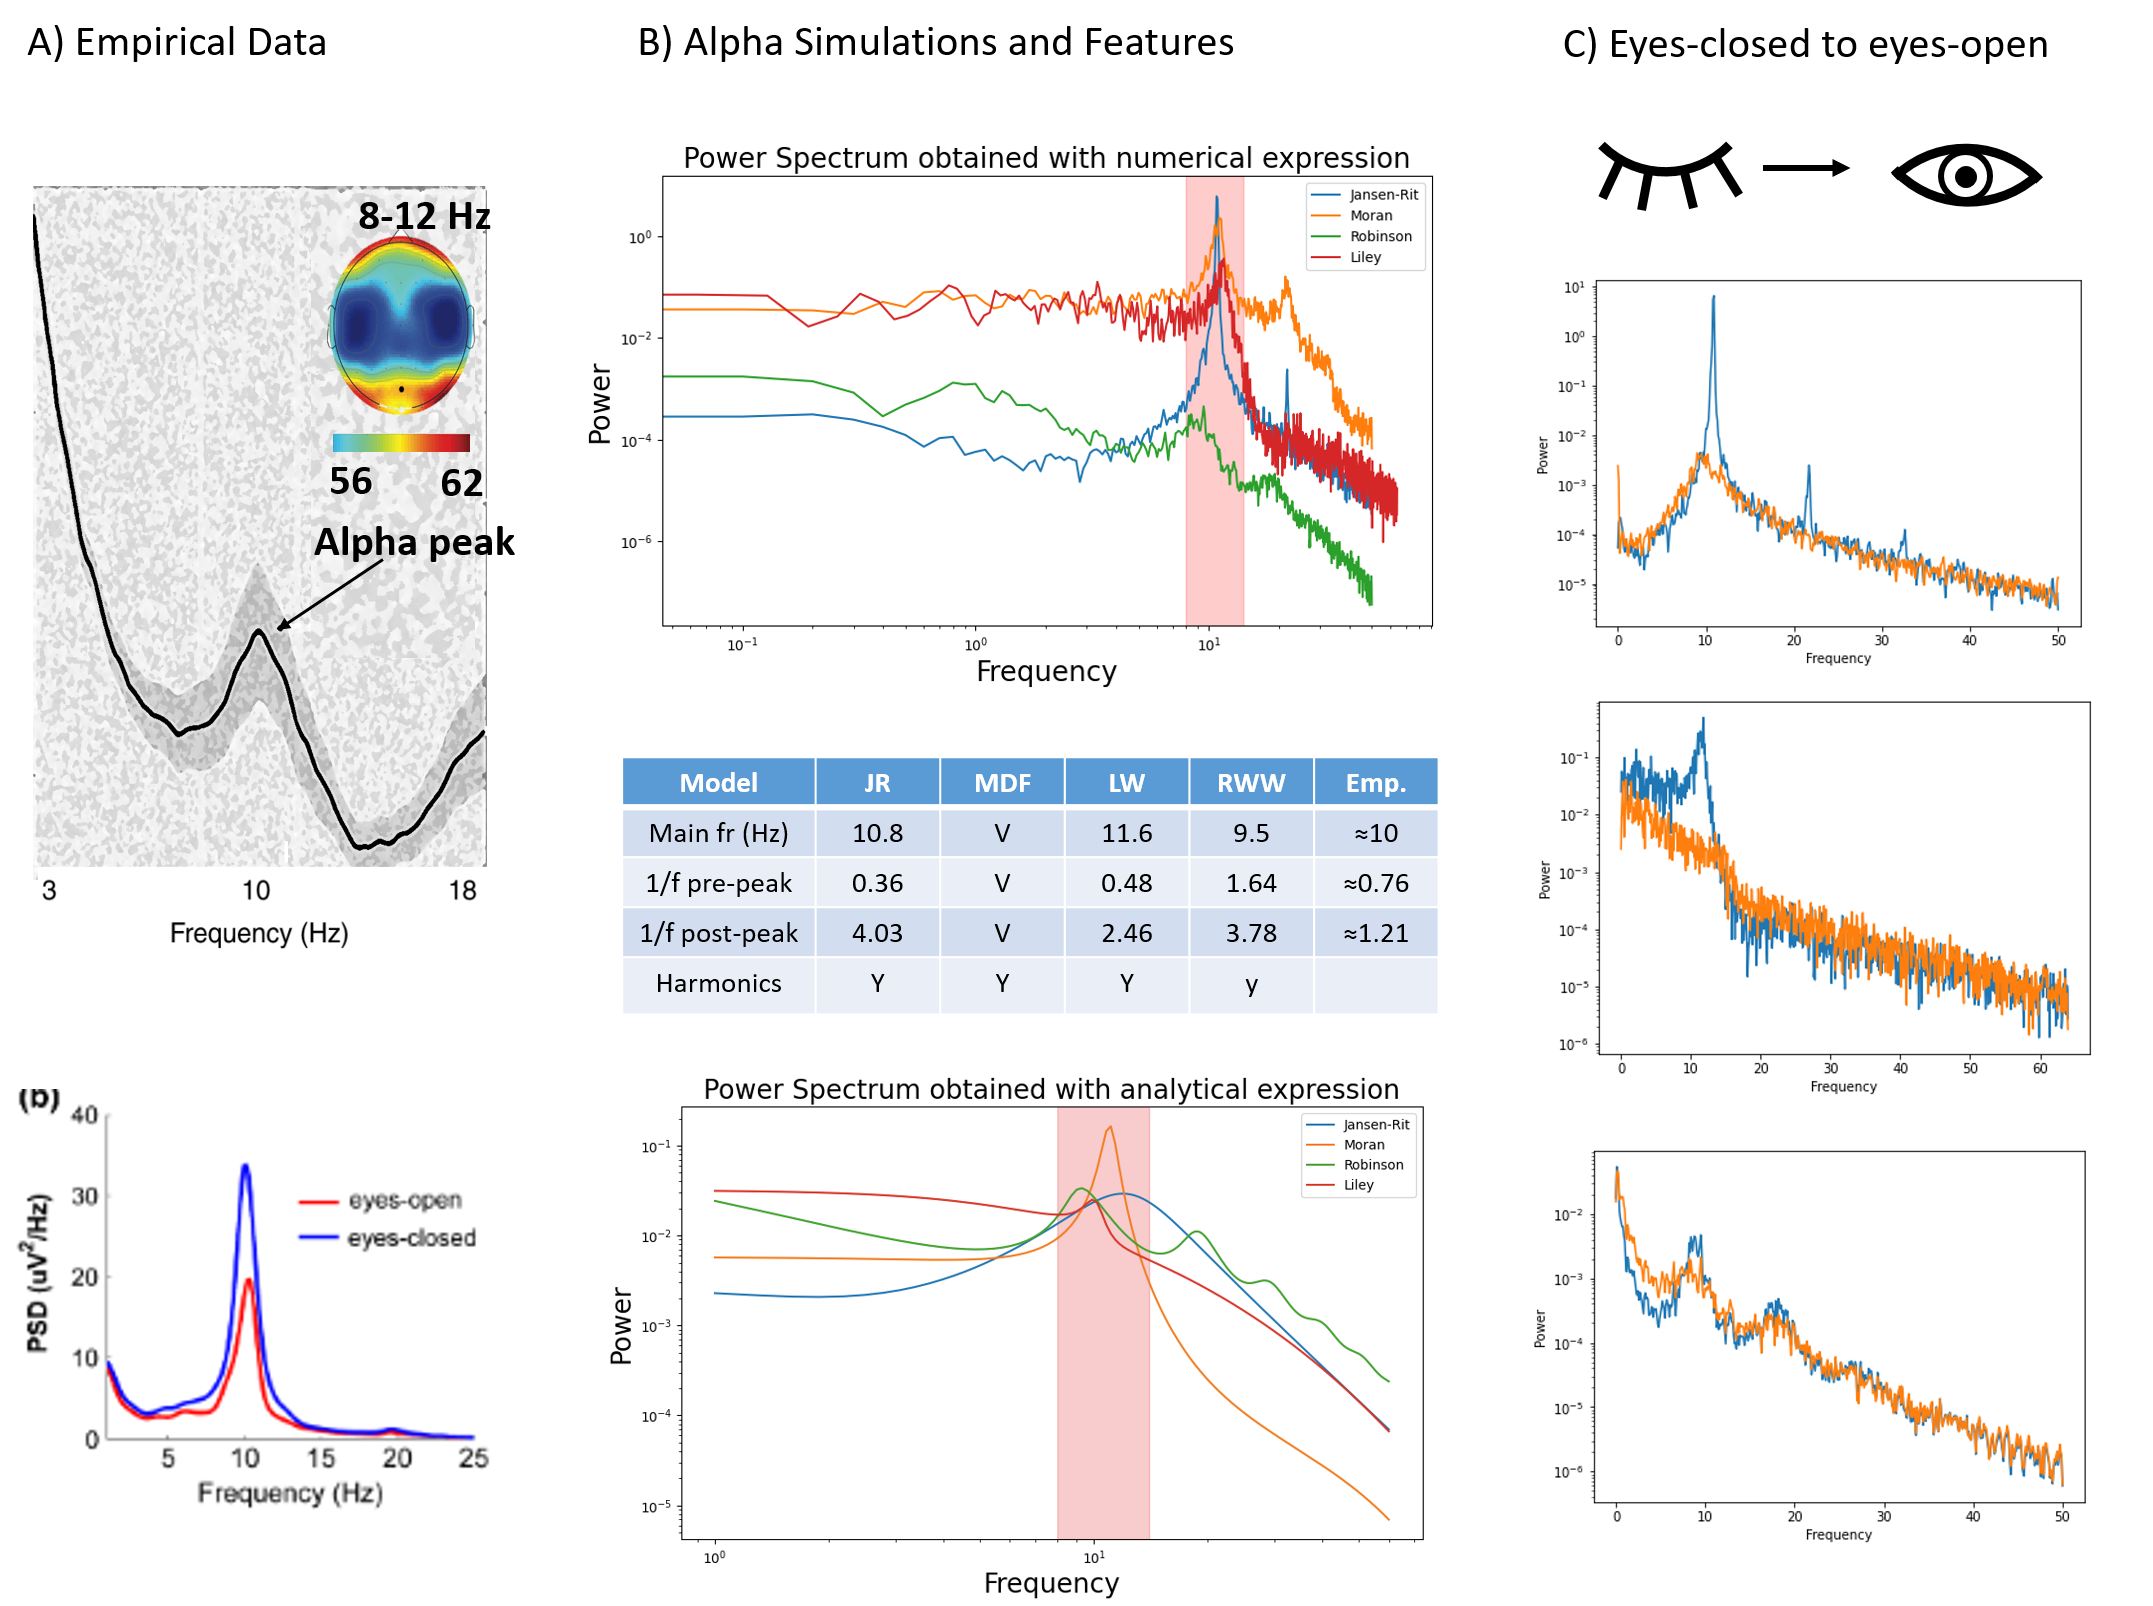
\includegraphics[scale=0.5]{Images/Alpha_all_results.png}
   % \caption*{\textbf{Figure 12.  \textit{Simulations results of each model to reproduce alpha oscillations with numerical (left) and analytical expression (right).}} All model generate alpha oscillations (peak in red zone (8-12Hz). Difference in shape, amplitude and 1/f components}
    %\label{fig:Alpha_results}
%\end{figure}
%TC:ignore
\begin{figure}[H]
    \hspace{-1cm}
    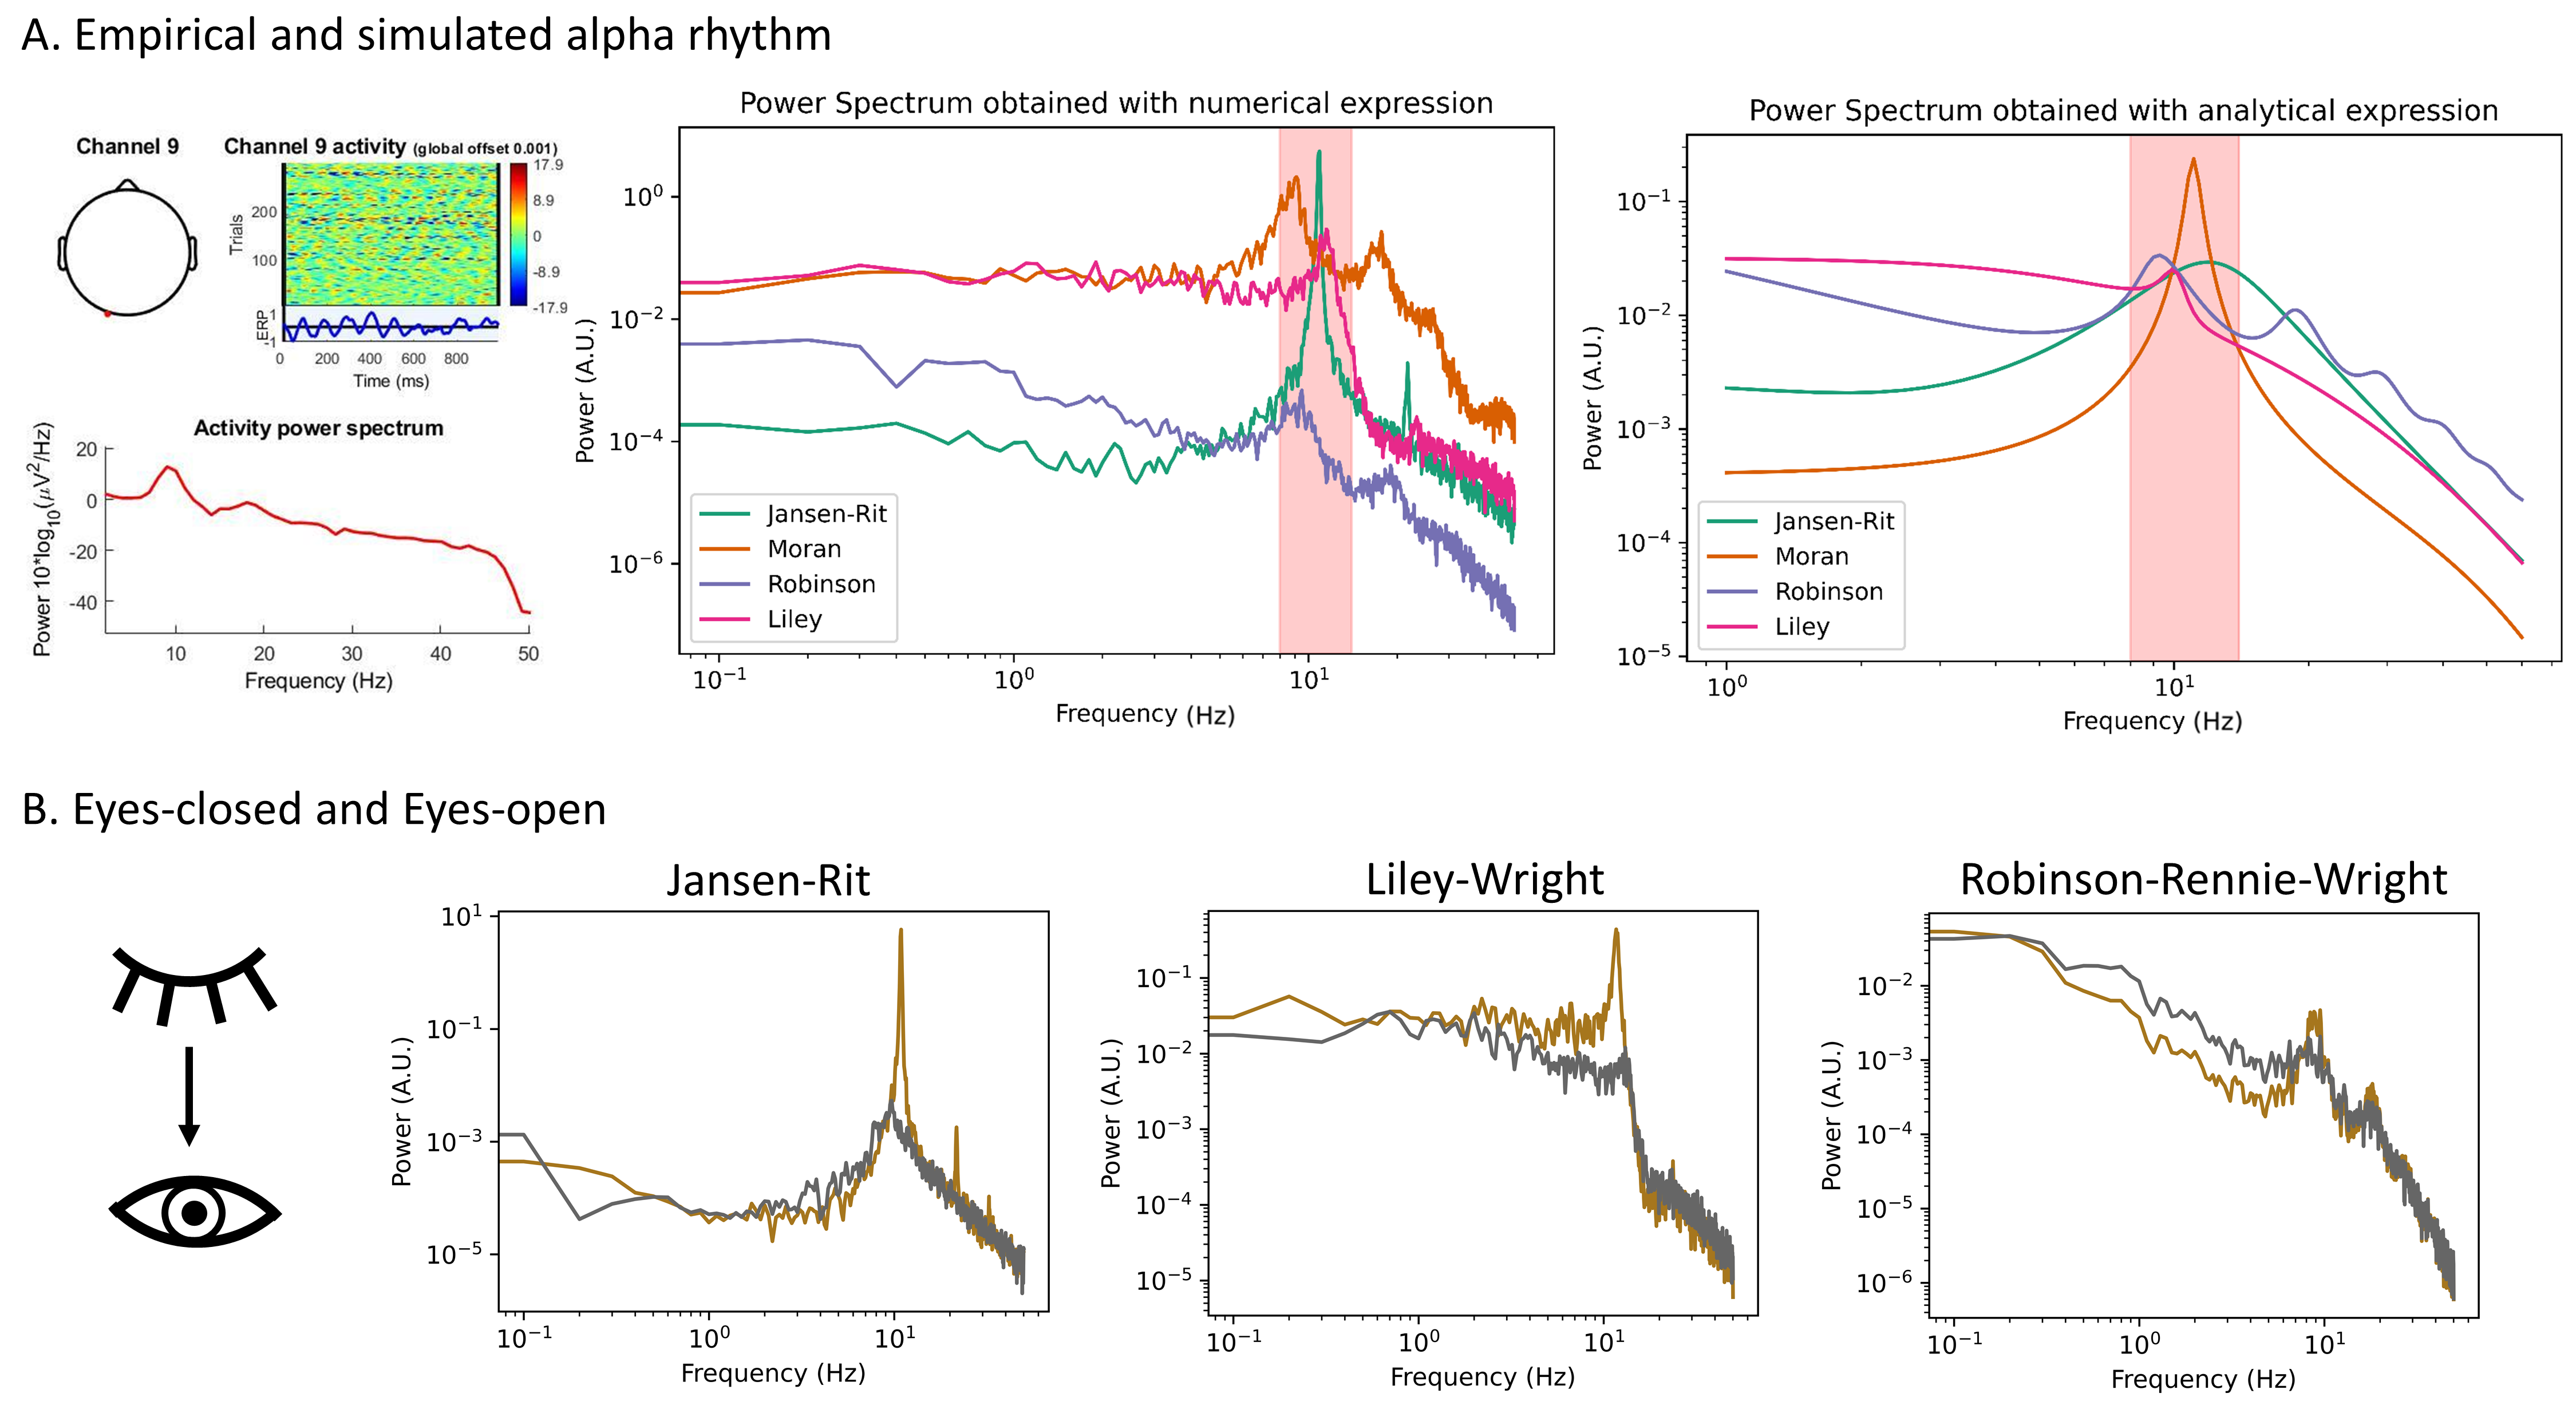
\includegraphics[scale=0.5]{Images/Figure_alpha_2.png}
    \caption*{\textbf{Figure 9.  \textit{Simulation results with standard parameter settings to generate characteristic resting state alpha oscillations features}} \textbf{A)} Power spectra with characteristic occipital alpha rhythm from empirical EEG time series (left), from numerical simulation results (middle), and from analytical simulations (right). The red zone in the simulated results corresponds to the alpha range. All models generate an alpha oscillation with variations in specific features (peak frequency, presence of harmonics, 1/f shape). \textbf{B)} Simulation results for EC and EO in JR, LW and RRW. The difference from EC to EO is an attenuation in the amplitude of the alpha rhythm.}
    \label{fig:Alpha_results}
\end{figure}
%TC:endignore

\begin{table}[h]  
\centering % centering table  
\begin{tabular}{l c c c c} % creating 10 columns  
\hline\hline   
Model & Main fr. & 1/f pre-peak & 1/f post-peak & Harmonics 
\\ 
\hline   
% Entering 1st row  
 JR & 10.8 & 0.39 & 4.04 & Y \\
% Entering 2nd row  
 MDF & 8.8 & 0.10 & 5.50 & Y \\
% Entering 3rd row  
LW & 11.6 & 0.48 & 2.46 & Y \\
% Entering 4th row
RRW & 9.5 & 1.64 & 3.78 & Y \\
\hline\hline % inserts single-line  
Empirical & $\approx$ 10 & 1.36 & 1.48 & Y\\
\hline
\end{tabular}  
 \caption*{\textbf{Table 1. \textit{Evaluating Model Performance against Empirical EEG Features}}  To assess the performance of each neural mass model, we estimated its characteristic features, such as the main frequency, slope, and presence of harmonics, and compared them against the corresponding empirical measures obtained from resting state EEG recordings. These features are known to be informative of the underlying neural dynamics that give rise to the EEG signal. By evaluating the agreement between the model-based estimates and the empirical approximations, we can determine the extent to which the model captures the essential aspects of brain activity during rest.}  
\end{table}  

% from source of We found that βhf values were generally highest and βlf lowest in occipital areas, implying less overall linearity in the scaling of the spectrum in these areas.
%TC:ignore
\subsubsection{Structure of parameter space}
%TC:endignore
Alpha oscillations are generated by non-unique parameter sets, and while there may be quantitative differences in parameter values between models, their qualitative behavior may be similar. In the next section, we explore alpha regime boundaries and the necessary conditions for producing a dominant frequency in the alpha range, as a function of rate constant and connectivity parameters. We also identify any other dynamical regimes that the model may present. Parameters with similar biological interpretations between the models are compared in order to provide a meaningful comparison.  
To ensure consistency, all other parameters are maintained in their standard resting state setting (Tables in Supplementary S.6).


\paragraph{Rate constant parameter space dynamics} ~\\
The JR, MDF and LW models exhibit distinct excitatory and inhibitory impulse responses that are modulated by rate constants ($\tau_{e}$ and $\tau_{i}$). These rate constants reflect collective passive dendritic cable delays and neurotransmitter kinetics associated with fast synaptic activity involving glutamatergic AMPA receptors and GABA receptors \citep{spiegler2012dynamics}. This synaptic filtering is assumed to take a different shape in excitatory than in inhibitory neural populations in most of the four models, with the exception of RRW - where the same rate constant is used for AMPA as for GABA receptors. Previous studies have demonstrated that the manipulation of these rate constants can significantly impact the dominant frequency of oscillations \citep{david2003neural, gast2019pyrates}. In our investigation, we aim to determine whether similar patterns of frequency changes can be observed across the parameter space for all three models. \\
%TC:ignore
\begin{figure}[H]
    \centering
    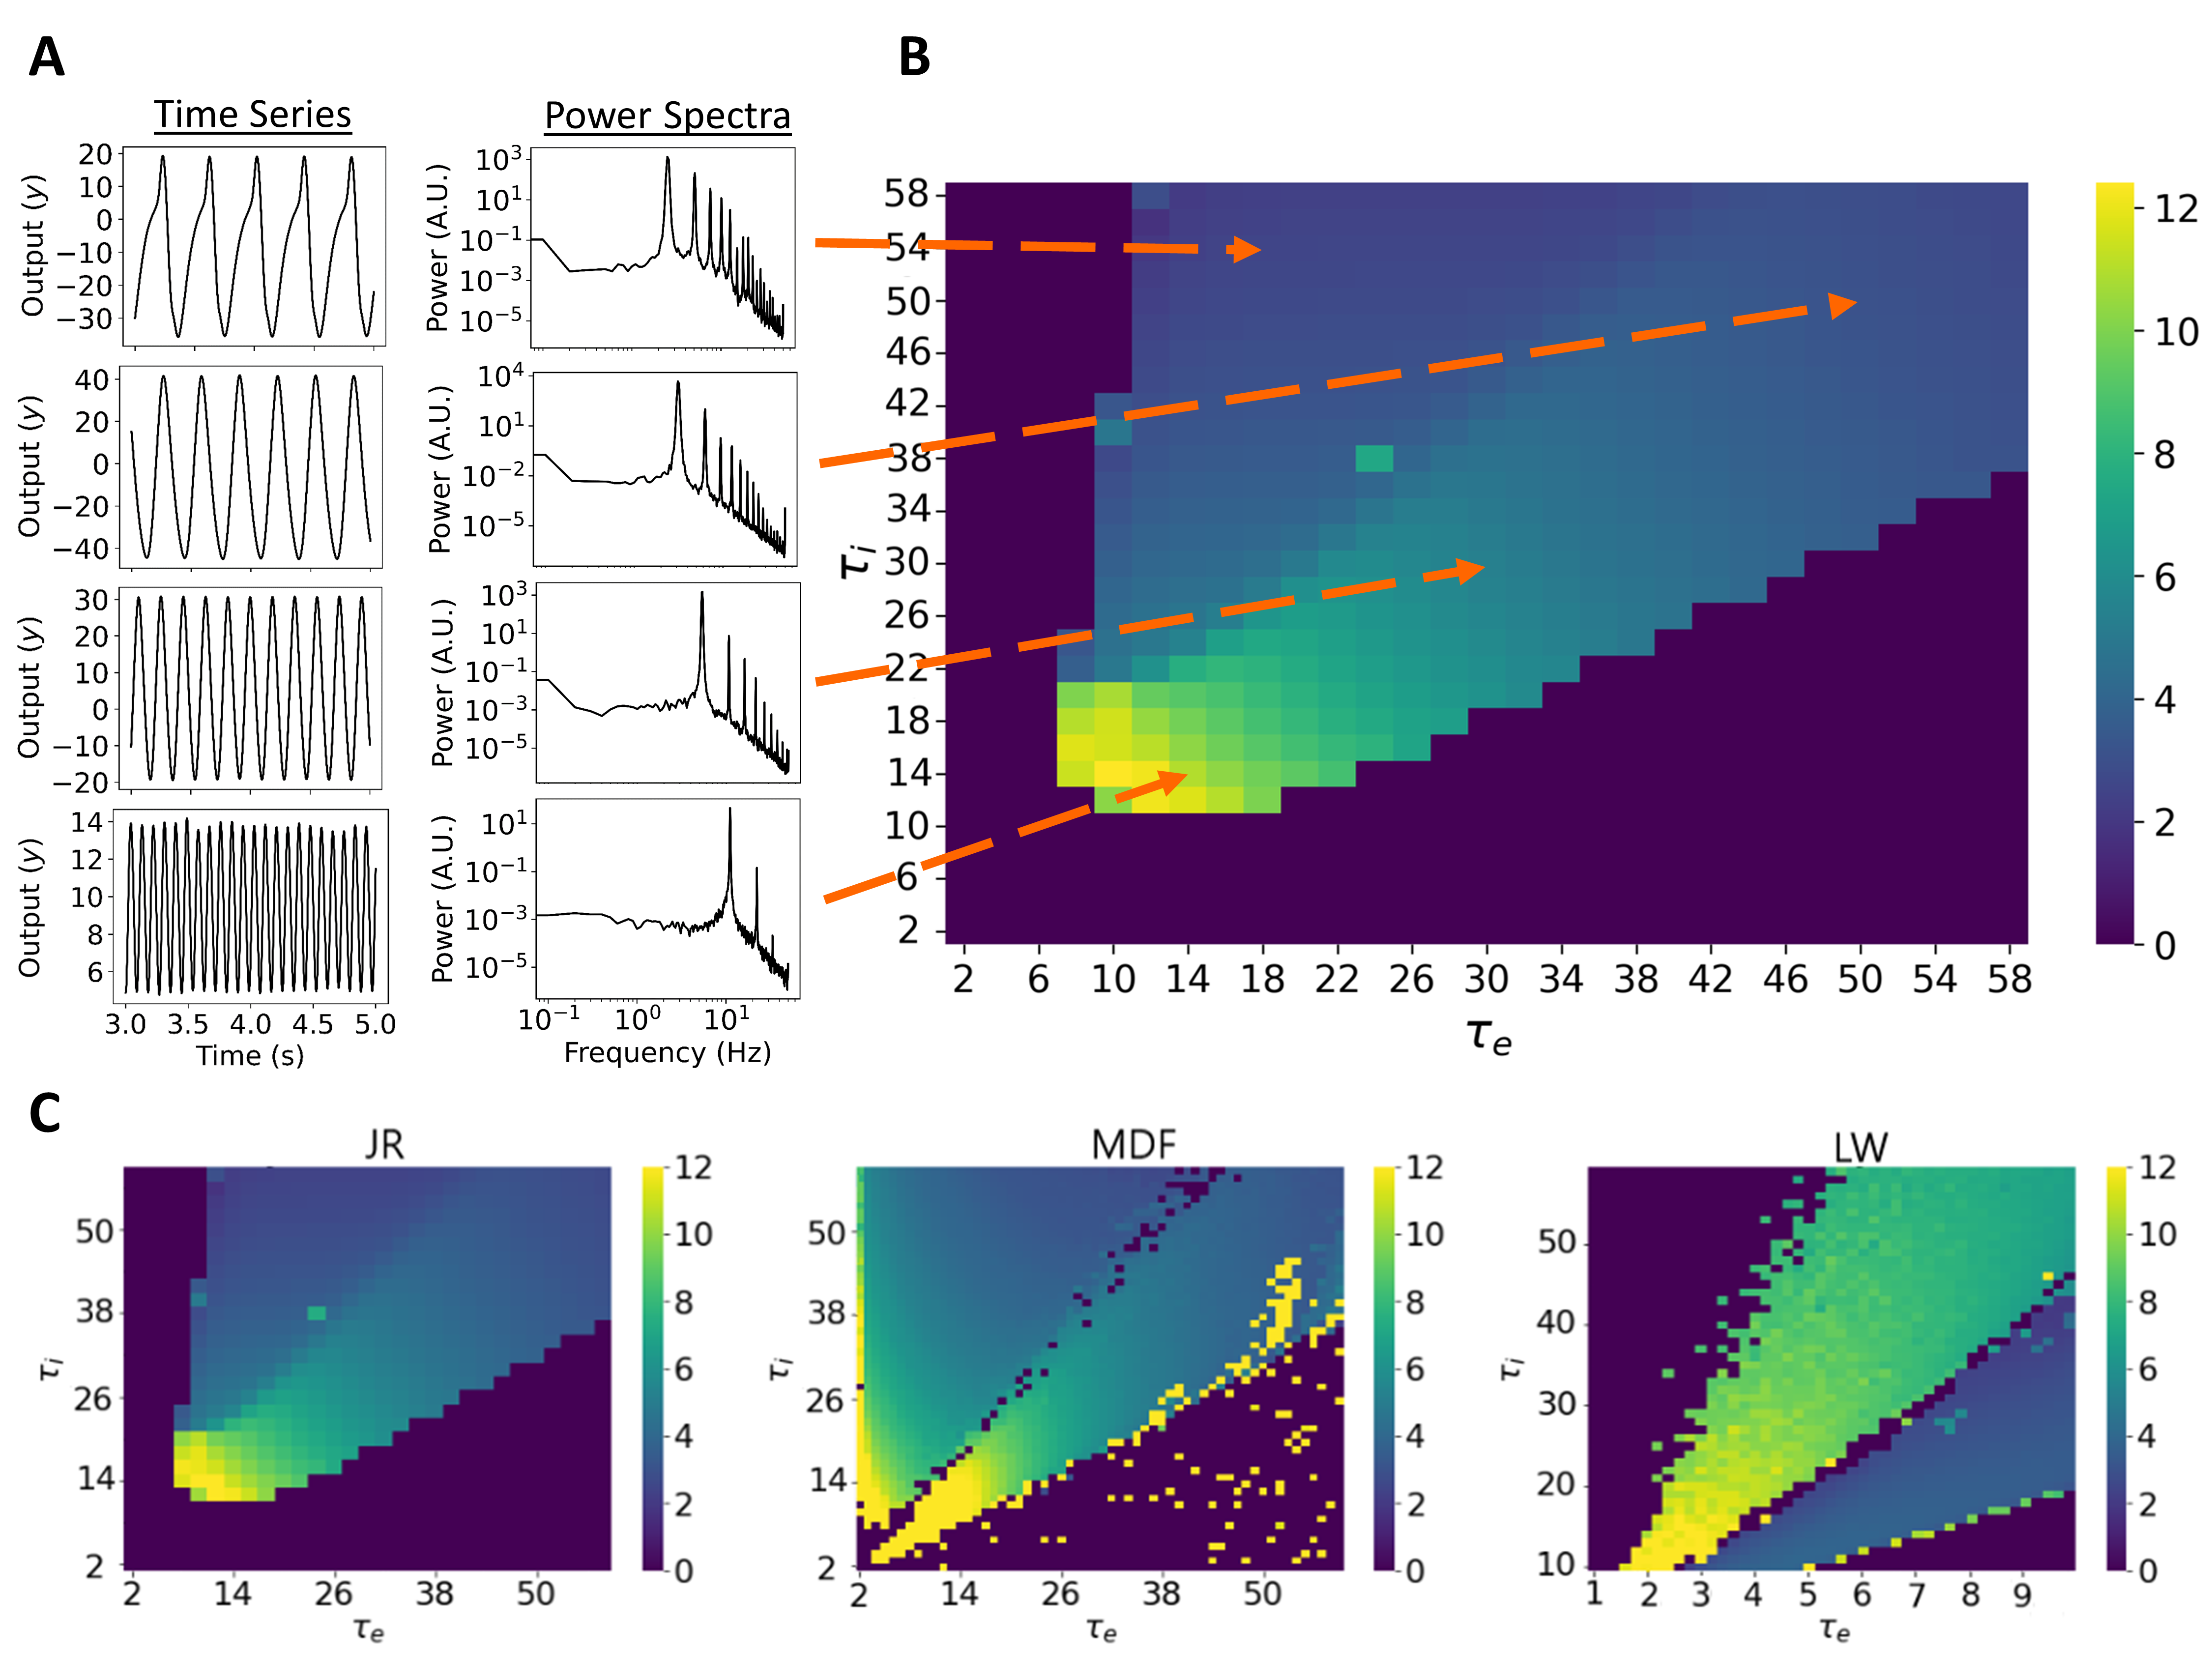
\includegraphics[scale=0.45]{Images/Rate_constant_4.png}
    %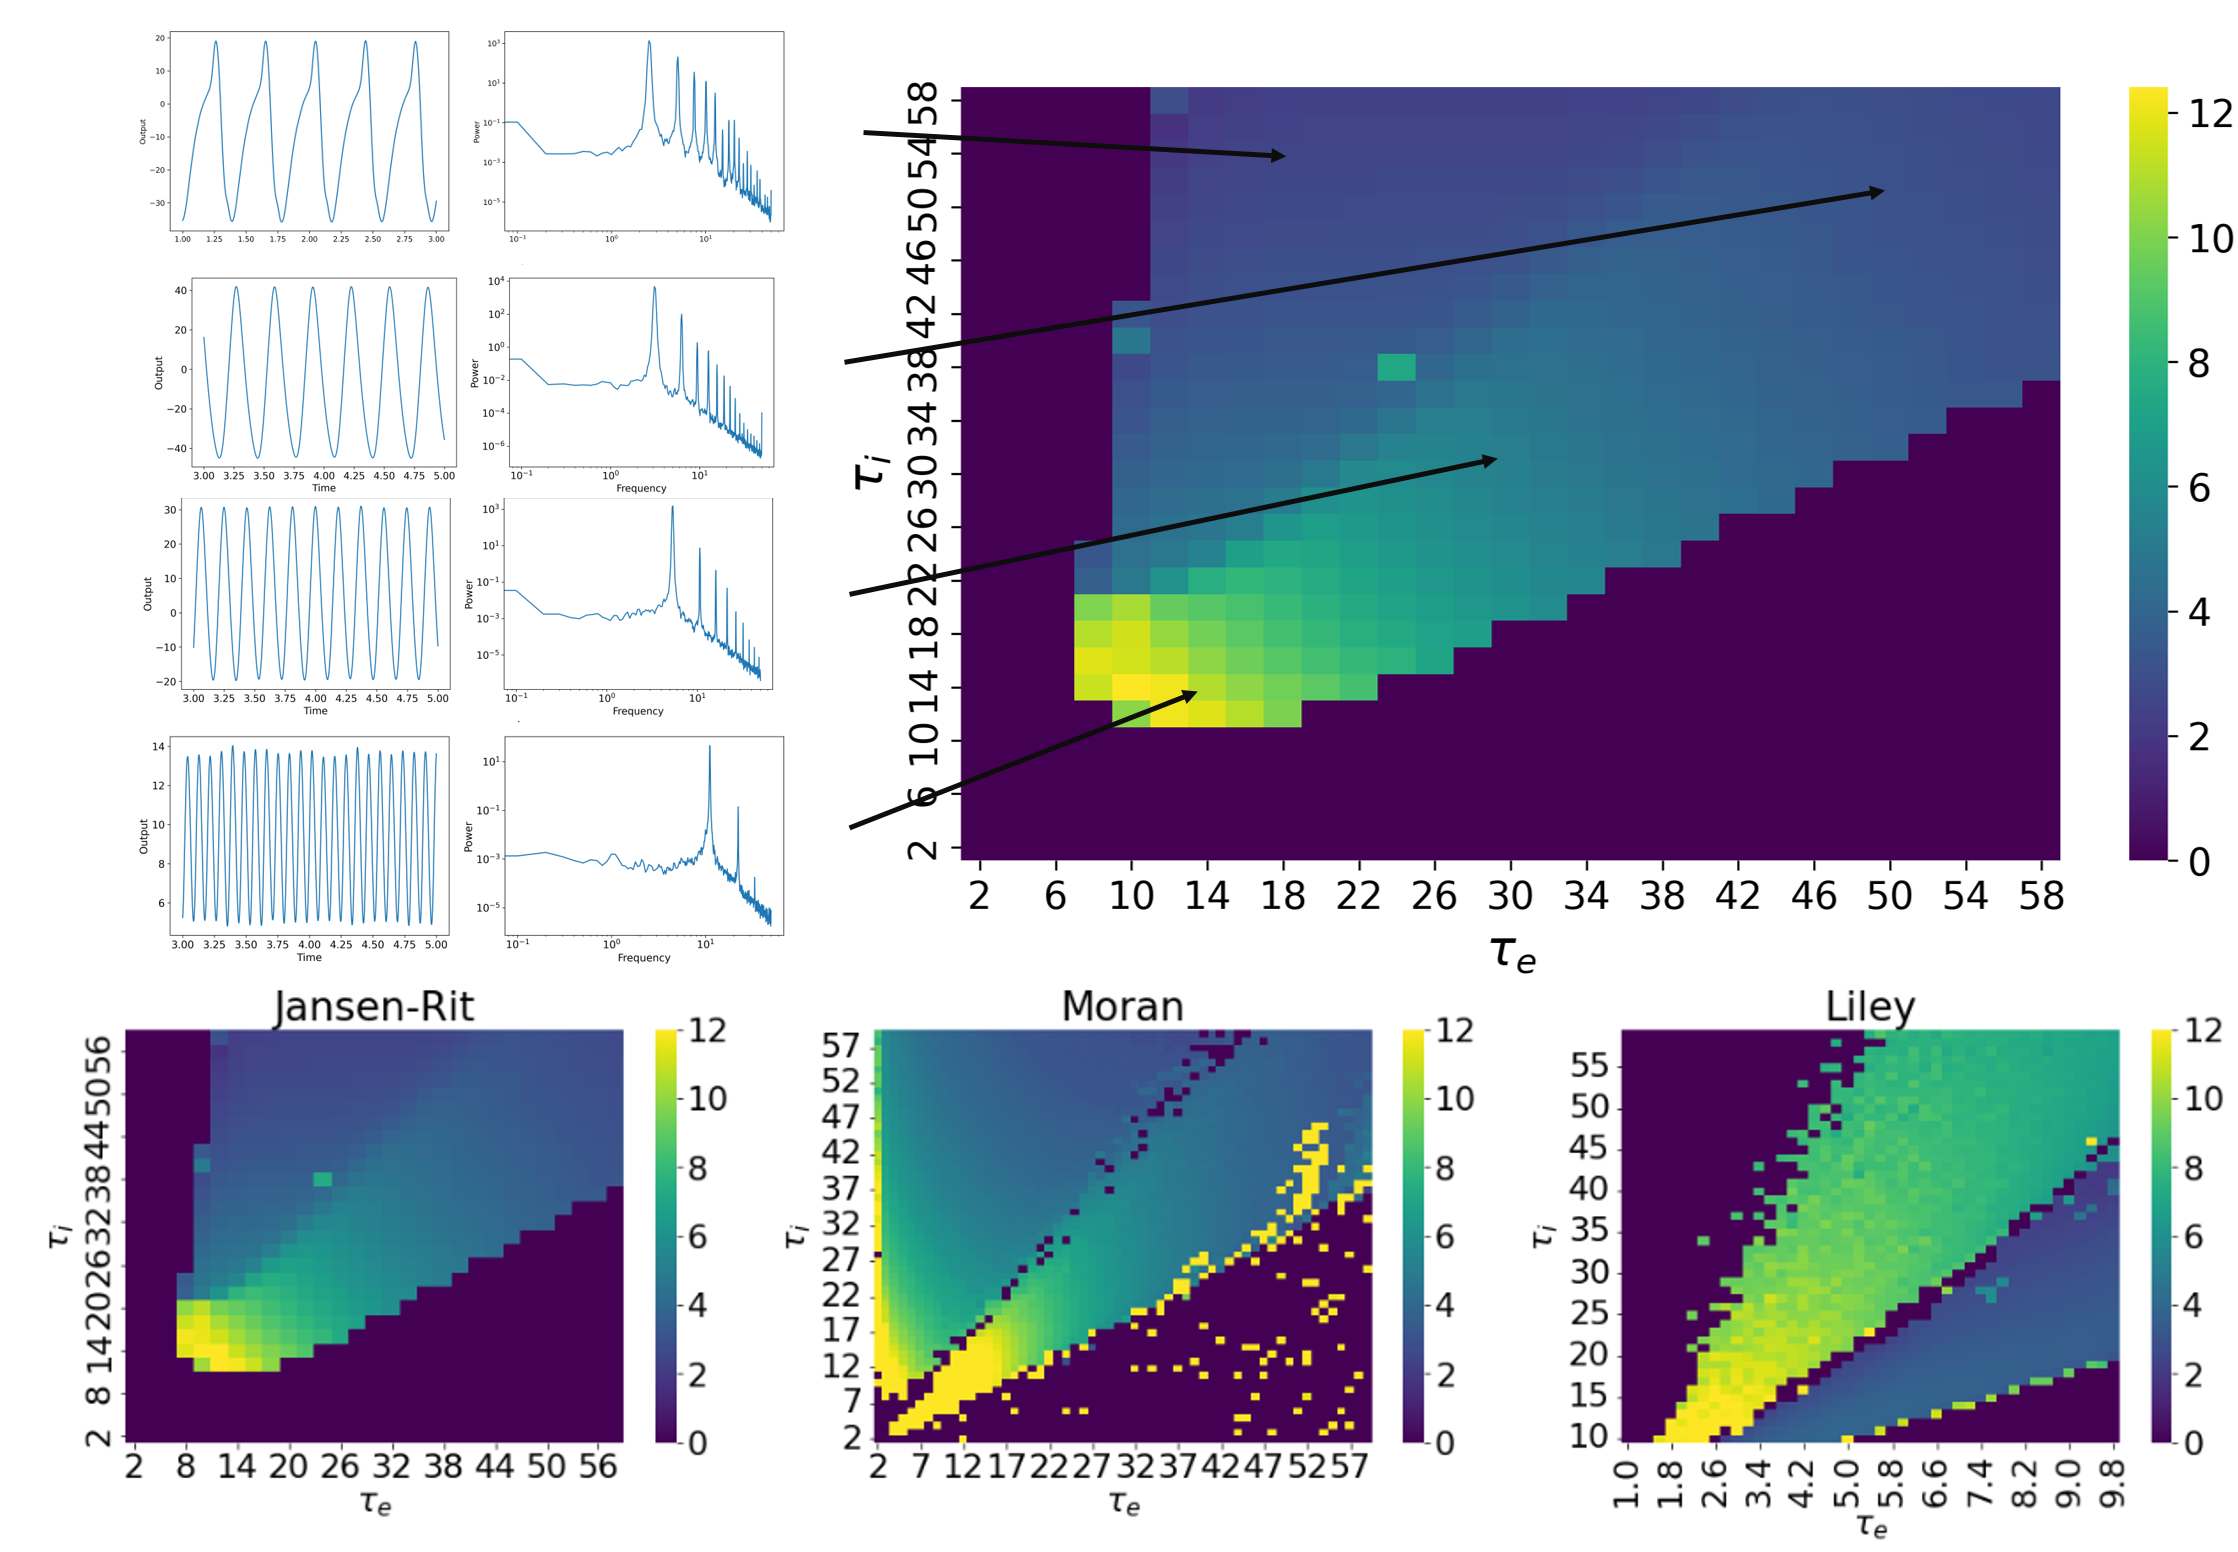
\includegraphics[scale=0.48]{Images/Rate_constant_2.png}
    \caption*{\textbf{Figure 10.  \textit{Effect of rate constants on dominant frequency of oscillation for the JR, MDF, and LW models.}} 
    \textbf{A)} Example time series and power spectra of a set of specific rate constant values to show the slowing in frequency as the values of the excitatory and inhibitory rate constant increase. \textbf{B)} Heatmap presenting the dominant frequency of oscillation as a function of the rate constants of the JR model. \textbf{C)} Three heatmaps for the JR, MDF and LW with the dominant frequency of osicllation as a function of the rate constants. For JR and MDF $\tau_{e}$ and $\tau_{i}$ are varied from 2ms to 60ms. For LW, $\tau_{e}$ changes from 1.72ms to 5ms, and $\tau_{i}$ from 10 to 50ms to generate oscillatory behavior.}
    \label{fig:tau_param_sweep}
\end{figure}
%TC:endignore
Across all models, a consistent trend is observed where the predominant rhythmic frequency decreases with an increase in both rate constants, aligning with previous analyses \citep{david2003neural}. For the LW model, the range of values for $\tau_e$ and $\tau_i$ differs due to the system's tendency to diverge if $\tau_e$ becomes excessively high compared to $\tau_i$. Due to this, in Fig. 10 we constrain the possible range of values to 1-10 ms for $\tau_e$ and 10-60 ms for $\tau_i$.
% this argument needs to be developed: An explanation for the difference is the presence of an additional neural population in JR and MDF which compensates. Furthermore, this might reflect a more accurate biological model as not any values can be used to represent the rate constants. \\
With a uniform external input, the JR model has a peak oscillatory frequency of 12.4 Hz, falling within the high alpha / low beta range. MDF can elicit higher beta oscillations with a normal noise input when rate constant are both small. This suggests that the inclusion of self-inhibitory connections in MDF contributes to generating higher frequency oscillations. Notably, both JR and MDF exhibit a phenomenon known as a `hypersignal' \citep{david2003neural} when $\tau_i$ is considerably higher than $\tau_e$, which is typically associated with lower frequency oscillations. In such cases, the time series does not produce an exact sinusoidal oscillation (Fig. 10). Conversely, if $\tau_e$ becomes too high compared to $\tau_i$, neither model shows oscillatory patterns. This means that a balance needs to be kept in order to maintain a periodic behavior, which can be achieved by keeping the product of $H_{e,i}$ and $\tau_{e,i}$ constant by appropriately adjusting $H_e$ and $H_i$ as $\tau_e$ and $\tau_i$ is modified \citep{david2003neural}. 

In the LW model, equivalent hypersignal behavior is observed when $\tau_e$ is excessively high compared to $\tau_i$, while in the opposite case of $\tau_i$ higher than $\tau_e$ no oscillatory activity is seen. Furthermore, as shown in Fig. 10, this hypersignal activity occurs above the alpha regime in $\tau_e$ vs $\tau_i$ space for JR and MDF, and below the alpha regime for LW (Fig. 10). What these observations suggest is that the central alpha oscillatory regime in JR and MDF operates in a manner that is intrinsically different to the alpha regime in LW - a question we revisit through the lens of linear stability analyses below. 

As expected, modifying the shape of the synaptic filtering through the rate constants has an influence on the rhythmic behavior of the system. Increasing both rate constants simultaneously leads to a decrease in the frequency of oscillation since longer delays are then introduced. For example, if a disease affects the propagation of action potentials, it could lead to a decrease in the dominant frequency of oscillation.
In the RRW model, $\tau_{e}$ and $\tau_{i}$ are assumed to be equal, considering that the difference in rise time between AMPA and GABA-A is negligible and, therefore, the synaptic filtering is the same between excitatory and inhibitory neurons. This assumption can be questioned as changes in rate constants in the other models have been shown to affect the central frequency. 

% Spiegler 2012 for JR: Second, the analysis revealed that the intrinsic temporal ratio β between the inhibitory and excitatory dendritic time constants τi and τe (not their absolute values) determines whether no oscillations, only onetype of oscillation (harmonic or anharmonic) or both types are possible (Fig. 5.4; this confirms the findings of David and Friston [48]). Regarding the system Eqs. (4.1) to (4.7), it is obvious that the dendritic time constants are related to each other by their scaling or respectively the intrinsic temporal ratio β = τe/τi. Hence, the system behavior qualitatively depends only on the intrinsic temporal ratio β and on the extrinsic inputs on both types of interneurons (i. e., EINs and IINs). More specifically, this analysis revealed that for maintaining an oscillatory regime, it is essential to keep the ratio β ≤ 5 (see Fig. 5.6).


\paragraph{Connection Strength} ~\\
The strength of connections between neural populations plays a role in facilitating communication, and thus when the strength of these connections is appropriately balanced, it enables coordinated neural activity, leading to the generation of brain rhythms. Even though on the face of it the neural populations included in the four models differ quite considerably, they all exhibit at least one common element - a principal excitatory-inhibitory ($E - I$) loop. The ratio of synaptic weights within that loop relates closely to the concept of `E/I balance', a widely studied physiological phenomenon that has garnered significant attention in neuroscience in recent years \citep{meisel2017decline, zhou2018synaptic, sohal2019excitation, murray2014linking}. We explored the impact of connectivity parameters on the dominant frequency of oscillation. To maintain conciseness, we exclude the connectivity parameter spaces of MDF in this section, since the patterns observed are very similar between JR and MDF, with the distinction that MDF tends to generate higher frequencies of oscillation for the same set of parameter values. A comprehensive summary of the comparison between JR and MDF can be found in Supplementary S.2.
%The comparison between JR and MDF is summarized in the Appendix B. \\

%TC:ignore
\begin{figure}[H]
    \centering
    %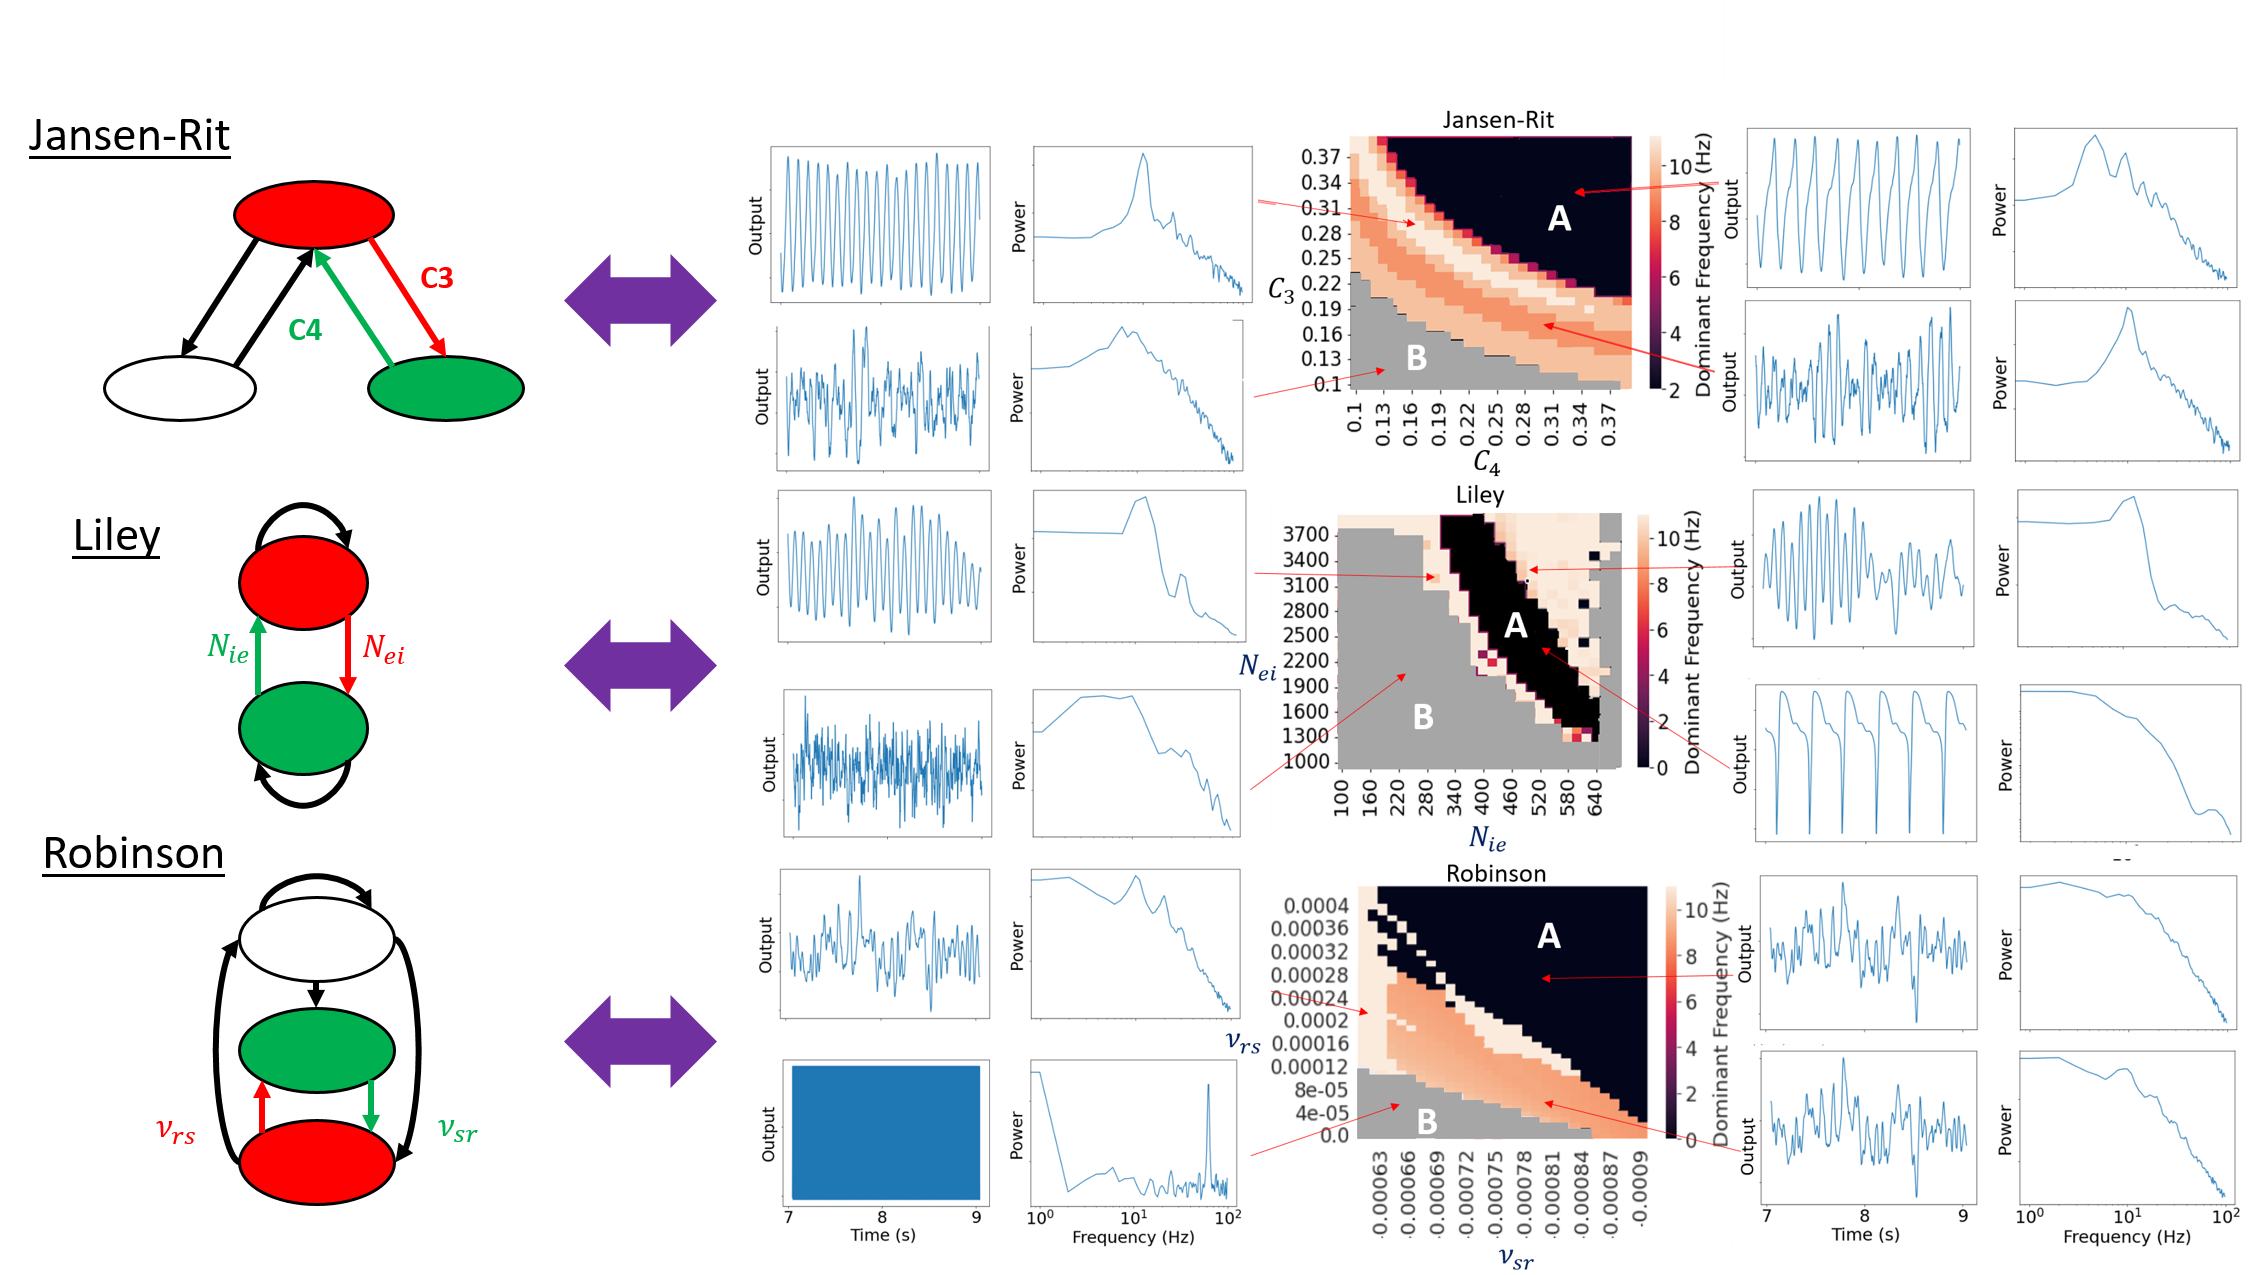
\includegraphics[scale=0.49]{Images/Connectivity_final.png}
    %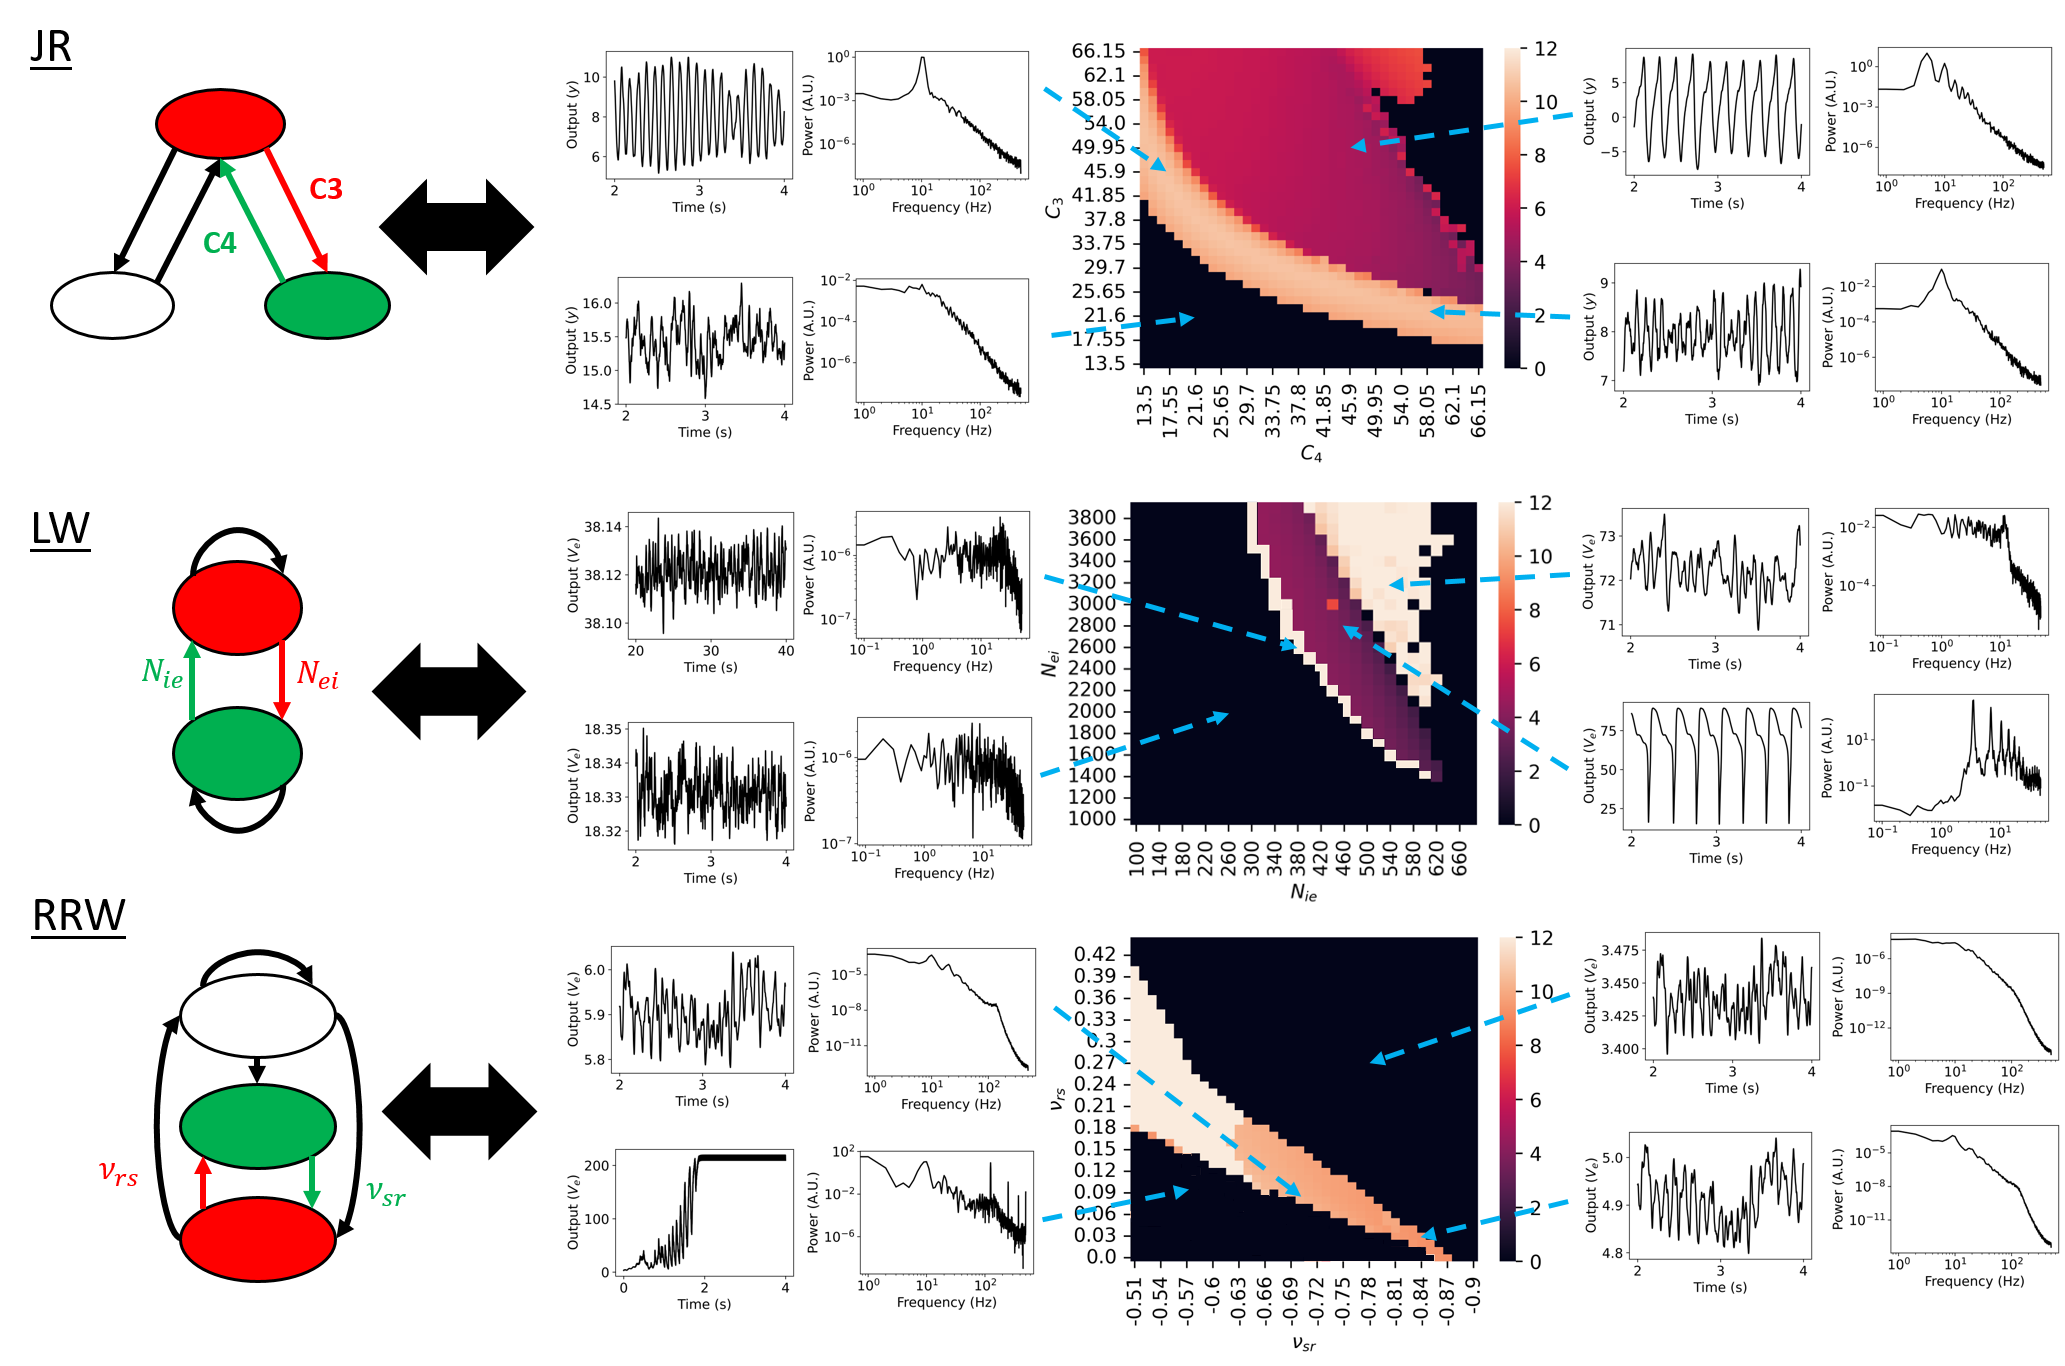
\includegraphics[width=\linewidth]{Images/Connectivity_3.png}
    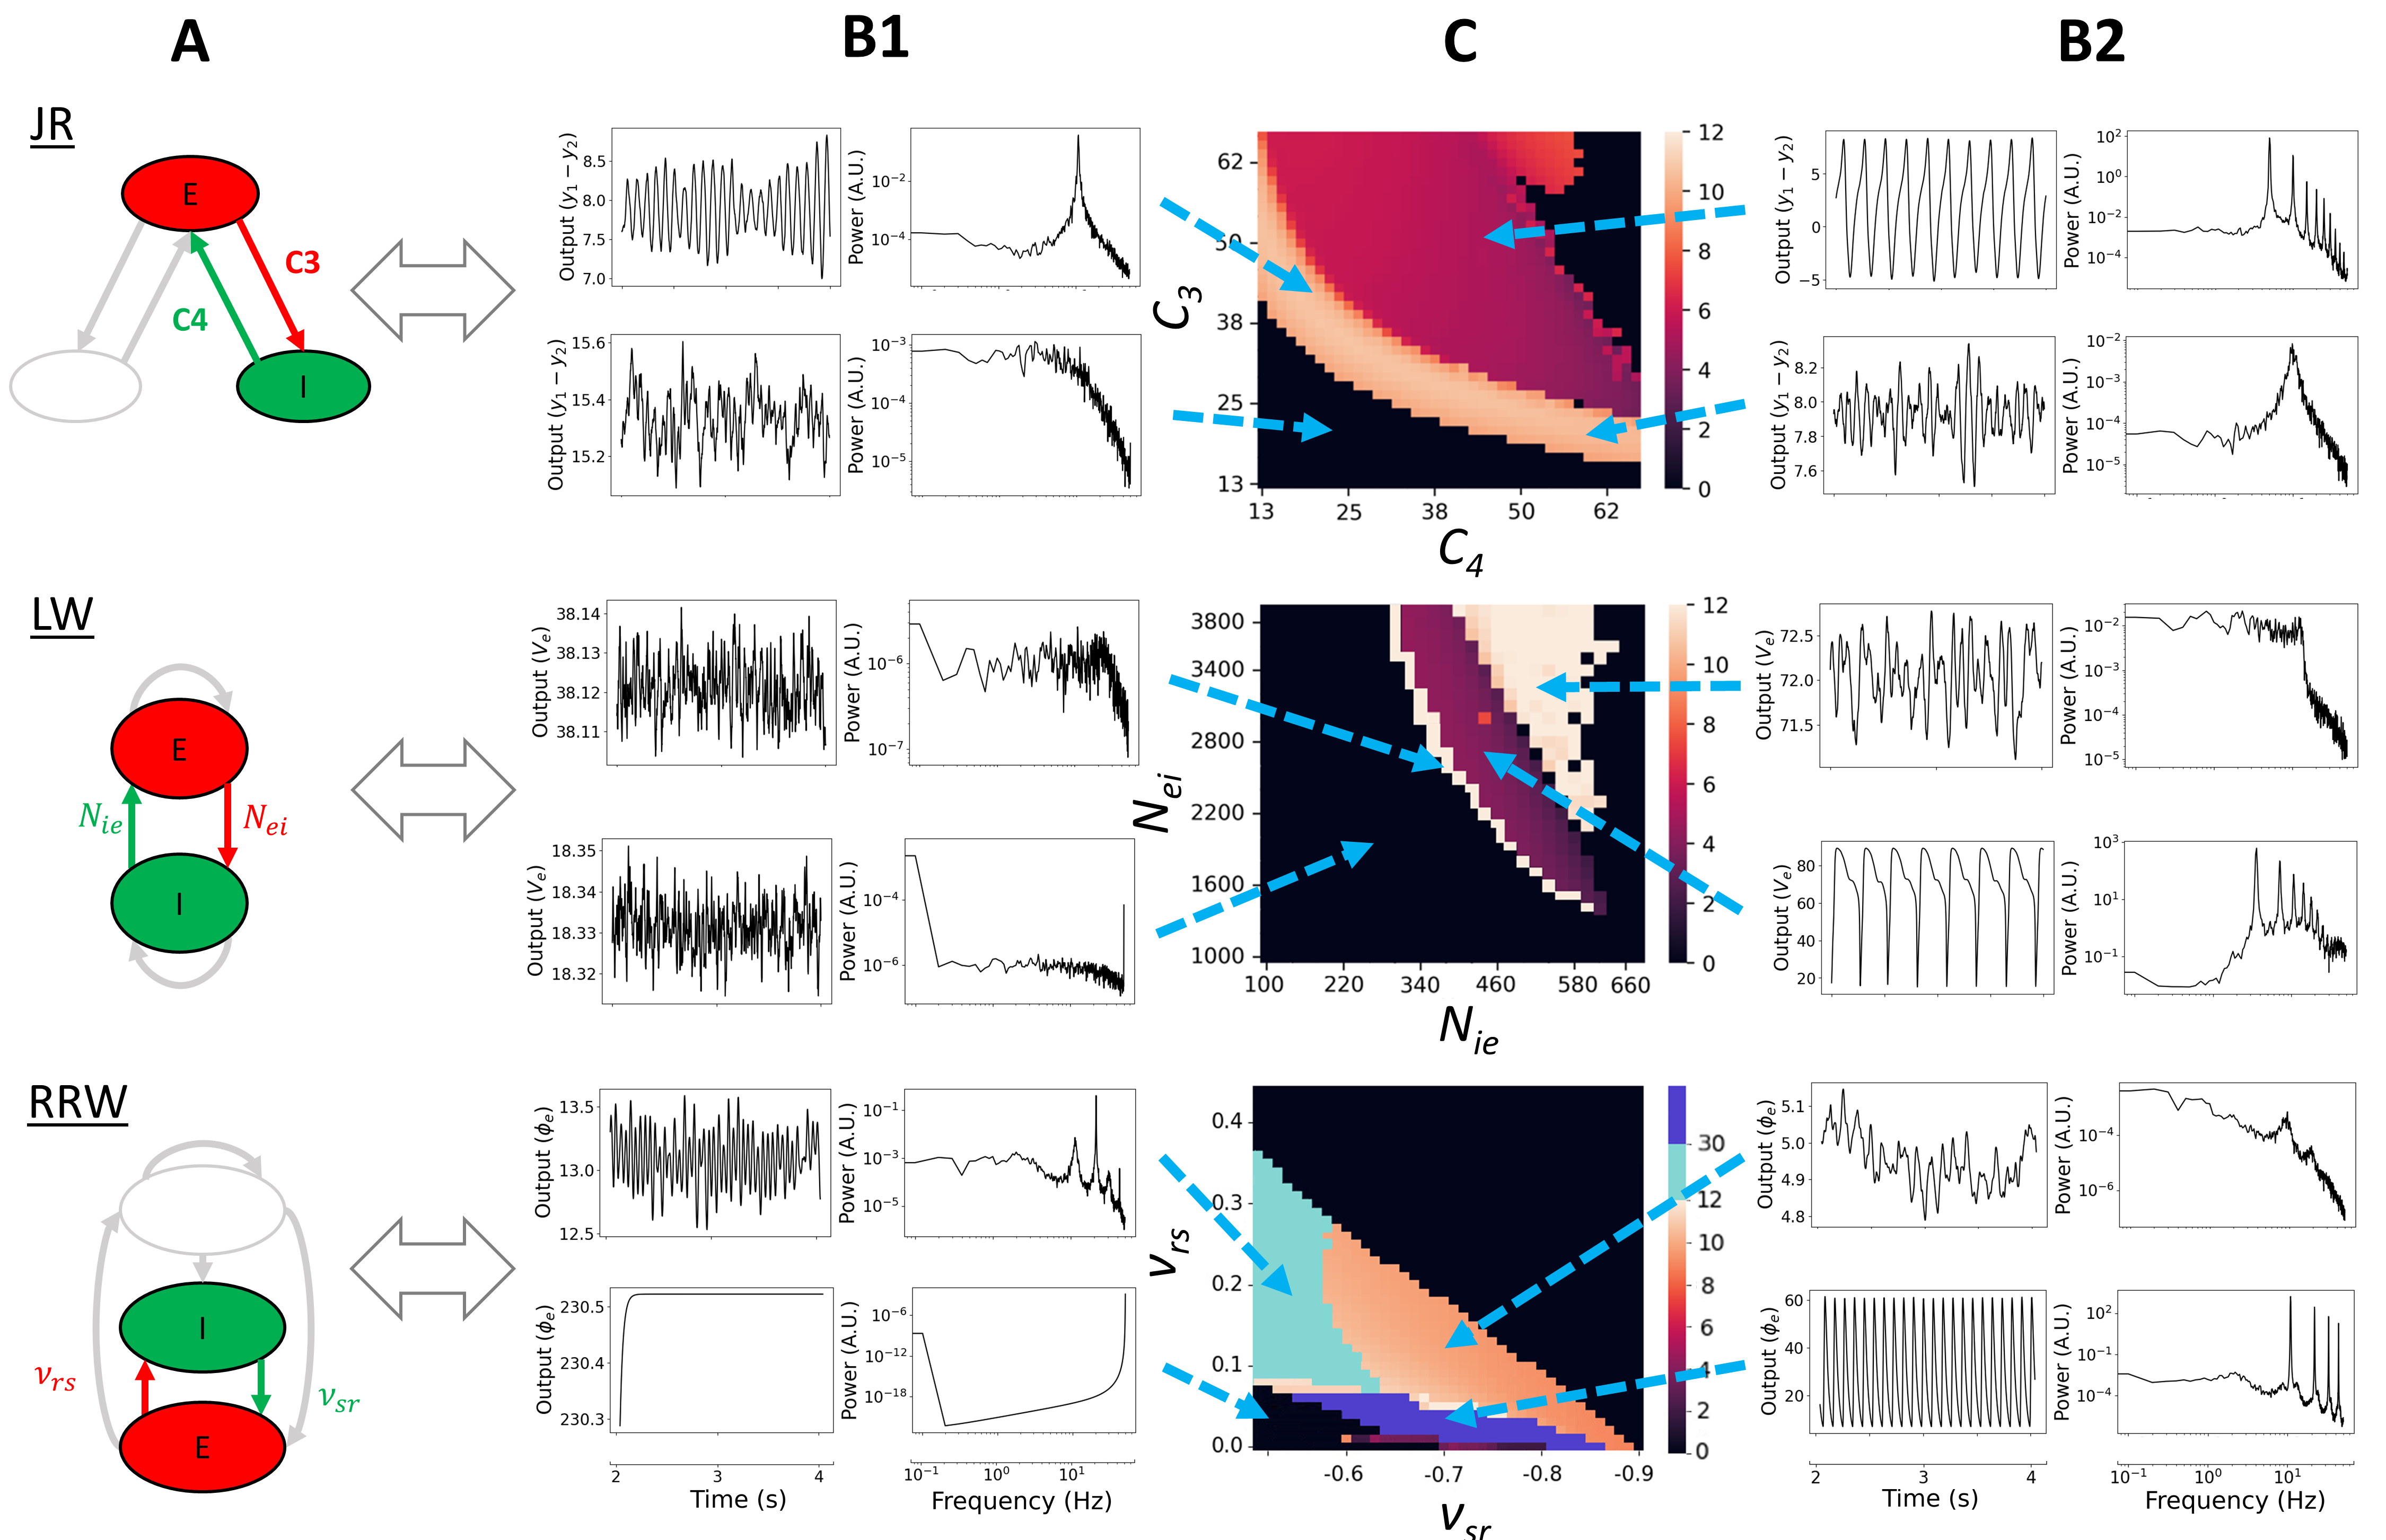
\includegraphics[width=\linewidth]{Images/Connectivity_5.png}
    \caption*{\textbf{Figure 11.  \textit{Frequency of oscillation parameter spaces as a function of E-I connectivities}} \textbf{A)} Schematic of the models with their principal E-I loop highlighted. These are the parameters that are going to be varied. \textbf{B1 and B2)} Time series and corresponding power spectra for specific combinations of E-I, showing different dynamics. \textbf{C)} Heatmaps presenting the dominant frequency of oscillation as a function of E-I connectivity. The dark region presents non-oscillatory or non-physiological time series. JR and LW have a clearly defined regime of lower frequency of oscillations being generated (purple and red region), whereas RRW quickly tends to produce signals of lower amplitude, or higher frequency of oscillations. In RRW, the dark blue regime indicates that the system is still oscillating but at a higher amplitude and higher frequency as the system is starting to explode. In the light blue regime, the dominant frequency of oscillation is in the beta regime. In the three models, white or orange areas correspond to alpha or higher oscillations.} \label{fig:All_EI_Together}
\end{figure}
%TC:endignore
JR's E-I interaction is represented by the connectivity strength between pyramidal cells and inhibitory interneurons. Since the LW model is only composed of one excitatory and one inhibitory neural population, the parameters of interest are the two synaptic weights connecting the two populations. Finally, for RRW, the reticular nucleus inhibits the relay nuclei and is considered the inhibitory population of the model. In this context, we consider the relay nuclei as having a central role and can be compared to the pyramidal cells in the JR model, as they are connected to all other populations. The excitatory-inhibitory interaction explored is then within the thalamus between the relay nuclei and the reticular nucleus. It should be noted that this interaction is not an isolated loop, because it is embedded within the larger cortex-reticular nucleus-relay nuclei loop, and so is also affected by the activity from the cortex. However, for simplicity, our focus is on the E-I interaction between the two thalamic populations.

After exploring various parameter ranges, we identified specific values that produced distinct behaviors for each model, and focused on these dynamic regimes. Results of these analyses are shown in Fig. 11. As can be seen in the heatmaps, we observe an inverse diagonal relationship between E-I connectivity and the parameter regime giving rise to alpha frequency oscillations in all three models. This illustrates the fact that it is the total amount of E-I connectivity, or the total E-I gain, that defines the presence of alpha rhythm in these models.

A second common feature across all three models is that if the excitatory or the inhibitory connectivity is too low, non-physiological results are obtained. These include time series with either very low amplitude or very high frequency (dark region in Fig. 11 panel D), highlighting the importance of the interaction between these two populations for the generation of rich neural dynamics. 

The relationship between $C_{3}$ ($P \rightarrow I$) and $C_{4}$ ($I \rightarrow P$) in JR in order to generate alpha oscillations correspond to an exponentially decaying function. A similar correspondence is observed in the LW model, although with a narrower range of possibilities due to model constraints. Furthermore, LW presents a steeper slope, indicating a stronger effect on the dynamical regime of the input from GABA interneurons ($N_{ie}$) on the frequency than the input to GABA interneurons ($N_{ei}$).
Both the JR and LW models generate lower frequency oscillations, corresponding to the hypersignal regime, as observed in the analysis of rate constant parameter space (purple color in the JR and LW heatmaps in Fig. 11 C, rows 1 and 2). In the LW model, if the connectivities are increased beyond this regime, predominantly alpha-frequency activity is generated (triangular white zone above the purple region), which corresponds to the dynamics observed with standard connectivity parameter values. To better understand this difference, a local stability analysis was performed to define the fixed points of the JR and LW models, and expand on their dynamical characteristics (Fig. 12). In the case of JR, the colored alpha regime presents unstable fixed points that continue into the hypersignal regime. These oscillations are due to an Andronov-Hopf bifurcation, wherein the system enters a limit cycle that changes shape over time (Fig. 12, 1a and 1b). In LW, an Andronov-Hopf bifurcation also occurs, explaining the hypersignal and some higher frequencies on the left hand side of the lower frequency region (Fig. 12, 3a and 3b), including alpha. However, the alpha regime in LW generated with standard parameter values lies within the space of stable fixed points (Fig. 12, star in 3b), which corresponds to the triangular white regime in the LW heatmap (Fig. 11, C LW). This implies a separate emergent mechanism of alpha rhythm in LW that is distinct from the emergence of a limit cycle that is seen in JR. The generated alpha in this setting is noise-driven, since without noise the system becomes a damped oscillator (due to its having complex eigenvalues with negative real part), and eventually reaches the fixed point (Fig. 12, 4a and 4b). The noise fluctuations repeatedly push the system away from its fixed point at the frequency of alpha, but it tends to stay around that stable point instead of reaching a self-sustaining limit cycle oscillation. 
%This finding is consistent with the observations of previous authors that the LW model can produce different types of alpha rhythms that are not continuous in parameter space \citep{liley2014neural}. %check where in the source exactly. 
The stability analysis presented here corroborates the idea that the standard alpha rhythms generated by the LW and JR models constitute two mechanisms that are both physiologically and mathematically distinct. This is consistent with the rate constant and connectivity parameter space results as in the rate constant result, we could identify the hypersignal regime above the alpha regime for JR but below for LW, which is also seen in the connectivity parameter space result.

We also conducted an investigation into the effect of low noise in the JR model (Fig. 12, 2a and 2b). This analysis revealed that while the shape of the fixed points curve changed, an Andronov-Hopf bifurcation still occurred, and limit cycle trajectories are still present as can be seen in Fig. 12, 2b (star example).
We note that, similarly to the rate constants analysis, $C_{3}$ ($P \rightarrow I$) and $C_{4}$ ($I \rightarrow P$) in JR have ranges of equal values, whereas in LW $N_{ei}$ is significantly larger than $N_{ie}$. This discrepancy can be attributed to the fact that in JR there is a higher level of excitatory interactivity, due to the additional connections between pyramidal cells and excitatory interneurons ($C_{1}$ ($P \rightarrow E$) and $C_{2}$ ($I \rightarrow P$)), which also have higher values than pyramidal-inhibitory interneurons. 

As can be seen in Fig. 11, the connectivity values of the the RRW model are of a much smaller range compared to JR and LW, because they represent the connection strength (mean number of synapses times the strength of the response to a unit signal) in $mVs$ rather than the number of synapses between neural populations. Extensive explorations of parameter spaces for this model have been conducted by several authors previously, often using a mathematically simpler reduced version that summarizes connection strengths across aggregated corticocortical, corticothalamic, and intrathalamic loops \citep{roberts2012corticothalamic, abeysuriya2015physiologically}. A notable feature of these analyses using the reduced RRW model is the finding that the parameters most strongly influencing the transition from an alpha-frequency regime to lower frequency dynamics are predominantly associated with the corticothalamic loop. The values of these corticothalamic loop parameters in turn determine the effect of variation in intrathalamic loop parameters on the dynamics. In our study, employing parameter sets corresponding to EC conditions, we observed that increasing the intrathalamic connectivities simultaneously led to a decrease in the amplitude of the alpha peak, accompanied by a slight shift in the central frequency. When the change in $\nu_{sr}$ and $\nu_{rs}$ are sufficiently high, then the alpha peak disappears which corresponds to the dark colored upper right corner of Fig. 11, C row 3. Interestingly, similarly to the JR and LW models within the analogous parameter range, we observed in RRW an inverse relationship between $\nu_{sr}$ and $\nu_{rs}$. However as $\nu_{rs}$ becomes more negative and $\nu_{rs}$ smaller the alpha regime reduces. Frequency increases as well as the oscillatory regime as $\nu_{rs}$ becomes more positive. When $-\nu_{rs}$ is smaller than 0.6, we still have alpha oscillations but there is a dominant peak in the beta range (around 20Hz) seen in B1 row 3 for RRW (light blue region). Finally, if $\nu{rs}$ is below 0.09 approximately the system starts to explode, resulting in either higher amplitude and frequency oscillations (B2 row 3, dark blue region) or in a continuous very high amplitude value that are not physiologically accurate (B1 row 3, dark region). It seems that $\nu_{sr}$ has an effect on the frequency of the alpha peak which correlates with previous analysis that suggested the importance of corticothalamic interactions as $\nu_{sr}$ is part of the cortico-reticular-relay nuclei circuit. Adjusting $\nu_{rs}$ is key in order to have an oscillatory behavior in the system emphasizing the E-I balance reflected in the other two models. However, due to the numerous connections within the model, the thalamus is probably not the sole connectivity parameter capable of having an effect on the frequency of alpha. 

%This solidifies the importance of corticothalamic interactions in shifting the dominant frequency away from the alpha range. In this initial condition, the thalamus alone does not result in frequency changes, and cortical activity needs to be modulated as well.  We further expanded the parameter range to examine if this relationship continued, and the results indicated an expansion of the oscillatory regime with the generation of higher-frequency rhythms.\
%Ha and expansion of the regime with Robinson model in appendix?.
In summary, through our exploration of E-I connectivity parameter spaces in the preceding pages and in Figs. 10-12, we have demonstrated that the emergence of alpha oscillations in numerical simulations with the JR, MDF, LW, and RRW models requires the neural circuit in question to reach and maintain a sufficient level of E-I gain, whilst also not exceeding a certain threshold amount. This finding emphasizes the importance of achieving a balance between excitatory and inhibitory activity and connectivity, as alterations in this balance can lead to pathological and/or non-physiological oscillatory patterns. The connectivity parameter space results we have shown indicate in a mathematically explicit fashion how dysregulation of synaptic connectivity may contribute to abnormal brain activity. Furthermore, in LW, we observed that the dynamics of the model are more strongly influenced by inhibitory connectivity ($N_{ie}$) than by excitatory connectivity ($N_{ei}$). This suggests that an imbalance in the E-I ratio is more likely to be affected by the number or strength of synapses originating from GABAergic interneurons than glutamatergic ones, highlighting the significance of inhibitory interneurons and their synaptic connections in shaping the overall dynamics of the LW model.
Our stability analyses showed that there are distinct mechanisms underlying alpha oscillations in JR and LW. In our analyses of the RRW model, the intrathalamic loop was seen to primarily modulate the amplitude of the alpha peak, with little influence on the dominant frequency of oscillation. Thus, in the RRW model, the dominant frequency of oscillation and the overall dynamics are predominantly modulated by the corticothalamic loop, underscoring the significance of interactions between cortex and thalamus in driving alpha rhythms according to this theory. The narrow range of parameter values leading to alpha oscillations in the RRW model suggests strong interdependencies among the parameters, which need to be carefully adjusted collectively to maintain oscillatory behavior and clearly detectable spectral peaks in model simulations.

% Note to self: make sure this correlates with what we have
% Spiegler : For the standard Jansen and Rit parameters [54] (also see Table 3.3) their frequency is relatively insensitive with respect to the level of extrinsic input, and ranges between 0 Hz and 80 Hz, depending on the applied intrinsic temporal ratio (as justified in Section 5.1.1), or the dendritic time constants (see Fig. 5.8). For noisy  input, this results in waxing and waning harmonic oscillations of relatively stable frequency. This pattern is compatible with typical brain rhythms, such as the alpha rhythm or sleep spindles. Third, global bifurcations, for example of Shil’nikov type, give rise to homoclinic LCs appearing suddenly at high amplitude and low frequency. They are generally not harmonic, but have a spike-like appearance (anharmonic oscillation). Their frequency depends a great deal on the input levels. Hence, if the PCs receive fluctuating input, the intervals between the wave peaks (or spikes) are variable. These phenomena are compatible with the hallmark of epileptic seizures (i. e., suddenly occurring, irregular spiking patterns (see, for example, [64, 65, 76–78]). It should be noted that Shil’nikov’s bifurcations were also related to "spike-wave" behavior in more theoretical models on MEG and EEG (e. g., [258]). Indeed, this relationship has been also identified in others experimental analysis of using embedding methods (e. g., [261]).





%\begin{figure}[H]
 %   \centering
  %  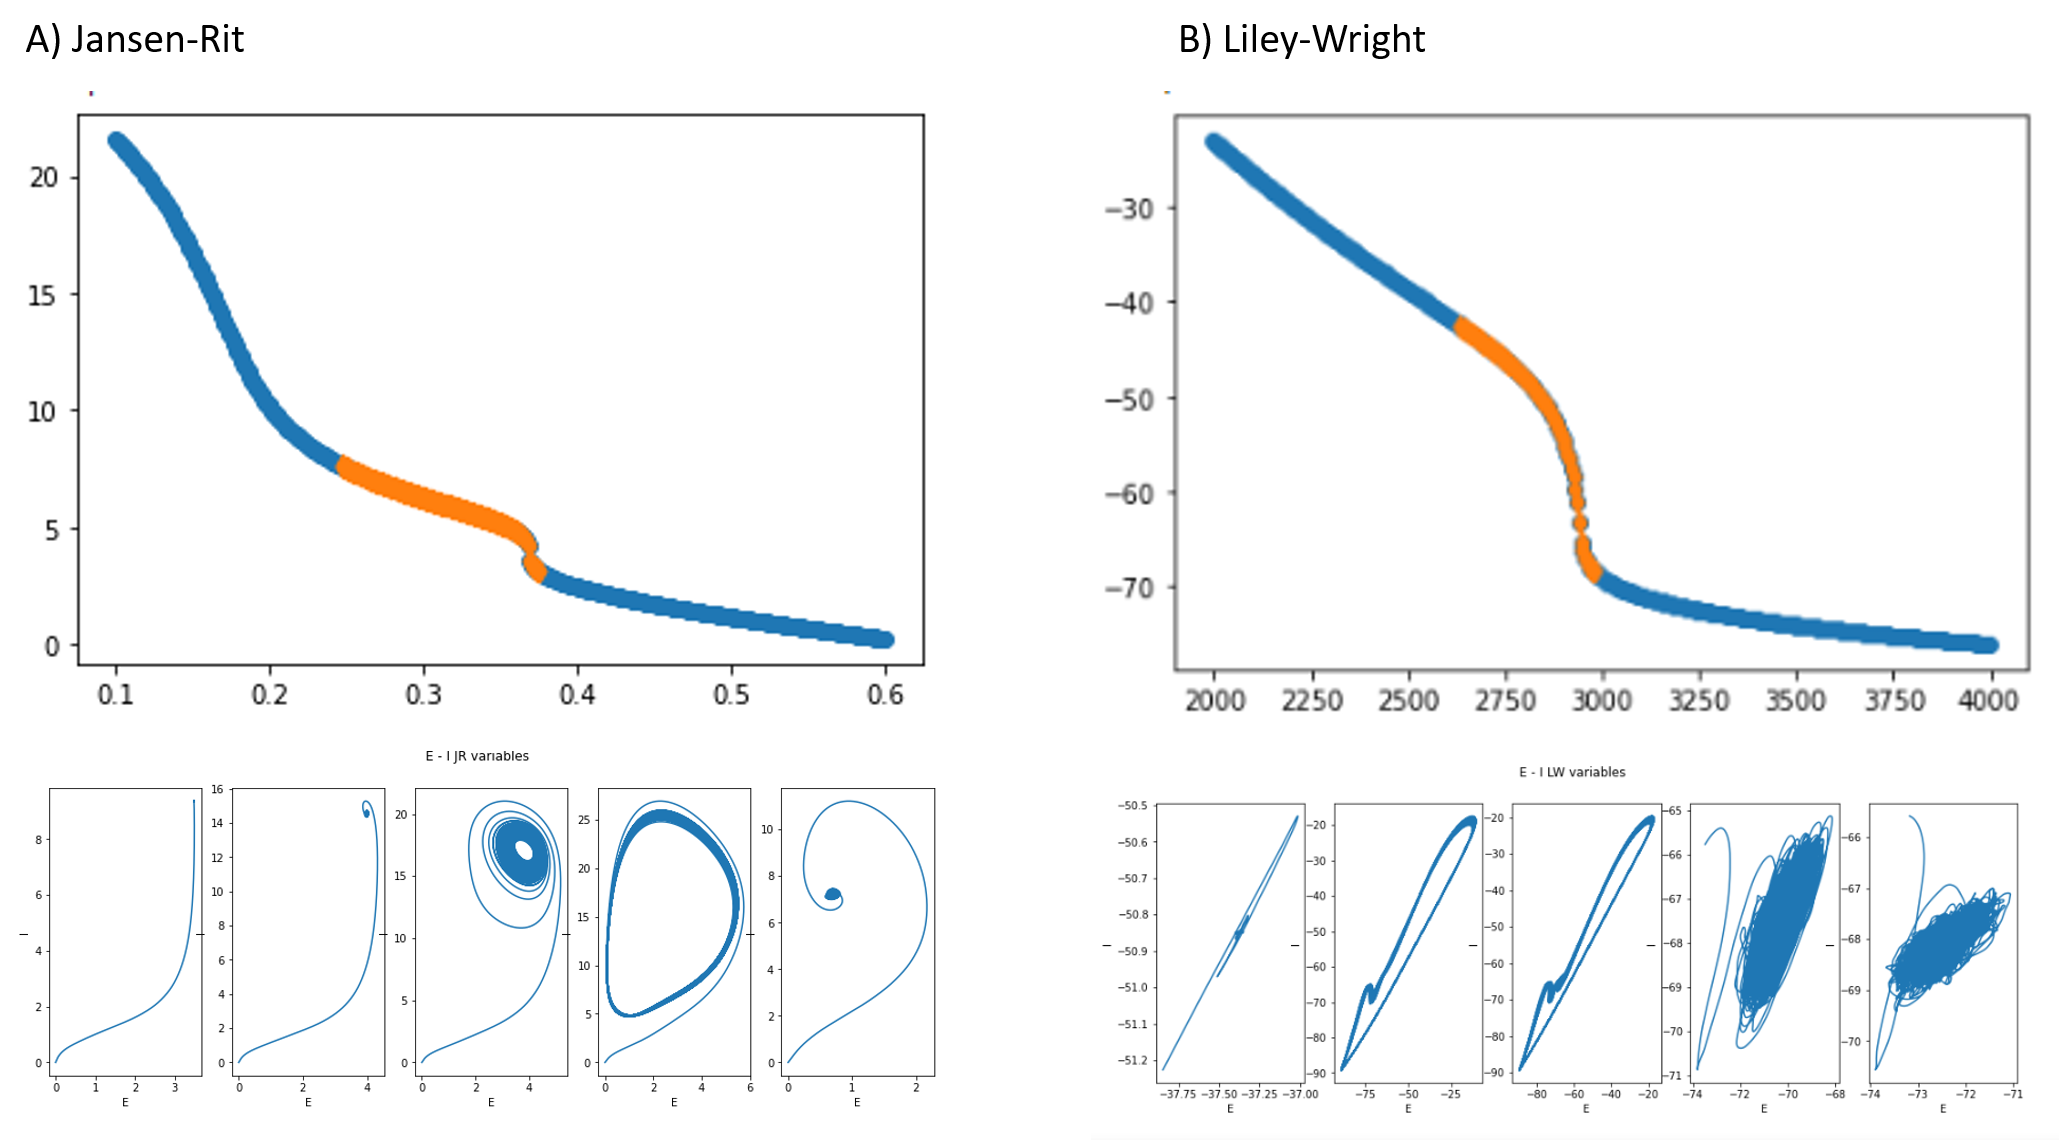
\includegraphics[scale=0.49]{Images/bifurcation_trest.png}
   % \caption*{\textbf{Figure [insert].  \textit{Fixed points and phase planes of JR and LW}} more detailed explanation} \label{fig:Fixed_points}
%\end{figure}
%TC:ignore
\begin{figure}[H]
    \hspace*{-2cm}
    %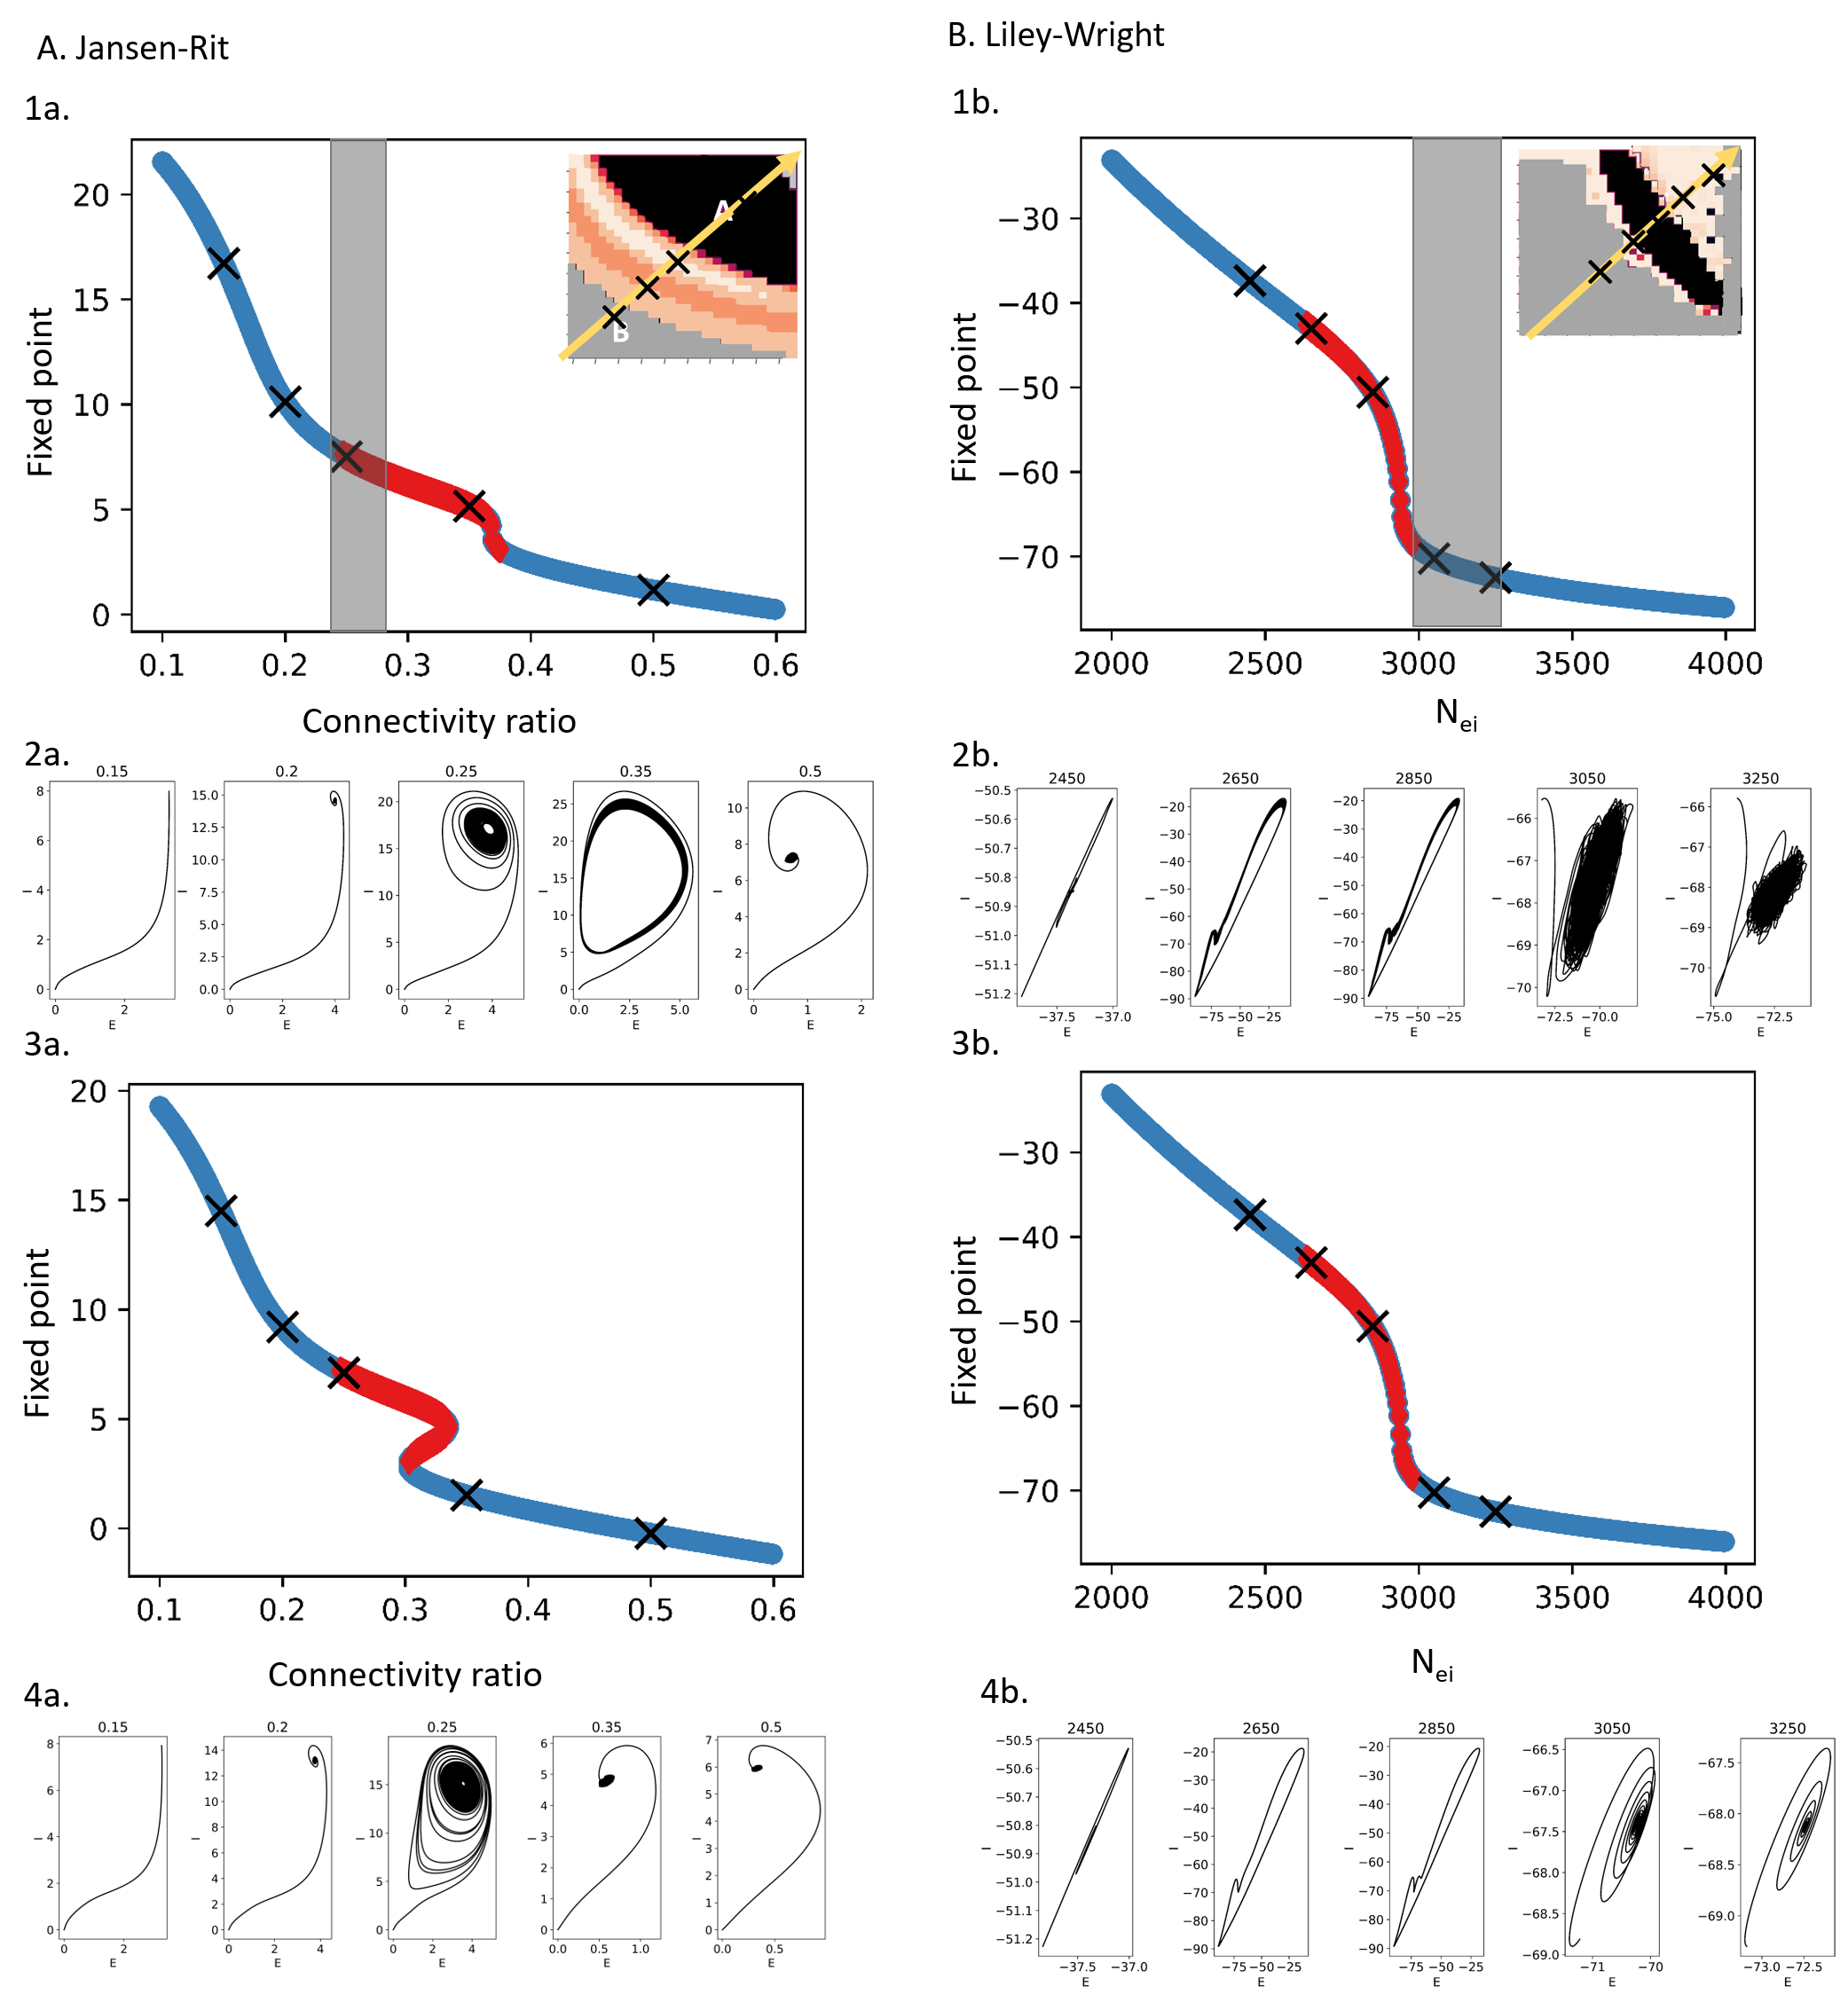
\includegraphics[scale=0.49]{Images/Stability_3.png}
    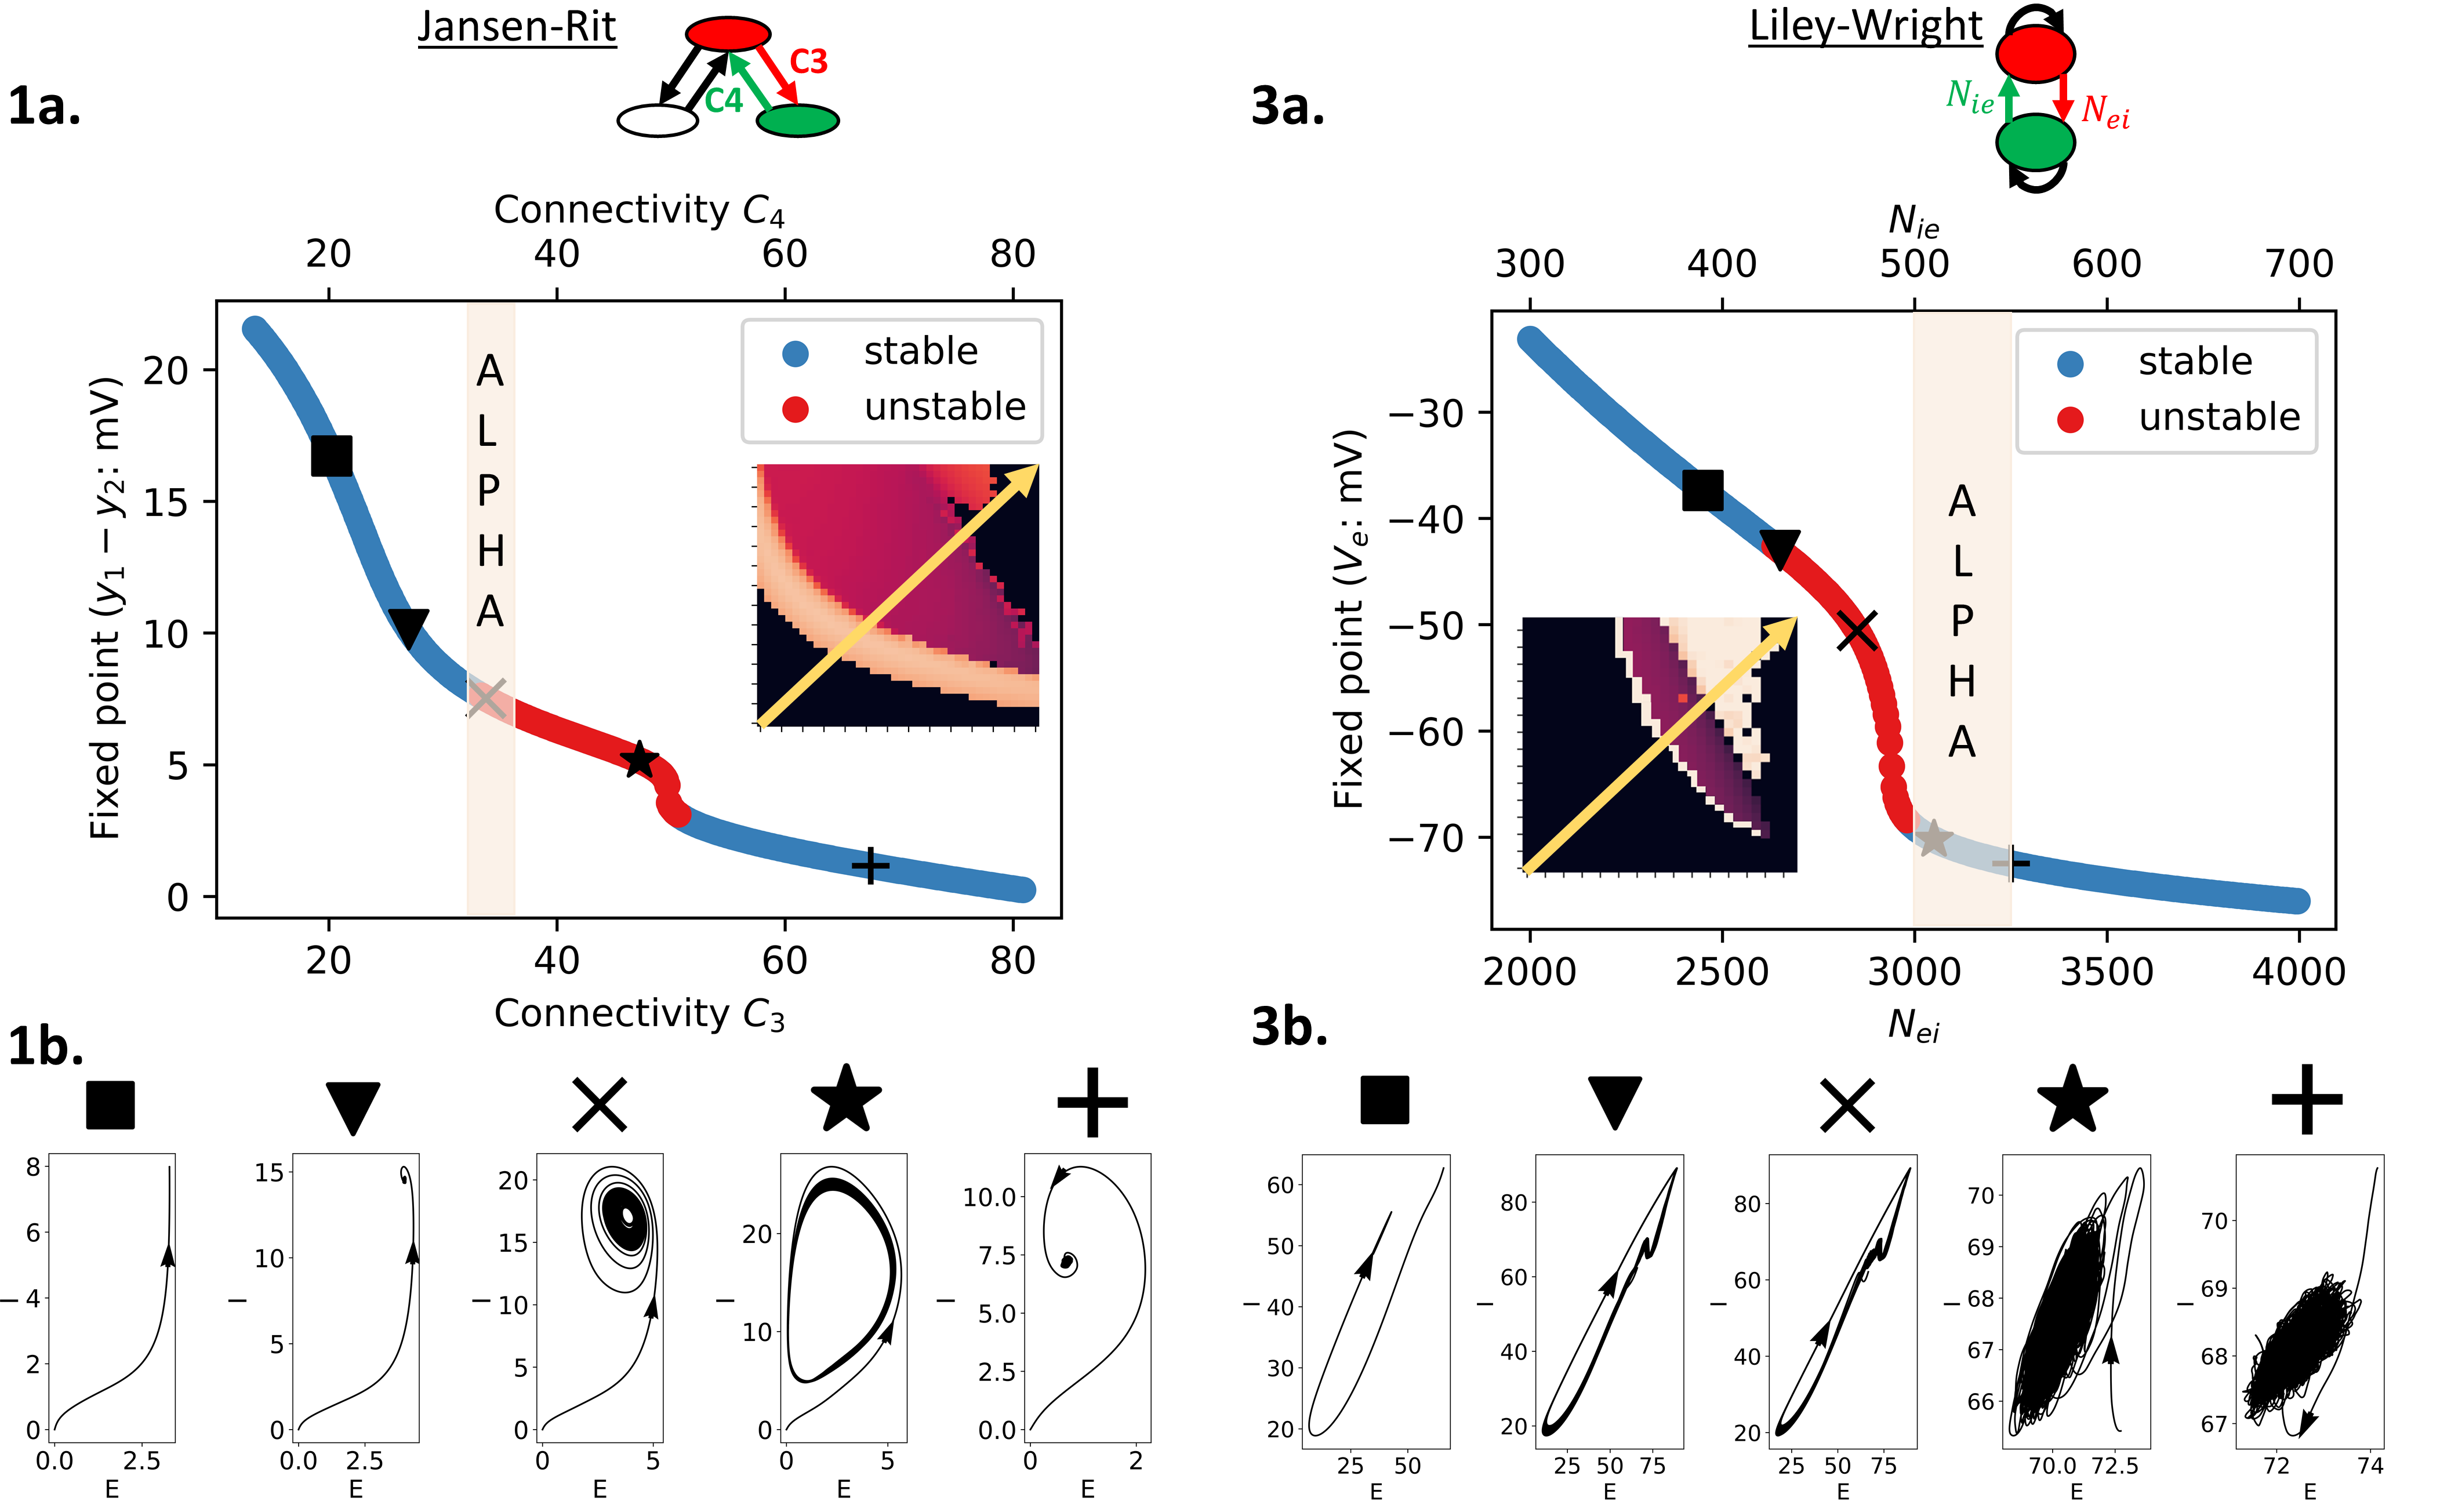
\includegraphics[scale=0.49]{Images/Stability_noise_2.png}
    \hspace*{-0.3cm}
    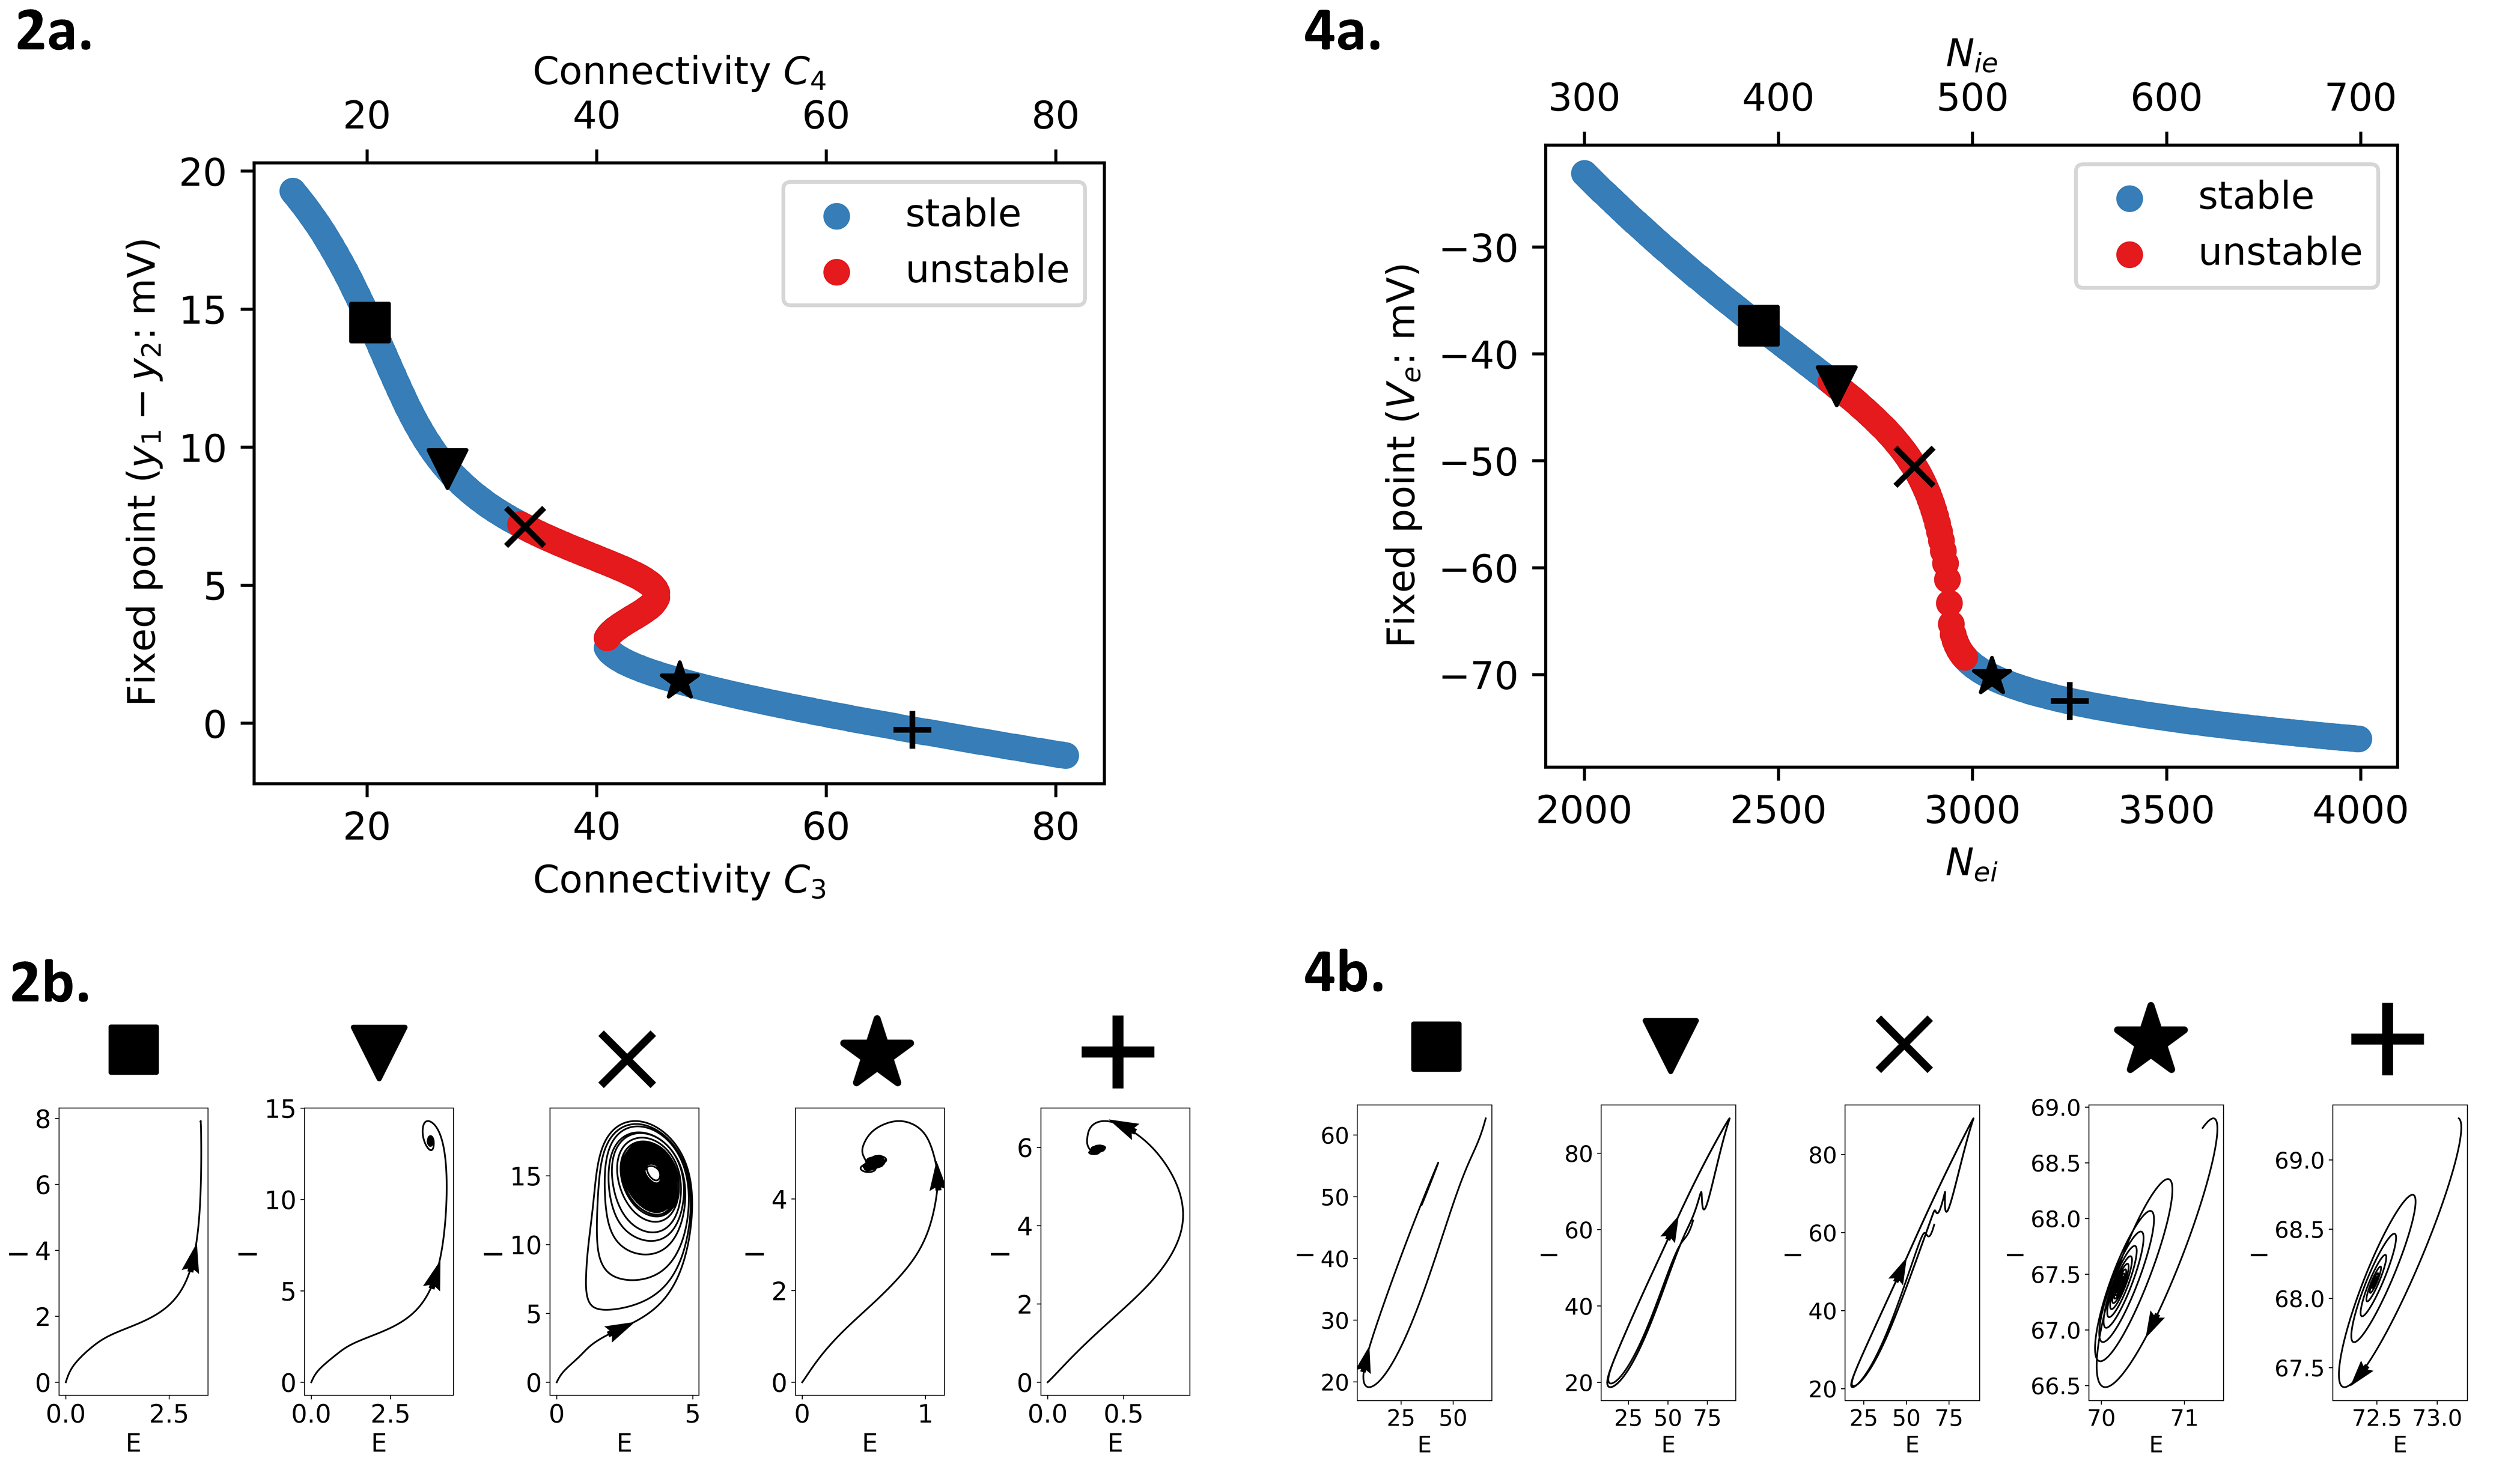
\includegraphics[scale=0.49]{Images/Stability_low_noise_2.png}
    \caption*{\textbf{Figure 12.  \textit{Fixed points and corresponding phase planes of JR and LW at specific connectivity values with high and low noise}} By performing stability analysis, the stability of the fixed points of JR and LW is determined for connectivity values intersecting across the parameter space (yellow arrow). For the JR model, \textbf{1a} and \textbf{2a} correspond to the fixed points of JR with noise and low noise, respectively, as well as their phase planes for specific values of connectivity in \textbf{1b} and \textbf{2b}. Similarly to JR, in \textbf{3a} and \textbf{4a} the fixed points of LW with noise and no noise are presented with the corresponding phase planes in \textbf{3b} and \textbf{4b}. Unstable fixed points are red, whereas stable fixed points are blue. The light orange area corresponds to the optimal connectivity parameter setting to generate alpha oscillations in each model.} \label{fig:Fixed_points}
\end{figure}
%TC:endignore
These findings enhance our understanding of the relationship between E-I connectivity, alpha oscillations, and the specific mechanisms at play in the LW and JR models. They emphasize the importance of striking a balance in synaptic connectivity and shed light on the key role of cortico-thalamic interactions in generating and modulating alpha rhythms.
%TC:ignore
\subsection{Comparative evaluation of models}
%TC:endignore

Initially, our investigation involved comparing the models within the alpha regime and conducting parameter space searches to explore the different dynamical regimes. However, we have not yet explicitly compared the various components that constitute the models, including their topology, equation formulation, and parameter values. The subsequent section of our study aims to address these aspects and critically evaluate the validity of the choices made by each model. A detailed analysis of these factors is also of central importance in understanding and assessing the suitability of the respective models as theories of alpha rhythm generation.
% Our first results consisted of comparing the models in the alpha regime and explore the dynamical regimes through parameter space searches of parameters with equivalent significance. However, the various components making the models have not be explicitly compared yet, more specifically topology, equation formulation and parameter values. The next section delves into these aspects and discusses the validity of the choices made by each model.

%TC:ignore
\subsubsection{Topology}
%TC:endignore
Patches of neural tissue, such as the cortical columns (also known as a macrocolumns) typically of interest in NPMs, comprise large numbers of both excitatory and inhibitory neurons that give rise to EPSPs and IPSPs, respectively. Therefore, NPMs commonly have at least a two population structure. Across the models surveyed in the present work, the most minimal topologically speaking is the LW model, which includes a single excitatory and a single inhibitory population only. Despite this simplicity, the LW is able to capture the balance between excitatory and inhibitory activity, while also including finer biological details such as synaptic reversal potentials and transmitter kinetics (e.g., `fast' AMPA and `fast' GABA). The LW model consists of four connections overall, including a self-connection for each population.%Therefore, the simplest possible topology of a NPM consists of two populations.\\

While the LW model, characterized by a simple structure with only a single excitatory and inhibitory population, effectively captures the balance between excitatory and inhibitory activity, there is also an interest in incorporating more neural populations to account for specific dynamics, such as adding an excitatory population. The majority of the electrical activity recorded with EEG is generated by groups of pyramidal cells \citep{louis2016appendix}, as they are the primary excitatory neuron in the brain, making up approximately 70 to 90\% of all neurons in the cortex \citep{elston2007specialization}. They are predominantly found in layers three and five of the cerebral cortex \citep{louis2016appendix}. In the JR model, pyramidal cells are separately represented from other excitatory interneurons (commonly referred to as spiny stellate cells, mostly found in layer 4; \citealp{david2006mechanisms}), yielding a model composed of three neural populations - one greater than the LW model. This additional excitatory population, and thus excitatory feedback loop stems from Katznelson's approach to explore the importance of (long-range) excitatory connections \citep{jansen1993neurophysiologically,katznelson1981normal}. Pyramidal cells interact with both excitatory and inhibitory interneurons, resulting in a total of four connections in the model. Thus, despite the difference in the number of neural populations between JR (three) and LW (two), they do have the same number of connections. This is due to the absence of self-connections in JR. In contrast, the MDF model, which shares a similar topology to JR, introduces a self connection to its inhibitory population. This extension is motivated by experimental and theoretical evidence suggesting the necessity of such connections for high-frequency oscillations in the gamma band \citep{moran2007neural}. The corticothalamic RRW model is composed of four neural populations: excitatory and inhibitory neurons in the cortex, and the (excitatory) relay and (inhibitory) reticular nuclei of the thalamus. Regarding cortical connectivities, is is assumed that the number of projections from each source neuron to each target population is proportional to the size of the target population. This leads to $\nu_{ee} = \nu_{ie}$, $\nu_{ei} = \nu_{ii}$, and $\nu_{es} = \nu_{is}$ implying that $V_{i} = V_{e}$ and the inhibitory quantities are re-expressed in terms of excitatory quantities \citep{zhao2015generalized}. Consequently, the intracortical connections correspond to $\nu_{ee}$ and $\nu_{ei}$, representing the self-connection and the inhibitory input to the excitatory population respectively. The RRW model circuit has seven connections in total, with a single cortical output that extends to the thalamus. The reticular nucleus receives these inputs from the cortex, as well as a reciprocal connection from the thalamic relay nuclei. The four-node RRW topology can thus be summarized in terms of three primary loops: 1) an intrathalamic loop connecting the reticular nucleus and relay nuclei, 2) a direct corticothalamic loop linking the cortex and relay nuclei, and 3) an indirect corticothalamic loop involving the cortex, reticular nucleus, relay nuclei, and completing the circuit back to the cortex.
%TC:ignore
\subsubsection{Equations}
%TC:endignore
As noted previously, all of the models studied here characterize neural subpopulation activity within their respective circuits using at least one second-order (equivalently, two first-order) differential equation(s), combined with a nonlinear operator that describes the synapses and postsynaptic dendritic processes \citep{ABURN}.

Three sets of two first-order differential equations are defined to describe each neural population in JR. The model assumes that excitatory and inhibitory interneurons have identical states up to a scaling constant \citep{ABURN}, and pyramidal neurons synapse equally onto the excitatory and inhibitory populations \citep{cook2021neural}. Mathematically, this implies that the contributions from EPSPs and IPSPs are not separately simulated for the pyramidal population, unlike the MDF model. In the MDF model, the contributions from excitatory and inhibitory populations are separately calculated to give rise to EPSPs and IPSPs. The difference between the two results in a mixture of potentials induced by excitatory and inhibitory currents, which  equates to the measured local field potential \citep{moran2007neural}. Additionally, the MDF model incorporates recurrent connections in the inhibitory population. This means that, compared to the JR model, the MDF model includes two additional differential equations, and the measured response corresponds to the difference between EPSPs and IPSPs. \\
Furthermore, MDF is distinguished from the other models by its richer and more flexible sigmoid function definition, in terms of two parameters ($\rho_{1}$ and $\rho_{2}$) that determine its shape (voltage sensitivity) and position respectively. The MDF model also has the possibility to include adaptation currents, through a parameter $a$ which is set to 0 in our analyses.

Mathematically, the LW model is slightly more complex than the other three models studied here, mainly due to its inclusion of an additional block for each subpopulation that converts post-synaptic potentials into the soma membrane potential, allowing for the inclusion of synaptic reversal potential terms in the equations. The model consists of three distinct blocks that perform specific transformations. The first block transforms the soma membrane potential into firing rate with a nonlinear operator in the form of a sigmoid, as described in the methods section. In the second block, the firing rate is converted into postsynaptic potential on the target population (i.e. on $I$ for the $E \rightarrow I$ and  $I \rightarrow I$ connections, and on $E$ for the $I \rightarrow E$ and $E \rightarrow E$ connections), representing the integrated effect of synaptic inputs. Finally, the postsynaptic potential is further translated into the soma membrane potential, modelled in this case according to conductance-based rules \citep{song2019novel}. Unlike the other models, LW thus has two state variables for each population: the postsynaptic potential and the soma membrane potential. LW also includes fast excitatory and inhibitory neurotransmitter kinetics not found in JR, MDF, or RRW. 

In the RRW model, activity dynamics are nominally specified in four neural populations: cortical excitatory, cortical inhibitory, thalamic reticular, and thalamic relay neurons \citep{robinson2002dynamics}. However, as noted above, with the assumptions made in this case, the two cortical populations are not clearly separated into specific subgroups within the equations. As a result, there are no local inhibitory connections within the cortex, and only one cortical output extends to the thalamic populations - reducing the number of equations as compared for example to LW, which is a fully connected graph. The equations that govern the RRW model first describe the firing behavior of individual cells within each population. These firing cells serve as sources of pulse fields, which are treated as average spike rates in their respective populations. The propagation expressed as a damped wave equation in the RRW model, which is only taken into consideration for the cortical excitatory population since it is the only one with a finite $\gamma_e$, is what differentiates it from the other models. Therefore, mathematically, we observe that there is an additional $\phi_e$ term corresponding to the average pulse density, nonexistent in the other neural populations or models. 

%The inputs from these spike rate fields are then filtered by the dendrites of postsynaptic neurons before reaching the cell body, where the membrane potential is determined. Subsequently, the membrane potential of each population's neurons determines the firing rate of that population. The firing rate, in turn, propagates to other populations within the model. To summarize, the average cell body voltage in each population serves as a trigger for the firing rate, which generates outgoing activity that propagates to other populations. As the activity propagates, it is filtered by the dendritic structures, ultimately producing a cell-body voltage for each population in the model \citep{robinson2002dynamics}.
%TC:ignore
\subsubsection{Unified parameter table}
%TC:endignore
One of the aims when developing and studying mathematical models, such as the four considered in the present work, is to relate various model parameters to specific biological features or processes of the brain, and in so doing to more fully understand the mechanisms underlying neural activity, as well as how changes in these factors may impact brain function and behavior. This can include features such as the properties of individual neurons or synapses, the architecture of neural circuits, or the dynamics of different neural populations. Unfortunately however, this task can sometimes be a challenging one for NPMs, since many of the models in common use today (including all four reviewed in this paper) were formulated phenomenologically - i.e. via a top-down strategy focused on replicating activity dynamics in neural recordings, rather than the fine-grained details of neuronal circuit microstructure. 

It is therefore, necessary to understand the role of the different elements and the rationale behind the choice in their values, to make them as biophysically meaningful and interpretable as possible. To aid with this, Supplementary S.6 includes a set of tables with a brief description of each model's parameters and their biological meaning. Although the models do often have slightly different values for corresponding parameters, they do nevertheless often share similar functional roles. To facilitate further comparison, an additional table is given below that aims to relate variables of equivalent biological meaning (Table 2).

Among the JR, RRW, and LW models, which use very similar expressions for their sigmoidal transfer functions, there are three key common parameters that emerge: i) mean firing threshold, ii) firing threshold variability, and iii) maximum attainable firing rate. JR, MDF, and LW, which include both a separate excitatory and inhibitory impulse response function, have the following shared components: maximum amplitude of EPSPs, and of IPSPs, and an excitatory and inhibitory rate constants. Finally, every model has features representing the connections between neural populations. The MDF model introduces additional parameters to define the shape of the sigmoid function used in its formulation, providing easier modulation of the shape of the sigmoid compared to the other models. In RRW, the impulse response differs, which includes a decay and rise time of the impulse response, affecting the dynamics of the model's dendritic filtering process. Furthermore, factors associated with corticothalamic interactions are introduced in the RRW model to account for long-range interactions between cortical and thalamic regions. The LW model distinguishes itself by incorporating attributes related to synaptic reversal potentials, such as the resting membrane potential and passive membrane decay time constant. These parameters are essential for transforming the postsynaptic potential into the soma membrane potential and incorporating synaptic reversal potentials into the model's dynamics. 

%\begin{figure}[H]
%\centering
   % 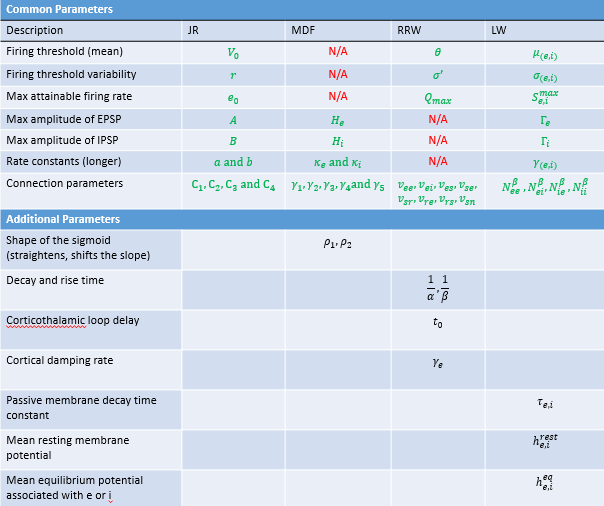
\includegraphics[width=0.95\linewidth]{Images/Unified_Param_Table.png}
   % \caption*{\textbf{Figure 25.  \textit{Table unifying parameters across models based on their biological interpretation.}} Common parameters are highlighted in green. JR,  }     
   % \label{fig:Param_Table}
%\end{figure}

%\rowcolors{2}{gray!20}{gray!70}
\begin{table}[thb]
    \centering
    \begin{tabular}{ccccc}
        \rowcolor{black} 
        \multicolumn{5}{|c|}{\textcolor{white}{Common Parameters}} \\
        \hline
        \rowcolor{gray!70}
        Model & JR & MDF & LW & RRW \\
        \rowcolor{gray!20}
        Firing threshold (mean) & $V_{0}$ & -- & $\mu_{e,i}$ & $\Theta$   \\
        \rowcolor{gray!70}
        Firing threshold variability & $1/r$ & -- &  $\sigma_{e,i}$ & $\sigma'$\\
        \rowcolor{gray!20}
        Maximum firing rate & $2e_{0}$ & -- & $S_{e,i}^{max}$ & $Q_{max}$ \\
        \rowcolor{gray!70}
        Maximum EPSP amplitude & $A$ & $H_{e}$ & $\Gamma_{e}$ & -- \\
        \rowcolor{gray!20}
        Maximum IPSP amplitude & $B$ & $H_{i}$ &  $\Gamma_{i}$ & -- \\
        \rowcolor{gray!70}
        Rate constants & $a$ and $b$ & $\kappa_{e}$ and $\kappa_{i}$ &$\gamma_{e,i}$ & --  \\
        \rowcolor{gray!20}
         &  &  &  & $\nu_{ee}, \nu_{ei}, \nu_{es}, \nu_{se}$\\
        \rowcolor{gray!20}
        \multirow{-2}{*}{Connectivity} & \multirow{-2}{*}{$C_{1}, C_{2}, C_{3}, C_{4}$} & \multirow{-2}{*}{$\gamma_{1}, \gamma_{2}, \gamma_{3}, \gamma_{4}$} & \multirow{-2}{*}{$N_{ee}^{\beta}, N_{ei}^{\beta}, N_{ie}^{\beta}, N_{ii}^{\beta}$} & $\nu_{sr}, \nu_{rs}, \nu_{re}, \nu_{sn}$ \\ 
        \rowcolor{black} 
        \multicolumn{5}{|c|}{\textcolor{white}{Additional Parameters}} \\
        \rowcolor{gray!70}
        Sigmoid shape & & $\rho_{1}, \rho_{2}$ &  &  \\
        \rowcolor{gray!20}
        Decay and rise time & & & & $\frac{1}{\alpha},\frac{1}{\beta}$ \\
        \rowcolor{gray!70}
        Corticothalamic loop delay & & & & $t_{0}$ \\
        \rowcolor{gray!20}
        Cortical damping rate & & & & $\gamma_{e}$ \\
        \rowcolor{gray!70}
        Passive membrane decay & & & & \\
        \rowcolor{gray!70}
        time constant & & &\multirow{-2}{*}{$\gamma_{e,i}$} &\\
        \rowcolor{gray!20}
        Mean resting  & & & & \\
        \rowcolor{gray!20}
        membrane potential & & & \multirow{-2}{*}{$h_{e,i}^{rest}$}& \\
        \rowcolor{gray!70}
        Mean equilibrium potential & & & $h_{e,i}^{eq}$& \\
    \end{tabular}
        \caption*{\textbf{Table 2.  \textit{Common parameters across models based on their biological interpretation.}} Certain parameters have a similar role and a biological interpretation associated with it that is comparable between the models. The additional parameters reflect the novelty and differences proposed by each models.}  
    \label{tab:global_eval}
\end{table}


%TC:ignore
\subsubsection{Deciphering the biological basis and rationale of parameter values}
%TC:endignore
The systems under consideration have parameters with corresponding biological interpretations; however, the nominal values assigned to these parameters vary considerably across the models. The variation in parameter values across the models can be attributed to several factors, including differences in the experimental data used to inform the models, distinct mathematical formulations, and specific assumptions. Each model is designed to capture different aspects of neural activity and may prioritize certain features or phenomena over others. In the following section, we first examine the rationale behind the expression and parameters of the firing rate function, then the impulse response, and finally the connectivity values. 

%Even though MDF is an extension of JR, in \citet{moran2007neural}, the authors deliberately selected `standard' parameters that prioritize an engaged synchronized EEG with significant power in the higher beta frequency range, aiming to showcase the impact of nonlinearities in their computational framework. The standard MDF parameters are thus adjusted here to place the central frequency in the alpha band by using comparable values \citet{david2003neural}. %or is it David and Friston 2005 
%herefore, parameter values of JR and MDF impulse response and firing rate function are of the same order, and can be traced back to three key authors: \citet{freeman1974model, freeman1975mass, freeman1987simulation, freeman1979nonlinear}, \citet{lopes1974model, da1976models}, and \citet{van1982model}.
%As mentioned in section 2.2.1, Freeman's work is a source for numerous parameter values in NPMs, which were empirically assessed based on detailed physiological studies of the olfactory bulb. 

\paragraph{Firing rate} ~\\
Fig. 13 shows the firing rate curves of the four models. It can be seen here that there is some variability in maximum neural firing rate parameters used, as well as the point of inflection of the curves. As mentioned in the previous section, MDF implements a different expression of the sigmoid that does not include parameters equivalent to a maximum firing rate, mean firing threshold, or standard deviation of the threshold distribution in the neural population, but instead has two parameters defining shape and position. The maximum amplitude with the current setting reaches 0.9, but can be tuned by modifying the parameters $\rho_2$. Even though the other three models have parameters with a similar biological interpretation, the values are considerably different. First, the maximal firing rate is equal to $500s^{-1}$, $340s^{-1}$ and $5s^{-1}$ for LW, RRW and JR respectively. The difference in the order of magnitude between JR and the other two models (LW and RRW) can in part be explained by the fact that the value chosen by Jansen and Rit in their original paper is taken from \citet{freeman1987simulation}, and is actually a dimensionless normalized parameter. This quantity is expressed without units (for details on the calculation of the maximal wave amplitude $Q_{m}$ see \citealp{freeman1979nonlinear}), whereas both RRW and LW rely on experimentally derived average values. However, in the case of RRW, the assumed $Q_{max}$ value was made without a clear citation mentioning it is an assumption and within units of the measured maximum value possible \citep{robinson1997propagation, rennie1999effects}. The standard values from Freeman for converting membrane potential to firing rates are applied in the JR firing rate function, but the expression itself stems from \citet{da1976models}, and the current JR model uses a simplified version of that function. In the case of RRW, the firing rate function initially corresponded to the error function introduced by \citet{wright1995simulation}. Since 1999, the nonlinear function in the RRW model has been a modified version of that initial error function and closely approximates it \citep{rennie1999effects}. The differing source of the firing rate conversion equation between the two models explains the slight differences observed in their mathematical expressions. 

%Whereas, RRW and LW values are averages found experimentally. Although, for RRW, it is mentioned that the value of $Q_{max}$ is an assumption that was made (source) and no source seems to be cited.
The spiking threshold parameter (voltage at point of inflection in the sigmoid curve) in LW has a negative potential, due to the fact that the model includes synaptic reversal potentials. JR and RRW, in contrast, have a positive point of inflection for this parameter ($6mV$ and $12.92mV$ respectively). The values for the standard deviation of the threshold distribution in the neural population, which affects the steepness of the firing ate slope, are $(1/0.56)mV$ ($\approx 1.79mV$), $5.5mV$, and $5.9mV$ for JR, LW, and RRW respectively.  
%didnt talk about the variability
%TC:ignore
\begin{figure}[H]
    \hspace{-0.5cm}
    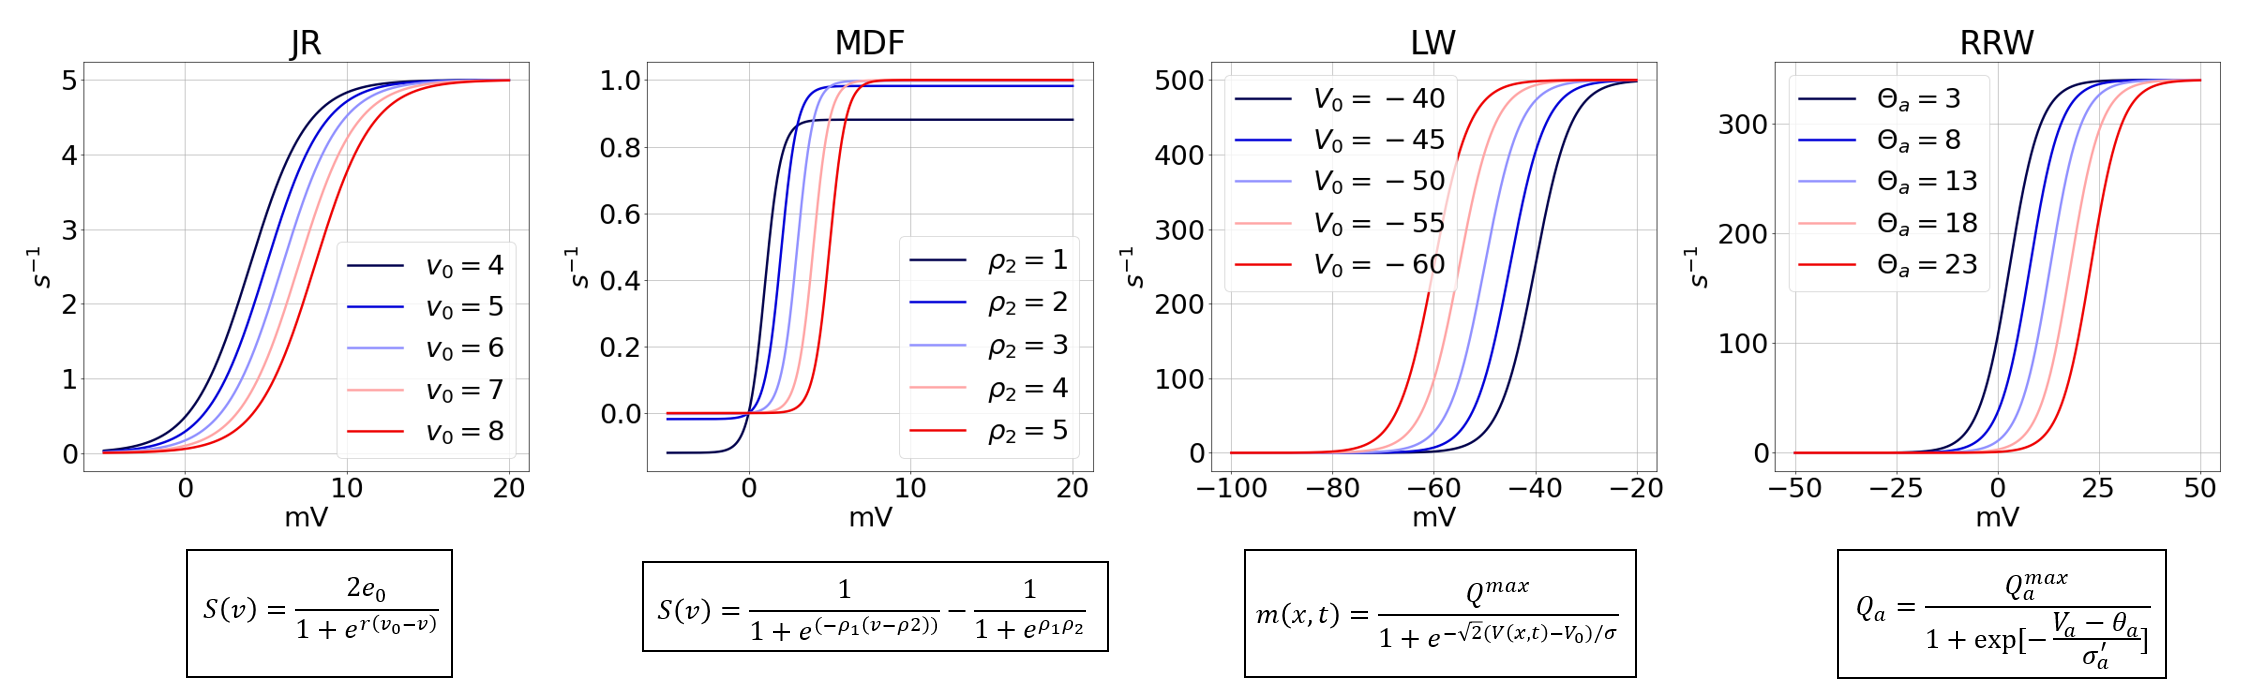
\includegraphics[scale=0.3]{Images/Sigmoid_3_1.png}
    %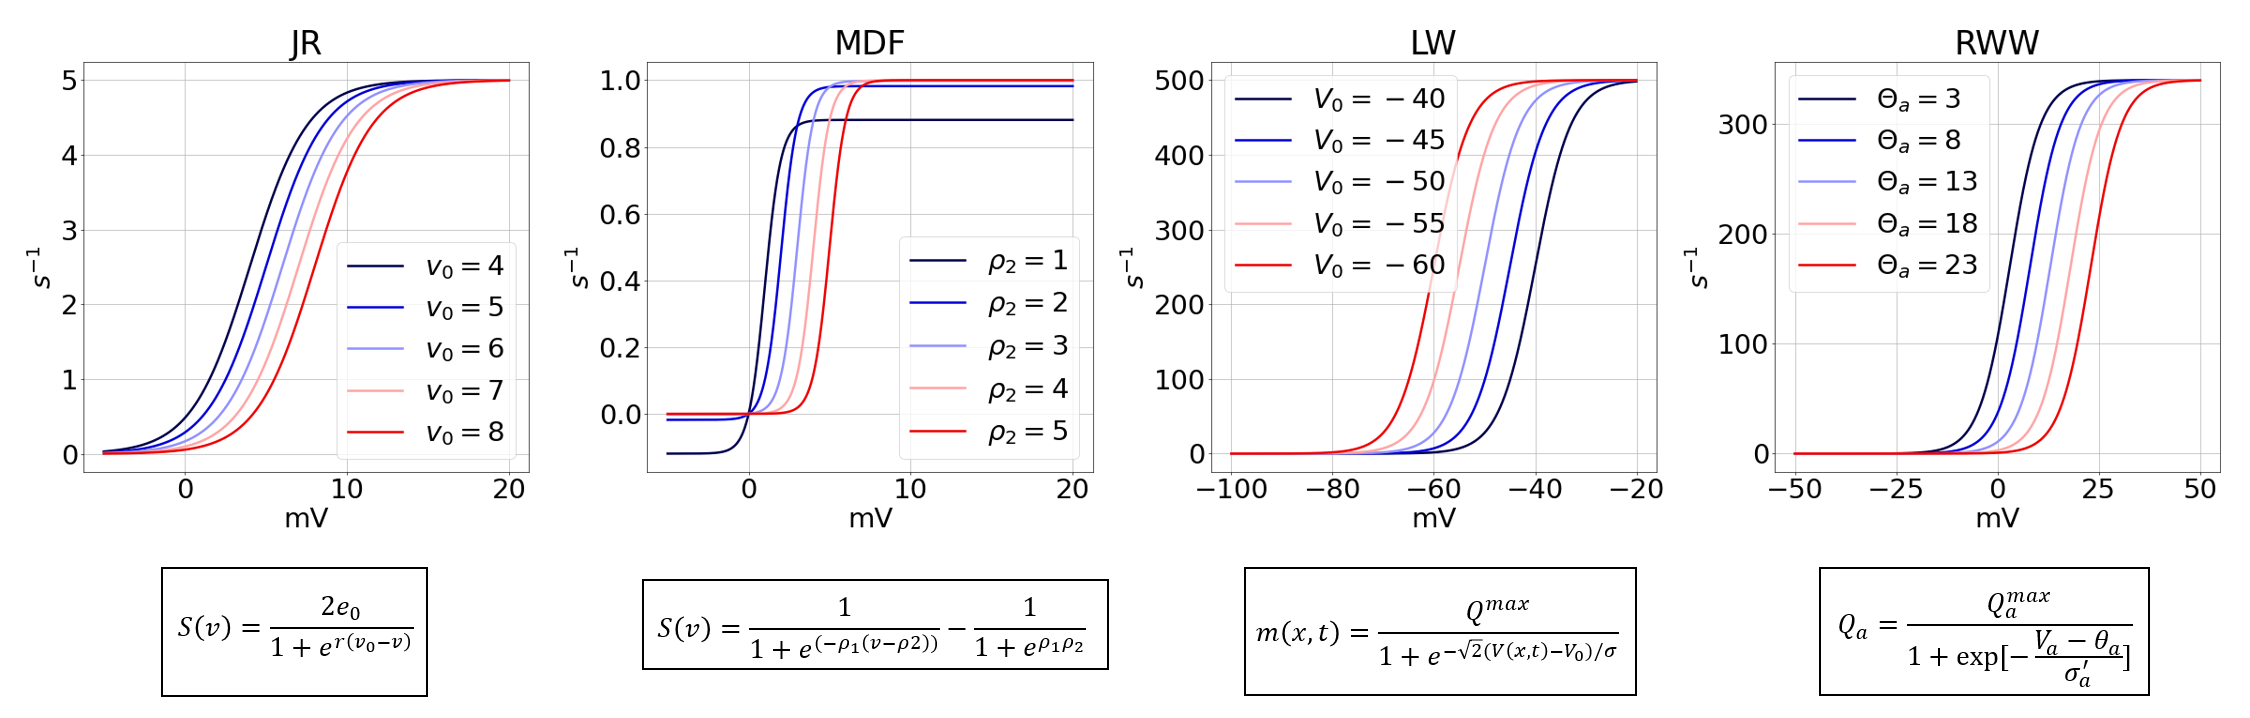
\includegraphics[scale=0.5]{Images/Sigmoid_2.png}
    \caption*{\textbf{Figure 13.  \textit{Sigmoid curve of each model with firing rate against voltage with different firing threshold.}} The sigmoids differ in terms of the maximum value and the voltage at which the inflection point occurs which is modulated by the firing threshold.}     
    \label{fig:JR_Sigmoid}
\end{figure}
%TC:endignore

\paragraph{Impulse response}~\\ 
With respect to the impulse response, the parameter values in JR can be traced back to van Rotterdam's paper in 1982 \citep{van1982model}. The impulse response used in JR corresponds to a simplified version of expression given in Lopes Da Silva \citep{lopes1974model, da1976models}. These authors determined the parameters $A$, $B$, $a$ and $b$ by respecting certain basic properties of real postsynaptic potentials, and ensuring the system produces alpha frequency oscillations \citep{grimbert2006analysis}. This choice of JR to use the alpha function (unrelated to alpha rhythms) as an impulse response was originally proposed by Rall \citep{rall1967distinguishing}. 
MDF has an identical impulse response function, but some of the standard parameter values differ because in \citet{moran2007neural}, the authors deliberately selected `standard' parameters that prioritize an EEG with significant power in the higher beta frequency range, aiming to showcase the impact of nonlinearities in their computational framework. The standard MDF parameters are thus adjusted in the present study to place the central frequency in the alpha band by using comparable values to \citet{david2003neural}. %or is it David and Friston 2005 
With our adjustments to obtain alpha oscillations, the values of the impulse response in MDF vary slightly from those in \cite{moran2007neural}, such as the rate constants ($250s^{-1}$ instead of $100s^{-1}$ for $\kappa_e$; $62.5s^{-1}$ instead of $50s^{-1}$), but are still in the same order of magnitude. These differences are explained by the fact that the additional self-inhibitory connection changes the behavior of the system for similar parameter values. Thus, to simulate an equivalent alpha these need to be modified.
%One notable difference that is in \cite{moran2007neural} is the maximum amplitude of IPSP in MDF which is equal to 22mV instead of which to the one proposed earlier by Lopes Da Silva 1974 instead of van Rotterdam (32mV instead of 22mV). --> with our modification in the end IPSP is 22 but EPSP is 10
There is some variability across the models in the values used for EPSP and IPSP amplitudes. This has been justified physiologically by the fact that certain neuropeptides can modulate the amplitude of PSPs, meaning that some degree of freedom in choice of these values is needed \citep{jansen1995electroencephalogram}.
For the dendritic response, the original RRW model paper \citep{robinson1997propagation} mentions using `physiologically reasonable parameters' for the decay and rise rate ($\alpha$ and $\beta$), and cites sources such as \citet{freeman1991induced, lopes1974model, van1982model} with no further details provided. It is surprising that the peak of the dendritic response is around 60mV, which is considerably higher than the other models. LW, on the other hand, has a lower potential peak amplitude, which can may be due the fact that other models represent the voltage at the soma, whereas LW expresses it at the site of synaptic activation \citep{liley2001spatially}. One of the status intentions of the LW model relative to its predecessors was to be more physiologically realistic, and thus allow greater biological validity and interpretability of its parameters \citep{liley2001spatially}; however it is notable that very little detail is given about the sources for chosen parameter values. %LW assumes that the parameters are time invariant. %(question is this the case for every model?). 
Overall, an anatomical assumption made is that the amplitude of the inhibitory impulse response is larger than the excitatory impulse response, due to the fact that the former have axon terminals closer to the cell body, thereby leading to larger perturbation upon synaptic transmission \citep{kandel2000principles,cook2021neural}. LW makes the (reasonable) assumption that excitatory impulses occur on a faster timescale than inhibitory impulses, which is shared with JR and MDF, but notably not with RRW. In Fig. 14, the shape of each model's excitatory and inhibitory impulse responses are shown, with their nominal varying rate constant values. As the rate constant increases, the curve widens and the decay time increases. In the case of RRW but not JR, MDF, or LW, variation of the decay time also leads to changes both slope and the magnitude of the impulse response curve.
%TC:ignore
\begin{figure}[H]
    \hspace{-0.5cm}
    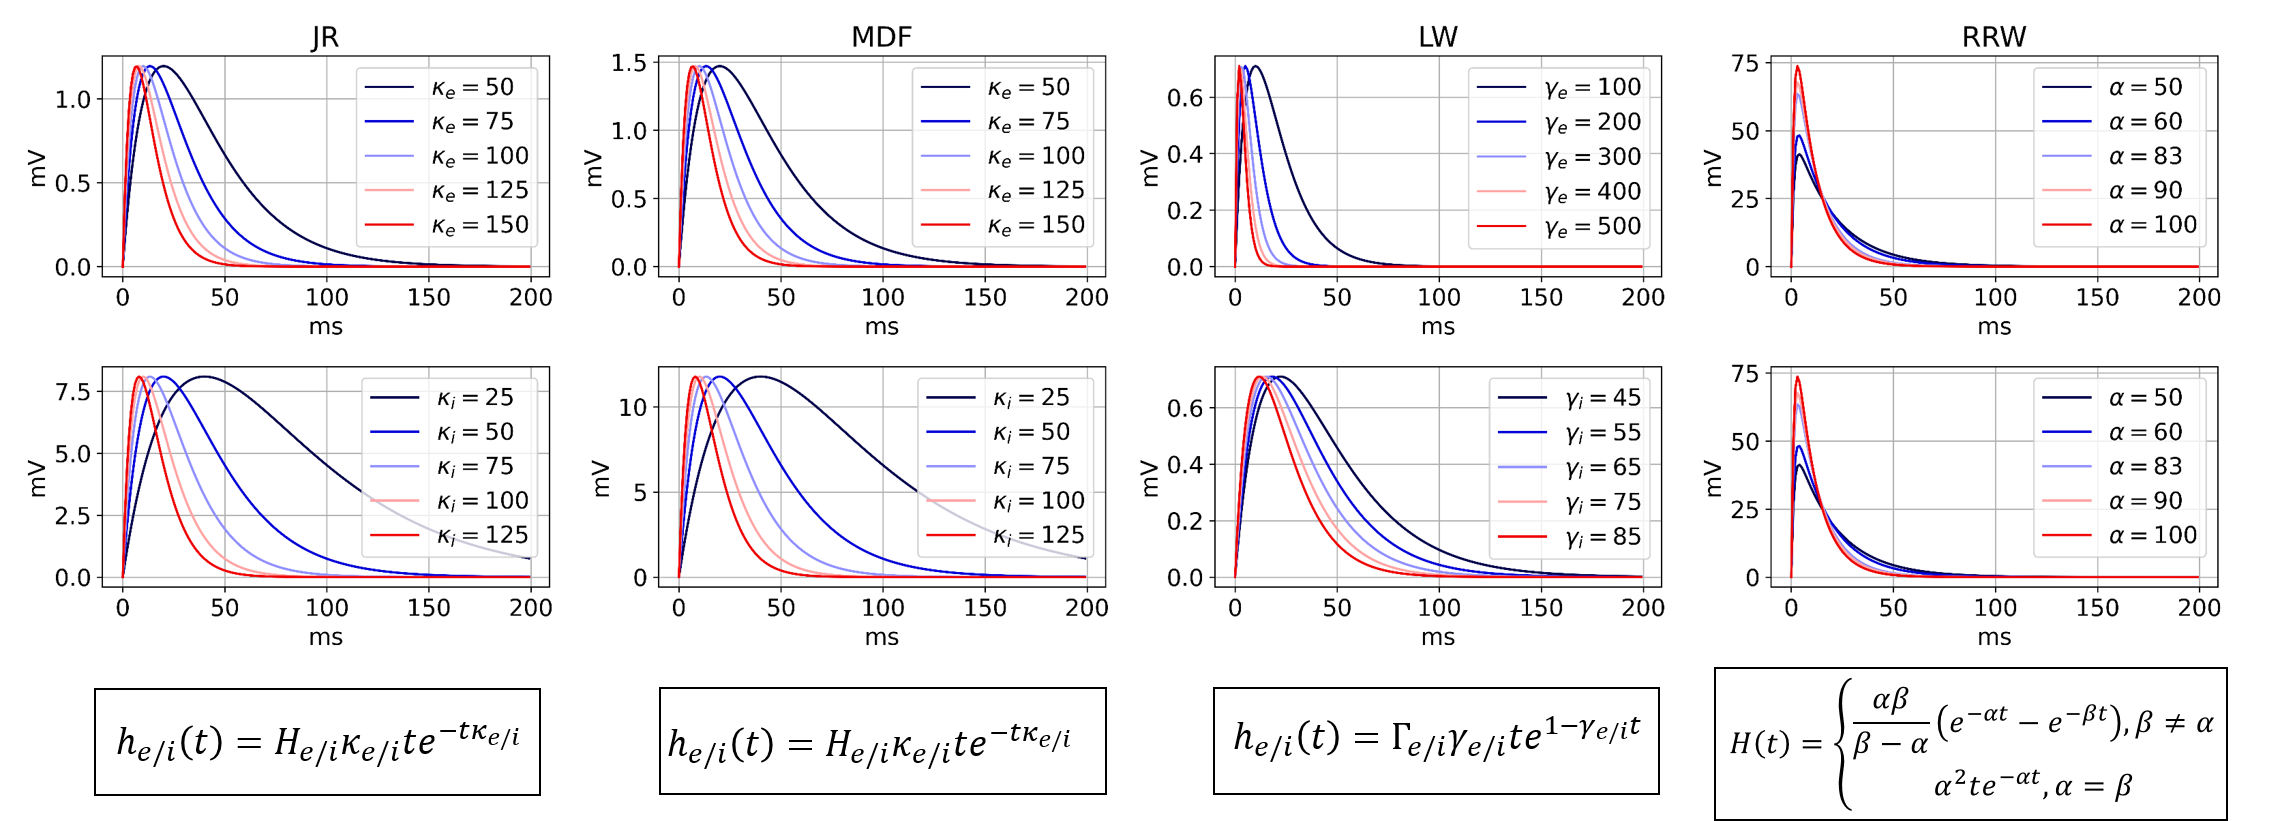
\includegraphics[scale=0.3]{Images/Impulse_response_3_1.png}
    %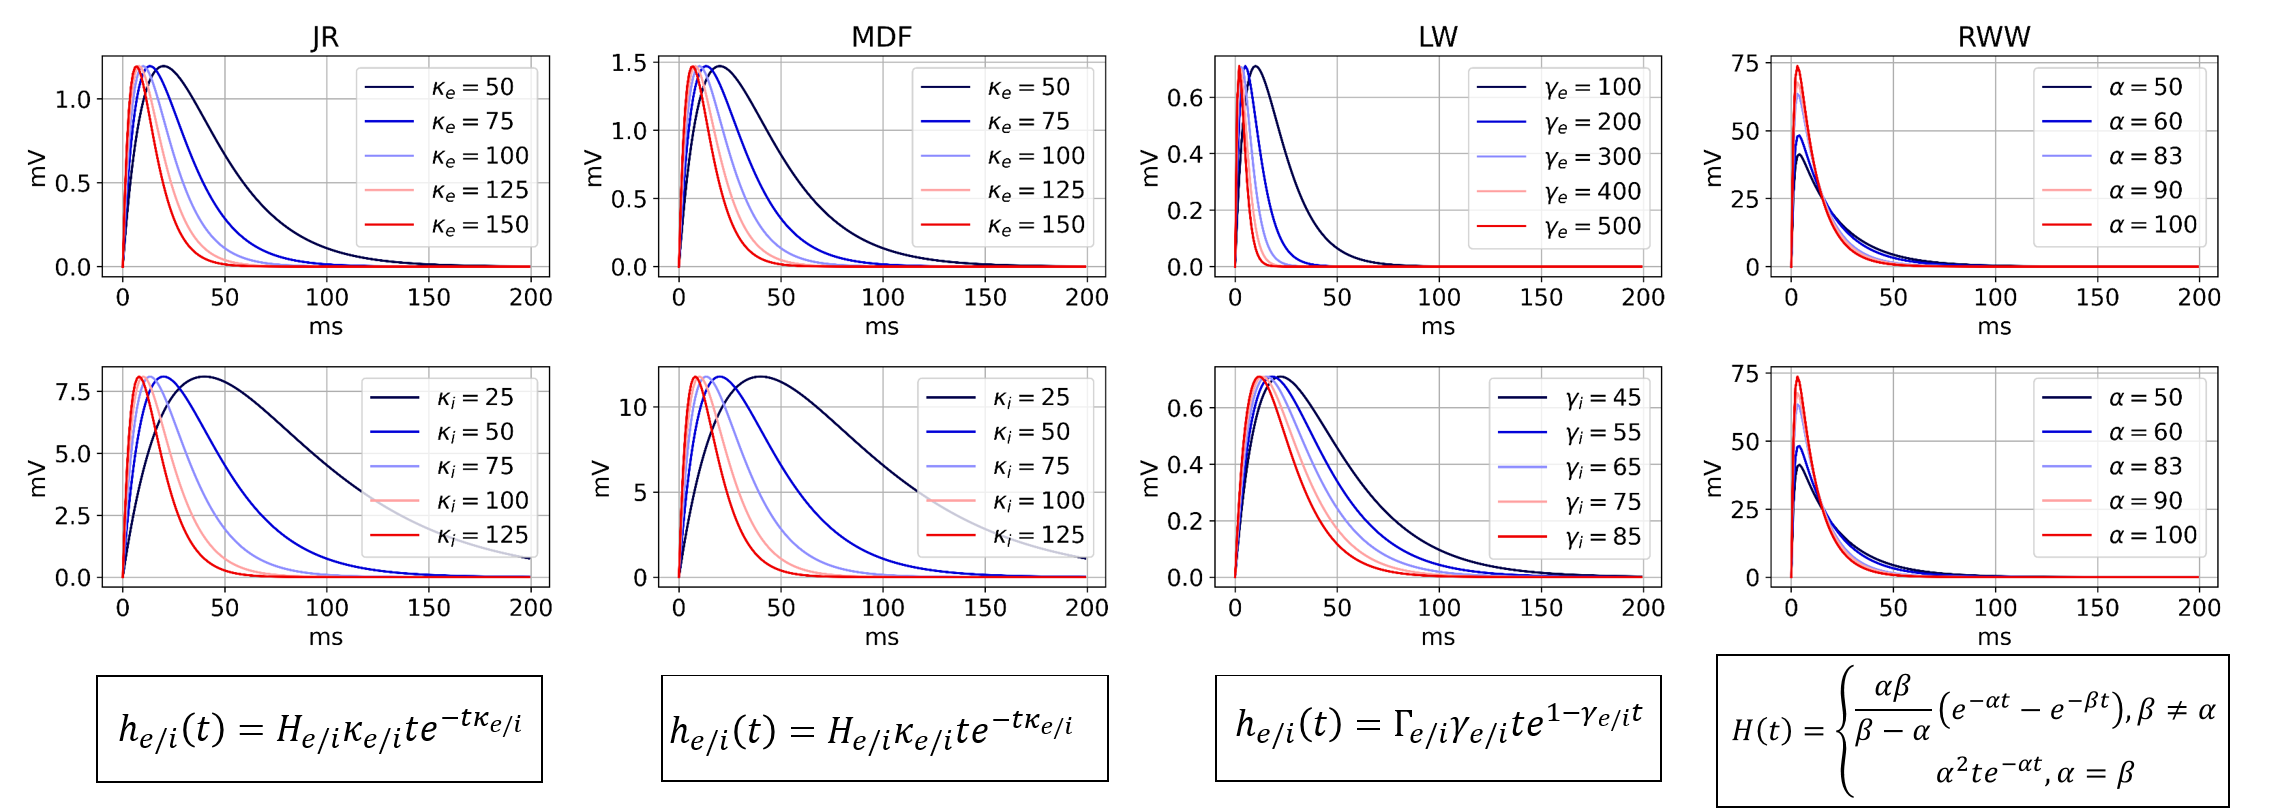
\includegraphics[scale=0.48]{Images/Impulse_response_2.png}
    \caption*{\textbf{Figure 14.  \textit{Impulse response of excitatory and inhibitory population with varying rate constant}} Top: EPSP; Bottom: IPSP; except for RRW which uses the same dendritic response curve for EPSP and IPSP. The general shape of EPSP and IPSP between the models is consistent and mainly differ in terms of amplitude. Rate constant is varied for the first three models and for RRW, the different curves correspond to varying decay times. }     
    \label{fig:JR_impulse}
\end{figure}
%TC:endignore
\paragraph{Connectivity}~\\
Connectivity parameters across the four models differ in their units and physiological interpretation, making direct comparisons of specific values challenging. In JR and MDF, the connectivity parameter values are dimensionless, and proportional to the average number of synapses between populations, thus account for the total number of synapses \citep{jansen1995electroencephalogram}. Based on several neuroanatomical studies \citep{braitenberg2013cortex, larkman1991dendritic, liu1991distribution, elhanany1990intrinsic} that estimated these quantities by counting synapses. With these studies, Jansen and Rit condensed the four connections into fractions of a single parameter C \citep{grimbert2006bifurcation}. Since Jansen and Rit estimated that the global parameter C would most likely change primarily due to its role in capturing synaptic phenomena like neurotransmitter depletion, this reduction has been useful in determining the overall effect of variations in connectivity while keeping their proportions to each other identical. LW has parameters representing the total number of connections between the two populations, which take higher values for excitatory neurons as 80\% of cortical neurons are excitatory, vs 20\% that are inhibitory neurons \citep{cook2021neural}. Furthermore, anatomical estimates for each connection were derived using an equation that considers the diameter of the mean dendrite and intracortical axon, the mean total length of all dendritic and intracortical axonal arborizations, the mean length of the pyramidal cell's basal dendritic arborizations, and the neuronal density (as described in \citealp{liley2001spatially} and outlined in \citealp{liley1994intracortical}). RRW has connectivity variables denoted as $\nu_{ab}$, which correspond to the mean number of synapses (anatomical or structural in nature) multiplied by the strength of the response to a unit signal expressed in units as $mVs$ (related to physiology or functionality) \citep{rennie1999effects, robinson1997propagation, rall1967distinguishing}. 
 
% Need transition

This section aims to compile the origin of the mathematical expressions as well as parameter values by retracing the literature, and discerning the biological associations. Our comparative evaluation has found that even though the formulation of the firing rate curves is similar between JR, LW and RRW, their mathematical origin differs, with \citet{da1976models} as a reference for JR, and the error function introduced by \citet{wright1995simulation} for LW and RRW. This explains the variations in the parameter values. Finally, our goal is to provide a comprehensive comparison across all levels for the four models. With regards to the parameters of the impulse response, some degrees of freedom are accepted, and the parameter values are mentioned to be within reasonable physiological ranges. Finally, connectivity parameters can represent a proportion of the average number of synapses (JR and MDF), a total number of synapses (LW), or synaptic strengths (RRW). Although the specific parameter values may vary for the firing rate and the impulse response, modifying them uniformly yields a consistent effect across the two curves (Figs. 13 and 14). Similarly, as shown in Fig. 11, correspondences can be made in the effects of altering connectivities.

%Additionally, the models have different regions of stability and are able to produce other types of oscillations. Defining the parameter space of those different regions for each model allows for comparison in the behavior of the system/model.
%Add effect of input and choices.


% mini summary

% - identified, described, reviewed, analyzed alternative alpha models and theories and subcomponents etc

% new things:

% - alpha blocking: robinson, used params from prev papers; liley - same; JR - new result = do what liley did
% - can we do this with analytic models in that fig also?

% - rate constants fig (jr done before but comparison w liley and moran not)
% - 

% - E vs I param space comparing over models; diagonal sweet spot; angle of diagonal = asymmetry between E and I variation; non-alpha behaviour off the diagonal (fig 11)

% fig  12 - bif analysis - all new (?)
% confirmation that alpha 'mechanism' (mathematically at least = bifurcation type) is different between JR and LW

% param comparisons (*notable points?)

% sigmoids and impulse responses - key points?

%TC:ignore
\section{Discussion}

%We compared the four prominent intracortical and corticothalamic models above to investigate the dynamics and mechanisms of alpha rhythms through local circuits. 

\subsection{Summary of main findings}
%TC:endignore
In this paper we have undertaken a systematic investigation into the major mathematically-expressed physiological theories of EEG alpha rhythmogenesis. This has centred around an in-depth comparison of four primary models (JR, MDF, LW, RRW) that predominate in the literature, which also cover the two main alpha theory types (intracortical and corticothalamic \citealp{nunez2006electric}). By clarifying at a technical and a conceptual level the relationships between the four models, our aim has been to prepare the ground for future experimental and theoretical work aimed at directly testing between alternative alpha theories, and other related research questions. 

We first examined the mathematical expression of each model, highlighting common elements and important differences. We then explored the parameter space of each model to identify the necessary conditions to produce alpha rhythms, with a focus on the rate constant and E-I connectivity strength parameters. In the process of this didactic and comparative treatment of the assumptions and component features across these four models, we have reported a number of confirmatory simulation results, as well as several novel findings. 

One major conclusion from our analyses is that, although the four models considered differ in their basic elements such as nominal cell types, microcircuit topologies, and connectivity assumptions (to name just a few), they are ultimately more similar to one another than they are different. Specifically, all the models can reproduce the characteristic features of resting state alpha observed in empirical EEG data, albeit with varying degrees of accuracy (Fig. 9). RRW appears to better capture the 1/f scaling compared to the other three models (Fig. 9, A), while the alpha blocking (EC to EO) is more attenuated in JR and LW (Fig. 9, B). This phenomenon has been previously studied directly with the RRW \citep{robinson2004estimation} and LW \citep{hartoyo2020inferring} models, and so we based our analyses around the parameter sets described in this prior literature. For JR, we found limited prior work on alpha blocking directly and opted to model this effect by increasing the external input $p(t)$, analogously to recent studies using LW, where the external input to the inhibitory population is increased to obtain an alpha attenuation. Interestingly, even though $p(t)$ (representing increased visual input) was applied to the excitatory population in these simulations, we still observed attenuation of population firing rates and EEG alpha power. 

We studied the effect of changing the rate constant on the dominant frequency of oscillation across all four models (Fig. 10). Although this has been previously studied for the JR model \cite{david2003neural, david2006mechanisms, gast2019pyrates}, the concurrent comparison of JR with MDF and LW models has not been reported in prior work. These comparative simulation analyses clearly show the larger range of oscillatory behavior demonstrated by the MDF model, as well as the differing position of the hypersignal regime between JR, MDF, and LW. The observation of broadly similar trends across all of the models shows how the rate constants fundamentally influence the dynamical behavior of these systems. These results potentially raise questions about the somewhat restrictive assumption in RRW, which does not specify distinct rate constants for excitatory and inhibitory synaptic responses. In addition to exploring the rate constant parameters, we also studied the E-I connection strengths of the models (Fig. 11). Through this investigation, we found that changes in the gain of the E-I loop have a significant impact on the dynamics observed in all models. In JR, the total connectivity strength of the inhibitory loop determines the oscillatory regime of the model. For RRW, as the intrathalamic inhibitory connection increases, the value of the excitatory connection becomes more determinant of whether an alpha rhythm with significant amplitude is generated. Finally, we observed that changes in the number and strength of GABA interneuron synapses in the LW model tend to have a more prominent effect on the dynamics compared to the corresponding GABA-related parameters of the other models. 

When exploring the stability of the JR and LW models, we discovered that the standard alpha oscillation generated for nominal default alpha parameters by each of them stems from different mechanisms, mathematically speaking: a self-sustained limit-cycle for JR or noise-driven fluctuations around a fixed point for LW. In the RRW model, we observed that the intrathalamic E-I loop also plays a crucial role in modulating the general dynamics of the alpha oscillation. Decreases in inhibition lead to a dominant peak in the beta regime and a slight shift in the alpha central frequency. However, the primary function of the RRW intrathalamic loop (within the parameter regimes studied) is to modulate the magnitude of the alpha peak. 
%The common element between the models, is that non-alpha behavior is observed outside the identified diagonal of the three heatmaps which has a different shape and angle between them.

The final part of our comparative evaluation of the four alpha models highlighted their topological and mathematical differences. Tracing through cited sources and other available information in the literature, we were able to distill and clarify the various rationales behind the selection of reported parameter values. Despite variations in these values across models, their impact on the shape of both the sigmoid and impulse response remains consistent and qualitatively similar (Figs. 13-14).

From our investigation, where we have observed largely similar capacities to generate spectral EEG features such as alpha, alpha blocking, 1/f background, etc., it remains unclear whether the intracortical or corticothalamic theory type is best supported by the evidence and other theoretical considerations surveyed in this study. Ultimately, from a pragmatic point of view, the selection of a model in a research context depends on the goal of the study, its capacity to represent certain features of neural activity, and its inclusion of relevant biological details. While our analyses suggest that mesoscopic scale empirical data such as human scalp EEG signals may be insufficient to advance one alpha theory over another one, our investigation helps to clarify the role of the E-I loop in each model, how the synaptic gains influence the represented dynamics, and the implications of these in various alpha mechanisms. These factors are valuable in studies of how an imbalance in E-I can lead to altered dynamics, such as different oscillatory patterns or reduced alpha magnitude, which are associated with various neural pathologies and disorders \citep{eichler2008ei, li2022excitation}. 

%Future work on gaining insight into alpha rhythmogenesis, includes investigating intracortical and corticothalamic models at the scale of the whole-brain, as the mesoscopic scale empirical data is insufficient to validate a theory over another one. The aim would be to determine if the contribution of the thalamus is essential for the generation of resting state alpha oscillation. We hypothesize that the network connectivity will bring additional information and would allow us to differentiate between the two theories. Furthermore, the node is part of a network and the dynamics will likely be affected by the connectome. Finally, improvement of the validation methods against empirical data would allow for better differentiation between the models and define which are more realistically accurate.

%TC:ignore
\subsection{Model limitations and critique}
%TC:endignore
NPMs offer a valuable framework for studying the dynamical behavior of the brain at the mesoscopic scale, particularly when investigating phenomena observed at the level of neural populations, as is the case for data modalities such as EEG, MEG, LFPs, ECoG, fMRI, PET, fNIRS, and wide-field calcium imaging. However, the (relative) simplicity of this methodology compared with more spatially fine-grained modelling approaches comes with a trade-off, as the coarse-grained nature of NPMs necessarily sacrifices many important neurobiological details. One major limitation that often results from the simplifications, approximations, and assumptions inherent in all NPMs is the lack of a clear  correspondence between model variables/parameters and measurable quantities in real neuronal tissue.
This poses challenges for both model parameterization and validation. In some cases, certain values, such as connectivity parameters between neural populations in the cortex, may be arbitrarily chosen due to the lack of verifiable estimates in terms of magnitudes \citep{cook2021neural}. Moreover, the primary experimental measurements used for validation in much of the modelling literature reviewed here are human EEG data, which are conventionally assumed to be driven by cortical excitatory (pyramidal) neurons. Many state variables in the models (cortical inhibitory populations, thalamic populations) are thus not directly captured in the measurement models based on scalp EEG alone, and it may well be the case that EEG contains insufficient information to effectively distinguish between different models. In the case of RRW, complementary data such as LFPs from surgically implanted electrodes in the thalamic reticular and relay nuclei, may help considerably. Given current trends in neuroscience recording technologies, combined electrophysiological and optical imaging in rodents seems the most promising source of neural recording data that addresses the shortfalls with human EEG, although species differences between rodents and humans are also a non-trivial consideration. 

Even though NPMs can serve as a bridge between the microscopic states of individual spiking neurons and macroscopic global brain states at the mesoscopic scale \citep{goldman2019bridging}, this link is alas rarely a straightforward one \citep{huang2021novel}, with various assumptions and abstractions such as microcircuit cell types, inclusion/exclusion of glial cells, and nominal physical units breaking down beyond a certain point. This challenge often leads to a disconnect between our understanding of brain activities observed at different spatial scales \citep{cook2021neural}.

% Assumption made with NMM and NPM
Since our models can be categorized as NMMs, it is important to acknowledge that the nature of NMMs introduces certain limitations due to the underlying assumptions they rely on. Firstly, the states of the neurons across the modelled ensemble are assumed to be uncorrelated \citep{breakspear2017dynamic}. As a result, NMMs neglect potential fluctuations in the level of within-population synchrony in neuronal firing rates \citep{glomb2021computational}. This omission thus disregards any potential effects that within-population synchrony may have on observed EEG responses. This strong coherence assumption among the neurons means that the variance of neuronal states is fixed for NMMs. Thus, this neuronal variability is not taken into account, even though it might play an important role in observed EEG responses \citep{marreiros2008population}. %This variability in neuronal states is reflected in the sigmoid function used for the rate transformation, where the slope parameter corresponds to the variance of the underlying neuronal states.
Additionally, the common use of a sigmoidal function in NMMs to transform the membrane potential into a firing rate is not derived from a biophysically detailed description of spiking neurons \citep{huang2021novel, byrne2020next} but rather is a phenomenological approximation. Individual neuron firing thresholds, which vary considerably from cell to cell within an ensemble, are thus not considered in these models. 

Despite these caveats, NPMs remain the most suitable approach for representing brain dynamics observed at the meso/macro scale in modalities such as scalp EEG. These models offer simplicity and computational efficiency due to their low dimensionality, making them well-suited for numerical simulations as well as parameter estimation \citep{david2006mechanisms, abeysuriya2014prediction, momi2023tms}. NPMs also allow for the establishment of linearized or analytical correspondences, enabling researchers to gain further mathematical insights into a given model's putative physiological mechanisms. %Furthermore, a linearized/analytical correspondence can be built from which further insights can be derived.\\

%\subsubsection{Limitation of each models}
In addition to limitations inherent to all NPMs, each of the four models also has its own advantages and limitations.
JR, for example, is constrained in its oscillatory range, with limited ability to generate high frequencies. In contrast, the MDF model attempts to address this limitation by including a self-inhibitory connection. Furthermore, an external drive is necessary in JR to generate stable (alpha) oscillations, which somewhat contradicts the empirical observation that prominent alpha rhythm is seen when subjects have their eyes-closed, and thus in the relative absence of a strong sensory-driven stimulation to the occipital cortex. Since an external drive is necessary in order to generate oscillations, it can be considered that the model does not reflect self-consistent intrinsic oscillations \citep{kiani2021realistic}. Nevertheless, it's worth noting that the external drive might also be attributed to input from the thalamus, aligning with the concept of corticothalamic connections contributing to intrinsic alpha oscillations. However, this stance presents a nuanced perspective, slightly diverging from our alpha blocking analysis. While a certain level of external input ($p(t)$) is essential for alpha rhythm generation, our findings indicate that beyond a specific threshold, an increase in $p(t)$ results in a decrease in alpha rhythm amplitude. This introduces a degree of ambiguity concerning the biological role of the thalamus, particularly when considering that increased corticothalamic activity in the RRW is associated with higher alpha peaks.
%Finally, a major pragmatic benefit of using JR for whole-brain modelling is its long history of use in resting-state and stimulus-evoked EEG modelling studies. 
 

The MDF model shares many of these advantages with JR, additionally incorporating recurrent intrinsic inhibitory connections to generate oscillations in higher frequency ranges (gamma band). The MDF model, as introduced in \citet{moran2007neural}, also includes spike-rate adaptation terms, although we have have omitted these extra equations here for simplicity. It is however worth noting that although the choice of the sigmoid function used by the MDF model allows for better flexibility in parameterization of the wave-to-pulse operator, the additional parameters used for this have no or little relationship to biological elements. 

The LW model, by including several conductance-based elements in its formulation such as synaptic reversal potentials, is most faithful to neurobiology of the four models, at the cost of additional nonlinearities and other complexities. In practice, LW is less flexible and more constrained than the other NMMs considered here, as it is highly prone to numerical instability and divergence. Due to its richer parameterization, the LW model can nevertheless display several qualitatively different dynamical regimes - namely alpha-frequency limit cycle oscillations, noise-driven activity, or chaos. This diverse repertoire can also make interpretation and identification of continuous dynamics challenging \citep{liley2001spatially}. 

Finally, a chief limitation of the RRW model as compared to the other three is its characterization of EPSPs and IPSPs with the same impulse response equation. This approximation has been a subject of debate, since, for example, our findings in the present work indicate that excitatory and inhibitory rate constants significantly influence the dominant frequency of oscillation. Previous studies have extensively analyzed the RRW model mathematically, particularly its linearized form, which offers a highly flexible and accurate estimation of EEG power spectrum feature, and these investigations have demonstrated the model's capability to generate oscillations at different frequencies, across various brain states and neuropathologies \citep{roberts2008modeling, zhao2015generalized, muller2017unified}. However, the various assumptions made to obtain this tractable version of the model can be discussed (local activity approximation, cortical connectivity approximation, and similar synaptic filtering for AMPA and GABA) .

Table 5 offers a global comparative analysis of the four models, outlining their strengths and weaknesses in various aspects, which can be summarized as follows: the JR model distinguishes between EPSPs and IPSPs, along with a separation of pyramidal cells from other excitatory interneurons. The strength of this model lies in its ability to showcase robust global dynamics. However, it has limitations concerning the biological significance of its parameters, the range of oscillatory behavior, and the general shape of the power spectrum. The MDF model shares similar strengths with JR, with the exception that it can achieve simulations with a higher frequency of oscillation, offering a broader range of possibilities. Nevertheless, it also shares similar limitations with the JR model in terms of parameter significance and power spectrum shape. On the other hand, LW and RRW exhibit strengths in terms of the biological association of parameters based on experimental studies, and they propose a considerable range of oscillatory frequencies. However, due to their complexity demonstrating robust global dynamics is more challenging. Furthermore, the RRW model emerges as a promising model for reproducing important empirical features, such as the 1/f curve.
%\begin{figure}[H]
 %   \centering
  %  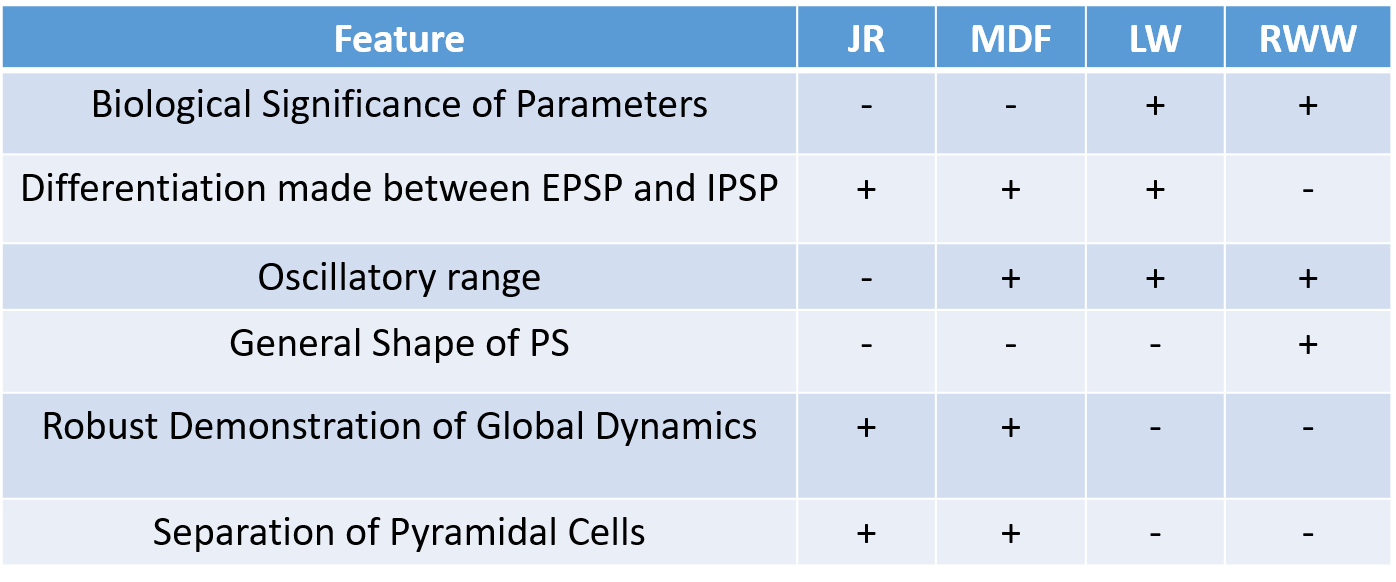
\includegraphics[scale=0.5]{Images/Table_global_eval.png}
   % \caption*{\textbf{Table.  \textit{Global evaluation of the models}} More details need to be given}   
   % \label{fig:Global_eval}
%\end{figure}



\begin{table}[]
    \rowcolors{2}{gray!20}{gray!70!}
    \centering
    \begin{tabular}{ccccc}
        \rowcolor{black} 
        \textcolor{white}{Feature} & \textcolor{white}{JR} & \textcolor{white}{MDF} & \textcolor{white}{LW} & \textcolor{white}{RRW} \\
        \hline
        Biological significance of Parameters & - & - & + & + \\
        Differentiation between EPSP and IPSP & + & + & + & - \\
        Oscillatory range & - & + & + & + \\
        General shape of PS & - & - & - & + \\
        Robust Demonstration of Global Dynamics & + & + & - & - \\
        Separation of Pyramidal Cells & + & + & - & -
    \end{tabular}
    \caption*{\textbf{Table 3. \textit{Global evaluation of the models.}} Different features of the models are assessed, highlighting strengths and limitations. In terms of robustness and tractability, the JR and MDF models prove more suitable. The LW model incorporates more physiological elements, and the RRW model shows a stronger capability in reproducing empirical features of alpha activity.} 
    \label{tab:global_eval}
\end{table}


%\subsection{Other types of models/Non-Neural Population models of the Alpha Rhythm}
\subsection{Alternative models of alpha rhythm beyond NPMs}
%Note: Title will depend if talk about conductance-based models as well or not
% Other types of alpha models or other types of mesoscopic scale models. Review on EEG models: https://link.springer.com/article/10.1007/s10548-021-00828-2

In this paper we have elaborated on a select few NPMs that specifically address alpha oscillations, following the corticocortical or corticothalamic alpha theory candidates summarized in Fig. 2. It is also important to note however that alpha rhythms have been studied by researchers at a variety of scales using models ranging from microscopic to macroscopic perspectives. Many of these extend beyond the scope of the present work due to being either not (mesoscale) NPMs, or not corresponding to the corticocortical/corticothalamic theory types. In this final section we review briefly a selection of this broader body of work developing alternative alpha rhythm and related computational models.
% Include deco and jirsa 2012 used by sciencedirect.com/science/article/pii/S1053811913011014#bb0140
%1) other NPM: conductance-based NMM,  activity-based (WC)\\


\subsubsection{Two levels down:  multicompartmental microcircuit models}
Multicompartmental models are the most established `low-level' description of single-neuron structure and dynamics, aiming to replicate as faithfully as possible their morphological characteristics, membrane biophysics, and synaptic kinetics within the mathematical framework of equivalent electrical circuits. In multicompartmental models, the activity of the neurons are described with the Hodgkin-Huxley equations. This approach can capture the complex electrical signaling that occurs within neurons and can provide a more accurate representation of how neurons interact with one another in neural circuits. Mesoscale dynamical phenomena such as oscillations are usually studied with this approach as emergent properties of networks containing hundreds or thousands of multicompartmental neurons, designed according to known architectural features of specific brain structures such as cortex \citep{hay2011models}, thalamus \citep{iavarone2023thalamic}, or hippocampus \citep{chatzikalymniou2021linking}. Interestingly, despite the prominence of this general modelling paradigm in computational neuroscience, there are (to our knowledge) no established and/or consistently explored models of multicompartmental circuit models of EEG alpha. 

%somatomotor analogue occmu rhythm - generate the mu-rhythm composed of alpha and beta rhythms observed in the primary somatosensory cortex to explain the neural origin of spontaneous rhythms. 

An influential line of work in this area was first introduced by \citet{jones2009quantitative}, and continued more recently \citep{neymotin2020human,studenova2022non}. These authors used a multicompartmental circuit model to simulate the $\mu$ rhythm, the somatosensory analogue of occipital alpha. The extent to which this model constitutes a `true' alpha rhythm model is unclear, however, since a major component of the circuit described in \citet{jones2009quantitative} is a pacemaker-like 10Hz thalamic drive. More recently, Hay and colleagues developed a detailed columnar microcircuit model (L2/3), based closely on newly-characterized morphological and electrophysiological properties of human cortical tissue, which has been shown to generate resting state EEG features such as the alpha rhythm \citep{yao2022reduced, mazza2022eeg}. Specifically, the model was used to investigate the effects of reduced cortical inhibition by somatostatin-expressing (SST) interneurons, a key element in the altered inhibition observed in treatment-resistant major depressive disorder. Comparing simulated healthy resting state EEG with depressed EEG (characterized by reduced SST) revealed significant changes in EEG. This discovery provides biomarkers that establish a connection between interneuron inhibition levels and quantifiable EEG patterns, thereby facilitating the identification of depression subtypes and the noninvasive monitoring of cortical inhibition modulation.

%It may be used to investigate cellular mechanisms involved in oscillatory generations.\\ 
%Some other examples of popular multi-compartmental models include the NEURON simulator, the GENESIS simulator, and the BlueBrain simulator. Overall, multi-compartmental models have proven to be a valuable tool for studying the complex biophysics of neurons and neural circuits.
%Their team developed the \textit{Human Neocortical Solver (HNN)}, a user-friendly software tool to simulate neocortical circuits, in order to interpret human EEG/MEG recordings at the level of circuit activity and cellular mechanisms \citep{neymotin2020human}. 


\subsubsection{One level down: spiking neuron network models}
Whilst the individual elements in morphologically detailed circuit models such as those reviewed above are able to capture most of the known physiological properties of single neurons, they are potentially a suboptimal level of description for modelling oscillatory neuron behaviour that occurs due to (micro-scale) network organization. Spiking neuron models, which aim to capture accurately the membrane potential and firing dynamics of individual cells, but not their extended spatial structure, are the most commonly employed level of description in computational neuroscience for purely network-based activity patterns. 

One notable example of this was described in the seminal paper of \citet{izhikevich2003simple}, where the influential phenomenological single-neuron model was introduced, that is able to accurately reproduces neuronal spiking dynamics without the full complement of Hodgkin-Huxley ionic currents \citep{izhikevich2003simple}. By simulating a network of 1000 randomly spiking neurons of this kind, alpha and gamma rhythms could also be generated. Subsequently, this model was used as the basic component of a large-scale representation of the mammalian thalamocortical system, which featured 22 neuronal cell types, six-layered cortical microcircuits, multiple thalamic nuclei, and white matter connectivity informed by diffusion-weighted MRI tractography \citep{izhikevich2008large}. From their simulations with this model, the authors suggest that variations in rhythmic frequencies across different brain regions may arise from differences in white matter connectivity between and among cortical areas. 


%make sure say integrate and fire model

%have shown the ability to self-organize in order to generate collective frequency rhythms including delta, alpha and gamma oscillations. 
%Compared to NPMs, they incorporate much greater biological details enhancing their physiological relevance and predictive capabilities. Models of spiking networks have shown the ability to self-organize in order to generate collective frequency rhythms including delta, alpha and gamma oscillations. 
%At the individual neuron level, models have been developed to describe neural activity at the microscopic scale and to capture the complex oscillatory patterns observed in neural systems. 
%Spiking neural networks, for example, simulate thousands of spiking neurons exhibiting bursting activity and randomly coupled synapses. 
%The purpose of those models is to gain an understanding of the role of cell types and connectivities. Compared to NPMs, they incorporate much greater biological details enhancing their physiological relevance and predictive capabilities. Models of spiking networks have shown the ability to self-organize in order to generate collective frequency rhythms including delta, alpha and gamma oscillations. 

%However, in addition to being tremendously computationally intensive, it is unclear whether spiking neural models can offer meaningful interpretations of empirical data on large-scale brain activity. 


\subsubsection{One level up: whole-brain NPMs}

The large-scale spiking neuron model of \citep{izhikevich2008large} is an interesting early example of whole-brain modelling \cite{griffiths2022whole}, a sub-field of computational neuroscience that emerged in the mid 2000s, drawing strongly on developments in neuroimaging connectomics.

Whilst spiking network models have been employed with varying levels of anatomical precision in whole-brain modelling studies \citep{deco2013resting, pronold2023multi}, they have not been used extensively to study alpha rhythms specifically. Rather, whole-brain models of EEG alpha activity have for the most part used NPMs, of the kind discussed extensively in the present work \citep{stefanovski2019linking, griffiths2020connectome, abeysuriya2018biophysical}. The essential level of description in this case, notwithstanding some properties that result from large-scale network interactions and delays, for the most part the key level of analysis for understanding whole-brain networks of coupled NPMs is in fact individual NPM units themselves. From this point of view, the survey presented in the present work is of fundamental relevance to whole-brain alpha NPM models. Even though we have not explored here the question of how NPMs behave when coupled together into networks. The interesting case where this heuristic does not apply is when the alpha-generating mechanism in a whole-brain model occurs at the network level, and not at the level of individual nodes or NPM units. 

The motivating argument here, which applies equally to whole-brain vs. single-node NPMs and to microcircuit network vs. single-cell models, is that the emergent properties of interconnected neuronal ensembles may be unrelated to the activity of individual neurons \citep{raj2020spectral}. The extensive complexity introduced by numerous equations and parameters in more complex models can in this case become a `black box', limiting the ability to draw conclusions on the core network-level rhythmogenic mechanisms \citep{taher2021next, turker2005black}.

%Th is approach suggests that long-range structural connectivity is the key to regulating brain activity, rather than the local activity of individual neurons. \citep{abdelnour2014network, destexhe2009wilson, robinson2005multiscale}. 

An important new line of research motivated by these considerations is the spectral graph theory framework proposed by \citet{raj2020spectral}. These authors introduced a hierarchical, linear, analytic spectral graph model capable of replicating empirical MEG spectra and the spatial distribution of alpha and beta frequency bands \citep{raj2020spectral}. Compared to BNMs and NFMs, the advantage of this type of modelling lies in providing steady-state frequency responses obtained from the eigendecomposition of a graph Laplacian, offering a closed-form solution of brain oscillations \citep{verma2022spectral}. This makes them computationally efficient and less time-consuming. However, a major limitation is the lack of clear biological interpretability in the local parameters and gain terms of simpler spectral graph models. A more recent modified spectral graph model by Verma et al. revisited Raj et al.'s work using a bottom-up approach to make it more biophysically relatable at the local scale while still capable of representing the same spatial patterns as the original model \citep{verma2022spectral}. Despite this improvement, spectral graph models may not be ultimately suitable for capturing the full range of dynamical solutions, which could be effectively addressed by nonlinear BNMs \citep{verma2022spectral}. 

%Spectral graph theory modelling presents a promising avenue for studying brain-wide neural activity, but it is important to carefully consider its limitations and potential applications in specific research contexts.

%- Resting state networks: \citep{deco2011emerging}

%MAYBE PUT THIS SECTION IN LIMITATIONS

%\subsubsection*{
%\textit{Next generation neural mass models}}

%As mentioned in the limitations, NMMs assume that neurons within a population are synchronized and thus are unable to reproduce event-related desynchronisation (ERD), and the latter event-related synchronisation (ERS) at the single population level which Coombes et al. try to address with this next generation of NMM \citep{coombes2019next}. They present a $\theta$-neuron model, which has been shown to have an exact mean-field description for instantaneous pulsatile interactions. By incorporating a more realistic synapse model, the mean-field model is extended to include many of the features of a neural mass model, as well as a further dynamical equation that describes the network synchrony evolution.

% Add Gast Knoshe 2020 2021 montbrio model 
%- Whole-brain level (macroscopic). Study concurrently with connectivity and fMRI data, talk about NPM at whole brain scale

%Gast et al. describe bursting dynamics in spiking neural networks with short-term adaptation using a mean-field approach. Although NMMs are appropriate for studying the emergence of bursting behavior in coupled neural populations, they are of a phenomenological nature and do not provide a clear mechanistic link to the underlying spiking neurons. Therefore, they offer limited insight into the emergence of bursting solely based on a population's intrinsic dynamics. They try to  bridge the gap between the exploration of bursting in spiking neural networks and NMMs.

%All these other methods have their own advantages and limitations and the choice of a modelling approach highly depends on the specific research objective. Since we are interested in understanding underlying physiological processes observed at the level of the EEG, NPMs integrated in a whole-brain model seem an adequate fit and have new platforms being developed such as the Virtual Brain. NPM have been predominantly useful to understand brain rhythms since the 1970's. 
%
%Interesting source for different types of models: `Which model to use for cortical spiking neurons?'
%\begin{figure}[H]
%    \centering
%    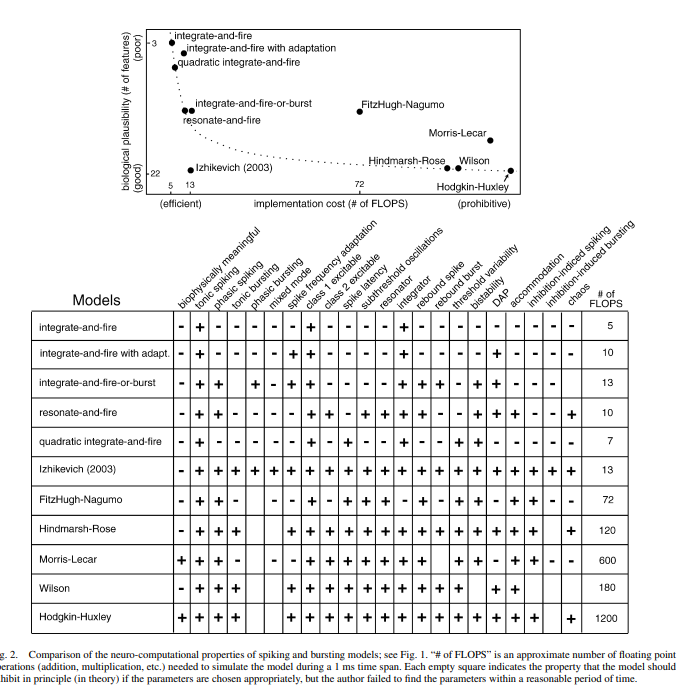
\includegraphics[scale=1]{Images/Model_Comparison.png}
%    \caption*{\textbf{Figure 23.  \textit{Taken from Iziekvitch 2004, %comparison between models.}} Add more description... }     
%    \label{fig:comparison}
%\end{figure}
%
%
%NOTE: Do we want a section mentioning models replications abnormal alpha oscillations related to a disease? (e.g. Battacharya model)\\
%
%\subsection{Future Work or conclusion on the two theories}

%\subsection{Summary}
\subsection{Conclusion and future work}

% left this here as a maybe...
% is also still in the text block at the start of this chapter
In conclusion, our comparative analysis of the JR, MDF, LW, and RRW models elucidate the relationship between their mathematical formulations and parameters, and providing a range of biological insights. Our novel simulations with these models showed differing levels of precision in replicating EEG alpha characteristics, demonstrating how their dynamical behavior is impacted by rate constants and connectivity parameters.

Future computational studies of alpha rhythmogenesis in human EEG should include investigations of intracortical and corticothalamic models at the scale of the whole brain. This is particularly important since, as we have discussed, mesoscale empirical data at the level of single neural populations alone, which has been our focus in this paper, may be insufficient to distinguish between these two theories. A key objective of these investigations should be to determine conclusively whether the contribution of the thalamus is essential for the generation of resting state alpha oscillations. We hypothesize that topographic variation in oscillatory brain activity, as well as network-level connectivity and dynamics, will provide important additional information for this objective. Furthermore, at the whole-brain level, each node is part of a larger network, and so the dynamics of the neural populations studied in the present work may be modified substantially when interconnected via the connectome. Finally, improving validation methods against empirical data, for example by extending the number and type of EEG features used for model comparison and fitting, would allow for better differentiation between models and determination of which ones are more accurate representations of observed brain dynamics.





%PREVIOUS SUMMARY AND CONCLUSION
%Throughout this review, four prominent intracortical and cortocothhalamic models are discussed and compared in depth to provide an explicit investigation of alpha rhythm NPM and determine the dynamics and alpha mechanisms represented with each of them. A goal was to assess whether this analysis would shed some light on the two proposed theories while providing a synthesis of the two theoretical formulation of alpha together. After laying out the mathematical expressions, the simulation results obtained with standard parameter values are first investigated followed by extension of the parameter space to identify the necessary conditions to produce alpha rhythms as well as the influence of parameters with a focus on rate constant and E-I connectivity strength. Finally, a general comparative evaluation of the models establishing commonalities and differences between them is given.
%The investigation revealed that even though the models represent different neural population or topologies at the core these models are very similar. For example, all of the models are capable of simulating resting-state alpha with characteristic features found in empirical EEG data some with more accuracy than others. Therefore, at this level it seems difficult to ascertain if integrating the thalamus is required for the generation of resting-state occipital alpha or if any E-I interaction including intracortical is sufficient to generate posterior alpha. From the E-I investigation, within certain frequency ranges, the models have similar E-I behavior. For all the models, the gain of the E-I loop affects the dynamics observed and thus the neural activity. With the LW model, it seems that changes in the number and strength of GABA interneurons synapses are more likely to affect the dynamics. Further investigation of the stability of the JR and LW models, revealed that the standard alpha oscillation generated by each of them stems from a different mechanisms: limit-cycle or noise-driven. 
%With the intrathalamic E-I loop, the gain also affects the general dynamics and even though there is a slight shift in the central frequency, the main role of the intrathalamic loop seems to modulate the magnitude of the peak. 
%In summary, by exploring the connectivity parameter spaces, we identified different alpha mechanism between JR and LW, and for RRW, the intrathalamic loop tended to modulate the alpha peak allowing us to define various alpha dynamics throughout the space and the role of the E-I in each model. 
%Furthermore, variations in rate constant lead to different dominant frequency of oscillation with higher values leading to stronger delays and thus a decrease in the frequency of oscillation. 

%By evaluating the models at this scale and assessing the similar and different dynamics, it is inconclusive whether one theory is more likely than the other. Selecting a model compared to another one will dependent on the goal of the study. 
%Nonetheless, specific features of the EEG tended to be better represented by certain model. For instance, the 1/f scaling is better captured with the RRW model, indicating that if you wish to study differences in this slope (such as in stroke patient), this model would be more suitable.  


%\subsection{Concluding Remarks and Future Work}

%A central purpose of the paper was to compare existing popular intracortical and corticothalamic NPM that we deemed encompassing the different formulations and advanced research on the understanding of alpha rhythmogenesis. 
%The scope of our study is biologically inspired phenomenological models with a focus on rate constant and E-I connectivity parameters for a meaningful evaluation. 

%Validation of NPM against empirical data is a challenging task as of today it is mostly based on the visualization of EEG data representing the macroscale. Variables used at the mesoscopic scale do not have thorough empirical bases to compare against. Therefore, distinction between the models presented on an assessment against EEG data and relies on parameter space searches to identify general trends. Throughout this work, since similar behavior was identified namely in their E-I interactions, it is difficult to affirm confidently which one is better represent alpha oscillations and thus which theory is more plausible. However, each model have their respective advantages and limitations which will define their use cases. Choosing a model over another will depend on their capacity to represent certain features or the inclusion of more biological details. 
%However, at this scale, we were able to identify the role of the E-I loop in each model and how the gain will influence the dynamics represented as well as various alpha mechanisms. Biologically, shows how imbalance in E-I can lead to altered dynamics (either different oscillatory patterns or reduce alpha magnitude). 
%Future work on gaining insight into alpha rhythmogenesis, includes investigating intracortical and corticothalamic model at the scale of the whole-brain as the mesoscopic scale empirical data is insufficient to validate a theory over another one. The aim would be to determine if the contribution of the thalamus is essential for the generation of resting-state alpha oscillation. We hypothesis that the network connectivity will bring additional information and would allow us to differentiate between the two theories. Furthermore, the node is part of a network and the dynamics will likely be affected by the connectome. NPMs require an improvement of the validation methods against empirical data to allow for better differentiation between the models and define which are more realistically accurate.
%On the modelling perspective, future work could include a similar comparison analysis with conductance-based models focused on alpha oscillations. 

%\section{Data and Code Availability}
%All related files and programming code are publicly available on GitHub at \url{https://github.com/GriffithsLab/Bastiaens2024_AlphaModels}

%\section{Author Contributions}
%SB: conceptualization, methodology, formal analysis, writing—original draft, writing—review and editing, and visualization. JG: conceptualization, methodology, writing—review and editing, supervision, and funding acquisition. DM: writing—review and editing, visualization.

%\section{Funding}
%This work was supported by the Krembil Foundation (to JDG), the Labatt Family Network (to JDG), the CAMH Discovery Fund (to JDG) ,and the Canadian Institutes of Health Research Grant (to JDG). 

%(The funders had no role in study design, data collection and analysis, decision to publish, or preparation of the manuscript.)

%\section{Declaration of Competing Interests}
%The authors have declared that no competing interests exist.


\bibliography{references}


\newpage
%TC:ignore
\section*{Supplementary Information}

In the following, we provide additional information on various technical details and additional analyses from our study, which were not included in the main text primarily due to space reasons. These pages cover the derivation of the JR model differential equations (Section S1), the comparison of connectivity parameter spaces between JR and MDF (Section S2), the phase plane analysis of JR (Section S3), the reduced 3D parameter space of MDF (Section S4), the 4D JR connectivity analyses (Section S5), and finally, the full model equations with a description of their parameters and standard alpha values (Section S6).
Note that complete code for the generating figures in the following and in the main text is openly available at \url{github.com/griffithslab/Bastiaens2024_AlpaModels}.


\newpage
\subsection*{S.1 Derivation of the JR Model Equations}

The Jansen-Rit and related models are often discussed in terms of a convolution integral for the synaptic impulse response function, as well as the corresponding equivalent second-order differential equation, which is typically what is actually used in numerical simulations. The mathematical relationship between these is however rarely given in literature sources, and so we provide that here, with a full derivation of the JR differential equation from its impulse response, using the Laplace transform as it simplifies convolution operations by turning them into algebraic manipulations in the Laplace domain.

The synaptic impulse response is defined as an alpha function, which is described by the following equations:
\begin{equation}\label{my_first_eqn}
	h(t) =     
	\begin{cases}
      \alpha \beta t e^{-\beta t}, & t \geq 0\\
      0 & \text{otherwise}
    \end{cases}
\end{equation}
with $\alpha$ as the maximum amplitude of the PSP and $\beta$ the rate constant parameter. The first step consists of finding the Laplace transform of $h(t)$, denoted as $H(s)$, which is defined as follows:
\begin{eqnarray}
    H(s) = \mathcal{L}\{h(t)\} &=& \int_{0}^{\infty} h(t)e^{-st} \,dt \\
    &=& \int_{0}^{\infty} \alpha \beta t e^{-\beta t}e^{-st} \,dt \\
    &=& \int_{0}^{\infty} \alpha \beta t e^{(-\beta-s) t} \,dt \\
    &=& \lim_{b\to\infty} \left[ \int_{0}^{b} \alpha \beta t e^{(-\beta-s) t} \,dt\right]\\
    &=& \lim_{b\to\infty} \left(\left[ \alpha \beta t \frac{1}{-\beta -s}e^{(-\beta-s) t} \right]_0^b - \int_{0}^{b} \frac{\alpha \beta}{-\beta-s}e^{(-\beta-s) t}\,dt\right)\\
    &=& \frac{\alpha \beta}{-\beta -s}\lim_{b\to\infty}\left(be^{(-\beta -s)b}- \int_{0}^{b} e^{(-\beta-s) t}\,dt\right)\\
    &=&\frac{\alpha \beta}{\beta + s}\lim_{b\to\infty} \int_{0}^{b}e^{(-\beta -s)t}\,dt\\
    &=&\frac{\alpha \beta}{\beta + s}\lim_{b\to\infty} \left[ \frac{1}{-\beta -s}e^{(-\beta-s) t} \right]_0^b\\
    &=&\frac{\alpha \beta}{(\beta + s)^{2}}\lim_{b\to\infty} \left[1 - e^{(-\beta -s)b} \right]\\
    &=& \frac{\alpha \beta}{(\beta + s)^{2}}
\end{eqnarray}

Now, with an expression for $H(s)$ in the Laplace domain, and given that $y(t)$ is equal to the convolution of $h(t)$ and $x(t)$, we can represent this relationship in the Laplace domain as:
\begin{eqnarray}
    Y(s) &=& X(s)H(s)\\
    Y(s) &=& X(s)\frac{\alpha \beta}{(\beta + s)^{2}}\\
    (\beta +s)^{2}Y(s) &=& X(s)\alpha \beta\\
    s^{2}Y(s) + \beta^{2}Y(s) + 2\beta s Y(s) &=& \alpha \beta X(s)\\
    s^{2}Y(s) &=& \alpha \beta X(s) - 2\beta s Y(s) - \beta^{2}Y(s)
\end{eqnarray}
Since $s^{2}Y(s)$ corresponds to the second derivative in the time domain, translating equation (40) back into the time domain, we obtain:
\begin{equation}
    \ddot{y}(t) = \alpha \beta x(t) - 2\beta \dot{y}(t) - \beta^{2}y(t)
\end{equation}
This corresponds to the commonly used Jansen and Rit second-order differential equation, which can be rewritten in the form of two first-order ODE's:
\begin{eqnarray}
    \dot{y}(t) &=& z(t)\\
    \dot{z}(t) &=& \alpha \beta x(t) -2\beta z(t) - \beta^{2}y(t)
\end{eqnarray}
with $y(t)$ representing the average postsynaptic membrane potential (output of the PSP block). 

\newpage
\subsection*{S.2 Comparison of MDF and JR connectivity parameter spaces }

By setting the parameters to be the same between JR and MDF, we compare the connectivity parameter space of the two models (Fig. S1).
%The effect of the connectivity parameters on the MDF model was explored. Similarly to JR, we have $\gamma_{1}$, $\gamma_{2}$, $\gamma_{3}$ and $\gamma_{4}$. We defined the connectivity parameter space for different values of $\gamma_{5}$ corresponding to the self-inhibitory connection. 

%The general shape of the heatmaps is comparable to JR with the difference that for the same combination of values, the model tends to produce oscillation of higher frequencies in the beta range. 


%1) Different combinations of $\gamma_{5}$
%\begin{figure}[H]
 %   \hspace{-1.5cm}
  %  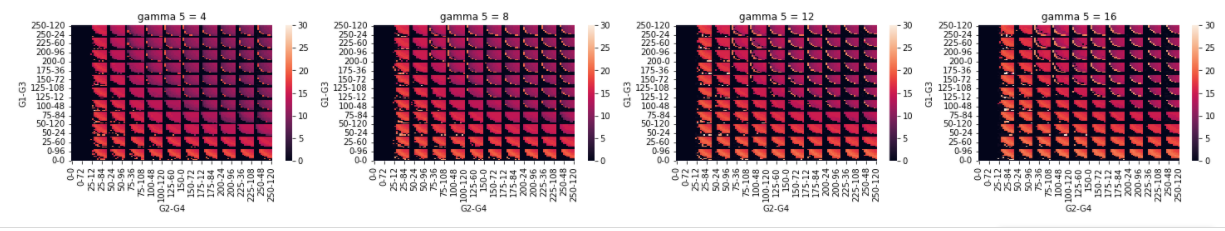
\includegraphics[scale=0.6]{Images/Moran_Connection_2.png}
   % \caption*{\textbf{Figure 19.  \textit{Connection strength parameter space for MDF for different values of $\gamma_{5}$. The maximum frequency is set 30mV for visualization purposes.}} From left to right: $\gamma_{5}$ =4; $\gamma_{5}$ = 8; $\gamma_{5}$ = 12; $\gamma_{5}$ = 16. Outer axes:$\gamma_{1}$ and $\gamma_{2}$; Inner axes: $\gamma_{3}$ and $\gamma_{4}$ Rhythms generated tend to slightly increase with increase $\gamma_{5}$ values.}    
   % \label{fig:MO_gamma}
%\end{figure}

%2) Focus on $\gamma_{5}=16$

%\begin{figure}[H]
    %\hspace{-1.5cm}
    %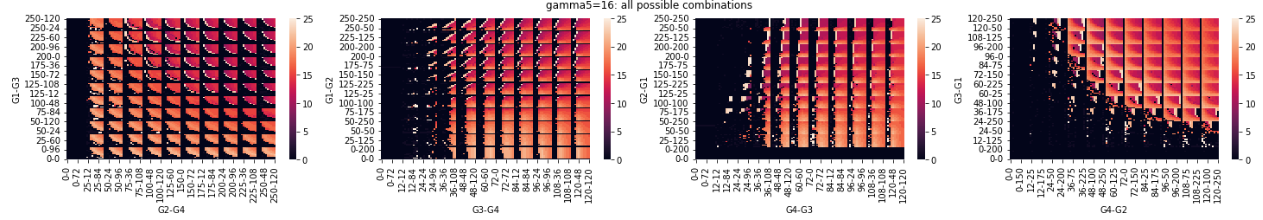
\includegraphics[scale=0.6]{Images/MR_All_Config_vmax_25.png}
  %  \caption*{\textbf{Figure 20.  \textit{Connection strength parameter space for MDF in different combinations with $\gamma_{5}$. Maximum frequency is set at 30mV.}} From Left to Right: 1) Outer axes $\gamma_{1}$-$\gamma_{2}$; Inner axes $\gamma_{3}$-$\gamma_{4}$; 2) Outer axes $\gamma_{1}$-$\gamma_{3}$; Inner axes $\gamma_{2}$-$\gamma_{4}$; 3)  Outer axes $\gamma_{2}$-$\gamma_{3}$; Inner axes $\gamma_{1}$-$\gamma_{3}$; 4) Outer axes $\gamma_{3}$-$\gamma_{4}$; Inner axes $\gamma_{1}$-$\gamma_{2}$}     
  %  \label{fig:MO_gamma16}
%\end{figure}

%Even though not exactly same, point is to show what new connection brings and if in general get similar effect than Jansen (similar trends)

\begin{figure}[H]
    \centering
    %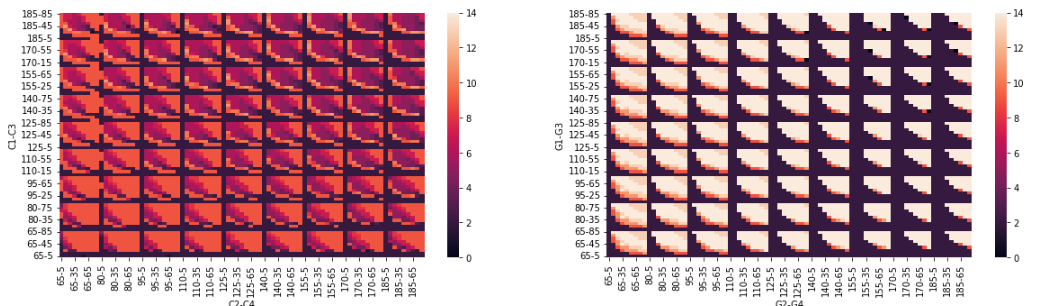
\includegraphics[scale=0.5]{Images/Comp_JR_MR_with_gamma_5.png}
    %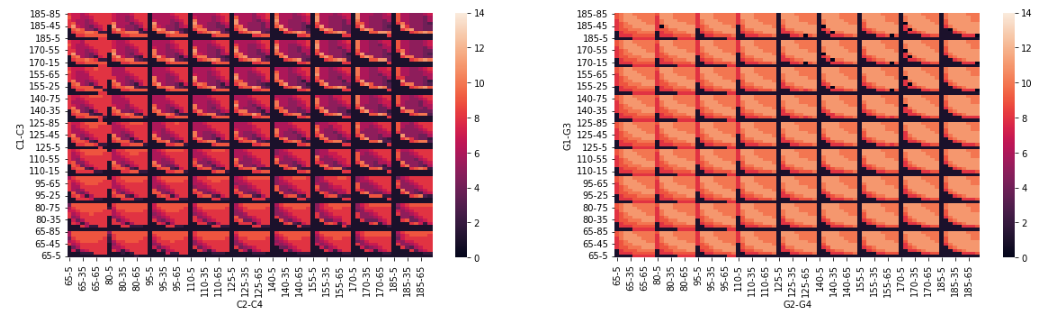
\includegraphics[scale=0.5]{Images/Comp_JR_MR_without_gamma_5.png}
    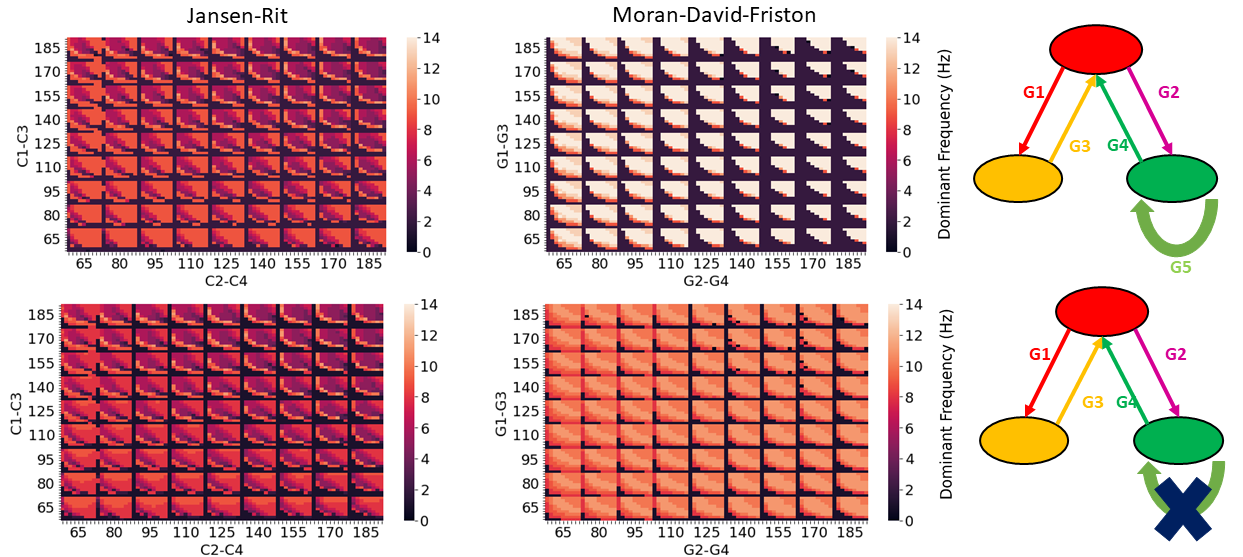
\includegraphics[scale=0.5]{Images/MDF_Appendix.png}
    \caption*{\textbf{Figure S1.  \textit{Connection strength parameter spaces for JR and MDF with similar parameter settings.}} In the top, for MDF $\gamma_{5} = 16$, and at the bottom $\gamma_{5} = 0$. The general shape of the dynamics is very similar between the two, suggesting that the effects of connectivity are the same. However, MDF tends to generate oscillations of higher frequencies for identical connectivity parameter sets, even when the $\gamma_{5}$ connection is removed.}     
    \label{fig:LI_CS}
\end{figure}

In the top row of Fig. S1, we compare JR against MDF with the self-inhibitory connection. We observe a similar triangular boundary shape within which the system oscillates. However, MDF tends oscillate at higher frequency that exceed the alpha range (Fig. S1, MDF top row, colors are brighter than JR). When the self-inhibitory connection is removed in MDF (Fig. S1, MDF bottom row), the system now oscillates at the alpha frequency. It does not present lower frequencies, such as those in the JR model where we have slower oscillations. Thus, MDF seems to oscillate at higher frequencies than JR. Nonetheless, we observe that the two models share this similar triangular shape with non-oscillatory behavior when $C_3$ and $C_4$ are too low, suggesting similar global dynamics. The main conclusion drawn from this analysis is that the self-inhibitory connection introduced in MDF grants the model the ability to generate oscillations at a higher frequency than alpha, a more challenging capability compared to JR. 


\newpage
\subsection*{S.3 Phase plane of JR in 3D}

For the stability analyses in Fig. 12, we have only presented the phase plane with the pyramidal and inhibitory population output voltages. Considering the trajectory of the third excitatory neural population activity alongside these can provide a better understanding of the full picture however, as can be seen in Fig. S2.


\begin{figure}[H]
    \centering
    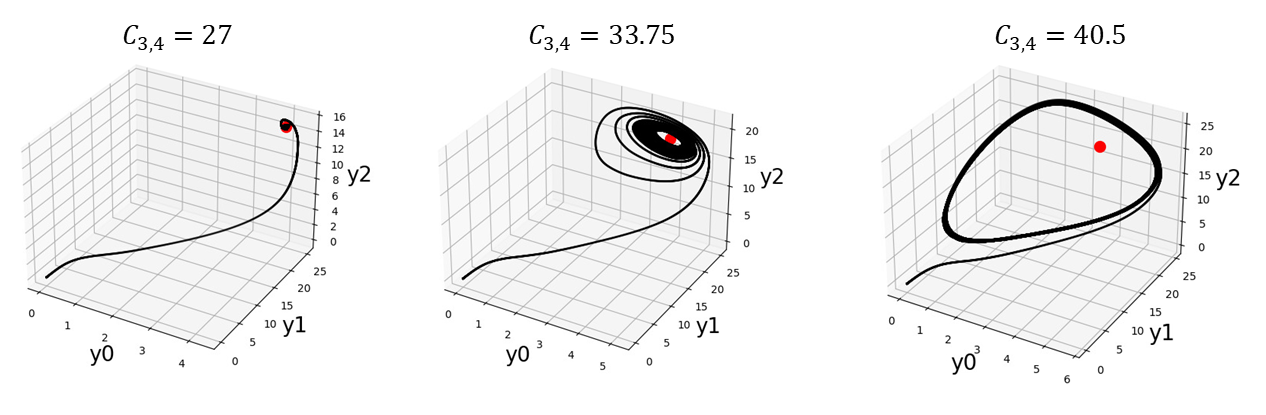
\includegraphics[scale=0.5]{Images/Appendix_stab.png}
    \caption*{\textbf{Figure S2.  \textit{Phase plane of JR for different E-I connectivity parameters.}} The trajectory of the three neural populations (with $y_0$, $y_1$, and $y_2$ corresponding to the output of the PSP block for the pyramidal cells, excitatory interneurons, and inhibitory interneurons, respectively) can be inferred by examining the stability of their respective fixed point (red). When $C_{3,4} = 27$, the fixed point is stable and no oscillations occur. For $C_{3,4} = 33.5$, the system enters a limit cycle with the oscillation frequency of alpha. Finally, when $C_{3,4} = 40.5$, the limit cycle widens and the frequency of oscillation is reduced.}     
    \label{fig:Stability3D}
\end{figure}

As seen in our previous phase plane analysis, for specific connectivity parameters, the system either reaches a fixed point or enters a limit cycle defining the frequency of oscillation. The results closely resemble those in Fig. 12, 1b, implying that the dynamics primarily involve interactions between the pyramidal and inhibitory populations, with minimal contribution from the third population in this case.

\newpage
\subsection*{S.4 3D parameter space with MDF}

We simplified the 5-dimensional connection parameter space into a 3-dimensional representation for the MDF model, using its linearized version. Stability is assessed by looking at the system's poles within the transfer function of the system.
The aim was to establish a parallel with the 3D `xyz' corticocortical/corticothalamic/intrathalamic lumped gains reduced parameter space discussed in a number of studies using the RRW model (although for reasons of space we have not focused on that aspect of RRW in the present paper \citealp{robinson2002dynamics,robinson2005multiscale, roberts2012corticothalamic, breakspear2006unifying, abeysuriya2015physiologically}), and determine the effects of the loops on the dynamics of the MDF model.
%The result is similar to the 3D  `xyz' corticocortical/corticothalamic/intrathalamic lumped gains reduced parameter space discussed in a number of studies using the RRW model (although for reasons of space we have not focused on that aspect of RRW in the present paper). 
%(Do I explain I rewrote the transfer function another way with numerator and denominator instead of matrix form as in the paper?)

\begin{figure}[H]
    \centering
    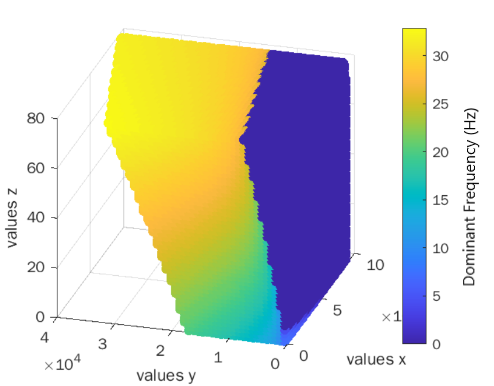
\includegraphics[scale=0.6]{Images/3dmoran1.png}
    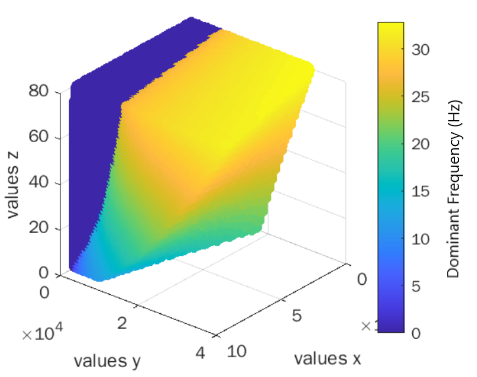
\includegraphics[scale=0.6]{Images/3dmoran2.png}
    \caption*{\textbf{Figure S3.  \textit{Visualization of dynamical regimes of the MDF model in a 3D setting using the linearized expression.}} The x-axis corresponds to effect of the excitatory loop ($\gamma_{1}*\gamma_{2}$); the y-axis represents the effect of the inhibitory loop ($\gamma_{3}*\gamma_{4}$); and the z-axis is the effect of the self-inhibitory loop ($\gamma_{5}$). As $\gamma_{5}$ values increase, the system tends to oscillate at a higher frequency.}
    \label{fig:3D_Moran}
\end{figure}

The aim here is to easily visualize the regions of stability and dynamics as a function of the `loops', rather than a single connectivity parameter. As expected, with the increase in the self-inhibitory connection (z-axis), the dominant frequency of oscillation gradually shifts from theta to alpha and then to the beta range.


\newpage
\subsection*{S.5 4D JR connectivity analysis}

In the JR model, our focus was specifically on $C_{3}$ ($P \rightarrow I$) and $C_{4}$ ($I \rightarrow P$) as the E-I loop, but there is also the interaction between excitatory interneurons and pyramidal cells ($C_{1}$ ($P \rightarrow E$) and $C_{2}$ ($E \rightarrow P$)) to consider. Typically, the ratio between these values is varied. By simulating time series for different values of $C$ with the standard ratio values ($C_{1}=C$, $C_{2}=0.8*C$, $C_{3}=0.25*C$ and $C_{4}=0.25*C$), we can infer that increasing values of C lead to a decrease in the frequency of oscillation up to a certain point (Fig. S4), which concurs with results from \citet{jansen1995electroencephalogram}. \\

\begin{figure}[H]
    \centering
    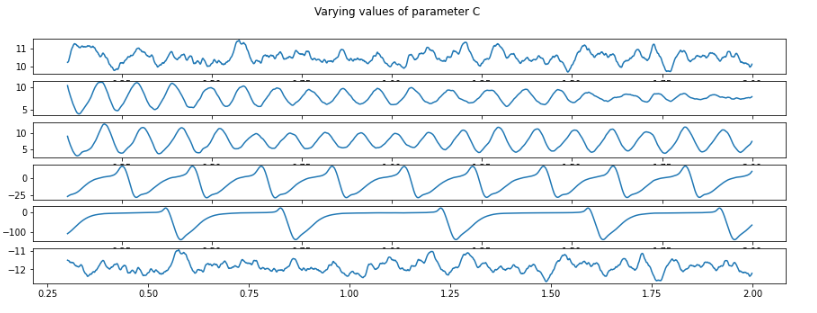
\includegraphics[scale=0.75]{Images/JR_Varying_C_time_series.png}
    \caption*{\textbf{Figure S4.  \textit{Simulated time series of JR for different connectivity C values.}} From top to bottom: $C= 68$, $C=128$, $C=135$, $C=270$, $C=675$, $C=1350$. As connectivity values increase, the frequency of oscillations decreases up to $C=675$.}    
    \label{fig:JR_Ctime}
\end{figure}

Changes in the frequency of oscillation as a function of connectivity ratios are presented in the form of 4D heatmaps in a 2D space (Fig. S5). The general trend observed is that higher connectivity values result in slower oscillations, as expected. 



\begin{figure}[H]
    \hspace{-1cm}
    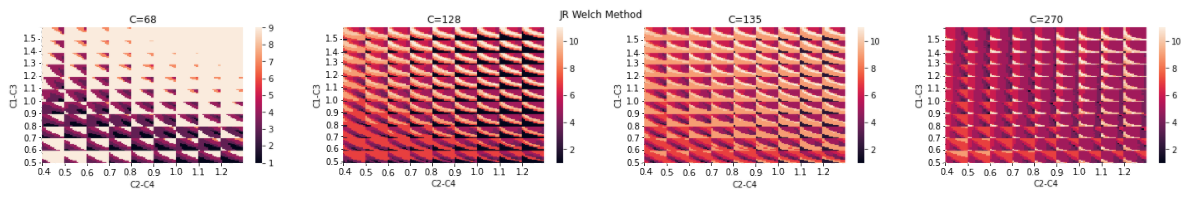
\includegraphics[scale=0.60]{Images/JR_Connection_2png_new.png}
    \caption*{\textbf{Figure S5.  \textit{Variation in  the frequency of oscillation as a function of connection strength for JR for different $C$ values.}} From left to right: $C=68$, $C=128$, $C=135$ and $C=270$. The outer axes $C_{1}-C_{2}$ represent the excitatory loop, while the inner axes $C_{3}-C_{4}$ represent the inhibitory loop. The results correlate with what is observed in the time series. The parameter space is obtained by changing the ratio of each connection (i.e: $C1 = 0.8$ corresponds to $C1 = 0.8*C$)}       
    \label{fig:JR_Cconnection}
\end{figure}

To observe the different trends that emerge, we focused on the case where $C$ equals 135 and investigated the different possible combinations of parameters on the outer and inner axes (Fig. S6).

\begin{figure}[H]
    \hspace{-1.3cm}
    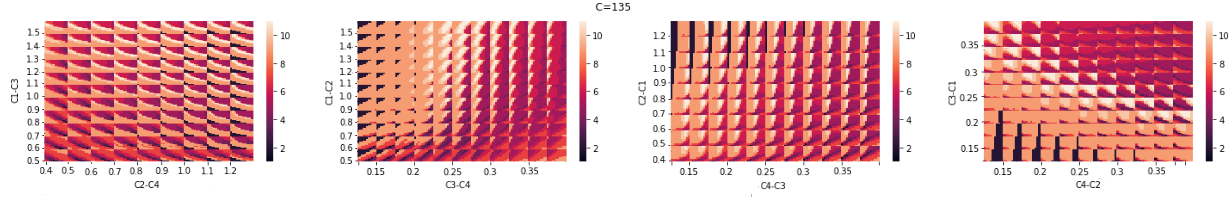
\includegraphics[scale=0.58]{Images/JR_All_Config_new.png}
    \caption*{\textbf{Figure S6.  \textit{Connection strength parameter spaces for Jansen-Rit in different combinations with C=135.}} Each combination reveals a distinct pattern, aiding in visualizing the relationships among all the connectivity parameters. From left to tight: 1) Outer axes $C_{1}-C_{2}$ Inner axes $C_{3}-C_{4}$; 2) Outer axes $C_{1}-C_{3}$; Inner axes $C_{2}-C_{4}$; 3)  Outer axes $C_{2}-C_{3}$; Inner axes $C_{1}-C_{3}$; 4) Outer axes $C_{3}-C_{4}$; Inner axes $C_{1}-C_{2}$}            
    \label{fig:JR_C135}
\end{figure}

Clear patterns emerge in two different cases. When $C_{3}$ ($P \rightarrow I$) and $C_{4}$ ($I \rightarrow P$) are on the outer axes, a continuous change in the frequency of oscillation is observed. Similarly, when comparing $C_{1}$ ($P \rightarrow E$) against $C_{3}$ ($P \rightarrow I$), a concrete pattern is evident, with more pronounced changes in the frequency of oscillation when $C_{3}$ is altered. These results reinforce the idea that the main loop influencing the frequency of oscillation is the interaction between the pyramidal and inhibitory populations, raising the question of whether adding an additional excitatory population is truly necessary, even though it would be more biologically realistic. 

%By focusing on the relationship between $C_{2}$ ($E \rightarrow P$) and $C_{4}$ ($I \rightarrow P$), we can observe that changes in $C_{4}$ significantly affects the frequency of oscillation. A more and higher alpha is obtained for the standard parameter. When that ratio decreases, lower alpha emerges whereas when the ratio increases we tend to get very low or no oscillations. The higher $C_{2}$ the higher the possible range of $C_{4}$ to generate alpha oscillation. 
\begin{figure}[H]
    \hspace{-1cm}
    \includegraphics[scale=0.7]{Images/JR_Zoom_C2C4_full_new.png}
    \caption*{\textbf{Figure S7. \textit{Connection strength parameter space for $C_{2}$ ($E \rightarrow P$) and $C_{4}$ ($I \rightarrow P$) in JR.}} Higher values of  $C_{4}$ lead to a decrease in rhythmic oscillations. The highest frequency of oscillation occurs when $C_{4}$ is at a ratio of 0.25, and $C_{2}$ is around 1.0. If $C_{4}$ is too low, a very noisy signal is generated.} \label{fig:JR_Czoomed}
\end{figure}

%4) Analysis of C3 against C4 %(E-I connection to compare with Liley)

%\begin{figure}[H]
 %   \hspace{-1cm}
  %  \includegraphics[scale=0.5]{Images/JR_Zoom_C3C4_full.png}
   % \caption*{\textbf{Figure 18.  \textit{Connection strength parameter space of C3 (pyramidal-inhibitory) and C4 (inhibitory-pyramidal) Jansen-Rit.}} Focus on interaction between inhibitory interneurons and pyramidal cells (inhibitory loop). High ratio of C3 and C4 leads to slow oscillations. Boundary seems to emerge where frequencies in the alpha range are reached. Low ratios of C3 and C4 generate noisy signals}    
   % \label{fig:JR_CZommed2}
%\end{figure}

%In Zoomed in: right side higher amplitude oscillations; left looks more like noise. 
%Comments of figures of connection strength JR for C between 68 and 270.\\
%- Do not get frequency values higher than 12Hz approx\\
%- As C increases (which means the number of synapses increases), 
%- For C = 68: Have a lot at 9Hz (is this an error?)\\
%- For C=128, when C2-C1 high and C4-C3 low, get no oscillation. \\
%- When C=1350, almost never get any oscillations\\
\vspace{1cm}

\newpage
\subsection*{S.6 Full Model Equations}

Partial and diagrammatic presentations of the differential equations for each of the four models are given in Figs. 5-8. In this final Supplementary section, we provide the complete differential equations for each model, as well as tables describing the model parameters and state variables. 


\subsubsection*{Jansen-Rit model equations}

The differential equations for the JR model are

\begin{eqnarray}
    \dot{y}_{0}(t) &=& y_{3}(t)\\
    \dot{y}_{3}(t) &=& AaS[y_{1}(t)-y_{2}(t)] - 2ay_{3}(t) - a^{2}y_{0}(t)\\
    \dot{y}_{1}(t) &=& y_{4}(t)\\
    \dot{y}_{4}(t) &=& Aa(p(t) + C_{2}S[C_{1}y_{0}(t)]) - 2ay_{4}(t) - a^{2}y_{1}(t)\\
    \dot{y}_{2}(t) &=& y_{5}(t)\\
    \dot{y}_{5}(t) &=& BbC_{4}S[C_{3}y_{0}] - 2by_{5}(t) - b^{2}y_{2}(t)
\end{eqnarray}


Here and in the rest of this paper we have maintained the same notation as in \citet{jansen1995electroencephalogram} where $y_0$, $y_1$, and $y_2$ correspond to the outputs of the pyramidal, excitatory, and inhibitory PSP block, respectively. $p(t)$ represents the external input applied to the system, usually noise. $A$ and $B$ define the maximum amplitude of excitatory and inhibitory PSP, respectively. $a$ and $b$ represent the collective effect of the inverse of the time constant of the passive membrane and the entirety of the spatially dispersed delays within the dendritic network for the excitatory and inhibitory populations, respectively. $C_1$ to $C_4$ are the connectivity constants.

For the connectivity parameters, we wanted to mention that $C_{1}$ and $C_{3}$ slightly differ from $C_{2}$ and $C_{4}$ in the mathematical expression. The JR model assumes equal synaptic input from the pyramidal cell population to the other two populations, setting these constants to 1. In contrast, the synaptic coefficients at the excitatory and inhibitory dendrites are varied (corresponding to $C_{1}$ ($P \rightarrow E$) and $C_{3}$ ($P \rightarrow I$)). Conversely, for pyramidal cells, the synaptic coefficients at their dendrites remain fixed (1 and -1 for excitatory and inhibitory interneurons, respectively), and excitatory and inhibitory neurons synapse onto pyramidal cells differently (represented by $C_{2}$ ($E \rightarrow P$) and $C_{4}$ ($I \rightarrow P$). Therefore, $C_{1}$ and $C_{3}$ function as synaptic coefficients, while $C_{2}$ and $C_{4}$ serve as connectivity constants, as illustrated in the detailed schematic. Mathematically, this means that $C_{1}$ and $C_{3}$ are applied within the nonlinear function, while  $C_{2}$ and $C_{4}$ are applied outside. However, in practical terms, all these parameters are described as connectivity parameters and can be considered analogous and interrelated. Furthermore, all the values are scaled by a global connectivity parameter. 
See \citet{cook2021neural} for a further explanation of this nuanced aspect of the JR model system.

\begin{table}[H]
\centering % to have the caption near the table
\begin{tabular}{|c|p{10cm}|p{2cm}| }
\hline
Original Symbol & \multicolumn{1}{|c|}{Description} & \multicolumn{1}{c|}{Value}  \\ 
 \hline
{$e_{0}$} & Firing rate at threshold & 2.5 s$^{(-1)}$ \\ 
 \hline
 $V_{0}$ & Firing threshold	& 6 mV \\ 
 \hline
 r	& Slope reflecting the variance of firing thresholds within the population &	0.56 mV$^{(-1)}$ \\
 \hline
 A &	Maximum amplitude of excitatory PSP (EPSP)&	3.25 mV \\
 \hline
 B & Maximum amplitude of inhibitory PSP (IPSP) &22 mV \\
 \hline
 a and b &	Lumped representation of the sum of the reciprocal of the time constant of passive membrane and all other spatially distributed delays in the dendritic network	& a = 100 s$^{(-1)}$ \newline b = 50 $s^{(-1)}$\\
\hline
$C_{1}$ & Connectivity constant: Represents the number of synapses made by the feed forward neurons to the dendrites of the excitatory feedback loop &	$C=C_{1}$ \newline135\\
\hline
$C_{2}$ & Connectivity constant: Proportional to the number of synapses made by the excitatory feedback loop to the dendrites of the feedforward neurons & $C_{2}=0.8C$\\
\hline
$C_{3}$ & Connectivity constant: number of synapses made by the feedforward neurons to the dendrites of the inhibitory feedback loop & $C_{3}=0.25C$\\
\hline
$C_{4}$	& Connectivity constant: Proportional to the number of synapses made by the inhibitory feedback loop to the dendrites of the feedforward neurons & $C_{4}=0.25C$\\
\hline
P(t) & External pulse density consisting of activity originating from adjacent and more distant cortical columns and from subcortical structures (e.g. thalamus) & For standard used uniform noise but can be normal or constant\\
\hline
\end{tabular}
\caption*{\textbf{Table 4.  \textit{JR parameters with biological descriptions and corresponding values to generate alpha rhythm}}} 
\label{tab:Jansen-Rit}
\end{table}


\subsubsection*{Moran-David-Friston model equations}

The form of the differential equations for the MDF model are

\begin{eqnarray}
    \dot{\nu}_{1} &=& i_{1}\\
    \dot{i}_{1} &=& \kappa_{e}H_{e}(\gamma_{1}S(\nu_{6}-a) + u) - 2\kappa_{e}i_{1} - \kappa_{e}^{2}\nu_{1}\\
    \dot{\nu}_{2} &=& i_{2}\\
    \dot{i}_{2} &=& \kappa_{e}H_{e}\gamma_{2}S(\nu_{1}) - 2\kappa_{e}i_{2} - \kappa_{e}^{2}\nu_{2}\\
    \dot{\nu}_{3} &=& i_{3}\\
    \dot{i}_{3} &=& \kappa_{i}H_{i}\gamma_{4}S(\nu_{7}) - 2\kappa_{i}i_{3} - \kappa_{i}^{2}\nu_{3}\\
    \dot{\nu}_{6} &=& i_{2} - i_{3}\\
    \dot{\nu}_{4} &=& i_{4}\\
    \dot{i}_{4} &=& \kappa_{e}H_{e}\gamma_{3}S(\nu_{6}) - 2\kappa_{e}i_{4} - \kappa_{e}^{2}\nu_{4}\\
    \dot{\nu}_{5} &=& i_{5}\\
    \dot{i}_{5} &=& \kappa_{i}H_{i}\gamma_{5}S(\nu_{7}) - 2\kappa_{i}i_{5} - \kappa_{i}^{2}\nu_{5} \\
    \dot{\nu}_{7} &=& i_{4} - i_{5}
\end{eqnarray}

The $v_i$ values represent the membrane potential of the subpopulations and $i_i$ denoting their current. Specifically, $v_1$ and $i_1$ describe the excitatory interneurons, $v_{2,3,6}$ and $i_{2,3}$ the pyramidal cells, and finally $v_{4,5,7}$ and $i_{4,5}$ the inhibitory interneurons. The $\gamma_i$ values are the connection strengths between the populations. $H_e$ and $\kappa_e$ are the maximum amplitude and the rate constant associated with EPSP, respectively. Similarly, $H_i$ and $\kappa_i$ represent the same parameters for the IPSP. 


\begin{table}[H]
\begin{tabular}{|c|p{10cm}|p{2.5cm}| }
\hline
Original Symbol & \multicolumn{1}{|c|}{Description} & \multicolumn{1}{c|}{Value}  \\ 
 \hline
$\rho_{1}$ & For shape of sigmoid: Can straighten more or less the slope & 2 \\ 
 \hline
$\rho_{2}$ & For position of sigmoid: Can shift the curve right or left & 1 \\ 
 \hline
$H_{e}$ & Maximum amplitude of excitatory PSP (EPSP) & 10 mV \\%4 mV \\
 \hline
$H_{i}$ & Maximum amplitude of inhibitory PSP (IPSP) & 22 mV \\%32 mV\\
 \hline
$\kappa_{e}$ and $\kappa_{i}$ & Lumped representation of the sum of the rate constants of passive membrane and other spatially distributed delays in the dendritic tree & $\kappa_{e}= 250$ s$^{(-1)}$ \newline $\kappa_{i}= 62.5$ s$^{(-1)}$\\
 \hline
$\gamma_{1}$ & Coupling strength: Between pyramidal cells and macrocolumn u (in excitatory spiny cells in granular layer) & 128\\
\hline
$\gamma_{2}$ & Coupling strength: Between excitatory spiny cells in granular layer and pyramidal cells & 128\\
\hline
$\gamma_{3}$ & Coupling strength: Between pyramidal cells(excitatory) and inhibitory interneurons & 64\\
\hline
$\gamma_{4}$ & Coupling strength: Between inhibitory interneurons and pyramidal cells & 64\\
\hline
$\gamma_{5}$ & Coupling strength: Inhibitory-Inhibitory coupling (recurrent connection) & 1 \\%16\\
\hline
\end{tabular}
\caption*{\textbf{Table 5.  \textit{MDF parameters with biological descriptions and corresponding values to generate alpha rhythm}}}
\label{tab:Moran}
\end{table}



\subsubsection*{Liley-Wright model equations}

For the LW model, the differential equations are

\begin{eqnarray}
    \tau_{e}\dot{V}_{e}(t) &=& V_{e}^{rest} - V_{e}(t) + \psi_{ee}(V_{e}(t))I_{ee}(t) + \psi_{ie}(V_{e}(t))I_{ie}(t)\\
    \tau_{i}\dot{V}_{i}(t) &=& V_{i}^{rest} - V_{i}(t) + \psi_{ei}(V_{i}(t))I_{ei}(t) + \psi_{ii}(V_{i}(t))I_{ii}(t)\\
    \dot{I}_{ee} &=& U_{ee}\\
    \dot{U}_{ee} &=& -2\gamma_{e}U_{ee}(t) - \gamma_{e}^{2}I_{ee}(t) + \Gamma_{e}\gamma_{e}e(N_{ee}^{\beta}S(V_{e}(t)) + p_{ee}(t))\\
    \dot{I}_{ei} &=& U_{ei}\\
    \dot{U}_{ei} &=& -2\gamma_{e}U_{ei}(t) - \gamma_{e}^{2}I_{ei}(t) + \Gamma_{e}\gamma_{e}e(N_{ei}^{\beta}S(V_{e}(t)) + p_{ei}(t))\\
    \dot{I}_{ie} &=& U_{ie}\\
    \dot{U}_{ie} &=& -2\gamma_{i}U_{ie}(t) - \gamma_{i}^{2}I_{ie}(t) + \Gamma_{i}\gamma_{i}e(N_{ie}^{\beta}S(V_{i}(t)))\\
    \dot{I}_{ii} &=& U_{ii}\\
    \dot{U}_{ii} &=& -2\gamma_{i}U_{ii}(t) - \gamma_{i}^{2}I_{ii}(t) + \Gamma_{i}\gamma_{i}e(N_{ii}^{\beta}S(V_{i}(t)))
\end{eqnarray}

$N_{xx}$ are the inter- and intra-connectivities between the two populations. $p_{ei}$ and $p_{ee}$ are the external inputs. $I_{xx}$ are the postsynaptic potentials, and $V_{xx}$ are the soma membrane potentials. $\Gamma_{e,i}$ and $\gamma_{e,i}$ are the peak amplitude and rate constant PSPs for excitatory and inhibitory population, respectively. The model also includes passive membrane time constants represented by $\tau_{e,i}$, mean resting membrane potentials $V^{r}_{e,i}$, and mean equilibrium potentials $V^{eq}_{e,i}$.

\begin{table}[H]
\begin{tabular}{|c|p{10cm}|p{2.5cm}| }
\hline
Original Symbol & \multicolumn{1}{|c|}{Description} & \multicolumn{1}{c|}{Value}  \\ 
 \hline
$S_{(e,i)}^{max}$ & Excitatory/Inhibitory population mean maximal firing rates & 500, 500 s$^{(-1)}$ \\ 
 \hline
$\mu_{(e,i)}$ & Excitatory/Inhibitory population thresholds (spike threshold) & -50, -50 mV \\ 
 \hline
$\sigma_{(e,i)}$ & Standard deviation for spike-threshold in excitatory/inhibitory population & 5, 5 mV\\
 \hline
$\Gamma_{e}$ & Excitatory postsynaptic potential peak amplitude (at the site of synaptic activation) & 0.71 mV\\%0.4 mV\\
 \hline
$\Gamma_{i}$ & Inhibitory postsynaptic potential peak amplitude (at the siyte of synaptic activation)	& 0.71 mV \\%0.8 mV\\
 \hline
$\gamma_{(e,i)}$ & Excitatory/Inhibitory postsynaptic potential rate constant & 300, 65 s$^{(-1)}$\\
\hline
$\tau_{(e,i)}$ & Passive membrane decay time constant & 0.094, 0.042 s \\
\hline
$V_{(e,i)}^{r}$ & Mean resting membrane potential & -70, -70 mV\\
\hline
$V_{(e,i)}^{eq}$ & Mean equilibrium potential associated with excitation or inhibition & 45, -90 mV\\
\hline
$N_{(ee,ei)}^{\beta}$ & Total number of connections that a cell of type e, i receives from excitatory cells via intra-cortical fibres (Weight connections) & 3000, 3000\\
\hline
$N_{(ie,ii)}^{\beta}$ & Total number of connections that a cell of type e,i receives from inhibitory cells via intra-cortical connections (Weight connections) & 500, 500\\
\hline
$p_{(ee,ei)}$ & Excitatory input to excitatory, inhibitory cells (extra-cortical input) & 3.460, 5.070 s$^{(-1)}$\\
\hline
$p_{(ie,ii)}$ & Inhibitory input to excitatory, inhibitory cells (extra-cortical input) &	0, 0  s$^{(-1)}$\\
\hline
%v & Mean cortico-cortical conduction velocity & 700 cm s$^{(-1)}$\\ seems like I don't have this parameter
%\hline
\end{tabular}
\caption*{\textbf{Table 7.  \textit{LW parameters with biological descriptions and corresponding values to generate alpha rhythm}}}
\label{tab:Liley}
\end{table}


\subsubsection*{Robinson-Rennie-Wright model equations}

Finally, the differential equations of the RRW are as follows

\begin{eqnarray}
    \frac{dV_{e}}{dt} &=& \dot{V}_{e}\\
    \frac{d\dot{V}_{e}}{dt} &=& \alpha \beta[\nu_{ee}\phi_{e} + \nu_{ei}S(V_{e}) + \nu_{es}S(V_{s}(t-t_{0}/2)) - (\frac{1}{\alpha}+\frac{1}{\beta})\dot{V}_{e} - V_{e}]\\
    \frac{dV_{s}}{dt} &=& \dot{V}_{s}\\
    \frac{d\dot{V}_{s}}{dt} &=& \alpha \beta[\nu_{se}\phi_{e}(t-t_{0}/2) + \nu_{sr}S_{r}(V_{r}) + \nu_{sn}\phi_{n} - (\frac{1}{\alpha}+\frac{1}{\beta})\dot{V}_{s} - V_{s}]\\
    \frac{dV_{r}}{dt} &=& \dot{V}_{r}\\
    \frac{d\dot{V}_{r}}{dt} &=& \alpha \beta[\nu_{re}\phi_{e}(t-t_{0}/2) + \nu_{rs}S(V_{s}) - (\frac{1}{\alpha}+\frac{1}{\beta})\dot{V}_{e} - V_{r}]\\
    \frac{d\phi_{e}}{dt} &=& \dot{\phi}_{e}\\
    \frac{d\dot{\phi}_{e}}{dt} &=& \gamma_{e}^{2}[S(V_{e}) - \frac{2}{\gamma_{e}}\dot{\phi}_{e}-\phi_{e}]
\end{eqnarray}

with $V_e$, $V_r$, and $V_s$ representing the potential of the cortical population, of the reticular nucleus and of the relay nuclei, respectively. $\nu_{xx}$ denote the connection strengths parameters. $\alpha$ and $\beta$ refer to the decay and rise time of the impulse response, representing the  dendritic rate. $t_0$ is the conduction delay between thalamic and cortical projections. Finally, $\gamma_e$ stands for the cortical damping rate, which is exclusively applied to the cortical population. This final differential equation for determining $\phi_e$ is related to the PDE damped wave equation, which was used to consider spatial variations \citep{robinson1997propagation}. However, in the case of spatial uniformity, the wave equation simplifies to an ODE \citep{zhao2015generalized}.


\begin{table}[H]
\begin{tabular}{|c|p{10cm}|p{2.5cm}| }
\hline
Original Symbol & \multicolumn{1}{|c|}{Description} & \multicolumn{1}{c|}{Value}  \\ 
 \hline
$Q_{max}$ & Maximum attainable firing rate of individual neurons & 340 s$^{(-1)}$\\ 
 \hline
$\sigma'\pi \sqrt{3}$ & Standard deviation of the threshold distribution in the neural population & 3.8$*\pi \sqrt{3} \approx $ 5.9  mV\\ 
 \hline
$\theta$ & Mean firing threshold & 12.92 mV \\
 \hline
$\gamma_{e}$ & Cortical damping rate (Axonal velocity/Range) & 116 $s^{(-1)}$\\
 \hline
$1/\alpha$ & Decay time (of impulse response, dendritic rate) & 83.33 $s^{-1}$\\
 \hline
$1/\beta$ & Rise time (of impulse response, dendritic rate) & 769.23 $s^{-1}$\\
\hline
$t_{0}$ & Corticothalamic loop delay (Loop distance/Axonal velocity) which means conduction delay through thalamic nuclei and projections & 80 ms\\
\hline
$v_{ee}$ & $N_{ee}s_{ee}$: Mean number of synapses X strength of the response to a unit signal & 3.03 mVs\\
\hline
$-v_{ei}$ & $-N_{ei}s_{ei}$ & 6.00 mVs\\
\hline
$v_{es}$ & $N_{es}s_{es}$ & 2.06 mVs\\
\hline
$v_{se}$ & $N_{se}s_{se}$ & 2.18 mVs\\
\hline
$-v_{sr}$ & $-N_{sr}s_{sr}$ & 0.83 mVs\\
\hline
$v_{re}$ & $N_{re}s_{re}$ & 0.33 mVs\\
\hline
$v_{rs}$ & $N_{rs}s_{rs}$ & 0.03 mVs\\
\hline
$v_{sn}$ & $N_{sn}s_{sn}$ & 0.98 mVs\\
\hline
\end{tabular}
\caption*{\textbf{Table 6.  \textit{RRW parameters with biological descriptions and corresponding values to generate alpha rhythm}}}
\label{tab:Robinson}
\end{table}
%TC:endignore
\end{document}
